\documentclass[11pt]{book}
\usepackage[]{authblk}
\usepackage{graphicx}
\usepackage{color}
\usepackage{longtable}
\usepackage{hanging}
\usepackage{indentfirst}
\usepackage{setspace}
\usepackage{verbatim}
\usepackage{upgreek}
\usepackage{framed}
\usepackage{ textcomp }
\usepackage[weather]{ifsym}
\usepackage{natbib}
\usepackage{url}
\usepackage{soul}
\usepackage{amsmath, amsfonts,amssymb,mathrsfs}
\usepackage{fancyhdr}
\usepackage[compact]{titlesec}
\usepackage[T1]{fontenc}
\usepackage{lmodern}

\setlength{\evensidemargin}{0in}
\setlength{\headheight}{0in}
\setlength{\headsep}{0in}
\setlength{\oddsidemargin}{-0.25in}
\setlength{\paperheight}{11in}
\setlength{\paperwidth}{8.5in}
\setlength{\tabcolsep}{0in}
\setlength{\textheight}{9in}
\setlength{\textwidth}{7in}
\setlength{\topmargin}{0in}
\setlength{\topskip}{0in}
\setlength{\voffset}{0in}
%\setstretch{2}
%\raggedright
\parskip = 0.15in
\pagestyle{plain}
\setlength{\parindent}{0cm}

\definecolor{citescol}{RGB}{194,101,1}
%\definecolor{citescol}{RGB}{73,0,165}
\definecolor{urlscol}{RGB}{0,150,206}
%\definecolor{urlscol}{RGB}{0,107,124}
%\definecolor{linkscol}{RGB}{187,24,0}
\definecolor{linkscol}{RGB}{149,0,207}
%\definecolor{linkscol}{RGB}{73,0,165}
\definecolor{mycol}{RGB}{25,23,191}
\definecolor{outputcol}{RGB}{34,139,34}


%\def\Fld@bordercolor{1 0 0}
%\renewcommand*{\DefaultHeightofTextMultiline}{6\baselineskip} 
%\renewcommand*{\LayoutTextField}[2]{\makebox[6em][l]{#1 }%
%  \raisebox{\baselineskip}{\raisebox{-\height}{#2}}}
%\def\LayoutChoiceField#1#2{\makebox[6em][l]{#1 }#2}

%\LayoutTextField{label}{field}

\DeclareMathAlphabet{\msfsl}{T1}{cmr}{m}{it}
\DeclareMathAlphabet{\msyf}{OMX}{pcr}{m}{it}
\newcommand{\alf}{\upalpha}
\newcommand{\hilight}[1]{\colorbox{yellow}{#1}}

\newcommand{\levelone}[1]{
\bigskip
\noindent{\LARGE{\textsc{#1}}}
\vspace {0.05in}
}

\newcommand{\leveltwo}[1]{
\bigskip
\noindent{\Large{\textit{#1}}}
\vspace {-1mm}
}

\newcommand{\descriptionhead}[1]{
\noindent{\textbf{\textit{#1}}}\\ \vspace{-7mm}
}

\newcommand{\dhead}[1]{
\noindent{\textbf{\textit{#1 --}}}
}


\newcommand{\exs}[1]{
\vspace{-4mm}
\begin{itemize}
\item #1 \\ \vspace{-8mm}
\end{itemize}
}

\newcommand{\nbo}[1]{{\color{red}{#1}}}


\newcommand{\stepbullet}{\noindent \textbullet \ }
\newcommand{\mi}[1]{\textbf{\textit{#1}}}


\newcommand{\levelthree}[1]{\textit{#1 --}}

%\newcommand{\bowtiecirclefig}{{\rlap{\rlap{{\textbf{\BigCircle}}}{\FilledTriangleLeft}}\FilledTriangleRight}}

\bibliographystyle{bib_tex/mbe}
\bibpunct[; ]{(}{)}{;}{a}{,}{;}


\usepackage[breaklinks]{hyperref}
\usepackage[all]{hypcap}
\hypersetup{colorlinks=true,linkcolor=linkscol,citecolor=citescol,urlcolor=urlscol}



%\usepackage[square,numbers,sectionbib]{natbib}
%\usepackage{chapterbib}
%\usepackage[sectionbib]{natbib}
%\usepackage{biblatex}

%\usepackage[backend=bibtex,hyperref=true,citestyle=authoryear,bibstyle=authortitle,firstinits=true,terseinits=true,doi=false,url=false,maxbibnames=10,maxcitenames=2]{biblatex}
%\addbibresource{../bib_tex/master_refs.bib}
%\DeclareCiteCommand{\cite}
  {\usebibmacro{prenote}}
  {\usebibmacro{citeindex}%
   \printtext[bibhyperref]{\usebibmacro{cite}}}
  {\multicitedelim}
  {\usebibmacro{postnote}}

\DeclareCiteCommand*{\cite}
  {\usebibmacro{prenote}}
  {\usebibmacro{citeindex}%
   \printtext[bibhyperref]{\usebibmacro{citeyear}}}
  {\multicitedelim}
  {\usebibmacro{postnote}}

\DeclareCiteCommand{\parencite}[\mkbibparens]
  {\usebibmacro{prenote}}
  {\usebibmacro{citeindex}%
    \printtext[bibhyperref]{\usebibmacro{cite}}}
  {\multicitedelim}
  {\usebibmacro{postnote}}

\DeclareCiteCommand*{\parencite}[\mkbibparens]
  {\usebibmacro{prenote}}
  {\usebibmacro{citeindex}%
    \printtext[bibhyperref]{\usebibmacro{citeyear}}}
  {\multicitedelim}
  {\usebibmacro{postnote}}

\DeclareCiteCommand{\footcite}[\mkbibfootnote]
  {\usebibmacro{prenote}}
  {\usebibmacro{citeindex}%
  \printtext[bibhyperref]{ \usebibmacro{cite}}}
  {\multicitedelim}
  {\usebibmacro{postnote}}

\DeclareCiteCommand{\footcitetext}[\mkbibfootnotetext]
  {\usebibmacro{prenote}}
  {\usebibmacro{citeindex}%
   \printtext[bibhyperref]{\usebibmacro{cite}}}
  {\multicitedelim}
  {\usebibmacro{postnote}}

\DeclareCiteCommand{\textcite}
  {\boolfalse{cbx:parens}}
  {\usebibmacro{citeindex}%
   \printtext[bibhyperref]{\usebibmacro{textcite}}}
  {\ifbool{cbx:parens}
     {\bibcloseparen\global\boolfalse{cbx:parens}}
     {}%
   \multicitedelim}
  {\usebibmacro{textcite:postnote}}

\newcommand{\citep}{\parencite}
\newcommand{\citet}{\textcite}
\defbibheading{relevref}[\refname]{\section*{Relavent References}}

\renewcommand{\postnotedelim}{\iffieldpages{postnote}{\addcolon}{\addcomma\space}} 
\DeclareFieldFormat{postnote}{#1} 

\DeclareFieldFormat[article, inbook, incollection, inproceedings, patent, thesis, unpublished]{title}{#1}
\DeclareFieldFormat[article, inbook, incollection, inproceedings, patent, thesis, unpublished]{journaltitle}{\mkbibemph{#1}\nopunct}
\DeclareFieldFormat[article, inbook, incollection, inproceedings, patent, thesis, unpublished]{volume}{{#1}\addcolon} %puts volume number in parens
%\DeclareFieldFormat[article, inbook, incollection, inproceedings, patent, thesis, unpublished]{year}{\mkbibparens{#1}\nopunct} %puts year in parens

\DeclareFieldFormat[article, incollection, patent, thesis, unpublished]{pages}{{\nopp#1}}

\DeclareFieldFormat{sentencecase}{\MakeSentenceCase{#1}}

\renewbibmacro*{title}{%
  \ifthenelse{\iffieldundef{title}\AND\iffieldundef{subtitle}}
    {}
    {\ifthenelse{\ifentrytype{article}\OR\ifentrytype{inbook}%
      \OR\ifentrytype{incollection}\OR\ifentrytype{inproceedings}%
      \OR\ifentrytype{inreference}}
      {\printtext[title]{%
        \printfield[sentencecase]{title}%
        \setunit{\subtitlepunct}%
        \printfield[sentencecase]{subtitle}}}%
      {\printtext[title]{%
        \printfield[titlecase]{title}%
        \setunit{\subtitlepunct}%
        \printfield[titlecase]{subtitle}}}%
     \newunit}%
  \printfield{titleaddon}}

\DefineBibliographyStrings{english}{% various adjustments to common bib entry strings
urlseen = {Accessed:},% What goes in front of the date a URL was accessed/retrieved etc.
editor = {(Ed)},%Ed – no dot, in brackets
editors = {(Eds)},% Eds – no dot, in brackets
byeditor = {(Ed.)}}% ‘Edited by’ for edited works

\DeclareNameAlias{default}{last-first}

\renewbibmacro{in:}{}

\renewbibmacro{publisher+location+date}{
  \iflistundef{publisher}
    {}
    {\printlist{publisher}%
       {\addcomma\space}%
      \iflistundef{location}
        {}
        {\printlist{location}}%
    }
}

\DeclareBibliographyDriver{article}{%
\usebibmacro{bibindex}%
\usebibmacro{begentry}%
\usebibmacro{author/translator+others}%
\newunit\newblock
\printfield{year}%
\setunit{\labelnamepunct}\newblock
\usebibmacro{title}%
\newunit
\printlist{language}%
\newunit\newblock
\usebibmacro{byauthor}%
\newunit\newblock
\usebibmacro{bytranslator+others}%
\newunit\newblock
\printfield{version}%
\newunit\newblock
%\usebibmacro{in:}% %mit in:
\usebibmacro{journal}%
\newunit\newblock
\printfield{volume}%
\newunit\newblock
\usebibmacro{byeditor+others}%
\newunit\newblock
\usebibmacro{note+pages}%
\newunit\newblock
\iftoggle{bbx:isbn}
{}%
\newunit\newblock
\usebibmacro{doi+eprint+url}%
\newunit\newblock
\usebibmacro{addendum+pubstate}%
\newunit\newblock
\usebibmacro{pageref}%
\usebibmacro{finentry}}

\DeclareBibliographyDriver{inproceedings}{%
\usebibmacro{bibindex}%
\usebibmacro{begentry}%
\usebibmacro{author/translator+others}%
\newunit\newblock
\printfield{year}%
\setunit{\labelnamepunct}\newblock
\usebibmacro{title}%
\newunit
\printlist{language}%
\newunit\newblock
\usebibmacro{byauthor}%
\newunit\newblock
\usebibmacro{bytranslator+others}%
\newunit\newblock
\printfield{version}%
\newunit\newblock
%\usebibmacro{in:}% %mit in:
\usebibmacro{booktitle}%
\newunit\newblock
\printfield{volume}%
\newunit\newblock
\usebibmacro{byeditor+others}%
\newunit\newblock
\usebibmacro{publisher+location+date}%
\newunit\newblock
\usebibmacro{note+pages}%
\newunit\newblock
\usebibmacro{pageref}%
\usebibmacro{finentry}}

\DeclareBibliographyDriver{book}{%
\usebibmacro{bibindex}%
\usebibmacro{begentry}%
\usebibmacro{author/translator+others}%
\newunit\newblock
\printfield{year}%
\setunit{\labelnamepunct}\newblock
\usebibmacro{title}%
\newunit
\printlist{language}%
\newunit\newblock
\usebibmacro{byauthor}%
\newunit\newblock
\usebibmacro{bytranslator+others}%
\newunit\newblock
%\usebibmacro{in:}% %mit in:
\usebibmacro{booktitle}%
\newunit\newblock
\printfield{volume}%
\newunit\newblock
\usebibmacro{publisher+location+date}%
\newunit\newblock
\usebibmacro{note+pages}%
\newunit\newblock
\usebibmacro{pageref}%
\usebibmacro{finentry}}





\begin{document}
\renewcommand{\headrulewidth}{0.5pt}
\headsep = 20pt
\lhead{ }
\rhead{\textsc {RevBayes Manual}}

%\thispagestyle{plain}

\title{\Huge \textbf{Statistical Phylogenetic Inference using RevBayes} }
\author{
Sebastian H{\"o}hna,
%\and
Tracy A. Heath,
%\and
Michael J. Landis,
%\and
Bastien Boussau,
%\and
Nicolas Lartillot,
%\and
Brian R. Moore,
%\and
Fredrik Ronquist, and
%\and
John P. Huelsenbeck
}


\maketitle

\tableofcontents

\newrefsection
\chapter{Basic Introcution}

\section*{Overview}

\RevBayes~has as a central idea that any statistical model, for example a phylogenetic model, is composed of smaller parts that can be decomposed and put back together in a modular fashion. This comes from considering (phylogenetic) models as \textit{probabilistic graphical models}, which lends flexibility and enhances the capabilities of the program. 
Users interact with \RevBayes~ via an interactive shell.
Users communicate commands using a language specifically designed for \RevBayes, called \Rev; an R-like language (complete with control statements, user-defined functions, and loops) that enables the user to build up (phylogenetic) models from simple parts (random variables, transformations, models, and constants of different sorts).
 

This tutorial demonstrates the basic syntactical features of \RevBayes~and \Rev~and shows to set up and perform an analysis on toy statistical models for linear regression. 
This tutorial focuses on explaining probabilistic graphical models and the language \Rev.
A good reference for probabilistic graphical models for Bayesian phylogenetic inference is given in \citep{hoehnaGM2014}.
The statistical examples are borrowed from a fourth year statistics course taught in the fall term 2011 at Stockholm University.


\bigskip
\subsection*{Probabilistic Graphical Models}

\RevBayes~uses \textit{probabilistic graphical models} for model specification, visualization, and implementation \citep{hoehnaGM2014}. 
Graphical models are frequently used in machine learning and statistics to visually represent the conditional dependence structure of complex statistical models with many parameters \citep{Gilks1994,lunn00,Jordan2004,Koller2009,Lunn2009}. 
The graphical model tool kit allows for flexible model specification and implementation and reduces redundant code. 
This framework provides a set of symbols for depicting a \href{http://en.wikipedia.org/wiki/Directed_acyclic_graph}{\textit{directed acyclic graph}} (DAG). 
\citet{hoehnaGM2014} described the use of probabilistic graphical models for phylogenetics. 
The different nodes and components of a phylogenetic graphical model are shown in Figure \ref{gmnotation} \citep[Fig. 1 from][]{hoehnaGM2014}. 
\begin{figure}[h!]
\centering
\fbox{\includegraphics[width=1.8in,angle=0]{figures/GM_notation_figure.eps}}
\caption{\small The symbols for a visual representation of a graphical model. 
a) Solid squares represent constant nodes, which specify fixed-valued variables. 
b) Stochastic nodes are represented by solid circles. 
These variables correspond to random variables and may depend on other variables. 
c) Deterministic nodes (dotted circles) indicate variables that are determined by a specific function applied to another variable. 
They can be thought of as variable transformations. 
d) Observed states are placed in clamped stochastic nodes, represented by gray-shaded circles. e) Replication over a set of variables is indicated by enclosing the replicated nodes in a plate (dashed rectangle). 
[Partially reproduced from Fig.~1 in \citet{hoehnaGM2014}.]
}
\label{gmnotation}
\end{figure}

To represent the DAG, nodes are connected with arrows indicating dependency. 
A simple, albeit abstract, graphical model is shown in Figure \ref{simpleGM}. 
In this model, we observe a set of states for parameter $x$. 
We assume that the values of $x$ are samples from a lognormal distribution with a location parameter (log mean) $\mu$ and a standard deviation $\sigma$. 
It is more straightforward to model our uncertainty in the expectation of a lognormal distribution, rather than $\mu$, thus we place a gamma distribution on the mean $M$. 
This gamma hyperprior has two parameters that we specify with fixed values (constant nodes): the shape $\alpha$ and rate $\beta$. 
With this prior density, the variable $M$ is a stochastic node.
The standard deviation, $\sigma$, is also a stochastic node with an exponential prior density with rate parameter $\lambda$.
For any value of $M$ and any value of $\sigma$ we can compute the deterministic variable $\mu$ using the formula $\mu = \ln(M) - \frac{\sigma^2}{2}$. 
This formula is known from using simple algebra on the equation for the mean of any \href{http://en.wikipedia.org/wiki/Log-normal_distribution}{lognormal distribution}.
With this model structure, we can then calculate the probability of the data conditional on the model (the likelihood): 
$\mathbb{P}(\boldsymbol{x} \mid \mu, \sigma)$. With this, we can get the posterior probability using Bayes' theorem:
$$\mathbb{P}(M,\sigma \mid \boldsymbol{x}, \alpha, \beta, \lambda) = \frac{\mathbb{P}(\boldsymbol{x} \mid \mu, \sigma) \mathbb{P}(M \mid \alpha,\beta) \mathbb{P}(\sigma \mid \lambda)}{\mathbb{P}(\boldsymbol{x})}.$$
\begin{figure}[h!]
\centering
\fbox{\includegraphics[width=2.5in,angle=0]{figures/simple_GM.eps}}
\caption{\small Graphical model representation of a simple lognormal model. A total of $N$ states of parameter $x$ are observed and occupy a clamped node. 
This parameter is log-normally distributed with parameters $\mu$ and $\sigma$ (log mean and standard deviation, respectively). 
The parameter $\mu$ is a deterministic node that is calculated from the stochastic nodes $M$ (the mean of the distribution) and $\sigma$. 
Dotted arrows indicate deterministic functions and are used to connect deterministic nodes to their parent variables. 
A gamma distribution is applied as a hyper prior on $M$ with constant nodes for the shape $\alpha$ and rate $\beta$. 
The stochastic variable $\sigma$ is exponentially distributed with fixed value for the rate $\lambda$.
}
\label{simpleGM}
\end{figure}



\bigskip
\subsection*{The \Rev~Language}

In \RevBayes~models and analyses are specified using an interpreted language called \Rev. 
\Rev~bears similarities to the compiled language in WinBUGS and the interpreted \R~language. 
Setting up and executing a statistical analysis in \RevBayes~requires the user to specify all of the parameters of their model and the type of analysis (e.g., an MCMC run). 
By using an interpreted language, \RevBayes~enables the practitioner to build complex, hierarchical models and to check the current states of variables while building the model. 

Differently to \R~and BUGS, \Rev~is a strongly but implicitly typed language.
It is implicitly typed, and thus similar to Python, because you do not need to provide the type of a variable (which you need to in language such as C++ and Java).
We do implicit typing to help users who do not know about the actual types of the variables.
However, strongly typed means that every variable has a type and arguments of functions need to match the required types.
The strong type requirements ensures that you build meaningful model graphs. 
For example, the variance parameter of a normal distribution needs to be a positive number, and thus you can only use variables that are positive real numbers.
We do automatic type conversion, although some parts of it are still under construction.

\bigskip
\subsubsection*{Specifying Models}

\begin{table}[h!]
\centering
\caption{Rev language node assignment operators, clamp function, and plate/loop syntax.}\label{operatorTable}
\begin{tabular}{@{\extracolsep{\fill}}l  c r }
\hline
\multicolumn{1}{l}{\textbf{Operator}} & \multicolumn{1}{c}{ } & \multicolumn{1}{r}{\textbf{Node}}  \\ 
\hline
\cl{<-} & \hspace{10mm} &  constant node\\
\cl{\rbdn} & \hspace{10mm} &  stochastic node\\
\cl{:=} & \hspace{10mm} &  deterministic node\\
\cl{node.clamp(data)} & \hspace{10mm} &  clamped node\\
\cl{for(i in 1:N)\{...\}} & \hspace{10mm} &  plate\\
\hline
\end{tabular}
\end{table}

The nodes representing parameters of a statistical model are created using different operators in \Rev~(Table \ref{operatorTable}). 
In Figure \ref{revgmexample}, the \Rev~syntax for creating the model in Figure \ref{simpleGM} is provided.
Because \Rev~is an interpreted language, it is important to consider the order in which you specify your model (cf. BUGS where the order is not important). 
Thus, typically the first nodes that are instantiated are \emph{constant nodes}. 
Constant nodes require you to assign a fixed value to the parameter using the \cl{<-} operator. 
Stochastic nodes are initialized using the \cl{\rbdn} operator followed by the constructor function for a distribution. 
In \Rev, the naming convention for distributions is \cl{dn*}, where \cl{*} is a wildcard representing the name of the distribution. 
Each distribution function requires hyperparameters passed in as arguments. 
This is effectively linking nodes using arrows in the graphical model.
The following code snippet creates a stochastic node called \cl{M} which is assigned a gamma-distributed hyperprior, with shape \cl{alpha} and rate \cl{beta}:
{\tt \begin{snugshade*}
\begin{lstlisting}
alpha <- 2.0
beta <- 4.0
M ~ dnGamma(alpha, beta)
\end{lstlisting}
\end{snugshade*}}

The flexibility gained from the graphical model framework and the interpreted language allows you to easily change a model by swapping components. 
For example, if you decide that a bimodal lognormal distribution is a better representation of your uncertainty in \cl{M}, then you can simply change the distribution associated with \cl{M} (after initializing the bimodal lognormal hyperparameters):
{\tt \begin{snugshade*}
\begin{lstlisting}
mean_1 <- 0.5
mean_2 <- 2.0
sd_1 <- 1.0
sd_2 <- 1.0
weight <- 0.5
M ~ dnBimodalLnorm(mean_1, mean_2, sd_1, sd_2, weight)
\end{lstlisting}
\end{snugshade*}}

\Rev~does allows you to specify constant-node values in the distribution constructor function, therefore this also works:
{\tt \begin{snugshade*}
\begin{lstlisting}
M ~ dnBimodalLnorm(0.5, 2.0, 1.0, 1.0, 0.5)
\end{lstlisting}
\end{snugshade*}}



\begin{figure}[h!]
\centering
\fbox{\includegraphics[width=5in,angle=0]{figures/simple_GM_rev.eps}}
\caption{\small Specifying a model with \Rev. 
The graphical model of the observed parameter $x$ is shown on the left. 
In this example, $x$ is log-normally distributed with a location parameter of $\mu$ and a standard deviation of $\sigma$, thus $x \sim \mbox{Lognormal}(\mu, \sigma)$. 
The expected value of $x$ (or mean) is equal to $M$: $\mathbb{E}(x) = M$. 
In this model, $M$ and $\sigma$ are random variables and each are assigned hyperpriors. 
We assume that the mean is drawn from a gamma distribution with shape parameter $\alpha$ and rate parameter $\beta$: $M \sim \mbox{Gamma}(\alpha, \beta)$. 
The standard deviation of the lognormal distribution is assigned an exponential hyperprior with rate $\lambda$: $\sigma \sim \mbox{Exponential}(\lambda)$. 
Since we are conditioning our model on the \emph{expectation}, we must compute the location parameter ($\mu$) to 
calculate the probability of our model. 
Thus, $\mu$ is a deterministic node that is the result of the function$^*$ executed on $M$ and $\sigma$: $\mu = \ln(M) - \frac{\sigma^2}{2}$. 
Since we observe values of $x$, we \emph{clamp} this node.
}
\label{revgmexample}
\end{figure}

Deterministic nodes are variable transformations and initialized using the \cl{:=} operator followed by the function or formula for calculating the value. 
Thus, if you had an exponentially distributed stochastic node and you also wanted to monitor the square root of that variable, you can create a deterministic node:
{\tt \begin{snugshade*}
\begin{lstlisting}
p ~ dnExponential(1.0)
sq_p := sqrt(p)
\end{lstlisting}
\end{snugshade*}}

Replication over lists of variables as a plate object is specified using \cl{for} loops. 
A for-loop is an iterator statement that performs a function a given number of times. 
In \Rev~you can use this syntax to create a vector of 12 stochastic nodes, each drawn from a Poisson distribution:
{\tt \begin{snugshade*}
\begin{lstlisting}
rate <- 2.5
for( i in 1:12 ){
  p[i] ~ dnPoisson(rate)
}
\end{lstlisting}
\end{snugshade*}}

A clamped node is attached to observed data. 
Thus, you must first read in or input the data as a constant node, then clamp it to a stochastic node. 
In Figure \ref{revgmexample} the observations are assigned and clamped to the stochastic nodes.
If we observed 7 values for \cl{x} we would create 7 clamped nodes:
{\tt \begin{snugshade*}
\begin{lstlisting}
observations <- [0.20, 0.21, 0.03, 0.40, 0.65, 0.87, 0.22]
N <- observations.size()
for( i in 1:N ){
  x[i] ~ dnLognormal(mu, sigma)
  x[i].clamp(observations.clamp)
}
\end{lstlisting}
\end{snugshade*}}



\subsection*{Getting help in \RevBayes}
%\taha{will there be help information by this time?}
%
%This displays a list of the different elements and commands available in RevBayes. The \cl{help} command also provides more detailed information about each of these items.
%
%For example, we can view the \cl{help()} information about the \cl{log()} function:
%


Currently, the help-system of \RevBayes~is virtually nonexistent. 
This will not always be the case, but is par for the course when using new/experimental software. 
The most complete help file available is for the \cl{mcmc()} function. Display the help for this function using the \cl{?} symbol:
{\tt \begin{snugshade*}
\begin{lstlisting}
RevBayes > ?mcmc
\end{lstlisting}
\end{snugshade*}}

Additionally, \RevBayes~will print the correct usage of a function if it is executed without any arguments:
{\tt \small \begin{snugshade*}
\begin{lstlisting}
RevBayes > mcmc()
   Error:   Argument mismatch for call to function 'mcmc'( ). Correct usage is:
   MCMC function (Model model, VectorRbPointer<Monitor> monitors,
   VectorRbPointer<Move> moves, String moveschedule = sequential|random|single)
\end{lstlisting}
\end{snugshade*}}

%allows you to save all of the screen output from your analysis to a log file. 
%The \cl{help} information for this command displays all of the available options for specifying screen logging.
%We are going to log our screen output to a file called \cl{conifer-partn-log.txt}.
%\mbcl{log start filename=conifer-partn-log.txt}
%
%Next, load the sequences into the program using the \cl{execute} command.
%\mbcl{execute conifer\_dna.nex}



\vspace{5mm}

{\begin{framed}
\begin{center}
Continue on to the next page to start the exercise...
\end{center}
\end{framed}}






%
%\subsection*{Analysis Functions}
%
\newpage
\FloatBarrier
\section{Exercise: Basic Rev Commands}

\subsection{Introduction}

The first section of this exercise involves 
\begin{enumerate}
\item Creating different types of variables.
\item Learning about functions. 
\end{enumerate}

All of the files for this analysis are provided for you and you can run these without significant effort using the \cl{source()} function in the \RevBayes~console:
{\tt \begin{snugshade*}
\begin{lstlisting}
RevBayes > source("RevBayes_scripts/basics.Rev")
\end{lstlisting}
\end{snugshade*}}


Let's start with the basic concepts for the interactive use of \RevBayes~with \Rev~(the language of \RevBayes). 
You should try to execute the statements step by step, look at the output and try to understand what and why things are happening. 
We start with some simple concepts to get familiar and used to \RevBayes. 
By now you should have executed \RevBayes~and you should see the command prompt waiting for input. 
The best exercise is to write these statements exactly in \RevBayes. 

\Rev~is an interpreted language for statistical computing and analyses in evolutionary biology. Therefore, the basics are simple mathematical operations, such as 
{\tt \begin{snugshade*}
\begin{lstlisting}    
> # Simple mathematical operators:
> 1 + 1                            # Addition
> 10 - 5                           # Subtraction
> 5 * 5                            # Multiplication
> 10 / 2                           # Division
> 2^3                              # Exponentiation
> 5%2                              # Modulo
\end{lstlisting}
\end{snugshade*}}
Just as a side note, you can also write multiple statements in the same line if you separate these by \cl{;}.
The statements will be executed as if you wrote each on a single line.
{\tt \begin{snugshade*}
\begin{lstlisting}    
> 1 + 1; 2 + 2                    # Multiple statements in one line
\end{lstlisting}
\end{snugshade*}}
    
Here you can see that comments always start with the symbol `\cl{\#}'. 
Everything after the `\cl{\#}'-symbol will be ignored.
In addition to these simple mathematical operations, we provide some standard math functions which can be called by:
    
{\tt \begin{snugshade*}
\begin{lstlisting}    
> # Math-Functions
> exp(1)                           # exponential function
> ln(1)                            # logarithmic function with natural base
> sqrt(16)                         # square root function 
> power(2,2)                       # power function: power(a,b) = a^b
\end{lstlisting}
\end{snugshade*}}
Notice that \Rev~is case-sensitive. That means \Rev~distinguishes upper and lower case letterd for both variable names and function names. For example, only the first of these two calls will work
{\tt \begin{snugshade*}
\begin{lstlisting}    
> exp(1)                           # correct lower case name
> Exp(1)                           # wrong upper case name
\end{lstlisting}
\end{snugshade*}}
Moreover, we provide functions for the common statistical distributions.
{\tt \begin{snugshade*}
\begin{lstlisting}    
> # distribution functions
> dexp(x=1,rate=1)         # exponential distribution density function
> qexp(0.5,1)              # exponential distribution quantile function
> rexp(n=10,1)             # random draws from an exponential distribution
> dnorm(-2.0,0.0,1.0)              # normal distribution density function
> rnorm(n=10,0,1)                  # random draws from a normal distribution
\end{lstlisting}
\end{snugshade*}}
If you do not remember what the parameter or parameter names of a function are, then you can simply type in the function name and \RevBayes~will tell you the possible parameters with their names.
{\tt \begin{snugshade*}
\begin{lstlisting}    
> rexponential
\end{lstlisting}
\end{snugshade*}}

The next, and very important feature of \RevBayes~is variable declaration. 
We have three types of variables, namely constant, deterministic and stochastic variables, which represent the same three types of DAG nodes. 
Here we show how to construct the different variables and how they behave differently. 
First, we focus on the difference between constant and deterministic variables: 

First, we create a constant variable with name \cl{a} and assigned the value 1 to it. 
The left arrow assignment (\cl{<-}) will always create a constant variable.
{\tt \begin{snugshade*}
\begin{lstlisting}    
> # Variable assignment: constant and deterministic
> a <- 1                           # assignment of constant node 'a'
\end{lstlisting}
\end{snugshade*}}
You see the value of 'a' by just typing in the variable name and pressing enter.
{\tt \begin{snugshade*}
\begin{lstlisting}    
> a                                # printing the value of 'a'
\end{lstlisting}
\end{snugshade*}}
If you want to see which type of variable (constant, deterministic or stochastic) 'a' has, then call the structure function for it.
{\tt \begin{snugshade*}
\begin{lstlisting}    
> str(a)                           # printing the structure information of 'a'
\end{lstlisting}
\end{snugshade*}}
An additional quite useful built-in function in \RevBayes~ is the \cl{type} function which gives you only the type information of the variable and thus is a subset of the \cl{str} function.
{\tt \begin{snugshade*}
\begin{lstlisting}    
> type(a)                          # printing the type information of 'a'
\end{lstlisting}
\end{snugshade*}}

Next, we created a deterministic variable computed by \cl{:=} and another deterministic variable \cl{c} computed by \cl{ln(b)}. 
Deterministic variables are always created using the colon-equal assignment (\cl{:=}). 

{\tt \begin{snugshade*}
\begin{lstlisting}    
> b := exp(a)                      # assignment of deterministic node 'b' with the exponential function with parameter 'a'
> b                                # printing the value of 'b'
> c := ln(b)                       # assignment of deterministic node 'c' with logarithmic function with parameter 'b'
> c                                # printing the value of 'c'
\end{lstlisting}
\end{snugshade*}}
Again, you see the type of the variable and additional information such as which the parents and children are by calling the structure function on it.
{\tt \begin{snugshade*}
\begin{lstlisting}    
> str(b)                           # printing the structure information of 'b'
\end{lstlisting}
\end{snugshade*}}
For example, see the difference to the creation of variable 'd', which is a constant variable.
{\tt \begin{snugshade*}
\begin{lstlisting}    
> d <- ln(b)                       # assignment of constant node 'd' with the value if the logarithmic function with parameter 'b'
> d                                # printing the value of 'd'
> str(d)                           # printing the structure information of 'd'
\end{lstlisting}
\end{snugshade*}}
Currently, the variables \cl{c} and \cl{d} have the same value. 
We can check this using the equal comparison (\cl{==}).
{\tt \begin{snugshade*}
\begin{lstlisting}    
> e := (c == d)			
> e
\end{lstlisting}
\end{snugshade*}}
Now, if we assign a new value to variable \cl{a}, then naturally the value of \cl{a} changes. 
This has the consequence that all deterministic variables that use 'a' as a parameter, i.e., the variable \cl{b}, change their value automatically too.
{\tt \begin{snugshade*}
\begin{lstlisting}    
> a <- 2                           # reassignment of variable a; every deterministic node which has 'a' as a parameter changes its value
> a                                # printing the value of 'a'
> b                                # printing the value of 'b'
> c                                # printing the value of 'c'
> d                                # printing the value of 'd'
> e
\end{lstlisting}
\end{snugshade*}}
Since variable \cl{d} was a constant variable it did not change its value. 

Finally, we show you how to create the third type of variables in \Rev: the stochastic variables. 
We will create a random variable \cl{x} from an exponential distribution with parameter \cl{lambda}.  
Stochastic assignments use the \cl{\rbdn} operation.
{\tt \begin{snugshade*}
\begin{lstlisting}    
> # Variable assignment: stochastic
> lambda <- 1                      # assign constant node 'lambda' with value '1'
> x ~ dnExponential(lambda)        # create stochastic node with exponential distribution and parameter 'lambda'
\end{lstlisting}
\end{snugshade*}}
The value of \cl{x} is a random draw from the distribution. 
You can see the value and the probability (or log-probability) of the current value under the current parameter values by
{\tt \begin{snugshade*}
\begin{lstlisting}    
> x                                # print value of stochastic node 'x'
> x.probability                    # print the probability if 'x'
> x.lnProbability                  # print the log-probability if 'x'
> str(x)                           # printing all the information of 'x'
\end{lstlisting}
\end{snugshade*}}
Similarly, we create a random variable \cl{y} from a normal distribution by
{\tt \begin{snugshade*}
\begin{lstlisting}    
> mu <- 0
> sigma <- 1
> y ~ norm(mu,sigma)	
> y.probability                    # print the probability of 'y'
> y.lnProbability                  # print the log-probability if 'y'
> str(y)                           # printing all the information of 'y'
\end{lstlisting}
\end{snugshade*}}
Now you know everything there is about creating the different types of variables and the different ways in which these variables behave.



\subsubsection*{Simple variable manipulation and other types of assignments}
\Rev~provides some convenience variable manipulation operations that are equivalent to variable manipulations in other programming languages such as C/C++, Java and Python.
You can increment (\cl{++}) and decrement (\cl{--}) a variable.
The increment operation increases the current value of a variable by 1 and the decrement operation decreases the value by 1.
A post increment (\cl{a++}) increases the value after returning the value, that is, the old value is returned.
A pre increment (\cl{++a}) increases the value before returning the value, that is, the new value is returned.
Note that currently both the post- and pre-increment operations use a pre-increment functionality.
{\tt \begin{snugshade*}
\begin{lstlisting}    
> index <- 1
> index++                          # post increment
> ++index                          # pre increment
> index--                          # post decrement
> --index                          # pre decrement
\end{lstlisting}
\end{snugshade*}}
Additionally, you can use addition (\cl{a += b}), subtraction (\cl{a -= b}), multiplication (\cl{a *= b}) and division (\cl{a /= b}) to an existing variable.
{\tt \begin{snugshade*}
\begin{lstlisting}    
> index += 10                      # add 10 to the current value
> index *= 2                       # double the current value
\end{lstlisting}
\end{snugshade*}}
These variable manipulations will come in very handy for indices of vectors/arrays.

\subsubsection*{Vectors}
Common values in \RevBayes~are of scalar types.
That means, that not everything is a vector by default.
Instead, you can create a vector using three different ways.
First, you can call the vector function.
{\tt \begin{snugshade*}
\begin{lstlisting}    
> v <- v(1,2,3)                    # create a vector
\end{lstlisting}
\end{snugshade*}}
Interestingly, we can use the same name for a variable as for a function: the variable \cl{v} and the function \cl{v(\ldots)}.
Both will still be fully functional and our interpreter checks if you asked for a function or a variable.

Second, you can use the square bracket notation.
{\tt \begin{snugshade*}
\begin{lstlisting}    
> w <- [1,2,3]                     # create a vector
\end{lstlisting}
\end{snugshade*}}
And third, you can implicitly create the vector by assigning elements.
{\tt \begin{snugshade*}
\begin{lstlisting}    
> z[1] <-1                         # implicit creation of a vector
> z[2] <-2                   
> z[3] <-3                  
\end{lstlisting}
\end{snugshade*}} 
The implicit creation does not need to instantiate the variable beforehand.
There are other useful built-in functions that produce vectors.
{\tt \begin{snugshade*}
\begin{lstlisting}    
> 1:10                             # range function
> rep(10,1)                        # replicate an element n times
> seq(1,20,2)                      # built a sequence from a to b by c
\end{lstlisting}
\end{snugshade*}} 

Vectors in \Rev~belong to the class of objects that have members and/or methods.
You can get the member of such a member-object by calling
{\tt \begin{snugshade*}
\begin{lstlisting}    
> x.<member name>
\end{lstlisting}
\end{snugshade*}} 
Similarly, you can call a member method by
{\tt \begin{snugshade*}
\begin{lstlisting}    
> x.<member name>(<arguments>)                 
\end{lstlisting}
\end{snugshade*}} 
If you don't remember what the methods were called, or if this object has any member methods, then you can get these by
{\tt \begin{snugshade*}
\begin{lstlisting}    
> v.methods()                 
\end{lstlisting}
\end{snugshade*}} 
In general, this is very, very useful.
So for a vector we can get the size --- the number of elements --- by calling its member function:
{\tt \begin{snugshade*}
\begin{lstlisting}    
> v.size()                 
\end{lstlisting}
\end{snugshade*}} 


\subsubsection*{Control Structures}
In this next part we will learn about control structures in \Rev. 
The first control structure that we will look at is the \cl{for} loop.
\cl{for} loop execute a single statement or a block of 
{\tt \begin{snugshade*}
\begin{lstlisting}    
> # loops
> for (<variable> in <set of value>) <single statement>
> 
> for (<variable> in <set of value>) 
> <single statement>
>
> for (<variable> in <set of value>) {
> <multiple statements>
> <multiple statements>
> <multiple statements>
> }
\end{lstlisting}
\end{snugshade*}}
The statement(s) will be execute for each value of variable of the \cl{for} loop.
A simple example is a \cl{for} loop that computes the sum of 
{\tt \begin{snugshade*}
\begin{lstlisting}    
> sum <- 0
> for (i in 1:100) {
> sum <- sum + i
> }
> sum
\end{lstlisting}
\end{snugshade*}}
Another example using a \cl{for} loop is the computation of the \href{http://en.wikipedia.org/wiki/Fibonacci_number}{Fibonacci number} for a given integer. 
{\tt \begin{snugshade*}
\begin{lstlisting}    
> # Fibonacci series using a for loop
> fib[1] <- 1
> fib[2] <- 1
> for (j in 3:10) {
> fib[j] <- fib[j - 1] + fib[j - 2]
> }
> fib
\end{lstlisting}
\end{snugshade*}}
We could also compute the Fibonacci numbers using a \cl{while} loop.
The \cl{while} loop continues to execute the statement(s) until the condition is wrong.
{\tt \begin{snugshade*}
\begin{lstlisting}    
> # Fibonacci series using a while loop
> fib[1] <- 1
> fib[2] <- 1
> j <- 3
> while (j <= 10) {
> fib[j] <- fib[j - 1] + fib[j - 2]
> j++
> }
> fib
\end{lstlisting}
\end{snugshade*}}

\subsubsection*{User Defined Functions}
In \Rev~you can write your own functions as well.
The syntax for writing function is:
{\tt \begin{snugshade*}
\begin{lstlisting}    
> function <return value type> <function name> (<list of arguments>) { <statements> }
\end{lstlisting}
\end{snugshade*}}
As a simple example, let's write a function that computes the square of a number.
We expect that the function takes in any real number.
The type of real number is \cl{Real}.
Since the square is always a positive real number, we choose the return to be \cl{RealPos}
{\tt \begin{snugshade*}
\begin{lstlisting}    
> # simple square function
> function RealPos square ( Real x ) { x * x }
\end{lstlisting}
\end{snugshade*}}
Now we can call our own function the same way as we call other already built-in function in \RevBayes.
{\tt \begin{snugshade*}
\begin{lstlisting}    
> a <- square(5.0)
> a
\end{lstlisting}
\end{snugshade*}}
As an exercise, let's write a function that computes the factorial of a natural number.
{\tt \begin{snugshade*}
\begin{lstlisting}    
> # function for computing the factorial
> function Natural fac(i) {
> if (i > 1) {
> return i * fac(i-1)
> } else {
> return 1
> }
> }
> b <- fac(6)
> b
\end{lstlisting}
\end{snugshade*}}
Here you see that within your own function you can call your function as well, which is commonly called recursive function calls.

Now let us write a recursive function for the sum of numbers which we computed before using a \cl{for} loop.
{\tt \begin{snugshade*}
\begin{lstlisting}    
> # function for computing the sum
> function Integer sum(Integer j) {
> if (j > 1) {
> return j + sum(j-1)
> } else {
> return 1
> }
> }
> c <- sum(100)
> c
\end{lstlisting}
\end{snugshade*}}
We can do the same for our favorite example, the Fibonacci series.
{\tt \begin{snugshade*}
\begin{lstlisting}    
> # function for computing the fibonacci series
> function Integer fib(Integer k) {
> if (k > 1) {
> return fib(k-1) + fib(k-2)
> } else {
> return k
> }
> }
> d <- fib(6)
> d
\end{lstlisting}
\end{snugshade*}}
Now that should be enough to get you going with our first example analyses.

\newpage
\FloatBarrier
\section{Exercise: Poisson Regression Model for Airline Fatalities}

This exercise will demonstrate how to approximate the posterior distribution of some parameters using a simple Metropolis algorithm. 
The focus here lies in the Metropolis algorithm, Bayesian inference, and model specification---but not in the model or the data. 
After completing this computer exercise, you should be familiar with the basic Metropolis algorithm, analyzing output generated from a MCMC algorithm, and performing standard Bayesian inference.

\subsection*{Model and Data}
We will use the data example from \cite{gelman95} (Table \ref{tab:airlineFatalities}). 
A summary is given in table \ref{tab:airlineFatalities}.
\begin{table}[!hbtp]
\caption{Airline fatalities from 1976 to 1985. Reproduced from \cite[][Table 2.2 on p. 69]{gelman95}.}
\label{tab:airlineFatalities}
\smallskip
\centering
\begin{tabular}{ l | r r r r r r r r r r }
  \hline                       
  Year & 1976 & 1977 & 1978 & 1979 & 1980 & 1981 & 1982 & 1983 & 1984 & 1985 \\
  Fatalities & 24 & 25 & 31 & 31 & 22 & 21 & 26 & 20 & 16 & 22\\
  \hline  
\end{tabular}
\end{table}

These data can be loaded into \RevBayes~by typing:
{\tt \begin{snugshade*}
\begin{lstlisting}    
> observed_fatalities <- v(24,25,31,31,22,21,26,20,16,22)
\end{lstlisting}
\end{snugshade*}}

The model is a \href{http://en.wikipedia.org/wiki/Poisson_regression}{Poisson regression} model with parameters $\alpha$ and $\beta$
\begin{equation*}
y \sim \text{Poisson}(\exp(\alpha+\beta*x))
\end{equation*} 
where $y$ is the number of fatal accidents in year $x$. 
For simplicity, we choose uniform priors for $\alpha$ and $\beta$.
\begin{eqnarray*}
\alpha & \sim & \text{Uniform}(-10,10)\\
\beta &  \sim & \text{Uniform}(-10,10)
\end{eqnarray*}
The probability density can be computed in \RevBayes~for a single year by
{\tt \begin{snugshade*}
\begin{lstlisting}    
> dpoisson(y[i],exp(alpha+beta*x[i]))
\end{lstlisting}
\end{snugshade*}}

\subsection*{Problems}

\subsubsection*{Metropolis Algorithm}%

The source file for this sub-exercise \cl{airline\_fatalities\_part1.Rev}.

Let us construct a Metropolis algorithm that simulates from the posterior distribution $P(\alpha,\beta|y)$. 
For simplicity of the calculations you can ``normalize'' the years, e.g. 
{\tt \begin{snugshade*}
\begin{lstlisting}    
> x <- 1976:1985 - mean(1976:1985)
\end{lstlisting}
\end{snugshade*}}

A common proposal distribution for $\alpha^{\prime} \sim P(\alpha[i-1])$ is the normal distribution with mean $\mu = \alpha[i-1]$ and standard deviation $\sigma = \delta_\alpha$:
\begin{equation}
\alpha^{\prime} \sim \text{norm}(alpha[i-1],delta\_alpha)
\end{equation}

{\tt \begin{snugshade*}
\begin{lstlisting}    
> alpha_prime <- rnorm(1,alpha[i-1],delta_alpha)
\end{lstlisting}
\end{snugshade*}}
A similar distribution should be used for $\beta^{\prime}$. 
{\tt \begin{snugshade*}
\begin{lstlisting}    
> delta_alpha <- 1.0
> delta_beta <- 1.0
\end{lstlisting}
\end{snugshade*}}
After you looked at the output of the MCMC, play around to find appropriate values for $\delta_{\alpha}$ and $\delta_{\beta}$.

Now we need to set starting values for the MCMC algorithm.
Usually, these are drawn from the prior distribution, but sometimes if the prior is very uninformative, then these parameter values result into a likelihood of 0.0 (or log-likelihood of -Inf).
{\tt \begin{snugshade*}
\begin{lstlisting}    
> alpha[1] <- -0.01     # you can also use runif(-1.0,1.0)
> beta[1] <- -0.01      # you can also use runif(-1.0,1.0)
\end{lstlisting}
\end{snugshade*}}
Next, create some output for our MCMC algorithm.
The output will be written into a file that can be read into \R or Tracer \citep{rambaut09}.
{\tt \begin{snugshade*}
\begin{lstlisting}    
> # create a file output
> write("iteration","alpha","beta",file="airline_fatalities.log")
> write(0,alpha[1],beta[1],file="airline_fatalities.log",append=TRUE)
\end{lstlisting}
\end{snugshade*}}
Note that we need a first iteration with value 0 so that Tracer can load in this file.

Finally, we set up a \cl{for} loop over each iteration of the MCMC.
{\tt \begin{snugshade*}
\begin{lstlisting}    
> for (i in 2:10000) {
\end{lstlisting}
\end{snugshade*}}
Within the \cl{for} loop we propose new parameters value.
{\tt \begin{snugshade*}
\begin{lstlisting}    
>    alpha_prime <- rnorm(1,alpha[i-1],delta_alpha)[1]
>    beta_prime <- rnorm(1,beta[i-1],delta_beta)[1]
\end{lstlisting}
\end{snugshade*}}
For the newly proposed parameter values we compute the prior ratio.
In this case we know that the prior ratio is 0.0 as long as the new parameters are within the limits.
{\tt \begin{snugshade*}
\begin{lstlisting}    
>    ln_prior_ratio <- dunif(alpha_prime,-10.0,10.0,log=TRUE) + dunif(beta_prime,-10.0,10.0,log=TRUE) - dunif(alpha[i-1],-10.0,10.0,log=TRUE) - dunif(beta[i-1],-10.0,10.0,log=TRUE)
\end{lstlisting}
\end{snugshade*}}
Similarly, we compute the likelihood ratio for each observation.
{\tt \begin{snugshade*}
\begin{lstlisting}    
>    ln_likelihood_ratio <- 0
>    for (j in 1:x.size() ) {
>       lambda_prime <- exp( alpha_prime + beta_prime * x[j] )
>       lambda <- exp( alpha[i-1] + beta[i-1] * x[j] )
>       ln_likelihood_ratio += dpoisson(observed_fatalities[j],lambda_prime) - dpoisson(observed_fatalities[j],lambda)
>    }
>    ratio <- ln_prior_ratio + ln_likelihood_ratio
\end{lstlisting}
\end{snugshade*}}
And finally we accept or reject the newly proposed parameter values with probability \cl{ratio}.
{\tt \begin{snugshade*}
\begin{lstlisting}    
>    if ( ln(runif(1)[1]) < ratio) {
>       alpha[i] <- alpha_prime
>       beta[i] <- beta_prime
>    } else {
>       alpha[i] <- alpha[i-1]
>       beta[i] <- beta[i-1]
>    }
\end{lstlisting}
\end{snugshade*}}
Then we log the current parameter values to the file by appending the file.
{\tt \begin{snugshade*}
\begin{lstlisting}    
>    # output to a log-file
>    write(i-1,alpha[i],beta[i],file="airline_fatalities.log",append=TRUE)
> }
\end{lstlisting}
\end{snugshade*}}
As a quick summary you can compute the posterior mean of the parameters.
{\tt \begin{snugshade*}
\begin{lstlisting}    
mean(alpha)
mean(beta)
\end{lstlisting}
\end{snugshade*}}
You can also load the file into \R or Tracer to analyze the output.


In this section of the first exercise we wrote our own little Metropolis algorithm in \Rev.
This becomes very cumbersome, difficult and slow if we'ld need to do this for every model.
Here we wanted to show you only the basic principle of any MCMC algorithm.
In the next section we will use the built-in MCMC algorithm of \RevBayes.




\subsubsection*{MCMC analysis using the built-in algorithm in \RevBayes}
Before starting with this new approach it would be good if you either start a new \RevBayes~session or clear all previous variables using the \cl{clear} function.
Currently we may have some minor memory problems and if you get stuck it may help to restart \RevBayes.

We start by loading in the data to \RevBayes.
{\tt \begin{snugshade*}
\begin{lstlisting} 
> observed_fatalities <- v(24,25,31,31,22,21,26,20,16,22)
> x <- 1976:1985 - mean(1976:1985)
\end{lstlisting}
\end{snugshade*}}
Then we create the parameters with their prior distributions.
{\tt \begin{snugshade*}
\begin{lstlisting} 
> alpha ~ dnUnif(-10,10) 
> beta ~ dnUnif(-10,10)
\end{lstlisting}
\end{snugshade*}}
It may be good to set some reasonable starting values especially if you choose is very uninformative prior distribution.
If by chance you had starting values that gave a likelihood of -Inf, then \RevBayes~will try several times to propose new starting values drawn from the prior distribution.
{\tt \begin{snugshade*}
\begin{lstlisting} 
> # let us use reasonable starting value
> alpha.setValue(0.0)
> beta.setValue(0.0)
\end{lstlisting}
\end{snugshade*}}
Our next step is to set up the moves.
Moves are algorithms that propose new values and know how the reset the values if the proposals are rejected.
We use the same sliding window move as we implemented above by ourselves.
{\tt \begin{snugshade*}
\begin{lstlisting} 
> mi <- 0
> moves[mi++] <- mvSlide(alpha)
> moves[mi++] <- mvSlide(beta)
\end{lstlisting}
\end{snugshade*}}
Then we set op the model.
This means we create a stochastic variable for each observation and clamp its value with the observed data.
{\tt \begin{snugshade*}
\begin{lstlisting} 
> for (i in 1:x.size() ) {
>     lambda[i] := exp( alpha + beta * x[i] )
>     y[i] ~ dnPoisson(lambda[i])
>     y[i].clamp(observed_fatalities[i])
> }
\end{lstlisting}
\end{snugshade*}}
We can now create the model by pulling the up the model graph from any variable that is connected to our model graph.
{\tt \begin{snugshade*}
\begin{lstlisting} 
> mymodel <- model( alpha )
\end{lstlisting}
\end{snugshade*}}
We also need some monitors that report the current values during the MCMC run.
We create two monitors, one printing all numeric non-constant variables to a file and one printing some information to the screen.
{\tt \begin{snugshade*}
\begin{lstlisting} 
> monitors[1] <- modelmonitor(filename="output/airline_fatalities.log",printgen=10, separator = "	")
> monitors[2] <- screenmonitor(printgen=10, alpha, beta)
\end{lstlisting}
\end{snugshade*}}
Finally we create an MCMC object.
The MCMC object takes in a model object, the vector of monitors and the vector of moves.
{\tt \begin{snugshade*}
\begin{lstlisting} 
> mymcmc <- mcmc(mymodel, monitors, moves)
\end{lstlisting}
\end{snugshade*}}
On the MCMC object we call its member method \cl{run} to run the MCMC.
{\tt \begin{snugshade*}
\begin{lstlisting} 
> mymcmc.run(generations=3000)
\end{lstlisting}
\end{snugshade*}}
And now we are done {\LARGE \smiley}


\subsubsection*{Posterior Distribution of $\alpha$ and $\beta$}
 
Report the posterior mean and 95\% credible intervals for $\alpha$ and $\beta$. 
Additionally, plot the posterior distribution of $\alpha$ and $\beta$ by plotting a histogram of the samples. 
You can use the \R function
% \RCode{
% hist(alpha,nclass=20)
% }
%For more information consult the \R help about the histogram function. To export the figure you need to use commands similar to
%\RCode{
%png("myFigure.png")
%}
%then your commands for printing the figure (e.g. hist(alpha,nclass=20)) and then
%\RCode{
%dev.off()
%}

Plot the curve of $m(x) = \text{E}[\exp(\alpha+\beta*x)|y]$ for $x = [1976,1985]$. 
You can generate draws from the posterior distribution of the expected value for a specific $x$ by recording the current expected value at a iteration $i$ of the Metropolis algorithm $m\_sample(x)[i] = \text{E}[\exp(\alpha[i]+\beta[i]*x)|y]$ and taking the mean of those samples (\cl{m(x) = \text{mean}(m\_sample(x))}) afterwards. Since \RevBayes~provides you with the samples of $m(x) = \text{E}[\exp(\alpha+\beta*x)|y] = \lambda_x$ you can simply plot these posterior curves.
 
%A plot of the posterior mean curve $m(x)=E(\exp(\alpha+\beta*x)|y)$ over a suitable range. 
%A few draws from the posterior curve, i.e. \cl{exp(alpha[i]+beta[i]*x)} for a few i:s would also be nice.
%(These are somewhat cumbersome to do in R, you may need to present sample code).

 
Produce a histogram of the predictive distribution of the number of fatalities in 2014 and estimate the posterior mean. 
The predictive distribution can be approximated simultaneously with the Metropolis algorithm. 
This means, for any iteration $i$ you simulate draws from the conditional distribution for $x = 2014$ and the current values of $\alpha[i]$ and $\beta[i]$.
 
Estimate the distribution of the mean of the posterior predictive distribution of the the number of fatalities in 2014. 
Therefore, let us denote the expected value of the posterior distribution by $\mu$. 
Since we do not know this value $\mu$ exactly, we can follow the Bayesian approach and associate a probability for each value $m$ as being the true expected value of the posterior distribution, given the observations $y$ ($P(m = \mu|y)$).
You can be approximate this distribution by recording the expected value for the number of fatalities in 2014 ($\text{E}[\exp(\alpha+\beta*x)|y]$) in each iteration $i$ of the Metropolis algorithm. 
Plot a histogram of the expected values, compute the mean of the expected values and compare it to the previously obtained estimate of the mean of the posterior predictive distribution.
 
Follow the same approach as for the posterior predictive distribution for $x = 2015$, but this time for $x = 2016$ and estimate the probability of no fatality. 
 
 
 
 

\newpage
\FloatBarrier
\section{Exercise: Poisson Regression Model for Coal-mine Accidents}
 
We will analyze a dataset coal-mine accidents.
The values are the dates of major (more than 10 casualties) coal-mining disasters in the UK from 1851 to 1962. 


\subsection*{A model for disasters}

A common model for the number of events that occur over a period of time is a Poisson process, in which the number of events in disjoint time-intervals are independent and Poisson-distributed. 
We will discretize and look at the yearly number of accidents. 

In order to take into account the possible change of rate, we will allow for different rates before and after year $\theta$, where $\theta$ is unknown to us. 
Thus, the observation distribution of our model is 
$y_t \sim Poisson(\lambda_t)$ with $t = 1851,\ldots,1962$ and
\begin{eqnarray*}
\lambda_t & = & \begin{cases}
\beta & \mbox{if } t < \theta \\
\gamma & \mbox{if } t \geq \theta
\end{cases}
\end{eqnarray*}
Thus, the rate $t$ is defined by three unknown parameters: $\beta$, $\gamma$ and $\theta$. A hierarchical choice of priors is given by
\begin{eqnarray*}
 \eta & \sim & Gamma(10.0;20.0) \\ 
 \beta & \sim & Gamma(2.0;\eta) \\
 \gamma & \sim &Gamma(2.0;\eta) \\
 \theta & \sim & Uniform(1852,\ldots,1962)
\end{eqnarray*}
which brings an additional parameter $\eta$ in the model. 
For $\theta$ we have used an uniform prior over the years, but excluded year 1851 in order to make sure at least one year has rate $\beta$. 
The hierarchical prior carry the belief that $\beta$ and $\gamma$ are somewhat similar in size,
since they both depend on $\eta$. 

\subsection*{The model in \Rev}

We start as usual by loading in the data.
{\tt \begin{snugshade*}
\begin{lstlisting} 
observed_fatalities <-  v(4, 5, 4, 1, 0, 4, 3, 4, 0, 6, 3, 3, 4, 0, 2, 6, 3, 3, 5, 4, 5, 3, 1, 4, 4, 1, 5, 5, 3, 4, 2, 5, 2, 2, 3, 4, 2, 1, 3, 2, 2, 1, 1, 1, 1, 3, 0, 0, 1, 0, 1, 1, 0, 0, 3, 1, 0, 3, 2, 2, 0, 1, 1, 1, 0, 1, 0, 1, 0, 0, 0, 2, 1, 0, 0, 0, 1, 1, 0, 2, 3, 3, 1, 1, 2, 1, 1, 1, 1, 2, 3, 3, 0, 0, 0, 1, 4, 0, 0, 0, 1, 0, 0, 0, 0, 0, 1, 0, 0, 1, 0, 1)
year <- 1851:1962
\end{lstlisting}
\end{snugshade*}}
In \Rev~we specify this prior choice by
{\tt \begin{snugshade*}
\begin{lstlisting} 
eta ~ dnGamma(10.0,20.0)
beta ~ dnGamma(2.0,eta)
gamma ~ dnGamma(2.0,eta)
theta ~ dnUnif(1852.0,1962.0)
\end{lstlisting}
\end{snugshade*}}
Then we select moves for each parameter.
For the rate parameters --- which are defined only on the positive real line --- we choose a scaling move.
Only for \cl{theta} we choose the sliding window proposal.
{\tt \begin{snugshade*}
\begin{lstlisting} 
mi <- 0
moves[mi++] <- mvScale(eta)
moves[mi++] <- mvScale(beta)
moves[mi++] <- mvScale(gamma)
moves[mi++] <- mvSlide(theta)
\end{lstlisting}
\end{snugshade*}}
Then, we set-up the model by computing the conditional rate of the Poisson distribution, creating random variables for each observation and attaching (clamping) data to the variables.
{\tt \begin{snugshade*}
\begin{lstlisting} 
for (i in 1:year.size() ) {
    rate[i] := ifelse(theta > year[i], beta, gamma)
    y[i] ~ dnPoisson(rate[i])
    y[i].clamp(observed_fatalities[i])
}
\end{lstlisting}
\end{snugshade*}}
Finally, we create the model object from the variables, add some monitors and run the MCMC algorithm.
{\tt \begin{snugshade*}
\begin{lstlisting} 
mymodel <- model( theta )

monitors[1] <- modelmonitor(filename="output/coal_accidents.log",printgen=10, separator = "	")
monitors[2] <- screenmonitor(printgen=10, eta, lambda, gamma, theta)

mymcmc <- mcmc(mymodel, monitors, moves)

mymcmc.run(generations=3000)
\end{lstlisting}
\end{snugshade*}}




%\subsection*{Output analysis}
%
%Run the algorithm for say N = 10000 iterations or more. 
%
%a) In 1872, legislation on safety in mines was strengthened. 
%In 1878 and 1897 legislation on liability of employers for accidents was strengthened. Approximate the probability that the change occurred in the year after either of these changes (expect small numbers).
%b) How could the information given in a) be used to construct a prior for ?


%\subsection*{Posterior curves}

%We will now look at ways of visualising the posterior of the rate-function t, t =
%1851; : : : ; 1962. First we plot data together with a few posterior draws:
%par(mfrow=c(1,1))
%plot(year,y)
%I <- (1:10)*500
%for (i in I){
%points(c(1851,theta[i],1962),c(lambda[i],gamma[i],gamma[i]),type="s")
%}
%This gives a visual impression of the posterior uncertainty involved. As a point-estimate,
%we start with the mean curve, i.e. t ! m(t) = E(tjy). This can be approximated as
%follows
%t<-1851:1962
%for (i in 1:112){
%m[i]<-mean(lambda*(theta>=t[i])+gamma*(theta<t[i]))
%}
%and added to the plot in green
%lines(t,m,lwd=4,col="green")
%An alternative point-estimate of t is the mode, i.e. the curve that maximises the pos-
%terior probability. In order to nd this you need the stored values of the log-posterior
%in lp: we want the index i that gives the largest lp[i]. This is provided in R by
%i <- which.max(lp)
%next, plot in red by
%points(c(1851,theta[i],1962),c(lambda[i],gamma[i],gamma[i]),type="s",lwd=4,col="red")


\bigskip
\subsection*{Batch Mode}

If you wish to run this exercise in batch mode, the files are provided for you. 

You can carry out these batch commands by providing the file name when you execute the \cl{rb} binary in your unix terminal (this will overwrite all of your existing run files).
\exs{\cl{\$ rb RevBayes\_scripts airline\_fatalities\_part1.Rev}}
\exs{\cl{\$ rb RevBayes\_scripts airline\_fatalities\_part2.Rev}}
\exs{\cl{\$ rb RevBayes\_scripts coalmine\_accidents.Rev}}



\bigskip
\section*{Useful Links}

\begin{itemize}
\item RevBayes: \href{https://github.com/revbayes/code}{https://github.com/revbayes/code} \\ \vspace{-7mm}
\end{itemize}

Questions about this tutorial can be directed to: \\\vspace{-10mm}
\begin{itemize}
\item Sebastian H\"{o}hna (email: \href{mailto:sebastian.hoehna@gmail.com}{sebastian.hoehna@gmail.com}) \\\vspace{-8mm} 
\item Tracy Heath (email: \href{mailto:tracyh@berkeley.edu}{tracyh@berkeley.edu}) \\\vspace{-8mm}
\item Michael Landis (email: \href{mailto:mlandis@berkeley.edu}{mlandis@berkeley.edu})
\end{itemize}

\nocite{rannala96,robert02,Rubinstein1981,Smith1993,yang97b}


\printbibliography

\newrefsection
\chapter{Continuous Time Markov Model for Discrete Character Evolution}
\section*{Overview}


This tutorial demonstrates how to set up and perform an analysis for different substitution models. 
You will create a phylogenetic model for the evolution of DNA sequences under a JC, HKY85, GTR, GTR+Gamma and GTR+Gamma+I substitution model.
For all these models you will perform an MCMC run to estimate phylogeny and other model parameters.

\subsection*{Requirements}
We assume that you have completed the following tutorials:
\begin{itemize}
\item RB\_Basics\_Tutorial
\end{itemize}



%
%\subsection*{Analysis Functions}
%
\newpage
\FloatBarrier
\section{Exercise: Character Evolution under various Substitution Models}

%\subsection{Introduction}
%
%
%\bigskip
%\section{Model Selection \& Partitioning using Bayes Factors}



\bigskip
\subsection{Getting Started}

For the exercises outlined in this tutorial, we will use \RevBayes~interactively by typing commands in the command-line console.
The format of this exercise uses \colorbox{shadecolor}{\tt lavender blush shaded boxes} to delineate important steps. 
The various \RevBayes~commands and syntax are specified using \cl{typewriter text}. 
And the specific commands that you should type (or copy/paste) into \RevBayes~are indicated by shaded box and prompt. 
For example, after opening the \RevBayes~program, you can load your data file:

{\tt \begin{snugshade*}
\begin{lstlisting}
RevBayes > data_ITS <- readDiscreteCharacterData("data/fagus_ITS.nex")
\end{lstlisting}
\end{snugshade*}}

For this command, type in the command and its options:\\ \cl{data\_ITS <- readDiscreteCharacterData("data/fagus\_ITS.nex")}. 
\textbf{DO NOT} type in ``\cl{RevBayes >}'', the prompt is simply included to replicate what you see on your screen. 

Multi-line entries, particularly loops, will often be displayed in boxes without the \cl{RevBayes >} prompt so that they can be copied and pasted wholly. 
{\tt \begin{snugshade*}
\begin{lstlisting}
for( i in 1:12 ){
  x[i] ~ dnExponential(1.0)
}
\end{lstlisting}
\end{snugshade*}}


This tutorial also includes hyperlinks: bibliographic citations are {\textcolor{citescol}{burnt orange}} and link to the full citation in the references, external URLs are {\textcolor{urlscol}{cerulean}}, and internal references to figures and equations are {\textcolor{linkscol}{purple}}.

The various exercises in this tutorial take you through the steps required to perform phylogenetic analyses of the example datasets. 
In addition, we have provided the output files for every exercise so you can verify your results. (Note that since the MCMC runs you perform will start from different random seeds, the output files resulting from your analyses \textit{will not} be identical to the ones we provide you.)

\exs{Download data and output files from: \href{https://molevol.mbl.edu/index.php/RevBayes}{https://molevol.mbl.edu/index.php/RevBayes}
%\href{http://treethinkers.org/phylogenetic-inference-using-mrbayes-v3-2/}{\small link}
}


\exs{Open the file \cl{data/fagus\_ITS.nex} in your text editor. This file contains the sequences for the ITS gene sampled from 13 species (Box 1). The elements of the \cl{DATA} block indicate the type of data, number of taxa, and length of the sequences.}


\begin{center}
Box 1: A fragment of the NEXUS file containing the ITS sequences for this exercise. \\
\end{center}
{\tt \scriptsize \begin{framed}
\begin{lstlisting}
#NEXUS 

Begin data;
Dimensions ntax=13 nchar=673;
Format datatype=DNA missing=? gap=-;
Matrix
Trig_excelsa   
TCGAAACCTG...
Fagus_engleriana   
TCGAAACCTG...
Fagus_crenata1   
TCGAAACCTG...
Fagus_japonica2   
TCGAAACCTG...
Fagus_japonica1   
TCGAAACCTG...
Fagus_orientalis   
TCGAAACCTG...
Fagus_sylvatica   
TCGAAACCTG...
Fagus_lucida1   
TCGAAACCTG...
Fagus_lucida2   
TCGAAACCTG...
Fagus_crenata2   
TCGAAACCTG...
Fagus_grandifolia   
TCGAAACCTG...
Fagus_mexicana   
TCGAAACCTG...
Fagus_longipetiolata   
TCGAAACCTG...
	;
End;
\end{lstlisting}
\end{framed}}

\exs{Also note that ``pre-cooked'' output files are provided in the download. Throughout this tutorial, you can use those files to summarize output if you do not have time to run the full analyses yourself.}



\bigskip
\subsection{Launch RevBayes}

Execute the RevBayes binary. If this program is in your path, then you can simply type in your Unix terminal:

\exs{\cl{\$ rb}}

When you execute the program, you will see the program information, including the current version number and functions that will provide information about the program --- \cl{contributors()} and \cl{license()}. 




\bigskip
\subsection{An Unpartitioned Analysis}\label{secUnif} 

{\large \textcolor{mycol}{\textsc{Black Box Analysis}}}

The first section of this exercise involves 
(1) setting up a uniform GTR+$\Gamma$ model for an alignment comprising two genes, 
(2) approximating the posterior probability of the tree topology and branch lengths (and all other parameters) using MCMC,  
(3) summarizing the MCMC output by computing the maximum a posteriori tree, and
(4) estimating the marginal likelihood of the model using stepping-stone and path sampling. 

All of the files for this analysis are provided for you and you can run these without significant effort using the \cl{source()} function in the \RevBayes~console:
{\tt \begin{snugshade*}
\begin{lstlisting}
RevBayes > source("RevBayes_scripts/quick_uniform.Rev")
\end{lstlisting}
\end{snugshade*}}

If everything loaded properly, then you should see the program begin running the power posterior analysis needed for estimating the marginal likelihood. If you continue to let this run, then you will see it output the states of the Markov chain once the MCMC analysis begins. (It is worth noting, however, that the file \cl{quick\_uniform.Rev} performs shorter runs with fewer generations for a faster run time.)

Ultimately, this is how you will execute most analyses in RevBayes and the full specification of the model and analyses are contained in the sourced files. 
You could easily run this entire analysis on your own data if you changed the name of the files containing the tutorial's sequences in the model specification file: \cl{RB\_tutorial\_files/uniform\_partition\_model.Rev}. 
However, it is important to understand the components of the model to be able to take advantage of the flexibility and richness of RevBayes.
Furthermore, without inspecting the Rev scripts sourced in \cl{quick\_uniform.Rev}, you may have inadvertently conducted an inappropriate analysis on your dataset, which would be a waste of your time and CPU cycles. 
The next steps will walk you through the full specification of the model and MCMC analyses. 

\bigskip
{\large \textcolor{mycol}{\textsc{Full Model Specification}}}

\textbf{\textit{Load Data}}

First load in the sequences using the \cl{readDiscreteCharacterData()} function. This function returns a \textit{vector} of data matrices and, even though there is only one element in the vector, we must index that element using the \cl{[1]} notation. (You will also note that list indexing in Rev starts with \cl{1} like in the R language.)
{\tt \begin{snugshade*}
\begin{lstlisting}
RevBayes > data_atpB <- readDiscreteCharacterData("data/conifer_atpB.nex")[1]
RevBayes > data_rbcL <- readDiscreteCharacterData("data/conifer_rbcL.nex")[1]
\end{lstlisting}
\end{snugshade*}}
Executing these lines initializes each data matrix as their respective Rev variables. 
Since the first step in this exercise is to assume a single model for both genes, we need to combine the two datasets.
Concatenate the two data matrices using the \cl{+} operator. This returns a single data matrix with both genes.

{\tt \begin{snugshade*}
\begin{lstlisting}
RevBayes > data <- data_atpB + data_rbcL
\end{lstlisting}
\end{snugshade*}}

To report the current value of any variable, simply type the variable name and press enter. For the \cl{data} matrix, this provides information about the alignment:


{\tt \begin{snugshade*}
\begin{lstlisting}
RevBayes > data
   Origination:                   conifer_atpB.nex
   Number of taxa:                9
   Number of characters:          2659
   Number of included characters: 2659
   Datatype:                      DNA
\end{lstlisting}
\end{snugshade*}}


Next we will specify some useful variables based on our dataset. The variable \cl{data} has \textit{member functions} that we can use to retrieve information about the dataset. 
These include the number of species (\cl{n\_species}), the tip labels (\cl{names}), and the number of internal branches (\cl{n\_branches}).
Each of these variables will be necessary for setting up different parts of our model.
{\tt \begin{snugshade*}
\begin{lstlisting}
RevBayes > n_species <- data.ntaxa()
RevBayes > names <- data.names()	
RevBayes > n_branches <- 2 * n_species - 3 
\end{lstlisting}
\end{snugshade*}}

Now we can proceed with building our GTR$+\Gamma$ model.

\textbf{\textit{The GTR Parameters}}

The first step in this exercise involves estimating the marginal likelihood of our model assuming an unpartitioned alignment. 
This corresponds to the assumption that the process that gave rise to our data was homogeneous across all sites. 
Specifically, we will assume that both genes evolved under the same GTR$+\Gamma$ model (Fig.~\ref{pipeline}). 


First, we will define and specify a prior on the exchangeability rates of the GTR model. We will use a flat Dirichlet prior distribution on these six rates. To do this, we must begin by defining a constant node that specifies the vector of concentration values of the Dirichlet prior using the \cl{v()} function:
{\tt \begin{snugshade*}
\begin{lstlisting}
RevBayes > er_prior <- v(1,1,1,1,1,1) 
\end{lstlisting}
\end{snugshade*}}


The constant node \cl{er\_prior} corresponds to the node labeled $e$ in the graphical model depicted in Figure \ref{gtrgmfig}. 
The vector function, \cl{v()}, creates a vector of six values. 
Display the current value of \cl{er\_prior} by simply typing the variable name:
{\tt \begin{snugshade*}
\begin{lstlisting}
RevBayes > er_prior
       [ 1, 1, 1, 1, 1, 1 ]
\end{lstlisting}
\end{snugshade*}}
This node defines the parameters of the Dirichlet prior distribution on the exchangeability rates. Thus, we can create a stochastic node for the exchangeability rates using the \cl{dnDirichlet()} function, which takes a vector of values as an argument and the \cl{\rbdn} operator. Together, these create a stochastic node named \cl{er} ($\theta$ in Figure \ref{gtrgmfig}): 
{\tt \begin{snugshade*}
\begin{lstlisting}
RevBayes > er ~ dnDirichlet(er_prior)
\end{lstlisting}
\end{snugshade*}}


The Dirichlet distribution assigns probability densities to grouped parameters: {\it e.g.}, those that measure proportions and must sum to 1. 
Above, we specified a 6-parameter Dirichlet prior on the relative rates of the GTR model, where the placement of each value specified represents one of the 6 relative rates: (1) $A\leftrightarrows C$, (2) $A\leftrightarrows G$, (3) $A\leftrightarrows T$, (4) $C\leftrightarrows G$, (5) $C\leftrightarrows T$, (6) $G\leftrightarrows T$. 
The input parameters of a Dirichlet distribution are called shape parameters or concentration parameters and a value is specified for each of the 6 GTR rates. 
The expectation and variance for each variable are related to the sum of the shape parameters.
The prior above is a `flat' or symmetric Dirichlet since all of the shape parameters are equal (1,1,1,1,1,1), thus we are specifying a model that allows for equal rates of change between nucleotides, such that the expected rate for each is equal to $\frac{1}{6}$ \citep{zwickl04}.
Figure \ref{dirichletFig}a shows the probability density of each rate under this model.
If we parameterized the Dirichlet distribution such that all of the parameters were equal to 100, this would also specify a prior with an expectation of equal exchangeability rates (Figure \ref{dirichletFig}b). 
However, by increasing the shape parameters of the Dirichlet distribution, \cl{er\_prior <- v(100,100,100,100,100,100)}, would heavily restrict the MCMC from sampling sets of GTR rates in which the values were not equal or very nearly equal ({\it i.e.}, this is a very {\em informative} prior). 
We can consider a different Dirichlet parameterization if we had strong prior belief that transitions and transversions occurred at different rates.
In this case, we could specify a more informative prior density: \cl{er\_prior <- v(4,8,4,4,8,4)}. 
Under this model, the expected rate for transversions would be $\frac{4}{32}$ and the expected rate for transitions would equal $\frac{8}{32}$, and there would be greater prior probability on sets of GTR rates that matched this configuration (Figure \ref{dirichletFig}c). 
An alternative informative prior would be one where we assumed that each of the 6 GTR rates had a different value conforming to a Dirichlet(2,4,6,8,10,12). 
This would lead to a different prior probability density for each rate parameter (Figure \ref{dirichletFig}d).
Without strong prior knowledge about the pattern of relative rates, however, we can better capture our statistical uncertainty with a vague prior on the GTR rates. 
Notably, all patterns of relative rates have the same probability density under \cl{er\_prior <- v(1,1,1,1,1,1)}.
\begin{figure}[h!]
\centering
\fbox{\includegraphics[width=5in,angle=-90]{../RB_CTMC_Tutorial/figures/dirichlet_rates.eps}}
\caption{\small Four different examples of Dirichlet priors on exchangeability rates.}
\label{dirichletFig}
\end{figure}

For each stochastic node in our model, we must also specify a proposal mechanism if we wish to sample that value. 
The Dirichlet prior on our parameter \cl{er} creates a \href{http://en.wikipedia.org/wiki/Simplex}{\textit{simplex}} of values that sum to 1. 
In RevBayes, there are many different proposal mechanisms -- called \textit{moves} -- and each move operates on a specific data type (called RevType). 
Check the RevType of the variable \cl{er} using the \cl{structure()} function:
{\tt \small \begin{snugshade*}
\begin{lstlisting}
RevBayes > structure(er)

  _variable     = er <0x7ffed8449370>
  _RevType      = Simplex
  _RevTypeSpec  = [ Simplex, RealPos[], ModelContainer, Container, RevObject ]
  _value        = [ 0.00308506, 0.491487, 0.186317, 0.0275106, 0.1982...
  _size         = 6
  _dagNode      = er <0x7ffed8448bb0>
  _dagType      = Stochastic DAG node
  _refCount     = 1
  _distribution = <0x7ffed8448cf0>
  _touched      = TRUE
  _clamped      = FALSE
  _lnProb       = -inf
  _storedLnProb = 6.95325e-310
  _parents      = [ er_prior <0x7ffed8449250> ]
  _children     = [  ]
\end{lstlisting}
\end{snugshade*}}

The \cl{structure()} function -- which has an accepted abbreviation of \cl{str()} -- is verbose and provides a lot of information that may at first appear confusing. 
In particular, this function provides the \href{http://en.wikipedia.org/wiki/Memory_address}{\textit{memory addresses}} of the node, its parent node(s), and the distribution. 
These strings indicate the location of the variable in computer memory. 
Thus, if you view the structure of your \cl{er} node, these sequences of numbers will be different from the ones in the box above. 
Much of this information is helpful primarily for troubleshooting and debugging purposes, however, the components that you may want to look at are: \cl{RevType}, \cl{value}, \cl{dagType}, \cl{clamped}, \cl{lnProb}, and the names of the \cl{variable}, \cl{parents}, and \cl{children}.

We must create a vector containing all of the moves for each of our stochastic nodes. 
This vector will be passed in to the function constructing our MCMC or power posterior runs.
All moves in the Rev language are called \cl{mv*}, where \cl{*} is a wild card for the move name. 
Initialize the first element of our vector of moves by setting the proposal on the exchangeability rates:

{\tt\small \begin{snugshade*}
\begin{lstlisting}
RevBayes > moves[1] <- mvSimplexElementScale(er, alpha=10, tune=true, weight=3) 
\end{lstlisting}
\end{snugshade*}}


The various proposal mechanisms available in RevBayes each require specific input arguments. 
The \cl{mvSimplexElementScale} move can only operate on a simplex and the first argument is the stochastic node that you wish to update. 
The variable node is followed by three more arguments: (1) \cl{alpha} is the \textit{tuning parameter} of the move and controls the size of the proposal; (2) by setting \cl{tune=true} we are telling the program to adjust the tuning parameter if the acceptance rate of the proposal is too high or too low -- the target for this move is an acceptance rate of 0.44; (3) the \cl{weight} specifies how frequently this move is performed at each step in the Markov chain. 

It is important to note that by default, a single generation in RevBayes updates all stochastic nodes in proportion to the \cl{weight} argument specified. 
This approach is different from many phylogenetic MCMC programs -- such as MrBayes -- which only perform one move per MCMC iteration. 
Instead, for each generation in RevBayes, a \textit{move list} is carried out in random order. 
By setting \cl{weight=3} above, we are ensuring that the new values are proposed for \cl{er} three times per iteration. 
Thus, if you set \cl{weight=0.5} the move will only have a 50\% chance of occurring at each generation. 
Essentially, the \cl{weight} argument for each move indicates the number of times it will be performed.
If you keep all of the move weights set to the values specified in this tutorial for the uniform model, you will have set 20 different moves and the MCMC simulator will execute 38 moves per generation.
This is a practical approach for MCMC analysis using complex models and is used by several other programs (\href{http://megasun.bch.umontreal.ca/People/lartillot/www/index.htm}{Phylobayes}, \href{http://hydrodictyon.eeb.uconn.edu/projects/phycas/index.php/Phycas_Home}{Phycas}, \href{http://www.bali-phy.org/}{Bali-Phy}).
However, because RevBayes is updating many parameters each generation, it is not straightforward to compare run-times with a program like MrBayes that only performs approximately one update per generation. 
Furthermore, using this approach to MCMC simulation, you can sufficiently sample the chain in fewer generations while sampling more frequently than you would in programs that only perform one update per step.

We can use the same type of distribution as a prior on the 4 stationary frequencies ($\pi_A, \pi_C, \pi_G, \pi_T$) since these parameters also represent proportions. 
Specify a flat Dirichlet prior density on the base frequencies:
{\tt \begin{snugshade*}
\begin{lstlisting}
RevBayes > sf_prior <- v(1,1,1,1) 
RevBayes > sf ~ dnDirichlet(sf_prior)
\end{lstlisting}
\end{snugshade*}}

The node \cl{sf} represents the $\pi$ node in Figure \ref{gtrgmfig}.
Now add the simplex scale move on the stationary frequencies to the moves vector:
{\tt \small \begin{snugshade*}
\begin{lstlisting}
RevBayes > moves[2] <- mvSimplexElementScale(sf, alpha=10, tune=true, weight=2)  
\end{lstlisting}
\end{snugshade*}}

We can finish setting up this part of the model by creating a deterministic node for the GTR rate matrix \cl{Q}. 
The \cl{fnGTR()} function takes a set of exchangeability rates and a set of base frequencies to compute the rate matrix used when calculating the likelihood of our model.
{\tt \begin{snugshade*}
\begin{lstlisting}
RevBayes > Q := fnGTR(er,sf)
\end{lstlisting}
\end{snugshade*}}


\textbf{\textit{Gamma-Distributed Site Rates}}


We will also assume that the substitution rates vary among sites according to a gamma distribution, which has two parameters: the shape parameter, $\alpha$, and the rate parameter, $\beta$. 
In order that we can interpret the branch lengths as the expected number of substitutions per site, this model assumes that the mean site rate is equal to 1.
%Consequently, we wish to specify a gamma distribution with a mean of 1.
The mean of the gamma is equal to $\alpha/\beta$, so a mean-one gamma is specified by setting the two parameters to be equal, $\alpha=\beta$.
Therefore, we need only consider the single shape parameter, $\alpha$ \citep{yang94a}. 
The degree of among-site substitution rate variation (ASRV) is inversely proportional to the value of the shape parameter---as the value of $\alpha$-shape parameter increases, the gamma distribution increasingly resembles a normal distribution with decreasing variance, which corresponds to decreasing levels of ASRV (Figure \ref{asrhGammaFig}).
If $\alpha = 1$, then the gamma distribution collapses to an exponential distribution with a rate parameter equal to $\beta$.
By contrast, when the value of the $\alpha$-shape parameter is $< 1$, the gamma distribution assumes a concave distribution that places most of the prior density on low rates but allows some prior mass on sites with very high rates, which corresponds to high levels of ASRV (Figure \ref{asrhGammaFig}).

\begin{figure}[h]
\centering
\fbox{\includegraphics[width=2.5in,angle=-90]{../RB_CTMC_Tutorial/figures/asrh_gamma.eps}}
\caption{\small The probability density of mean-one gamma-distributed rates under different shape parameters.}
\label{asrhGammaFig}
\end{figure}


Alternatively, we might not have good prior knowledge about the variance in site rates, thus we can place an uninformative, or diffuse prior on the shape parameter.
For this analysis, we will use an exponential distribution with a rate parameter, \cl{shape\_prior}, equal to \cl{0.05}.
Under an exponential prior, we are placing non-zero probability on values of $\alpha$ ranging from 0 to $\infty$. 
The rate parameter, often denoted $\lambda$, of an exponential distribution controls both the mean and variance of this prior such that the expected (or mean) value of $\alpha$ is:
$\mathbb{E}[\alpha] = \frac{1}{\lambda}.$
Thus, if we set $\lambda=0.05$, then $\mathbb{E}[\alpha] = 20$.

Create a constant node called \cl{shape\_prior} for the rate parameter of the exponential prior on the gamma-shape parameter
{\tt\begin{snugshade*}
\begin{lstlisting}
RevBayes > shape_prior <- 0.05                                                                             
\end{lstlisting}
\end{snugshade*}}

Then create a stochastic node called \cl{shape} to represent the $\alpha$ node in Figure \ref{gtrgmfig}, with an exponential density as a prior:
{\tt\begin{snugshade*}
\begin{lstlisting}
RevBayes > shape ~ dnExponential(shape_prior)

\end{lstlisting}
\end{snugshade*}}

The way the ASRV model is implemented involves discretizing the mean-one gamma distribution into a set number of rate categories. Thus, we can analytically marginalize over the uncertainty in the rate at each site. To do this, we need a deterministic node that is a vector of rates calculated from the gamma distribution and the number of rate categories. The \cl{fnDiscretizeGamma()} function returns this deterministic node and takes three arguments: the shape and rate of the gamma distribution and the number of categories. Since we want to discretize a mean-one gamma distribution, we can pass in \cl{shape} for both the shape and rate.

Initialize the \cl{gamma\_rates} deterministic node vector using the  \cl{fnDiscretizeGamma()} function with \cl{4} bins:
{\tt \begin{snugshade*}
\begin{lstlisting}
RevBayes > gamma_rates := fnDiscretizeGamma( shape, shape, 4 )
\end{lstlisting}
\end{snugshade*}}



The random variable that controls the rate variation is the stochastic node \cl{shape}. This variable is a single, real positive value (\cl{RevType = RealPos}). 
We will apply a simple scale move to this parameter.
The scale move's tuning parameter is called \cl{lambda} and this value dictates the size of the proposal.
{\tt \begin{snugshade*}
\begin{lstlisting}
moves[3] <- mvScale(shape, lambda=1.0, tune=true, weight=2.0)\end{lstlisting}
\end{snugshade*}}


\textbf{\textit{Tree Topology and Branch Lengths}}

The tree topology and branch lengths are also stochastic nodes in our model. 
In Figure \ref{gtrgmfig}, the tree topology is denoted $\Psi$ and the length of the branch leading to node $i$ is $\nu_i$.

We will assume that all possible labeled, unrooted tree topologies have equal probability. This is the \cl{dnUniformTopology()} distribution in RevBayes. Specify the \cl{topology} stochastic node by passing in the number of species \cl{n\_species} and tip labels \cl{names} to the \cl{dnUniformTopology()} distribution:
{\tt \begin{snugshade*}
\begin{lstlisting}
RevBayes > topology ~ dnUniformTopology(n_species, names)
\end{lstlisting}
\end{snugshade*}}

For some types of stochastic nodes there are several available moves. 
Often the different moves explore parameter space in a different way and nothing prevents one from using multiple different moves to improve mixing. 
For the unrooted tree topology, we can use both a nearest-neighbor interchange move (\cl{mvNNI}) and a subtree-prune and regrafting move (\cl{mvSPR}). These moves do not have tuning parameters associated with them, thus you only need to pass in the \cl{topology} node and \cl{weight} 
{\tt \begin{snugshade*}
\begin{lstlisting}
RevBayes > moves[4] <- mvNNI(topology, weight=10.0)
RevBayes > moves[5] <- mvSPR(topology, weight=5.0)
\end{lstlisting}
\end{snugshade*}}


Next we have to create a stochastic node for each of the $2N-3$ branches in our tree (where $N=$ \cl{n\_species}). 
We can do this using a \cl{for} loop --- this is a plate in our graphical model. In this loop, we can create each branch-length node and assign each move. Copy this entire block of Rev code into the console:
{\tt \small \begin{snugshade*}
\begin{lstlisting}
mi <- 5
for (i in 1:n_branches) {
   br_lens[i] ~ dnExponential(10.0)
   moves[mi++] <- mvScale(br_lens[i],lambda=1,tune=true,weight=1) 
}
\end{lstlisting}
\end{snugshade*}}

It is convenient to monitor a deterministic variable of the branch lengths. In MrBayes, \textit{tree length} was reported to the log file instead of the length of each branch. The tree length is the sum of all branch lengths and this can be computed using the \cl{sum()} function which calculates the sum of any vector of values.
{\tt \begin{snugshade*}
\begin{lstlisting}
RevBayes > tree_length := sum(br_lens)
\end{lstlisting}
\end{snugshade*}}

Finally, we can create a branch-length phylogeny by combining the tree topology and branch lengths using the \cl{treeAssembly()} function, which applies the value of the $i^{th}$ member of the \cl{br\_lens} vector to the branch leading to the $i^{th}$ node in \cl{topology}. Thus, the \cl{phylogeny} variable is a deterministic node: 

{\tt \begin{snugshade*}
\begin{lstlisting}
RevBayes > phylogeny := treeAssembly(topology, br_lens)
\end{lstlisting}
\end{snugshade*}}



\textbf{\textit{Putting it All Together}}

Now that we have initialized virtually all of our model parameters and we can link all of the parts in the stochastic node that will be clamped by the data. 
The sequence substitution model is a distribution called the \textit{phylogenetic continuous-time Markov chain} and we use the \cl{dnPhyloCTMC} constructor function to create this node.
This distribution requires several input arguments: (1) the \cl{tree} with branch lengths, (2) the instantaneous rate matrix \cl{Q}, the node characterizing the rate variation across sites (though \cl{siteRates} can be omitted if you do not assume rate variation across sites), (3) \cl{nSites} is the number of sites in the alignment, and (4) the \cl{type} of character data.
{\tt \begin{snugshade*}
\begin{lstlisting}
RevBayes > phyloSeq ~ dnPhyloCTMC(tree=phylogeny, Q=Q, siteRates=gamma_rates, nSites=data.nchar(1), type="DNA")
\end{lstlisting}
\end{snugshade*}}


Once the character evolution model has been created, we can attach our sequence data to the tip nodes in the tree.
{\tt \begin{snugshade*}
\begin{lstlisting}
RevBayes > phyloSeq.clamp(data)
\end{lstlisting}
\end{snugshade*}}
When this function is called, RevBayes sets each of the stochastic nodes representing the tip nodes of the tree to the sequence corresponding to that species in the alignment. 
This essentially tells the program that this is where the DAG ends and the states of the tip nodes are fixed. 

Now we can wrap up the whole model to conveniently access the DAG. To do this, we only need to give the \cl{model()} function a single node. With this node, the \cl{model()} function can find all of the other nodes by following the arrows in the graphical model:
{\tt \begin{snugshade*}
\begin{lstlisting}
RevBayes > mymodel <- model(sf)
\end{lstlisting}
\end{snugshade*}}

Now we have specified a simple, single-partition analysis---each parameter of the model will be estimated from every site in our alignment.
If we inspect the contents of \cl{mymodel} we can review all of the nodes in the DAG:
{\tt \begin{snugshade*}
\begin{lstlisting}
RevBayes > mymodel
\end{lstlisting}
\end{snugshade*}}

\bigskip
{\large \textcolor{mycol}{\textsc{Perform MCMC Analysis Under the Uniform Model}}}

This section will cover setting up the MCMC sampler and summarizing the posterior distribution of trees. 

\textbf{\textit{Specify Monitors}}

For our MCMC analysis we need to set up a vector of \textit{monitors} to save the states of our Markov chain. 
The monitor functions are all called \cl{mn*}, where \cl{*} is the wildcard representing the monitor type.
First, we will initialize the model monitor using the \cl{mnModel} function. This creates a new monitor variable that will output the states for all model parameters when passed into a MCMC function. 
{\tt \begin{snugshade*}
\begin{lstlisting}
RevBayes > monitors[1] <- mnModel(filename="output/conifer_uniform.log", printgen=100)
\end{lstlisting}
\end{snugshade*}}

The \cl{mnFile} monitor will record the states for only the parameters passed in as arguments. We use this monitor to specify the output for our sampled trees and branch lengths.

{\tt \begin{snugshade*}
\begin{lstlisting}
RevBayes > monitors[2] <- mnFile(filename="output/conifer_uniform.trees",printgen=100, phylogeny)
\end{lstlisting}
\end{snugshade*}}


Finally, create a screen monitor that will report the states of specified variables to the screen with \cl{mnScreen}:
{\tt \begin{snugshade*}
\begin{lstlisting}
RevBayes > monitors[3] <- mnScreen(printgen=10, separator = " | ", tree_length)
\end{lstlisting}
\end{snugshade*}}

\textbf{\textit{Initialize and Run MCMC}}

With a fully specified model, a set of monitors, and a set of moves, we can now set up the MCMC algorithm that will sample parameter values in proportion to their posterior probability. The \cl{mcmc()} function will create our MCMC object:
{\tt \begin{snugshade*}
\begin{lstlisting}
RevBayes > mymcmc <- mcmc(mymodel, monitors, moves)
\end{lstlisting}
\end{snugshade*}}


We can run the \cl{.burnin()} member function if we wish to pre-run the chain and discard the initial states. 
{\tt \begin{snugshade*}
\begin{lstlisting}
RevBayes > mymcmc.burnin(generations=10000,tuningInterval=1000)
\end{lstlisting}
\end{snugshade*}}


Now, run the MCMC:
{\tt \begin{snugshade*}
\begin{lstlisting}
RevBayes > mymcmc.run(generations=30000)
\end{lstlisting}
\end{snugshade*}}

When the analysis is complete, you will have the monitor files in your output directory.


\textbf{\textit{Summarize the MCMC Output}}

Methods for visualizing the marginal densities of parameter values are not currently available in RevBayes. Thus, it is important to use programs like Tracer \citep{rambaut09} to evaluate mixing and non-convergence. (RevBayes does, however, have a tool for convergence assessment called \cl{beca}.)

RevBayes can also summarize the tree samples by reading in the tree-trace file:
{\tt \begin{snugshade*}
\begin{lstlisting}
RevBayes > treetrace <- readTreeTrace("output/conifer_uniform.trees")
RevBayes > treetrace.summarize()
\end{lstlisting}
\end{snugshade*}}


The \cl{mapTree()} function will summarize the tree samples and write the maximum a posteriori tree to file:
{\tt \begin{snugshade*}
\begin{lstlisting}
RevBayes > mapTree(treetrace,"output/conifer_uniform_map.tre")
\end{lstlisting}
\end{snugshade*}}





\bigskip
\subsection*{Batch Mode}

If you wish to run this exercise in batch mode, the files are provided for you. 

You can carry out these batch commands by providing the file name when you execute the \cl{rb} binary in your unix terminal (this will overwrite all of your existing run files).
\exs{\cl{\$ rb full\_analysis.Rev}}

\bigskip
\section*{Useful Links}

\begin{itemize}
\item RevBayes: \href{https://github.com/revbayes/code}{https://github.com/revbayes/code} \\ \vspace{-7mm}
\item MrBayes: \href{http://mrbayes.sourceforge.net/}{http://mrbayes.sourceforge.net} \\ \vspace{-7mm}
\item PhyloBayes: \href{http://megasun.bch.umontreal.ca/People/lartillot/www/index.htm}{http://www.phylobayes.org} \\ \vspace{-7mm}
\item Bali-Phy: \href{http://www.bali-phy.org/}{http://www.bali-phy.org} \\ \vspace{-7mm}
%\item BEAGLE: \href{http://code.google.com/p/beagle-lib/}{http://code.google.com/p/beagle-lib/} \\ \vspace{-7mm}
\item Tree Thinkers: \href{http://treethinkers.org/}{http://treethinkers.org} \\ \vspace{-7mm}
\end{itemize}

Questions about this tutorial can be directed to: \\\vspace{-10mm}
\begin{itemize}
\item Tracy Heath (email: \href{mailto:tracyh@berkeley.edu}{tracyh@berkeley.edu}) \\\vspace{-8mm}
\item Michael Landis (email: \href{mailto:mlandis@berkeley.edu}{mlandis@berkeley.edu}) \\\vspace{-8mm} 
\item Sebastian H\"{o}hna (email: \href{mailto:sebastian.hoehna@gmail.com}{sebastian.hoehna@gmail.com}) \\\vspace{-8mm}
\item Brian R. Moore (email: \href{mailto:brianmoore@ucdavis.edu}{brianmoore@ucdavis.edu}) \\\vspace{-8mm}
\end{itemize}

\printbibliography[heading=relevref]

%\bibliographystyle{plainnat}
%\bibliography{../bib_tex/master_refs}

\printbibliography[heading=relevref]


\newrefsection
\chapter{Markov chain Monte Carlo Algorithms}
\section*{Overview}


This tutorial demonstrates how to set up and perform an analysis for different substitution models. 
You will create a phylogenetic model for the evolution of DNA sequences under a JC, HKY85, GTR, GTR+Gamma and GTR+Gamma+I substitution model.
For all these models you will perform an MCMC run to estimate phylogeny and other model parameters.

\subsection*{Requirements}
We assume that you have completed the following tutorials:
\begin{itemize}
\item RB\_Basics\_Tutorial
\end{itemize}



%
%\subsection*{Analysis Functions}
%
\newpage
\FloatBarrier
\section{Exercise: Character Evolution under various Substitution Models}

%\subsection{Introduction}
%
%
%\bigskip
%\section{Model Selection \& Partitioning using Bayes Factors}



\bigskip
\subsection{Getting Started}




\newrefsection
\chapter{Model Selection and Bayes Factors}
\section*{Overview}

RevBayes has as a central idea that phylogenetic models, like any statistical model, are composed of smaller parts that can be decomposed and 
put back together in a modular fashion. This comes from considering phylogenetic models as \textit{probabilistic graphical models}, 
which lends flexibility and enhances the capabilities of the program. 
RevBayes implements an R-like language (complete with control statements, user-defined functions, and loops) 
that enables the user to build up phylogenetic models from simple parts (random variables, transformations, models, 
and constants of different sorts).
%RevBayes is a software program for inferring phylogenetic parameters in a Bayesian statistical framework. 
%RevBayes is ``descended'' from MrBayes \citep{huelsenbeck01c,ronquist03,huelsenbeck05,Ronquist2012}, which has been (and still is) one of the most commonly used Bayesian phylogenetic inference programs. 
%However, RevBayes is a complete rewrite and a very different approach to the engineering of the program was taken. 
%
%RevBayes uses \textit{probabilistic graphical models} for model specification and implementation \citep{hoehnaGM2014}. 
%This framework is common in the fields of statistics and machine learning to represent complex  statistical models with many parameters \citep{Gilks1994,lunn00,Jordan2004,Koller2009,Lunn2009}. 
%The graphical model tool kit allows for flexible model specification and implementation and reduces redundant code. 
%This approach to statistical inference requires a rich programming language and interface to define models and analysis details. 
%Thus, RevBayes also 

%RevBayes and the Rev language are still under active development. Thus, this tutorial comes with some caveats. First, there are many methods currently available in RevBayes, but many more that are not yet fully implemented. 
 

This tutorial demonstrates how to set up and perform an analysis that calculates Bayes factors to select among different 
partition configurations of aligned DNA sequences. 
After selecting the model that is best supported by the data, the exercise continues with basic inference of an unrooted 
tree topology and branch lengths using Markov chain Monte Carlo (MCMC). 




%
%\subsection*{Analysis Functions}
%
\newpage
\FloatBarrier
\section{Exercise: Model Selection \& Partitioning using Bayes Factors}

\subsection{Introduction}
%
%
%\bigskip
%\section{Model Selection \& Partitioning using Bayes Factors}

Variation in the evolutionary process across the sites of nucleotide 
sequence alignments is well established, and is an increasingly pervasive feature of datasets 
composed of gene regions sampled from multiple loci and/or different genomes.
Inference of phylogeny from these data demands that we adequately model the underlying process heterogeneity; 
failure to do so can lead to biased estimates of phylogeny and other parameters \citep{brown07}.
To accommodate process heterogeneity within and/or between various gene(omic)
regions, we will evaluate the support for various partition schemes 
using Bayes factors to compare the marginal likelihoods of the candidate partition schemes.

Accounting for process heterogeneity involves adopting a `mixed-model' approach, \citep{ronquist03} in which the sequence alignment is first parsed into a number of partitions that are intended to capture plausible process heterogeneity within the data.
The determination of the partitioning scheme is guided by biological considerations regarding the dataset at hand.
For example, we might wish to evaluate possible variation in the evolutionary process within a single gene region ({\it e.g.}, between stem and loop regions of ribosomal sequences), or among gene regions in a concatenated alignment ({\it e.g.}, comprising multiple nuclear loci and/or gene regions sampled from different genomes).
The choice of partitioning scheme is up to the investigator and many possible partitions might be considered for a typical dataset.

Next, a substitution model is specified for each predefined process partition (using a given model-selection criterion, such as Bayes factors).
In this exercise, we assume that each partition evolved under an independent general-time reversible model with gamma-distributed rates across sites (GTR+$\Gamma$). 
Under this model the observed data are conditionally dependent on the exchangeability rates ($\theta$), stationary base frequencies ($\pi$), and the degree of gamma-distributed among-site rate variation ($\alpha$), as well as the unrooted tree topology ($\Psi$) and branch lengths ($\nu$).
We show the graphical model representation of the GTR+$\Gamma$ mode in Figure \ref{gtrgmfig}. 
When we assume different GTR+$\Gamma$ models for each partitions, this results in a composite model, in which all sites are assumed to share a common, unrooted tree topology and proportional branch lengths, but subsets of sites (`data partitions') are assumed to have independent substitution model parameters.
This composite model is referred to as a \emph{mixed model}. %\taha{need to change the graphical model above to have the same symbols as in this paragraph since this refers to the figure \ref{pipeline} and it may be harder to change that figure.}



Finally, we perform a separate MCMC simulation to approximate the joint posterior probability density of the phylogeny and other parameters.  Note that, in this approach, the mixed model is a fixed assumption of the inference ({\it i.e.}, the parameter estimates are conditioned on the specified mixed model), and the parameters for each process partition are independently estimated.

For most sequence alignments, several (possibly many) partition schemes of varying complexity are plausible {\it a priori}, which therefore requires a way to objectively identify the partition scheme that balances estimation bias and error variance associated with under- and over-parameterized mixed models, respectively.
Increasingly, mixed-model selection is based on \textit{Bayes factors} \citep[{\it e.g.},][]{suchard01}, which involves first calculating the marginal likelihood under each candidate partition scheme and then comparing the ratio of the marginal likelihoods for the set of candidate partition schemes \citep{brandley05,nylander04,mcguire07}.
The analysis pipeline that we will use in this tutorial is depicted in Figure \ref{pipeline}.
\begin{figure}[h!]
\centering
\fbox{\includegraphics[width=6.8in,angle=0]{../RB_BayesFactor_Tutorial/figures/pipeline.eps}}
\caption{\small The analysis pipeline for Exercise 1. We will explore three partition schemes for the conifer dataset.
The first model (the `uniform model', $M_0$) assumes that all sites evolved under a common GTR+$\Gamma$ substitution model.
The second model (the `moderately partitioned' model, $M_1$) invokes two data partitions corresponding to the two gene regions (atpB and rbcL), and assumes each subset of sites evolved under an independent GTR+$\Gamma$ model.
The final mixed model (the `highly partitioned' model, $M_2$) invokes four data partitions---the first partition corresponds to the atpB gene region, and the remaining partitions correspond to the three codon positons of the rbcL gene region---and each data partition is assumed evolved under an independent GTR+$\Gamma$ substitution model.
Note that we assume that all sites share a common tree topology, $\Psi$, and branch-length proportions, $\nu$, for each of the candidate partition schemes.
We perform two separate sets of analyses for each mixed model---a Metropolis-coupled MCMC simulation to approximate the joint posterior probability density of the mixed-model parameters, and a `stepping-stone' MCMC simulation to approximate the marginal likelihood for each mixed model.
The resulting marginal-likelihood estimates are then evaluated using Bayes factors to assess the fit of the data to the three candidate mixed models.  
}
\label{pipeline}
\end{figure}
 
Given two models, $M_0$ and $M_1$, the Bayes factor comparison assessing the relative plausibility of each model as an explanation of the data, $BF(M_0,M_1)$, is:
$$BF(M_0,M_1) = \frac{\mbox{posterior odds}}{\mbox{prior odds}}.$$
The posterior odds is the posterior probability of $M_0$ given the data, $\mathbf X$, divided by the posterior odds of $M_1$ given the data:
$$\mbox{posterior odds} = \frac{\mathbb{P}(M_0 \mid \mathbf X)}{\mathbb{P}(M_1 \mid \mathbf X)},$$
and the prior odds is the prior probability of $M_0$ divided by the prior probability of $M_1$:
$$\mbox{prior odds} = \frac{\mathbb{P}(M_0)}{\mathbb{P}(M_1)}.$$
Thus, the Bayes factor measures the degree to which the data alter our belief regarding the support for $M_0$ relative to $M_1$ \citep{lavine99}:
\begin{align}\label{BFeq1}
BF(M_0,M_1) = \frac{\mathbb{P}(M_0 \mid \mathbf X, \theta_0)}{\mathbb{P}(M_1 \mid \mathbf X, \theta_1)} \div \frac{\mathbb{P}(M_0)}{\mathbb{P}(M_1)}. 
\end{align}
This, somewhat vague, definition does not lead to clear-cut identification of the ``best'' model. Instead, \textsl{you} must decide the degree of your belief in $M_0$ relative to $M_1$. 
Despite the absence of any strict ``rule-of-thumb'', you can refer to the scale \citep[outlined by][]{jeffreys61} for interpreting these measures (Table \ref{bftable}).
\begin{table}[h]
\centering
\caption{\small The scale for interpreting Bayes factors by Harold \citet{jeffreys61}.} 
\label{bftable}
\begin{tabular}{l c r}
\hline
\multicolumn{1}{l}{\textbf{$BF(M_0, M_1)$}} & \multicolumn{1}{r}{ } &\multicolumn{1}{r}{{Strength of evidence}} \\ 
\hline
$<1:1$ & \hspace{8mm} & Negative (supports $M_1$)\\
$1:1$ to $3:1$ & & Barely worth mentioning\\
$3:1$ to $10:1$ & & Substantial\\
$10:1$ to $30:1$ & & Strong\\
$30:1$ to $100:1$ & & Very strong\\
$>100:1$ & & Decisive\\
\hline
\multicolumn{3}{l}{{\scriptsize{For a detailed description of Bayes factors see \citet{kass95}}}} 
\end{tabular}
\end{table}


Unfortunately, direct calculation of the posterior odds to prior odds ratio is unfeasible for most phylogenetic models. However, we can further define the posterior odds ratio as:
\begin{align*}
\frac{\mathbb{P}(M_0 \mid \mathbf X)}{\mathbb{P}(M_1 \mid \mathbf X)} = \frac{\mathbb{P}(M_0)}{\mathbb{P}(M_1)} \frac{\mathbb{P}(\mathbf X \mid M_0)}{\mathbb{P}(\mathbf X \mid M_1)},
\end{align*}
where $\mathbb{P}(\mathbf X \mid M_i)$ is the \textit{marginal likelihood} of the data marginalized over all parameters for $M_i$; it is also referred to as the \textit{model evidence} or \textit{integrated likelihood}.
More explicitly, the marginal likelihood is the probability of the set of observed data ($\mathbf X$) under a given model ($M_i$), while averaging over all possible values of the parameters of the model ($\theta_i$) with respect to the prior density on $\theta_i$
\begin{align}\label{margeLike}
\mathbb{P}(\mathbf X \mid M_i) = \int \mathbb{P}(\mathbf X \mid \theta_i) \mathbb{P}(\theta_i)dt.
\end{align}
If you refer back to equation \ref{BFeq1}, you can see that, with very little algebra, the ratio of marginal likelihoods is equal to the Bayes factor:
\begin{align}\label{bfFormula}
BF(M_0,M_1) = \frac{\mathbb{P}(\mathbf X \mid M_0)}{\mathbb{P}(\mathbf X \mid M_1)} = \frac{\mathbb{P}(M_0 \mid \mathbf X, \theta_0)}{\mathbb{P}(M_1 \mid \mathbf X, \theta_1)} \div \frac{\mathbb{P}(M_0)}{\mathbb{P}(M_1)}. 
\end{align}
Therefore, we can perform a Bayes factor comparison of two models by calculating the marginal likelihood for each one. % Simple as pie, right?
Alas, exact solutions for calculating marginal likelihoods are not known for phylogenetic models (see equation \ref{margeLike}), thus we must resort to numerical integration methods to estimate or approximate these values. 
In this exercise, we will estimate the marginal likelihood for each partition scheme
using both the stepping-stone \citep{xie11} and path sampling estimators \citep{gelman1998,lartillot06, friel2008}. 

\bigskip
\subsection{Getting Started}

%This is an in-depth tutorial on model selection and data partitioning in RevBayes and this document contains a lot of information. We will \textbf{walk through} the unpartitioned model section (Section \ref{secUnif}) and the remaining sections will be available for you to try on your own. 

This tutorial assumes that you have already downloaded, compiled, and installed RevBayes. 
We also recommend that---if you are working on a Unix machine---you put the {\tt rb} binary in your path.

For the exercises outlined in this tutorial, we will use RevBayes interactively by typing commands in the command-line console.
The format of this exercise uses \colorbox{shadecolor}{\tt lavender blush shaded boxes} to delineate important steps. 
The various RevBayes commands and syntax are specified using \cl{typewriter text}. And the specific commands that you should type (or copy/paste) into RevBayes are indicated by shaded box and prompt. For example, after opening the RevBayes program, you can load your data file:

{\tt \begin{snugshade*}
\begin{lstlisting}
RevBayes > data_atpB <- readDiscreteCharacterData("data/conifer_atpB.nex")[1]
\end{lstlisting}
\end{snugshade*}}

For this command, type in the command and its options:\\ \cl{data\_atpB <- readDiscreteCharacterData("data/conifer\_atpB.nex")[1]}. \textbf{DO NOT} type in ``\cl{RevBayes >}'', the prompt is simply included to replicate what you see on your screen. 

Multi-line entries, particularly loops, will often be displayed in boxes without the \cl{RevBayes >} prompt so that they can be copied and pasted wholly. 
{\tt \begin{snugshade*}
\begin{lstlisting}
for( i in 1:12 ){
  x[i] ~ dnExponential(1.0)
}
\end{lstlisting}
\end{snugshade*}}


%Screen output resulting from the execution of a function or command will be in \colorbox{shadecolor}{\textcolor{outputcol}{\cl{forest green typewriter text in a shaded box}}}: 
%
%{\tt\begin{snugshade*}
%{\textcolor{outputcol}{ 
%\begin{lstlisting}
%Successfully read one character matrix from file `data/conifer\_dna.nex'
%\end{lstlisting}}}
%\end{snugshade*}}


This tutorial also includes hyperlinks: bibliographic citations are {\textcolor{citescol}{burnt orange}} and link to the full citation in the references, external URLs are {\textcolor{urlscol}{cerulean}}, and internal references to figures and equations are {\textcolor{linkscol}{purple}}.

The various exercises in this tutorial take you through the steps required to perform phylogenetic analyses of the example datasets. 
In addition, we have provided the output files for every exercise so you can verify your results. (Note that since the MCMC runs you perform will start from different random seeds, the output files resulting from your analyses \textit{will not} be identical to the ones we provide you.)

\exs{Download data and output files from: \href{https://molevol.mbl.edu/index.php/RevBayes}{https://molevol.mbl.edu/index.php/RevBayes}
%\href{http://treethinkers.org/phylogenetic-inference-using-mrbayes-v3-2/}{\small link}
}


\exs{Open the file \cl{data/conifer\_atpB.nex} in your text editor. This file contains the sequences for the atpB gene sampled from 9 species (Box 1). The elements of the \cl{DATA} block indicate the type of data, number of taxa, and length of the sequences.}


\begin{center}
Box 1: A fragment of the NEXUS file containing the atpB sequences for this exercise. \\
\end{center}
{\tt \scriptsize \begin{framed}
\begin{lstlisting}
#NEXUS 

Begin data;
	Dimensions ntax=9 nchar=1394;
	Format datatype=dna gap=-;
	Matrix
Ginkgo_biloba            TTATTGGTCCAGTACTGGATGTAGCTTTTCCCCCGGGCAATATGCCTAATATTTACAATTCTTTG...
Araucaria_araucana       -----GGTCCGGTACTGGATGTATCTTTTCCTCCAGATGAAATGCCCTATATTTACAATTCTTTG...
Cedrus_deodara           TCATTGGCCCAGTACTGGA?GTCTCTTTTCCTCCAGGTAATATGCCTAATATTTACAATTCATTG...
Cupressus_arizonica      -----------------GATGTATCTTTCCCTCCAGGTAGTATGCCTAGAATTTACAATTCTTTG...
Juniperus_communis       -----------------------------------------------------------------...
Pinus_densiflora         TCATTGGCCCAGTACTGGATGTCTCTTTTCCTCCAGGTAATATGCCTAATATTTACAATTCATTG...
Podocarpus_chinensis     TCATCGGCCCTGTACTGGATGTATCTTTTCCTCCAGATGGTATGCCTTTTATTTACAATTCTTTA...
Sciadopitys_verticillata TCATTGGTCCAGTACTAGATGTATCTTTCCCTCCAGGCAATATGCCTAGAATTTACAATTCTTTG...
Taxus_baccata            TTATCGGCCCAGTACTAGATGTCTCTTTTCCTCCAGGTAATATGCCTAAAATTTACAATTCCTTA...
	;
End;
\end{lstlisting}
\end{framed}}

\exs{Also note that ``pre-cooked'' output files are provided in the download. Throughout this tutorial, you can use those files to summarize output if you do not have time to run the full analyses yourself.}


%\exs{Open the Rev file, \taha{Rev file name}, in a text editor.  This file contains 
%all of the commands required to perform the necessary analyses to explore various
%partition schemes (unpartitioned, partitioned by gene region, and partitioned by
%gene region$+$codon position).  The details of each command are described in adjacent comments, after a \cl{\#}; {\it e.g.}, \cl{\# this is a Rev comment}. }

%Typically, we would perform these analyses by simply sourcing these files in RevBayes. For the purposes of this exercise, however, we will walk through the different steps interactively in the command line.

\bigskip
\subsection{Launch RevBayes}

Execute the RevBayes binary. If this program is in your path, then you can simply type in your Unix terminal:

\exs{\cl{\$ rb}}

When you execute the program, you will see the program information, including the current version number and functions that will provide information about the program --- \cl{contributors()} and \cl{license()}. % --- and a command reference \cl{help}. 
%Execute the \cl{help()} function by typing:
%
%{\tt \begin{snugshade*}
%\begin{lstlisting}

%RevBayes > help()
%\end{lstlisting}
%\end{snugshade*}}

%\taha{will there be help information by this time?}
%
%This displays a list of the different elements and commands available in RevBayes. The \cl{help} command also provides more detailed information about each of these items.
%
%For example, we can view the \cl{help()} information about the \cl{log()} function:
%

Currently, the help-system of RevBayes is virtually nonexistent. This will not always be the case, but is par for the course when using new/experimental software. 
The most complete help file available is for the \cl{mcmc()} function. Display the help for this function using the \cl{?} symbol:
{\tt \begin{snugshade*}
\begin{lstlisting}
RevBayes > ?mcmc
\end{lstlisting}
\end{snugshade*}}

Additionally, RevBayes will print the correct usage of a function if it is executed without any arguments:
{\tt \small \begin{snugshade*}
\begin{lstlisting}
RevBayes > mcmc()
   Error:   Argument mismatch for call to function 'mcmc'( ). Correct usage is:
   MCMC function (Model model, VectorRbPointer<Monitor> monitors,
   VectorRbPointer<Move> moves, String moveschedule = sequential|random|single)
\end{lstlisting}
\end{snugshade*}}


%allows you to save all of the screen output from your analysis to a log file. 
%The \cl{help} information for this command displays all of the available options for specifying screen logging.
%We are going to log our screen output to a file called \cl{conifer-partn-log.txt}.
%\mbcl{log start filename=conifer-partn-log.txt}
%
%Next, load the sequences into the program using the \cl{execute} command.
%\mbcl{execute conifer\_dna.nex}

%\bigskip
%\subsubsection*{Load the Sequences}% \& Specify the Outgroup}




\bigskip
\subsection{An Unpartitioned Analysis}\label{secUnif} 

{\large \textcolor{mycol}{\textsc{Black Box Analysis}}}

The first section of this exercise involves 
(1) setting up a uniform GTR+$\Gamma$ model for an alignment comprising two genes, 
(2) approximating the posterior probability of the tree topology and branch lengths (and all other parameters) using MCMC,  
(3) summarizing the MCMC output by computing the maximum a posteriori tree, and
(4) estimating the marginal likelihood of the model using stepping-stone and path sampling. 

All of the files for this analysis are provided for you and you can run these without significant effort using the \cl{source()} function in the RevBayes console:
{\tt \begin{snugshade*}
\begin{lstlisting}
RevBayes > source("RevBayes_scripts/quick_uniform.Rev")
\end{lstlisting}
\end{snugshade*}}

If everything loaded properly, then you should see the program begin running the power posterior analysis needed for estimating the marginal likelihood. If you continue to let this run, then you will see it output the states of the Markov chain once the MCMC analysis begins. (It is worth noting, however, that the file \cl{quick\_uniform.Rev} performs shorter runs with fewer generations for a faster run time.)

Ultimately, this is how you will execute most analyses in RevBayes and the full specification of the model and analyses are contained in the sourced files. 
You could easily run this entire analysis on your own data if you changed the name of the files containing the tutorial's sequences in the model specification file: \cl{RB\_tutorial\_files/uniform\_partition\_model.Rev}. 
However, it is important to understand the components of the model to be able to take advantage of the flexibility and richness of RevBayes.
Furthermore, without inspecting the Rev scripts sourced in \cl{quick\_uniform.Rev}, you may have inadvertently conducted an inappropriate analysis on your dataset, which would be a waste of your time and CPU cycles. 
The next steps will walk you through the full specification of the model and MCMC analyses. 

\bigskip
{\large \textcolor{mycol}{\textsc{Full Model Specification}}}

\textbf{\textit{Load Data}}

First load in the sequences using the \cl{readDiscreteCharacterData()} function. This function returns a \textit{vector} of data matrices and, even though there is only one element in the vector, we must index that element using the \cl{[1]} notation. (You will also note that list indexing in Rev starts with \cl{1} like in the R language.)
{\tt \begin{snugshade*}
\begin{lstlisting}
RevBayes > data_atpB <- readDiscreteCharacterData("data/conifer_atpB.nex")[1]
RevBayes > data_rbcL <- readDiscreteCharacterData("data/conifer_rbcL.nex")[1]
\end{lstlisting}
\end{snugshade*}}
Executing these lines initializes each data matrix as their respective Rev variables. 
Since the first step in this exercise is to assume a single model for both genes, we need to combine the two datasets.
Concatenate the two data matrices using the \cl{+} operator. This returns a single data matrix with both genes.

{\tt \begin{snugshade*}
\begin{lstlisting}
RevBayes > data <- data_atpB + data_rbcL
\end{lstlisting}
\end{snugshade*}}

To report the current value of any variable, simply type the variable name and press enter. For the \cl{data} matrix, this provides information about the alignment:


{\tt \begin{snugshade*}
\begin{lstlisting}
RevBayes > data
   Origination:                   conifer_atpB.nex
   Number of taxa:                9
   Number of characters:          2659
   Number of included characters: 2659
   Datatype:                      DNA
\end{lstlisting}
\end{snugshade*}}


%\taha{can we specify an outgroup?}

%Now that RevBayes has read in our data, we can define our outgroup taxon. Unless a clock-based analysis is specified, MrBayes v3.2 infers {\em unrooted} trees, however trees are written to output files as rooted trees (unrooted trees are not phylogenies as they do not specify a temporal direction). 
%Accordingly, this command specifies how we would like our trees written to file.
%If we do not specify an outgroup, the trees will be rooted on the first species in the data matrix by default. 
%\mbcl{outgroup Ginkgo\_biloba}

Next we will specify some useful variables based on our dataset. The variable \cl{data} has \textit{member functions} that we can use to retrieve information about the dataset. 
These include the number of species (\cl{n\_species}), the tip labels (\cl{names}), and the number of internal branches (\cl{n\_branches}).
Each of these variables will be necessary for setting up different parts of our model.
{\tt \begin{snugshade*}
\begin{lstlisting}
RevBayes > n_species <- data.ntaxa()
RevBayes > names <- data.names()	
RevBayes > n_branches <- 2 * n_species - 3 
\end{lstlisting}
\end{snugshade*}}

Now we can proceed with building our GTR$+\Gamma$ model.

\textbf{\textit{The GTR Parameters}}

The first step in this exercise involves estimating the marginal likelihood of our model assuming an unpartitioned alignment. 
This corresponds to the assumption that the process that gave rise to our data was homogeneous across all sites. 
Specifically, we will assume that both genes evolved under the same GTR$+\Gamma$ model (Fig.~\ref{pipeline}). 

%\taha{describe setting up model and some background on GTR...}

%The \cl{lset} command is used to specify the details of our sequence model. 
%\mbcl{lset nst=6 rates=gamma}

%This command specifies a substitution matrix with six relative substitution rates (GTR) with gamma-distributed rate variation across sites. 
%Because models are specified this way, it is apparent that some types of DNA models are not available in MrBayes. Thus, with the \cl{nst} element of the \cl{lset} command, we can specify the JC69 or F81 models (\cl{nst=1}), the K2P or HKY models (\cl{nst=2}), or the GTR model (\cl{nst=6}).
%
%The Bayesian perspective views parameters as random variables, which requires that we specify a prior probability density that describes the precise nature of that random variation. 
%Accordingly, we need to specify priors for all of the parameters of the specified nucleotide substitution model. 
%The command for modifying priors is the \cl{prset} command. 
%
%Use the \cl{help} command to view the list of priors available for modification:
%
%\mbcl{help prset}

First, we will define and specify a prior on the exchangeability rates of the GTR model. We will use a flat Dirichlet prior distribution on these six rates. To do this, we must begin by defining a constant node that specifies the vector of concentration values of the Dirichlet prior using the \cl{v()} function:
{\tt \begin{snugshade*}
\begin{lstlisting}
RevBayes > er_prior <- v(1,1,1,1,1,1) 
\end{lstlisting}
\end{snugshade*}}


The constant node \cl{er\_prior} corresponds to the node labeled $e$ in the graphical model depicted in Figure \ref{gtrgmfig}. 
The vector function, \cl{v()}, creates a vector of six values. 
Display the current value of \cl{er\_prior} by simply typing the variable name:
{\tt \begin{snugshade*}
\begin{lstlisting}
RevBayes > er_prior
       [ 1, 1, 1, 1, 1, 1 ]
\end{lstlisting}
\end{snugshade*}}
This node defines the parameters of the Dirichlet prior distribution on the exchangeability rates. Thus, we can create a stochastic node for the exchangeability rates using the \cl{dnDirichlet()} function, which takes a vector of values as an argument and the \cl{\rbdn} operator. Together, these create a stochastic node named \cl{er} ($\theta$ in Figure \ref{gtrgmfig}): 
{\tt \begin{snugshade*}
\begin{lstlisting}
RevBayes > er ~ dnDirichlet(er_prior)
\end{lstlisting}
\end{snugshade*}}


The Dirichlet distribution assigns probability densities to grouped parameters: {\it e.g.}, those that measure proportions and must sum to 1. 
Above, we specified a 6-parameter Dirichlet prior on the relative rates of the GTR model, where the placement of each value specified represents one of the 6 relative rates: (1) $A\leftrightarrows C$, (2) $A\leftrightarrows G$, (3) $A\leftrightarrows T$, (4) $C\leftrightarrows G$, (5) $C\leftrightarrows T$, (6) $G\leftrightarrows T$. 
The input parameters of a Dirichlet distribution are called shape parameters or concentration parameters and a value is specified for each of the 6 GTR rates. 
The expectation and variance for each variable are related to the sum of the shape parameters.
The prior above is a `flat' or symmetric Dirichlet since all of the shape parameters are equal (1,1,1,1,1,1), thus we are specifying a model that allows for equal rates of change between nucleotides, such that the expected rate for each is equal to $\frac{1}{6}$ \citep{zwickl04}.
Figure \ref{dirichletFig}a shows the probability density of each rate under this model.
If we parameterized the Dirichlet distribution such that all of the parameters were equal to 100, this would also specify a prior with an expectation of equal exchangeability rates (Figure \ref{dirichletFig}b). 
However, by increasing the shape parameters of the Dirichlet distribution, \cl{er\_prior <- v(100,100,100,100,100,100)}, would heavily restrict the MCMC from sampling sets of GTR rates in which the values were not equal or very nearly equal ({\it i.e.}, this is a very {\em informative} prior). 
We can consider a different Dirichlet parameterization if we had strong prior belief that transitions and transversions occurred at different rates.
In this case, we could specify a more informative prior density: \cl{er\_prior <- v(4,8,4,4,8,4)}. 
Under this model, the expected rate for transversions would be $\frac{4}{32}$ and the expected rate for transitions would equal $\frac{8}{32}$, and there would be greater prior probability on sets of GTR rates that matched this configuration (Figure \ref{dirichletFig}c). 
An alternative informative prior would be one where we assumed that each of the 6 GTR rates had a different value conforming to a Dirichlet(2,4,6,8,10,12). 
This would lead to a different prior probability density for each rate parameter (Figure \ref{dirichletFig}d).
Without strong prior knowledge about the pattern of relative rates, however, we can better capture our statistical uncertainty with a vague prior on the GTR rates. 
Notably, all patterns of relative rates have the same probability density under \cl{er\_prior <- v(1,1,1,1,1,1)}.
\begin{figure}[h!]
\centering
\fbox{\includegraphics[width=5in,angle=-90]{../RB_BayesFactor_Tutorial/figures/dirichlet_rates.eps}}
\caption{\small Four different examples of Dirichlet priors on exchangeability rates.}
\label{dirichletFig}
\end{figure}

For each stochastic node in our model, we must also specify a proposal mechanism if we wish to sample that value. 
The Dirichlet prior on our parameter \cl{er} creates a \href{http://en.wikipedia.org/wiki/Simplex}{\textit{simplex}} of values that sum to 1. 
In RevBayes, there are many different proposal mechanisms -- called \textit{moves} -- and each move operates on a specific data type (called RevType). 
Check the RevType of the variable \cl{er} using the \cl{structure()} function:
{\tt \small \begin{snugshade*}
\begin{lstlisting}
RevBayes > structure(er)

  _variable     = er <0x7ffed8449370>
  _RevType      = Simplex
  _RevTypeSpec  = [ Simplex, RealPos[], ModelContainer, Container, RevObject ]
  _value        = [ 0.00308506, 0.491487, 0.186317, 0.0275106, 0.1982...
  _size         = 6
  _dagNode      = er <0x7ffed8448bb0>
  _dagType      = Stochastic DAG node
  _refCount     = 1
  _distribution = <0x7ffed8448cf0>
  _touched      = TRUE
  _clamped      = FALSE
  _lnProb       = -inf
  _storedLnProb = 6.95325e-310
  _parents      = [ er_prior <0x7ffed8449250> ]
  _children     = [  ]
\end{lstlisting}
\end{snugshade*}}

The \cl{structure()} function -- which has an accepted abbreviation of \cl{str()} -- is verbose and provides a lot of information that may at first appear confusing. 
In particular, this function provides the \href{http://en.wikipedia.org/wiki/Memory_address}{\textit{memory addresses}} of the node, its parent node(s), and the distribution. 
These strings indicate the location of the variable in computer memory. 
Thus, if you view the structure of your \cl{er} node, these sequences of numbers will be different from the ones in the box above. 
Much of this information is helpful primarily for troubleshooting and debugging purposes, however, the components that you may want to look at are: \cl{RevType}, \cl{value}, \cl{dagType}, \cl{clamped}, \cl{lnProb}, and the names of the \cl{variable}, \cl{parents}, and \cl{children}.

We must create a vector containing all of the moves for each of our stochastic nodes. 
This vector will be passed in to the function constructing our MCMC or power posterior runs.
All moves in the Rev language are called \cl{mv*}, where \cl{*} is a wild card for the move name. 
Initialize the first element of our vector of moves by setting the proposal on the exchangeability rates:

{\tt\small \begin{snugshade*}
\begin{lstlisting}
RevBayes > moves[1] <- mvSimplexElementScale(er, alpha=10, tune=true, weight=3) 
\end{lstlisting}
\end{snugshade*}}


The various proposal mechanisms available in RevBayes each require specific input arguments. 
The \cl{mvSimplexElementScale} move can only operate on a simplex and the first argument is the stochastic node that you wish to update. 
The variable node is followed by three more arguments: (1) \cl{alpha} is the \textit{tuning parameter} of the move and controls the size of the proposal; (2) by setting \cl{tune=true} we are telling the program to adjust the tuning parameter if the acceptance rate of the proposal is too high or too low -- the target for this move is an acceptance rate of 0.44; (3) the \cl{weight} specifies how frequently this move is performed at each step in the Markov chain. 

It is important to note that by default, a single generation in RevBayes updates all stochastic nodes in proportion to the \cl{weight} argument specified. 
This approach is different from many phylogenetic MCMC programs -- such as MrBayes -- which only perform one move per MCMC iteration. 
Instead, for each generation in RevBayes, a \textit{move list} is carried out in random order. 
By setting \cl{weight=3} above, we are ensuring that the new values are proposed for \cl{er} three times per iteration. 
Thus, if you set \cl{weight=0.5} the move will only have a 50\% chance of occurring at each generation. 
Essentially, the \cl{weight} argument for each move indicates the number of times it will be performed.
If you keep all of the move weights set to the values specified in this tutorial for the uniform model, you will have set 20 different moves and the MCMC simulator will execute 38 moves per generation.
This is a practical approach for MCMC analysis using complex models and is used by several other programs (\href{http://megasun.bch.umontreal.ca/People/lartillot/www/index.htm}{Phylobayes}, \href{http://hydrodictyon.eeb.uconn.edu/projects/phycas/index.php/Phycas_Home}{Phycas}, \href{http://www.bali-phy.org/}{Bali-Phy}).
However, because RevBayes is updating many parameters each generation, it is not straightforward to compare run-times with a program like MrBayes that only performs approximately one update per generation. 
Furthermore, using this approach to MCMC simulation, you can sufficiently sample the chain in fewer generations while sampling more frequently than you would in programs that only perform one update per step.

We can use the same type of distribution as a prior on the 4 stationary frequencies ($\pi_A, \pi_C, \pi_G, \pi_T$) since these parameters also represent proportions. 
Specify a flat Dirichlet prior density on the base frequencies:
{\tt \begin{snugshade*}
\begin{lstlisting}
RevBayes > sf_prior <- v(1,1,1,1) 
RevBayes > sf ~ dnDirichlet(sf_prior)
\end{lstlisting}
\end{snugshade*}}

The node \cl{sf} represents the $\pi$ node in Figure \ref{gtrgmfig}.
Now add the simplex scale move on the stationary frequencies to the moves vector:
{\tt \small \begin{snugshade*}
\begin{lstlisting}
RevBayes > moves[2] <- mvSimplexElementScale(sf, alpha=10, tune=true, weight=2)  
\end{lstlisting}
\end{snugshade*}}

We can finish setting up this part of the model by creating a deterministic node for the GTR rate matrix \cl{Q}. 
The \cl{fnGTR()} function takes a set of exchangeability rates and a set of base frequencies to compute the rate matrix used when calculating the likelihood of our model.
{\tt \begin{snugshade*}
\begin{lstlisting}
RevBayes > Q := fnGTR(er,sf)
\end{lstlisting}
\end{snugshade*}}


\textbf{\textit{Gamma-Distributed Site Rates}}


We will also assume that the substitution rates vary among sites according to a gamma distribution, which has two parameters: the shape parameter, $\alpha$, and the rate parameter, $\beta$. 
In order that we can interpret the branch lengths as the expected number of substitutions per site, this model assumes that the mean site rate is equal to 1.
%Consequently, we wish to specify a gamma distribution with a mean of 1.
The mean of the gamma is equal to $\alpha/\beta$, so a mean-one gamma is specified by setting the two parameters to be equal, $\alpha=\beta$.
Therefore, we need only consider the single shape parameter, $\alpha$ \citep{yang94a}. 
The degree of among-site substitution rate variation (ASRV) is inversely proportional to the value of the shape parameter---as the value of $\alpha$-shape parameter increases, the gamma distribution increasingly resembles a normal distribution with decreasing variance, which corresponds to decreasing levels of ASRV (Figure \ref{asrhGammaFig}).
If $\alpha = 1$, then the gamma distribution collapses to an exponential distribution with a rate parameter equal to $\beta$.
By contrast, when the value of the $\alpha$-shape parameter is $< 1$, the gamma distribution assumes a concave distribution that places most of the prior density on low rates but allows some prior mass on sites with very high rates, which corresponds to high levels of ASRV (Figure \ref{asrhGammaFig}).

\begin{figure}[h]
\centering
\fbox{\includegraphics[width=2.5in,angle=-90]{../RB_BayesFactor_Tutorial/figures/asrh_gamma.eps}}
\caption{\small The probability density of mean-one gamma-distributed rates under different shape parameters.}
\label{asrhGammaFig}
\end{figure}


Alternatively, we might not have good prior knowledge about the variance in site rates, thus we can place an uninformative, or diffuse prior on the shape parameter.
For this analysis, we will use an exponential distribution with a rate parameter, \cl{shape\_prior}, equal to \cl{0.05}.
Under an exponential prior, we are placing non-zero probability on values of $\alpha$ ranging from 0 to $\infty$. 
The rate parameter, often denoted $\lambda$, of an exponential distribution controls both the mean and variance of this prior such that the expected (or mean) value of $\alpha$ is:
$\mathbb{E}[\alpha] = \frac{1}{\lambda}.$
Thus, if we set $\lambda=0.05$, then $\mathbb{E}[\alpha] = 20$.

Create a constant node called \cl{shape\_prior} for the rate parameter of the exponential prior on the gamma-shape parameter
{\tt\begin{snugshade*}
\begin{lstlisting}
RevBayes > shape_prior <- 0.05                                                                             
\end{lstlisting}
\end{snugshade*}}

Then create a stochastic node called \cl{shape} to represent the $\alpha$ node in Figure \ref{gtrgmfig}, with an exponential density as a prior:
{\tt\begin{snugshade*}
\begin{lstlisting}
RevBayes > shape ~ dnExponential(shape_prior)

\end{lstlisting}
\end{snugshade*}}

The way the ASRV model is implemented involves discretizing the mean-one gamma distribution into a set number of rate categories. Thus, we can analytically marginalize over the uncertainty in the rate at each site. To do this, we need a deterministic node that is a vector of rates calculated from the gamma distribution and the number of rate categories. The \cl{fnDiscretizeGamma()} function returns this deterministic node and takes three arguments: the shape and rate of the gamma distribution and the number of categories. Since we want to discretize a mean-one gamma distribution, we can pass in \cl{shape} for both the shape and rate.

Initialize the \cl{gamma\_rates} deterministic node vector using the  \cl{fnDiscretizeGamma()} function with \cl{4} bins:
{\tt \begin{snugshade*}
\begin{lstlisting}
RevBayes > gamma_rates := fnDiscretizeGamma( shape, shape, 4 )
\end{lstlisting}
\end{snugshade*}}



The random variable that controls the rate variation is the stochastic node \cl{shape}. This variable is a single, real positive value (\cl{RevType = RealPos}). 
We will apply a simple scale move to this parameter.
The scale move's tuning parameter is called \cl{lambda} and this value dictates the size of the proposal.
{\tt \begin{snugshade*}
\begin{lstlisting}
moves[3] <- mvScale(shape, lambda=1.0, tune=true, weight=2.0)\end{lstlisting}
\end{snugshade*}}


\textbf{\textit{Tree Topology and Branch Lengths}}

The tree topology and branch lengths are also stochastic nodes in our model. 
In Figure \ref{gtrgmfig}, the tree topology is denoted $\Psi$ and the length of the branch leading to node $i$ is $\nu_i$.

We will assume that all possible labeled, unrooted tree topologies have equal probability. This is the \cl{dnUniformTopology()} distribution in RevBayes. Specify the \cl{topology} stochastic node by passing in the number of species \cl{n\_species} and tip labels \cl{names} to the \cl{dnUniformTopology()} distribution:
{\tt \begin{snugshade*}
\begin{lstlisting}
RevBayes > topology ~ dnUniformTopology(n_species, names)
\end{lstlisting}
\end{snugshade*}}

For some types of stochastic nodes there are several available moves. 
Often the different moves explore parameter space in a different way and nothing prevents one from using multiple different moves to improve mixing. 
For the unrooted tree topology, we can use both a nearest-neighbor interchange move (\cl{mvNNI}) and a subtree-prune and regrafting move (\cl{mvSPR}). These moves do not have tuning parameters associated with them, thus you only need to pass in the \cl{topology} node and \cl{weight} 
{\tt \begin{snugshade*}
\begin{lstlisting}
RevBayes > moves[4] <- mvNNI(topology, weight=10.0)
RevBayes > moves[5] <- mvSPR(topology, weight=5.0)
\end{lstlisting}
\end{snugshade*}}


Next we have to create a stochastic node for each of the $2N-3$ branches in our tree (where $N=$ \cl{n\_species}). 
We can do this using a \cl{for} loop --- this is a plate in our graphical model. In this loop, we can create each branch-length node and assign each move. Copy this entire block of Rev code into the console:
{\tt \small \begin{snugshade*}
\begin{lstlisting}
mi <- 5
for (i in 1:n_branches) {
   br_lens[i] ~ dnExponential(10.0)
   moves[mi++] <- mvScale(br_lens[i],lambda=1,tune=true,weight=1) 
}
\end{lstlisting}
\end{snugshade*}}

It is convenient to monitor a deterministic variable of the branch lengths. In MrBayes, \textit{tree length} was reported to the log file instead of the length of each branch. The tree length is the sum of all branch lengths and this can be computed using the \cl{sum()} function which calculates the sum of any vector of values.
{\tt \begin{snugshade*}
\begin{lstlisting}
RevBayes > tree_length := sum(br_lens)
\end{lstlisting}
\end{snugshade*}}

Finally, we can create a branch-length phylogeny by combining the tree topology and branch lengths using the \cl{treeAssembly()} function, which applies the value of the $i^{th}$ member of the \cl{br\_lens} vector to the branch leading to the $i^{th}$ node in \cl{topology}. Thus, the \cl{phylogeny} variable is a deterministic node: 

{\tt \begin{snugshade*}
\begin{lstlisting}
RevBayes > phylogeny := treeAssembly(topology, br_lens)
\end{lstlisting}
\end{snugshade*}}



\textbf{\textit{Putting it All Together}}

Now that we have initialized virtually all of our model parameters and we can link all of the parts in the stochastic node that will be clamped by the data. 
The sequence substitution model is a distribution called the \textit{phylogenetic continuous-time Markov chain} and we use the \cl{dnPhyloCTMC} constructor function to create this node.
This distribution requires several input arguments: (1) the \cl{tree} with branch lengths, (2) the instantaneous rate matrix \cl{Q}, the node characterizing the rate variation across sites (though \cl{siteRates} can be omitted if you do not assume rate variation across sites), (3) \cl{nSites} is the number of sites in the alignment, and (4) the \cl{type} of character data.
{\tt \begin{snugshade*}
\begin{lstlisting}
RevBayes > phyloSeq ~ dnPhyloCTMC(tree=phylogeny, Q=Q, siteRates=gamma_rates, nSites=data.nchar(1), type="DNA")
\end{lstlisting}
\end{snugshade*}}


Once the character evolution model has been created, we can attach our sequence data to the tip nodes in the tree.
{\tt \begin{snugshade*}
\begin{lstlisting}
RevBayes > phyloSeq.clamp(data)
\end{lstlisting}
\end{snugshade*}}
When this function is called, RevBayes sets each of the stochastic nodes representing the tip nodes of the tree to the sequence corresponding to that species in the alignment. 
This essentially tells the program that this is where the DAG ends and the states of the tip nodes are fixed. 

Now we can wrap up the whole model to conveniently access the DAG. To do this, we only need to give the \cl{model()} function a single node. With this node, the \cl{model()} function can find all of the other nodes by following the arrows in the graphical model:
{\tt \begin{snugshade*}
\begin{lstlisting}
RevBayes > mymodel <- model(sf)
\end{lstlisting}
\end{snugshade*}}

Now we have specified a simple, single-partition analysis---each parameter of the model will be estimated from every site in our alignment.
If we inspect the contents of \cl{mymodel} we can review all of the nodes in the DAG:
{\tt \begin{snugshade*}
\begin{lstlisting}
RevBayes > mymodel
\end{lstlisting}
\end{snugshade*}}

\bigskip
{\large \textcolor{mycol}{\textsc{Perform MCMC Analysis Under the Uniform Model}}}

This section will cover setting up the MCMC sampler and summarizing the posterior distribution of trees. 

\textbf{\textit{Specify Monitors}}

For our MCMC analysis we need to set up a vector of \textit{monitors} to save the states of our Markov chain. 
The monitor functions are all called \cl{mn*}, where \cl{*} is the wildcard representing the monitor type.
First, we will initialize the model monitor using the \cl{mnModel} function. This creates a new monitor variable that will output the states for all model parameters when passed into a MCMC function. 
{\tt \begin{snugshade*}
\begin{lstlisting}
RevBayes > monitors[1] <- mnModel(filename="output/conifer_uniform.log", printgen=100)
\end{lstlisting}
\end{snugshade*}}

The \cl{mnFile} monitor will record the states for only the parameters passed in as arguments. We use this monitor to specify the output for our sampled trees and branch lengths.

{\tt \begin{snugshade*}
\begin{lstlisting}
RevBayes > monitors[2] <- mnFile(filename="output/conifer_uniform.trees",printgen=100, phylogeny)
\end{lstlisting}
\end{snugshade*}}


Finally, create a screen monitor that will report the states of specified variables to the screen with \cl{mnScreen}:
{\tt \begin{snugshade*}
\begin{lstlisting}
RevBayes > monitors[3] <- mnScreen(printgen=10, separator = " | ", tree_length)
\end{lstlisting}
\end{snugshade*}}

\textbf{\textit{Initialize and Run MCMC}}

With a fully specified model, a set of monitors, and a set of moves, we can now set up the MCMC algorithm that will sample parameter values in proportion to their posterior probability. The \cl{mcmc()} function will create our MCMC object:
{\tt \begin{snugshade*}
\begin{lstlisting}
RevBayes > mymcmc <- mcmc(mymodel, monitors, moves)
\end{lstlisting}
\end{snugshade*}}


We can run the \cl{.burnin()} member function if we wish to pre-run the chain and discard the initial states. 
{\tt \begin{snugshade*}
\begin{lstlisting}
RevBayes > mymcmc.burnin(generations=10000,tuningInterval=1000)
\end{lstlisting}
\end{snugshade*}}


Now, run the MCMC:
{\tt \begin{snugshade*}
\begin{lstlisting}
RevBayes > mymcmc.run(generations=30000)
\end{lstlisting}
\end{snugshade*}}

When the analysis is complete, you will have the monitor files in your output directory.


\textbf{\textit{Summarize the MCMC Output}}

Methods for visualizing the marginal densities of parameter values are not currently available in RevBayes. Thus, it is important to use programs like Tracer \citep{rambaut09} to evaluate mixing and non-convergence. (RevBayes does, however, have a tool for convergence assessment called \cl{beca}.)

RevBayes can also summarize the tree samples by reading in the tree-trace file:
{\tt \begin{snugshade*}
\begin{lstlisting}
RevBayes > treetrace <- readTreeTrace("output/conifer_uniform.trees")
RevBayes > treetrace.summarize()
\end{lstlisting}
\end{snugshade*}}


The \cl{mapTree()} function will summarize the tree samples and write the maximum a posteriori tree to file:
{\tt \begin{snugshade*}
\begin{lstlisting}
RevBayes > mapTree(treetrace,"output/conifer_uniform_map.tre")
\end{lstlisting}
\end{snugshade*}}

%If you calculated the Bayes factors to determine the relative support for the uniform model and found that there was strong evidence supporting this model over others (hint: this is not true if you proceed with this tutorial and evaluate the other models), then you will want to select the uniform model for your MCMC analysis and estimate the tree.


\bigskip
{\large \textcolor{mycol}{\textsc{Estimating the Marginal Likelihood}}}

Typically, model comparison is performed prior to running the full MCMC analysis under a model. 
If you calculated the Bayes factors to determine the relative support for the uniform model and found that there was strong evidence supporting this model over others (hint: this is not true if you proceed with this tutorial), then it would be worth your time to proceed with the MCMC steps outlined above. 
The following steps will describe using stepping-stone and path sampling methods on a set of power posteriors to estimate marginal likelihoods under the uniform model. 

With a fully specified model, we can set up the \cl{powerPosterior()} analysis to create a file of `powers' and likelihoods from which we can estimate the marginal likelihood using stepping-stone or path sampling. 
This method computes a vector of powers from a beta distribution, then executes an MCMC run for each power step while raising the likelihood to that power. In this implementation, the vector of powers starts with 1, sampling the likelihood close to the posterior and incrementally sampling closer and closer to the prior as the power decreases. 



%\textbf{\textit{Clear Workspace and Load the Data and Model}}

Just to be safe, it is better to clear the workspace and re-load the data and model:
{\tt \begin{snugshade*}
\begin{lstlisting}
RevBayes > clear()
RevBayes > source("RevBayes_scripts/uniform_partition_model.Rev")
\end{lstlisting}
\end{snugshade*}}


First, we create the variable containing the power posterior. This requires us to provide a model and vector of moves, as well as an output file name. The \cl{cats} argument sets the number of power steps.
{\tt \begin{snugshade*}
\begin{lstlisting}
RevBayes > pow_p <- powerPosterior(mymodel, moves, "pow_p_uniform.out", cats=50) 
\end{lstlisting}
\end{snugshade*}}

We can start the power posterior by first burning in the chain and and discarding the first 10000 states.  
{\tt \begin{snugshade*}
\begin{lstlisting}
RevBayes > pow_p.burnin(generations=10000,tuningInterval=1000)
\end{lstlisting}
\end{snugshade*}}

Now execute the run with the \cl{.run()} function:
{\tt \begin{snugshade*}
\begin{lstlisting}
RevBayes > pow_p.run(generations=1000)  
\end{lstlisting}
\end{snugshade*}}

Once the power posteriors have been saved to file, create a stepping stone sampler. This function can read any file of power posteriors and compute the marginal likelihood using stepping-stone sampling. 
{\tt \small \begin{snugshade*}
\begin{lstlisting}
RevBayes > ss <- steppingStoneSampler(file="pow_p_uniform.out", powerColumnName="power", likelihoodColumnName="likelihood")
\end{lstlisting}
\end{snugshade*}}

Compute the marginal likelihood under stepping-stone sampling using the member function \cl{marginal()} of the \cl{ss} variable and record the value in Table \ref{ssTable}.
{\tt \begin{snugshade*}
\begin{lstlisting}
RevBayes > ss.marginal() 
\end{lstlisting}
\end{snugshade*}}

Path sampling is an alternative to stepping-stone sampling and also takes the same power posteriors as input. 
{\tt \small \begin{snugshade*}
\begin{lstlisting}
RevBayes > ps <- pathSampler(file="pow_p_uniform.out", powerColumnName="power", likelihoodColumnName="likelihood")
\end{lstlisting}
\end{snugshade*}}

Compute the marginal likelihood under stepping-stone sampling using the member function \cl{marginal()} of the \cl{ps} variable and record the value in Table \ref{ssTable}.
{\tt \begin{snugshade*}
\begin{lstlisting}
RevBayes > ps.marginal() 
\end{lstlisting}
\end{snugshade*}}


%%%%%%%%

\vspace{5mm}

{\begin{framed}
\begin{center}
Stop here or continue on to evaluate partitioned models...
\end{center}
\end{framed}}



\bigskip
\subsection{Partitioning by Gene Region}\label{secByGene}

The uniform model used in the previous section assumes that all sites in the alignment evolved under the same process described by a shared tree, branch length proportions, and parameters of the GTR+$\Gamma$ substitution model.
However, our alignment contains two distinct gene regions---atpB and rbcL---so we may wish to explore the possibility that the substitution process differs between these two gene regions.
This requires that we first specify the data partitions corresponding to these two genes, then define an independent substitution model for each data partition. 

\textbf{\textit{Clear Workspace and Reload Data}}

{\tt \begin{snugshade*}
\begin{lstlisting}
RevBayes > clear()
\end{lstlisting}
\end{snugshade*}}

Since we wish to avoid individually specifying each parameter of the GTR+$\Gamma$ model for each of our data partitions, we can \textit{loop} over our datasets and create vectors of nodes.
To do this, we begin by creating a vector of data file names:
{\tt \begin{snugshade*}
\begin{lstlisting}
RevBayes > filenames <- v("data/conifer_atpB.nex", "data/conifer_rbcL.nex")
\end{lstlisting}
\end{snugshade*}}

Set a variable for the number of partitions:
{\tt \begin{snugshade*}
\begin{lstlisting}
RevBayes > n_parts <- filenames.size()
\end{lstlisting}
\end{snugshade*}}

And create a vector of data matrices called \cl{data}:
{\tt \begin{snugshade*}
\begin{lstlisting}
for (i in 1:n_parts){
   data[i] <- readDiscreteCharacterData(filenames[i])[1]
}
\end{lstlisting}
\end{snugshade*}}

Next, we can initialize some important variables. This does require, however, that both of our alignments have the same number of species and matching tip names.
{\tt \begin{snugshade*}
\begin{lstlisting}
RevBayes > n_species <- data[1].ntaxa()
RevBayes > names <- data[1].names()
RevBayes > n_branches <- 2 * n_species - 3
\end{lstlisting}
\end{snugshade*}}


\textbf{\textit{Specify the Parameters by Looping Over Partitions}}

We can avoid creating unique names for every node in our model if we use a \cl{for} loop to iterate over our partitions. Thus, we will only have to type in our entire GTR+$\Gamma$ model parameters once. 
This will produce a vector for each of the unlinked parameters --- e.g., there will be a vector of \cl{shape} nodes where the stochastic node for the first partition (atpB) will be \cl{shape[1]} and the stochastic node for the second partition (rbcL) will be called \cl{shape[2]}.
{\tt \small \begin{snugshade*}
\begin{lstlisting}
mi <- 0 # an iterator for the move vector
for (i in 1:n_parts){
  ## index i=1 : atpB gene ##
  ## index i=2 : rbcL gene ##
  
  # Exchangeability rates #
  er_prior[i] <- v(1,1,1,1,1,1)
  er[i] ~ dnDirichlet(er_prior[i])
  moves[mi++] <- mvSimplexElementScale(er[i], alpha=10, tune=true, weight=3) 

  # Stationary base frequencies #
  sf_prior[i] <- v(1,1,1,1)
  sf[i] ~ dnDirichlet(sf_prior[i])
  moves[mi++] <- mvSimplexElementScale(sf[i], alpha=10, tune=true, weight=2) 

  # Instantaneous rate matrix (deterministic) #
  Q[i] := fnGTR(er[i],sf[i]) 

  # Gamma-dist site rates #
  shape_prior[i] <- 0.05 
  shape[i] ~ dnExponential( shape_prior[i] )
  gamma_rates[i] := fnDiscretizeGamma( shape[i], shape[i], 4 )
  moves[mi++] <- mvScale(shape[i], lambda=0.8, tune=true, weight=3.0)
}
\end{lstlisting}
\end{snugshade*}}


\textbf{\textit{Uniform Topology and Branch Lengths}}

Our two genes evolve under different GTR rate matrices with different mean-one gamma distributions on the site rates.
However, we do assume that they share a single topology and set of branch lengths.
{\tt \begin{snugshade*}
\begin{lstlisting}
# Unrooted tree topology distribution #
topology ~ dnUniformTopology(n_species, names)

# Tree topology moves #
moves[mi++] <- mvNNI(topology, weight=10.0)
moves[mi++] <- mvSPR(topology, weight=5.0)

#### Specify a prior and moves on the branch lengths #### 
# Create a vector of branch-length variables using a for loop #
for (i in 1:n_branches) {
  br_lens[i] ~ dnExponential(10.0)
  moves[mi++] <- mvScale(br_lens[i],lambda=1,tune=true,weight=1) 
}

# A deterministic node for the tree length #
tree_length := sum(br_lens)

# Build the tree by combining the topology with br_lens #
phylogeny := treeAssembly(topology, br_lens)
\end{lstlisting}
\end{snugshade*}}

\textbf{\textit{Putting it All Together}}

Since we have a rate matrix and a site-rate model for each partition, we must create a phylogenetic CTMC for each gene. 
Additionally, we must fix the values of these nodes by attaching their respective data matrices.
These two nodes are linked by the \cl{phylogeny} node and their log-likelihoods are added to get the likelihood of the whole DAG.
{\tt \begin{snugshade*}
\begin{lstlisting}
for (i in 1:n_parts){
  phyloSeq[i] ~ dnPhyloCTMC(tree=phylogeny, Q=Q[i], siteRates=gamma_rates[i], nSites=data[i].nchar(1), type="DNA")
  phyloSeq[i].clamp(data[i])
}
\end{lstlisting}
\end{snugshade*}}


And we can pass in a single, shared node to wrap up our model DAG:
{\tt \begin{snugshade*}
\begin{lstlisting}
RevBayes > mymodel <- model(topology)
\end{lstlisting}
\end{snugshade*}}

\subsubsection*{Estimating the Marginal Likelihood}

Now run the power posterior analysis on the two-gene model.
{\tt \begin{snugshade*}
\begin{lstlisting}
RevBayes > pow_p <- powerPosterior(mymodel, moves, file="pow_p_twogene.out", cats=50) 
RevBayes > pow_p.burnin(generations=1000,tuningInterval=100)
RevBayes > pow_p.run(generations=1000)  
\end{lstlisting}
\end{snugshade*}}

Calculate the marginal likelihoods under stepping-stone sampling:
{\tt \begin{snugshade*}
\begin{lstlisting}
RevBayes > ss <- steppingStoneSampler(file="pow_p_twogene.out", powerColumnName="power", likelihoodColumnName="likelihood")
RevBayes > ss.marginal() 
\end{lstlisting}
\end{snugshade*}}

And under path sampling:
{\tt \begin{snugshade*}
\begin{lstlisting}
RevBayes > ps <- pathSampler(file="pow_p_twogene.out", powerColumnName="power", likelihoodColumnName="likelihood")
RevBayes > ps.marginal() 
\end{lstlisting}
\end{snugshade*}}

Record the marginal likelihoods in Table \ref{ssTable}.



\bigskip
\subsection{Partitioning by Codon Position and by Gene}\label{secExtremeP}

Because of the genetic code, we often find that different positions within a codon (first, second, and third) evolve at different rates.
Thus, using our knowledge of biological data, we can devise a third approach that further partitions our alignment. 
For this exercise, we will partition sites within the rbcL gene by codon position.

\textbf{\textit{Clear Workspace and Reload Data}}

{\tt \begin{snugshade*}
\begin{lstlisting}
RevBayes > clear()
RevBayes > data[1] <- readDiscreteCharacterData("data/conifer_atpB.nex")[1]
RevBayes > data_rbcL <- readDiscreteCharacterData("data/conifer_rbcL.nex")[1]
\end{lstlisting}
\end{snugshade*}}

\textbf{\textit{Specify Data Matrices for Each Codon Position}}

We must now add our codon-partitions to the \cl{data} vector that already contains the matrix for atpB in the first index. 
Thus, the second index will be the rbcL codon position 1. 
We can create this by calling the helper function \cl{setCodonPartition()}, which is a member function of the data matrix. 
We are assuming that the gene is \textit{in frame}, meaning the first column in your alignment is a first codon position. 
The \cl{setCodonPartition()} function takes a single argument, the position of the alignment you wish to extract. 
It then returns every third column, starting at the index provided as an argument.

Before we can use the use the \cl{setCodonPartition()} function, we must first populate the position in the \cl{data} matrix with some sequences. 
Then we call the member function of \cl{data[2]} to exclude all but the 1$^{st}$ positions.
{\tt \begin{snugshade*}
\begin{lstlisting}
RevBayes > data[2] <- data_rbcL
RevBayes > data[2].setCodonPartition(1)
\end{lstlisting}
\end{snugshade*}}

Assign the 2$^{nd}$ codon positions to \cl{data[3]}:
{\tt \begin{snugshade*}
\begin{lstlisting}
RevBayes > data[3] <- data_rbcL
RevBayes > data[3].setCodonPartition(2)
\end{lstlisting}
\end{snugshade*}}

Assign the 3$^{rd}$ codon positions to \cl{data[4]}:
{\tt \begin{snugshade*}
\begin{lstlisting}
RevBayes > data[4] <- data_rbcL
RevBayes > data[4].setCodonPartition(3)
\end{lstlisting}
\end{snugshade*}}



Now we can query the vector of data matrices to get the size, which is 4:
{\tt \begin{snugshade*}
\begin{lstlisting}
RevBayes > n_parts <- data.size()
\end{lstlisting}
\end{snugshade*}}

And set the special variables from the data:
{\tt \begin{snugshade*}
\begin{lstlisting}
RevBayes > n_species <- data[1].ntaxa()
RevBayes > names <- data[1].names()
RevBayes > n_branches <- 2 * n_species - 3
\end{lstlisting}
\end{snugshade*}}




\textbf{\textit{Specify the Parameters by Looping Over Partitions}}

Setting up the GTR+$\Gamma$ model is just like in the two-gene analysis, except this time \cl{n\_parts} is equal to 4, so now our vectors of stochastic nodes should all contain nodes for each of the partitions.
{\tt \small \begin{snugshade*}
\begin{lstlisting}
mi <- 0 # an iterator for the move vector
for (i in 1:n_parts){
  ## index i=1 : atpB gene
  ## index i=2 : rbcL gene position 1
  ## index i=3 : rbcL gene position 2
  ## index i=4 : rbcL gene position 3

  # Exchangeability rates #
  er_prior[i] <- v(1,1,1,1,1,1)
  er[i] ~ dnDirichlet(er_prior[i])
  moves[mi++] <- mvSimplexElementScale(er[i], alpha=10, tune=true, weight=3) 

  # Stationary base frequencies #
  sf_prior[i] <- v(1,1,1,1)
  sf[i] ~ dnDirichlet(sf_prior[i])
  moves[mi++] <- mvSimplexElementScale(sf[i], alpha=10, tune=true, weight=2) 

  # Instantaneous rate matrix (deterministic) #
  Q[i] := fnGTR(er[i],sf[i]) 

  # Gamma-dist site rates #
  shape_prior[i] <- 0.05 
  shape[i] ~ dnExponential( shape_prior[i] )
  gamma_rates[i] := fnDiscretizeGamma( shape[i], shape[i], 4 )
  moves[mi++] <- mvScale(shape[i], lambda=0.8, tune=true, weight=3.0)
}
\end{lstlisting}
\end{snugshade*}}


\textbf{\textit{Uniform Topology and Branch Lengths}}

We are still assuming that the genes share a single topology and branch lengths.
{\tt \begin{snugshade*}
\begin{lstlisting}
# Unrooted tree topology distribution #
topology ~ dnUniformTopology(n_species, names)

# Tree topology moves #
moves[mi++] <- mvNNI(topology, weight=10.0)
moves[mi++] <- mvSPR(topology, weight=5.0)

#### Specify a prior and moves on the branch lengths #### 
# Create a vector of branch-length variables using a for loop #
for (i in 1:n_branches) {
  br_lens[i] ~ dnExponential(10.0)
  moves[mi++] <- mvScale(br_lens[i],lambda=1,tune=true,weight=1) 
}

# A deterministic node for the tree length #
tree_length := sum(br_lens)

# Build the tree by combining the topology with br_lens #
phylogeny := treeAssembly(topology, br_lens)
\end{lstlisting}
\end{snugshade*}}

\textbf{\textit{Putting it All Together}}

We must specify a phylogenetic CTMC node for each of our partition models.
{\tt \begin{snugshade*}
\begin{lstlisting}
for (i in 1:n_parts){
  phyloSeq[i] ~ dnPhyloCTMC(tree=phylogeny, Q=Q[i], siteRates=gamma_rates[i], nSites=data[i].nchar(1), type="DNA")
  phyloSeq[i].clamp(data[i])
}
\end{lstlisting}
\end{snugshade*}}


And then wrap up the DAG using the \cl{model()} function:
{\tt \begin{snugshade*}
\begin{lstlisting}
RevBayes > mymodel <- model(topology)
\end{lstlisting}
\end{snugshade*}}


\subsubsection*{Estimating the Marginal Likelihood}

Sample likelihoods from the set of power posteriors:
{\tt \begin{snugshade*}
\begin{lstlisting}
RevBayes > pow_p <- powerPosterior(mymodel, moves, file="pow_posterior_genecodon.out", cats=50) 
RevBayes > pow_p.burnin(generations=1000,tuningInterval=100)
RevBayes > pow_p.run(generations=1000)  
\end{lstlisting}
\end{snugshade*}}

Compute the stepping-stone estimate of the marginal likelihood:
{\tt \begin{snugshade*}
\begin{lstlisting}
RevBayes > ss <- steppingStoneSampler(file="pow_posterior_genecodon.out", powerColumnName="power", likelihoodColumnName="likelihood")
RevBayes > ss.marginal() 
\end{lstlisting}
\end{snugshade*}}

Compute the path-sampling estimate of the marginal likelihood:
{\tt \begin{snugshade*}
\begin{lstlisting}
RevBayes > ps <- pathSampler(file="pow_posterior_genecodon.out", powerColumnName="power", likelihoodColumnName="likelihood")
RevBayes > ps.marginal() 
\end{lstlisting}
\end{snugshade*}}

Now record the marginal likelihoods in Table \ref{ssTable}.



\bigskip
\subsection{Compute Bayes Factors and Select Model}


Now that we have estimates of the marginal likelihood under each of our different models, we can evaluate their relative plausibility using Bayes factors.
Use Table \ref{ssTable} to summarize the marginal log-likelihoods estimated using the stepping-stone and path-sampling methods.
\begin{Form}
\begin{table}[h]
\centering
\caption{\small Estimated marginal likelihoods for different partition configurations$^*$.}
\begin{tabular}{l c c c c}
\hline
\multicolumn{1}{l}{\textbf{ }} &\multicolumn{1}{r}{\textbf{ }} & \multicolumn{3}{c}{\textbf{Marginal lnL estimates}} \\ 
\cline{3-5}
\multicolumn{1}{l}{\textbf{Partition}} & \multicolumn{1}{r}{\hspace{3mm}} & \multicolumn{1}{c}{\textit{Stepping-stone}} & \multicolumn{1}{r}{\hspace{3mm}} & \multicolumn{1}{c}{\textit{Path sampling}} \\ 
\hline
\ref{secUnif} uniform ($M_1$) & \hspace{15mm} & \TextField[name=m1,backgroundcolor={.85 .85 .85},color={1 0 0},height=4ex]{}  & \hspace{15mm} & \TextField[name=ml2,backgroundcolor={.85 .85 .85},color={0 0 1},height=4ex]{} \\
\hline
\ref{secByGene} moderate ($M_2$) & \hspace{3mm} &\TextField[name=ml3,backgroundcolor={.85 .85 .85},color={1 0 0},height=4ex]{}   & \hspace{3mm} & \TextField[name=ml4,backgroundcolor={.85 .85 .85},color={0 0 1},height=4ex]{} \\
\hline
\ref{secExtremeP} extreme ($M_3$) & \hspace{3mm} & \TextField[name=ml5,backgroundcolor={.85 .85 .85},color={1 0 0},height=4ex]{} & \hspace{3mm} & \TextField[name=ml6,backgroundcolor={.85 .85 .85},color={0 0 1},height=4ex]{} \\
\hline
{\footnotesize{$^*$you can edit this table}}\\
\end{tabular}
\label{ssTable}
\end{table}
\end{Form}

Phylogenetics software programs log-transform the likelihood to avoid \href{http://en.wikipedia.org/wiki/Arithmetic_underflow}{underflow}, because multiplying likelihoods results in numbers that are too small to be held in computer memory.
Thus, we must use a different form of equation \ref{bfFormula} to calculate the ln-Bayes factor (we will denote this value $\mathcal{K}$):
\begin{align}\label{LNbfFormula}
\mathcal{K}=\ln[BF(M_0,M_1)] = \ln[\mathbb{P}(\mathbf X \mid M_0)]-\ln[\mathbb{P}(\mathbf X \mid M_1)],
\end{align}
where $\ln[\mathbb{P}(\mathbf X \mid M_0)]$ is the \textit{marginal lnL} estimate for model $M_0$. 
The value resulting from equation \ref{LNbfFormula} can be converted to a raw Bayes factor by simply taking the exponent of $\cal{K}$
\begin{align}\label{LNbfFormula2}
BF(M_0,M_1) = e^{\cal{K}}.
\end{align}
Alternatively, you can interpret the strength of evidence in favor of $M_0$ using the $\cal{K}$ and skip equation \ref{LNbfFormula2}. 
In this case, we evaluate the $\cal{K}$ in favor of model $M_0$ against model $M_1$ so that:
\begin{center}
\begin{tabular}{l}
if $\mathcal{K} > 1$, then model $M_0$ wins\\
if $\mathcal{K} < -1$, then model $M_1$ wins.
\end{tabular}
\end{center}
Thus, values of $\mathcal{K}$ around 0 indicate ambiguous support. 

%Alternatively, you can refer to a different scale for interpreting the $\ln[BF(M_0,M_1)]$ described by \citet{kass95}.
%\begin{table}[h]
%\centering
%\caption{\small The scale for interpreting $log_e$ Bayes factors by \citet{kass95}.} 
%\begin{tabular}{l c r}
%\hline
%\multicolumn{1}{l}{\textbf{$2\ln[BF(M_0, M_1)]$}} & \multicolumn{1}{r}{ } &\multicolumn{1}{r}{{Strength of evidence \textit{against} $M_0$}} \\ 
%\hline
%0 to 2 & \hspace{8mm} & Not worth more than a bare mention\\
%2 to 6 & \hspace{8mm} & Positive\\
%6 to 10 & \hspace{8mm} & Strong\\
%$>10$ & \hspace{8mm} & Very strong\\
%\hline
%\end{tabular}
%\label{bftable2}
%\end{table}



Using the values you entered in Table \ref{ssTable} and equation \ref{LNbfFormula},  calculate the ln-Bayes factors (using $\mathcal{K}$) for the different model comparisons. 
Enter your answers in Table \ref{bfTable} using the stepping-stone and the path-sampling estimates of the marginal log likelihoods. 

\begin{Form}
\begin{table}[h!]
\centering
\caption{\small Bayes factor calculation$^*$.}
\begin{tabular}{l c c c c}
\hline
\multicolumn{1}{l}{\textbf{ }} &\multicolumn{1}{r}{\textbf{ }} & \multicolumn{3}{c}{\textbf{ln-Bayes Factor} ($\mathcal{K}$)} \\ 
\cline{3-5}
\multicolumn{1}{l}{\textbf{Model comparison}} & \multicolumn{1}{r}{\hspace{3mm}} & \multicolumn{1}{c}{\textit{Stepping-stone}} & \multicolumn{1}{r}{\hspace{3mm}} & \multicolumn{1}{c}{\textit{Path sampling}} \\ 
\hline
$M_1,M_2$ & \hspace{15mm} & \TextField[name=ml7,backgroundcolor={.85 .85 .85},color={1 0 0},height=4ex]{}  & \hspace{15mm} & \TextField[name=ml8,backgroundcolor={.85 .85 .85},color={0 0 1},height=4ex]{} \\
\hline
$M_2,M_3$ & \hspace{3mm} & \TextField[name=ml9,backgroundcolor={.85 .85 .85},color={1 0 0},height=4ex]{} & \hspace{3mm} & \TextField[name=ml10,backgroundcolor={.85 .85 .85},color={0 0 1},height=4ex]{} \\
\hline
$M_1,M_3$ & \hspace{3mm} &  \TextField[name=ml11,backgroundcolor={.85 .85 .85},color={1 0 0},height=4ex]{} & \hspace{3mm} & \TextField[name=ml12,backgroundcolor={.85 .85 .85},color={0 0 1},height=4ex]{} \\
\hline
Supported model? & \hspace{3mm} &  \TextField[name=ml13,backgroundcolor={1 .85 .85},color={1 0 0},height=4ex]{} & \hspace{3mm} & \TextField[name=ml14,backgroundcolor={.85 .85 1},color={0 0 1},height=4ex]{} \\
\hline
{\footnotesize{$^*$you can edit this table}}\\
\end{tabular}
\label{bfTable}
\end{table}
\end{Form}

Once you complete Table \ref{bfTable}, you will notice that the Bayes factor comparison indicates strong evidence in support of the highly partitioned model using both the stepping-stone and path sampling estimates of the marginal likelihoods. 
However, this does not mean that model $M_3$ is the \textit{true} partition model.
We only considered three out of the many, many possible partitions for 2,659 sites (the number of possible partitions can be viewed if you compute the \href{http://www.wolframalpha.com/input/?i=bell+number(2659)}{$2659^{th}$ Bell number}). 
Given the strength of support for the highly partitioned model, it is possible that further partitioning is warranted for these data. 
In particular, partitioning the dataset by codon position for both atpB \textit{and} rbcL is an important next step for this exercise (consider taking some time on your own to test this model). 

Because of the computational costs of computing marginal likelihoods and the vast number of possible partitioning strategies, it is not feasible to evaluate all of them. 
New methods based on nonparametric Bayesian models have recently been applied to address this problem \citep{lartillot04,huelsenbeck07b,wuCH2013}. 
These approaches use an infinite mixture model \citep[the Dirichlet process;][]{ferguson73,antoniak74} that places non-zero probability on \textit{all} of the countably-infinite possible partitions for a set of sequences. 
Bayesian phylogenetic inference under these models is implemented in the program \href{http://megasun.bch.umontreal.ca/People/lartillot/www/index.htm}{PhyloBayes} \citep{Lartillot2009} and the \href{https://code.google.com/p/subst-bma/}{subst-bma} plug-in for \href{http://beast2.cs.auckland.ac.nz/index.php/Main_Page}{BEAST2} \citep{wuCH2013}.


% $$B_{1,2} = e^{ln(B_{12})}$$
% $$ln(MlnL_1) - ln(MlnL_2)$$

%When you complete Table \ref{bfTable} and evaluate the Bayes factors using \citet{jeffreys61} scale in Table \ref{bftable}, you will notice that no single model model stands out as ``strongly supported''. 
%Every Bayes factor comparison is ``barely worth mentioning''. 

Note that Bayes factors based on comparison of HM-based marginal likelihoods 
often \textit{strongly} favor the most extremely partitioned mixed model. 
In fact, the harmonic mean estimator has been shown to provide unreliable estimates of marginal likelihoods, compared to more robust approaches \citep{lartillot06,xie11,fan11}.
Based on these studies, it is recommended that you avoid %never, ever, ever
using HM-derived marginal likelihoods for Bayes factor comparisons.
%base Bayes factors on comparisons of HM-derived marginal likelihoods. 
(The Canadian Bayesian Radford Neal says the harmonic mean is the ``\href{http://radfordneal.wordpress.com/2008/08/17/the-harmonic-mean-of-the-likelihood-worst-monte-carlo-method-ever/}{worst Monte Carlo method ever}''.)



\bigskip
\subsection{Perform MCMC Analysis Under Preferred Model}

\textbf{\textit{Clear Workspace and Load the Data and Model}}


{\tt \begin{snugshade*}
\begin{lstlisting}
RevBayes > clear()
RevBayes > source("RevBayes_scripts/<preferred>_partition_model.Rev")
\end{lstlisting}
\end{snugshade*}}

\textbf{\textit{Specify Monitors}}

{\tt \begin{snugshade*}
\begin{lstlisting}
RevBayes > monitors[1] <- mnModel(filename="conifer_prefmodel_mcmc.log", printgen=100)
\end{lstlisting}
\end{snugshade*}}


{\tt \begin{snugshade*}
\begin{lstlisting}
RevBayes > monitors[2] <- mnFile(filename="conifer_prefmodel_mcmc.trees",printgen=100, phylogeny)
\end{lstlisting}
\end{snugshade*}}


{\tt \begin{snugshade*}
\begin{lstlisting}
RevBayes > monitors[3] <- mnScreen(printgen=10, separator = " | ", tree_length)
\end{lstlisting}
\end{snugshade*}}

\textbf{\textit{Initialize and Run MCMC}}

{\tt \begin{snugshade*}
\begin{lstlisting}
RevBayes > mymcmc <- mcmc(mymodel, monitors, moves)
\end{lstlisting}
\end{snugshade*}}


{\tt \begin{snugshade*}
\begin{lstlisting}
RevBayes > mymcmc.burnin(generations=10000,tuningInterval=1000)
\end{lstlisting}
\end{snugshade*}}


{\tt \begin{snugshade*}
\begin{lstlisting}
RevBayes > mymcmc.run(generations=30000)
\end{lstlisting}
\end{snugshade*}}


\bigskip
\subsection{Summarize and Analyze MCMC Output}

{\tt \begin{snugshade*}
\begin{lstlisting}
RevBayes > treetrace <- readTreeTrace("conifer_prefmodel_mcmc.trees")
RevBayes > treetrace.summarize()
\end{lstlisting}
\end{snugshade*}}


{\tt \begin{snugshade*}
\begin{lstlisting}
RevBayes > mapTree(treetrace,"conifer_prefmodel_MAP.tre")
\end{lstlisting}
\end{snugshade*}}




The trees in these files are also annotated with various branch- or node-specific parameters or statistics in an extended Newick format called NHX. 
We can use FigTree to visualize these summary trees. 
\exs{Open the summary tree in FigTree: \cl{conifer\_prefmodel\_MAP.tre}.}
\exs{Use the tools on the side panel to display the posterior probabilities as node labels. }

%\begin{figure}[h]
%\centering
%\fbox{\includegraphics[width=4in,angle=0]{figures/tree_uniform_analysis.eps}}
%\caption{\small The summary tree from the uniform analysis, with posterior probabilities labeled at nodes. \taha{need to make a new figure}}
%\label{uniformFigTree}
%\end{figure}

\bigskip
\subsection*{Batch Mode}

If you wish to run this exercise in batch mode, the files are provided for you. 

You can carry out these batch commands by providing the file name when you execute the \cl{rb} binary in your unix terminal (this will overwrite all of your existing run files).
\exs{\cl{\$ rb full\_analysis.Rev}}

\bigskip
\section*{Useful Links}

\begin{itemize}
\item RevBayes: \href{https://github.com/revbayes/code}{https://github.com/revbayes/code} \\ \vspace{-7mm}
\item MrBayes: \href{http://mrbayes.sourceforge.net/}{http://mrbayes.sourceforge.net} \\ \vspace{-7mm}
\item PhyloBayes: \href{http://megasun.bch.umontreal.ca/People/lartillot/www/index.htm}{http://www.phylobayes.org} \\ \vspace{-7mm}
\item Bali-Phy: \href{http://www.bali-phy.org/}{http://www.bali-phy.org} \\ \vspace{-7mm}
%\item BEAGLE: \href{http://code.google.com/p/beagle-lib/}{http://code.google.com/p/beagle-lib/} \\ \vspace{-7mm}
\item Tree Thinkers: \href{http://treethinkers.org/}{http://treethinkers.org} \\ \vspace{-7mm}
\end{itemize}

Questions about this tutorial can be directed to: \\\vspace{-10mm}
\begin{itemize}
\item Tracy Heath (email: \href{mailto:tracyh@berkeley.edu}{tracyh@berkeley.edu}) \\\vspace{-8mm}
\item Michael Landis (email: \href{mailto:mlandis@berkeley.edu}{mlandis@berkeley.edu}) \\\vspace{-8mm} 
\item Sebastian H\"{o}hna (email: \href{mailto:sebastian.hoehna@gmail.com}{sebastian.hoehna@gmail.com})
\end{itemize}




\newrefsection
\chapter{Dating and Relaxed Clocks}
\section{Exercise: Estimating Time-Calibrated Phylogenies}

\subsection{Introduction}

Central among the questions explored in biology are those that seek to understand the timing and rates of evolutionary processes. Accurate estimates of species divergence times are vital to understanding historical biogeography, estimating diversification rates, and identifying the causes of variation in rates of molecular evolution. 

This tutorial will provide a general overview of divergence time estimation and fossil calibration in a Bayesian framework. The exercise will guide you through the steps necessary for estimating phylogenetic relationships and dating species divergences using the program \RevBayes. 

%\begin{figure}[h!]
%\centering
%\fbox{\includegraphics[width=3in]{figures/yule_gm.eps}}
%\caption{\small The graphical model representation of the pure-birth (Yule) process conditioned on the orgin time.}
%\label{yuleGMfig}
%\end{figure}
%

\bigskip
\subsection{Getting Started}


The various exercises in this tutorial take you through the steps required to perform phylogenetic analyses of the example datasets. 
In addition, we have provided the output files for every exercise so you can verify your results. (Note that since the MCMC runs you perform will start from different random seeds, the output files resulting from your analyses \textit{will not} be identical to the ones we provide you.)

\exs{Download data and output files from: \href{http://bit.ly/1oplDTb}{http://bit.ly/1oplDTb}
}

In this exercise, we will compare among different relaxed clock models and estimate a posterior distribution of calibrated time trees.
The dataset we will use is an alignment of 10 caniform sequences, comprising 8 bears, 1 spotted seal, and 1 gray wolf. 
Additionally, we will use occurrence times from three caniform fossils to calibrate our analysis to absolute time (Table \ref{bearFossilTable}).

\begin{table}[tbh!]
\centering
\caption{Fossil species used for calibrating divergence times in the caniform tree.}\label{bearFossilTable}
\begin{tabular}{@{\extracolsep{\fill}}l  c c c r}
\hline
\multicolumn{1}{@{}l}{\textbf{Fossil species}}  & &\multicolumn{1}{c}{\textbf{Age range (My)}}  & &\multicolumn{1}{c}{\textbf{Citation}} \\ 
\hline
\textit{Hesperocyon gregarius} & \hspace{2mm} & 37.2--40 & \hspace{2mm} & \cite{wang1994,wang1999}\\
\textit{Parictis montanus} & & 33.9--37.2 &  & \cite{clark1972,krause2008}\\
\textit{Kretzoiarctos beatrix} & & 11.2--11.8 &  & \cite{abella2011,abella12}\\
\hline
\end{tabular}
\end{table}


The alignment in file \cl{data/bears\_irbp.nex} contains interphotoreceptor retinoid-binding protein (irbp) sequences for each species.



\bigskip
\subsection{Creating Rev Files}

This tutorial sets up three different relaxed clock models and a calibrated birth-death model. 
Because of the complexity of the various models, this exercise is best performed by specifying the models and samplers in different \Rev~files.
At the beginning of each section, you will be given a suggested name for each component file; these names correspond to the provided \Rev~scripts that reproduce these commands.
 


\bigskip
\subsection{Calibrating the Birth-Death Model}\label{brMods} 

Fortunately, the fossil record for caniforms (and other carnivores) is quite good. 
We must formulate a birth-death model that accounts for the fossil occurrence times in Table \ref{bearFossilTable}. 
This part of the exercise will involve specifying a birth-death model with clamped stochastic nodes representing the observation times of two fossils descended from internal nodes in our tree: (1) \textit{Parictis montanus}, the oldest fossil in the family Ursidae, a stem fossil bear, and (2) \textit{Kretzoiarctos beatrix}, the fossil Ailuropodinae, a crown fossil bear.
Additionally, we will use the canid fossil, \textit{Hesperocyon gregarius}, to offset the age of the root of the tree. 

In \RevBayes, calibrated internal nodes are treated differently than in many other programs for estimating species divergence times (e.g., BEAST).
This is because the graphical model structure used in \RevBayes~does not allow a stochastic node to be assigned more than one prior distribution. 
By contrast, the common approach to applying calibration densities as used in other dating softwares leads to incoherence in the calibration prior \citep{warnock12,heled12,heath2013fossilized}. 
More explicitly, common calibration approaches assume that the age of a calibrated node is modeled by the tree-wide diversification process (e.g., birth-death model) \textit{and} a parametric density parameterized by the occurrence time of a fossil (or other external prior information).
This can induce a calibration prior density that is not consistent with the birth-death process or the parametric prior distribution. 
Thus, approaches that condition the birth-death process on the calibrated nodes are more statistically coherent \citep{yang06}.

In \RevBayes, calibration densities are applied in a different way, treating fossil observation times like data. 
The graphical model in Figure \ref{m_BDCal:fig} illustrates how calibrated nodes are specified in the directed acyclic graph (DAG).
Here, the age of the calibration node (i.e., the internal node specified as the MRCA of the fossil and a set of living species) is a deterministic node---e.g., denoted $o_1$ for fossil $\mathcal{F}_1$---and acts as an offset on the stochastic node representing the age of the fossil specimen.
The fossil age, $\mathcal{F}_i$, is specified as a stochastic node and clamped to its \textit{observed} age in the fossil record. 
The node $\mathcal{F}_i$ is modeled using a distribution that describes the waiting time from the speciation event to the appearance of the observed fossil. 
Thus, if the MCMC samples any state of $\Psi$ for which the age of $\mathcal{F}_i$ has a probability of 0, then that state will always be rejected, effectively calibrating the birth-death process without applying multiple prior densities to any calibrated node (Fig.~\ref{m_BDCal:fig}).

The root age is treated differently, however. 
Here, we condition the birth-death process on the speciation time of the root, thus this variable is not part of the time-tree parameter. 
The root age can thus be given any parametric distribution over positive real numbers (Fig.~\ref{m_BDCal:fig}).

\begin{figure}[h!]
\centering
\fbox{\includegraphics[width=6in]{figures/calib_BDR_gm.eps}}
\caption{\small The graphical model representation of the node-calibrated birth-death process in \RevBayes.}
\label{m_BDCal:fig}
\end{figure}

\textbf{\textit{Create the Rev File}}

{\begin{framed}
Open your text editor and create the birth-death model file called {\textcolor{red}{\cl{m\_BDP\_Tree\_bears.Rev}}} in the \cl{RevBayes\_scripts} directory.

Enter the \Rev~code provided in this section in the new model file.
\end{framed}}


\textbf{\textit{Read in the Starting Tree}}

When calibrating nodes in the birth-death process, it is very helpful to have a starting tree that is consistent with the topology constraints and calibration priors, otherwise, the probability of the model would be 0 and the MCMC cannot run.
For a starting tree we will use the tree estimated by \citet{dosReis2012}. 
{\tt \begin{snugshade*}
\begin{lstlisting}
T <- readTrees("data/bears_dosReis.tre")[1]
\end{lstlisting}
\end{snugshade*}}

From the tree we can initialize some useful variables.
{\tt \begin{snugshade*}
\begin{lstlisting}
n_taxa <- T.ntips()
names <- T.names()
\end{lstlisting}
\end{snugshade*}}

%And our move-index iterator.
%{\tt \begin{snugshade*}
%\begin{lstlisting}
%mi <- 0
%\end{lstlisting}
%\end{snugshade*}}

\subsubsection{Birth-Death Parameters}

We will begin by setting up the model parameters and proposal mechanisms of the birth-death model. 
Note that we have not initialized the workspace iterator \cl{mi} yet. 
Because of this, if you typed these lines in \RevBayes, you would get an error. 
Since this code is intended to be in a sourced \Rev~file, we are assuming that you would initialize \cl{mi} before calling \cl{source("RevBayes\_scripts/m\_BDP\_Tree\_bears.Rev")}.

\textbf{\textit{Diversification}}
{\tt \begin{snugshade*}
\begin{lstlisting}
diversification ~ dnExponential(10.0) 
moves[mi++] <- mvScale(diversification,lambda=1.0,tune=true,weight=3.0)
\end{lstlisting}
\end{snugshade*}}

\textbf{\textit{Turnover}}
{\tt \begin{snugshade*}
\begin{lstlisting}
turnover ~ dnBeta(2.0, 2.0) 
moves[mi++] <- mvSlide(turnover,delta=1.0,tune=true,weight=3.0)
\end{lstlisting}
\end{snugshade*}}

\textbf{\textit{Deterministic Nodes for Birth and Death Rates}}

The birth rate and death rate are deterministic functions of the diversification and turnover.
First, create a deterministic node for $1 - r$, which is the denominator for each formula.

{\tt \begin{snugshade*}
\begin{lstlisting}
denom := abs(1.0 - turnover) 
\end{lstlisting}
\end{snugshade*}}

Now, the rates will both be positive real numbers that are variable transformations of the stochastic variables.
{\tt \begin{snugshade*}
\begin{lstlisting}
birth_rate := diversification / (denom)
death_rate := (turnover * diversification) / (denom)
\end{lstlisting}
\end{snugshade*}}

\textbf{\textit{Sampling Probability}}

Fix the probability of sampling to a known value. Since there are approximately 147 described caniform species, we will create a constant node for this parameter.
{\tt \begin{snugshade*}
\begin{lstlisting}
rho <- 0.068
\end{lstlisting}
\end{snugshade*}}

\subsubsection{Prior on the Root Node}

The fossil \textit{Hesperocyon gregarius} is a fossil descendant of the most-recent common ancestor of all caniformes and has an occurrence time of $\sim$38 Mya.
Thus, we can assume that the probability of the root age being younger than 38 Mya is equal to 0, using this value to offset a prior distribution on the root-age.

First specify the occurrence-time of the fossil.
{\tt \begin{snugshade*}
\begin{lstlisting}
tHesperocyon <- 38.0
\end{lstlisting}
\end{snugshade*}}

We will assume a lognormal prior on the root age that is offset by the observed age of \textit{Hesperocyon gregarius}. 
We can use the previous analysis by \citet{dosReis2012} to parameterize the lognormal prior on the root time. 
The age for the MRCA of the caniformes reported in their study was $\sim$49 Mya. 
Therefore, we can specify the mean of our lognormal distribution to equal $49 - 38 = 11$ Mya.
Given the expected value of the lognormal (\cl{mean\_ra}) and a standard deviation (\cl{stdv\_ra}), we can also compute the location parameter of the lognormal (\cl{mu\_ra}).
{\tt \begin{snugshade*}
\begin{lstlisting}
mean_ra <- 11.0
stdv_ra <- 0.25
mu_ra <- ln(mean_ra) - ((stdv_ra*stdv_ra) * 0.5)
\end{lstlisting}
\end{snugshade*}}

With these parameters we can instantiate the root age stochastic node with the offset value.
{\tt \begin{snugshade*}
\begin{lstlisting}
root_time ~ dnLnorm(mu_ra, stdv_ra, offset=tHesperocyon)
\end{lstlisting}
\end{snugshade*}}


\subsubsection{Topology Constraints \& Time Tree}

To create the tree with calibrated nodes, we must constrain the topology such that the calibrated nodes always have the same descendants.

The two non-root nodes we are calibrating in this tree is the MRCA of all living bears:
{\tt \begin{snugshade*}
\begin{lstlisting}
clade_Ursidae <- clade("Ailuropoda_melanoleuca","Tremarctos_ornatus","Helarctos_malayanus", "Ursus_americanus","Ursus_thibetanus","Ursus_arctos","Ursus_maritimus","Melursus_ursinus")
\end{lstlisting}
\end{snugshade*}}

And the MRCA of all bears and pinnipeds. 
{\tt \begin{snugshade*}
\begin{lstlisting}
clade_UrsPinn <- clade("Ailuropoda_melanoleuca","Tremarctos_ornatus","Helarctos_malayanus", "Ursus_americanus","Ursus_thibetanus","Ursus_arctos","Ursus_maritimus","Melursus_ursinus", "Phoca_largha")
\end{lstlisting}
\end{snugshade*}}

Once we have a set of constraints, we can use the vector function \cl{v()} to bind them in a constant vector.
{\tt \begin{snugshade*}
\begin{lstlisting}
constraints <- v(clade_Ursidae, clade_UrsPinn)
\end{lstlisting}
\end{snugshade*}}

Now we have all of the elements needed to specify the time-tree parameter.
{\tt \begin{snugshade*}
\begin{lstlisting}
timetree ~ dnBDP(lambda=birth_rate, mu=death_rate, rho=rho, rootAge=root_time, samplingStrategy="uniform", condition="nTaxa", nTaxa=n_taxa, names=names,constraints=constraints)
\end{lstlisting}
\end{snugshade*}}


\subsubsection{Calibrating Constrained Nodes}

In order that our tree is consistent with the calibration ages, we must first set the value of the time-tree node to our starting tree.
{\tt \begin{snugshade*}
\begin{lstlisting}
timetree.setValue(T)
\end{lstlisting}
\end{snugshade*}}

To begin specifying the calibration density on the MRCA of all ursids, we must first create the deterministic node representing the age of the MRCA.
The way in which these densities work requires the offset to be negative. 
Therefore we are creating two deterministic variables, one positive for monitoring, and one negative for the off-set.
We use the \cl{tmrca()} function to create these nodes which require that you provide a clade constraint.
{\tt \begin{snugshade*}
\begin{lstlisting}
tmrca_Ursidae := tmrca(timetree,clade_Ursidae)
n_TMRCA_Ursidae := -(tmrca_Ursidae)
\end{lstlisting}
\end{snugshade*}}

Now, we must specify our fossil occurrence time.
This is the age for the fossil panda, \textit{Kretzoiarctos beatrix}.
Note that we also make this value negative.
{\tt \begin{snugshade*}
\begin{lstlisting}
tKretzoiarctos <- -11.2
\end{lstlisting}
\end{snugshade*}}

Create the stochastic node for the age of the crown ursid fossil, using a lognormal distribution.
{\tt \begin{snugshade*}
\begin{lstlisting}
M <- 10
sdv <- 0.25
mu <- ln(M) - ((sdv * sdv) * 0.5)
crown_Ursid_fossil ~ dnLnorm(mu, sdv, offset=n_TMRCA_Ursidae)
\end{lstlisting}
\end{snugshade*}}

Now clamp the fossil age stochastic node with the observation time of \textit{Kretzoiarctos beatrix}
{\tt \begin{snugshade*}
\begin{lstlisting}
crown_Ursid_fossil.clamp(tKretzoiarctos)
\end{lstlisting}
\end{snugshade*}}

Next we will create the variable for the age of the MRCA of all bears and pinnipeds.
{\tt \begin{snugshade*}
\begin{lstlisting}
tmrca_UrsidaePinn := tmrca(timetree,clade_UrsPinn)
n_TMRCA_UrsidaePinn := -(tmrca_UrsidaePinn)
\end{lstlisting}
\end{snugshade*}}

Set the observed time for the stem fossil bear.
{\tt \begin{snugshade*}
\begin{lstlisting}
tParictis <- -33.9
\end{lstlisting}
\end{snugshade*}}

Create the stochastic node using the exponential prior and clamp it with the observation time of the fossil.
{\tt \begin{snugshade*}
\begin{lstlisting}
stem_Ursid_fossil ~ dnExponential(lambda=0.0333, offset=n_TMRCA_UrsidaePinn)
stem_Ursid_fossil.clamp(tParictis)
\end{lstlisting}
\end{snugshade*}}

\subsubsection{Proposals on the Time Tree}

Next, create the vector of moves. These tree moves act on node ages:
{\tt \begin{snugshade*}
\begin{lstlisting}
moves[mi++] <- mvNodeTimeSlideUniform(timetree, weight=30.0)
moves[mi++] <- mvSlide(root_time, delta=2.0, tune=true, weight=10.0)
moves[mi++] <- mvScale(root_time, lambda=2.0, tune=true, weight=10.0)
moves[mi++] <- mvTreeScale(tree=timetree, rootAge=root_time, delta=1.0, tune=true, weight=3.0)
\end{lstlisting}
\end{snugshade*}}

And these change the tree topology. If we wish to keep the topology constant, then we can leave these moves out. Note that for some relaxed clock models (autocorrelated rates, DPP, random-local clock) tree topology moves often induce very long mixing times.
{\tt \begin{snugshade*}
\begin{lstlisting}
moves[mi++] <- mvNNI(timetree, weight=8.0)
moves[mi++] <- mvNarrow(timetree, weight=8.0)
moves[mi++] <- mvFNPR(timetree, weight=8.0)
\end{lstlisting}
\end{snugshade*}}



\bigskip
\subsection{Specifying Branch-Rate Models}\label{brMods} 

The next sections will walk you through setting up the files specifying different relaxed clock models. 
You may type this syntax directly into the \RevBayes~console or write them in a text file.

\bigskip
\subsubsection{The Global Molecular Clock Model}

The global molecular clock assumes that the rate of substitution is constant over the tree and over time.
When estimating trees on an absolute time-scale, it is often necessary to parameterize relaxed clock models with two rates, a base rate which effectively scales the tree and a clock rate. 
Then, the absolute rate applied to the tree is a deterministic node (Fig.~\ref{m_GMC:fig}).

\begin{figure}[h!]
\centering
\fbox{\includegraphics[width=3in]{figures/gmc_gm.eps}}
\caption{\small The graphical model representation of the global molecular clock model used in this exercise.}
\label{m_GMC:fig}
\end{figure}


\textbf{\textit{Load Sequence Alignment}}

Read in the sequences and initialize important variables.
{\tt \begin{snugshade*}
\begin{lstlisting}
D <- readCharacterData(file="data/bears_irbp.nex")
n_sites <- D.nchar(1)
mi <- 0
\end{lstlisting}
\end{snugshade*}}

\textbf{\textit{The Calibrated Time-Tree Model}}

Load the calibrated tree model from file. Note that this file does not have moves that operate on the tree topology, which is helpful when you plan to estimate the marginal likelihoods and compare different relaxed clock models.
{\tt \begin{snugshade*}
\begin{lstlisting}
source("RevBayes_scripts/m_BDP_bears.Rev")
\end{lstlisting}
\end{snugshade*}}

\textbf{\textit{The Clock-Rate}}

We specify the absolute clock rate by first creating a node for the base rate.
This value is set to be drawn from a lognormal prior.
{\tt \begin{snugshade*}
\begin{lstlisting}
br_M <- 5.4E-3
br_s <- 0.05
br_mu <- ln(br_M) - ((br_s * br_s) * 0.5)
base_rate ~ dnLnorm(br_mu, br_s)
moves[mi++] <- mvScale(base_rate,lambda=0.25,tune=true,weight=5.0)
\end{lstlisting}
\end{snugshade*}}

The clock-rate parameter is a stochastic node from a gamma distribution.
{\tt \begin{snugshade*}
\begin{lstlisting}
clock_rate ~ dnGamma(2.0,4.0)
moves[mi++] <- mvScale(clock_rate,lambda=0.5,tune=true,weight=5.0)
\end{lstlisting}
\end{snugshade*}}

The absolute clock rate is the value on which the phylogenetic CTMC model depends. This is a deterministic node and equal to the product of the base rate and clock rate.
{\tt \begin{snugshade*}
\begin{lstlisting}
abs_clock_rt := clock_rate * base_rate
\end{lstlisting}
\end{snugshade*}}

\textbf{\textit{The Sequence Model and Tree Plate}}

Specify the parameters of the GTR model and the moves to operate on them.
{\tt \begin{snugshade*}
\begin{lstlisting}
sf ~ dnDirichlet(v(1,1,1,1))
er ~ dnDirichlet(v(1,1,1,1,1,1))
Q := gtr(er,sf)
moves[mi++] <- mvSimplexElementScale(er, alpha=10.0, tune=true, weight=3.0)
moves[mi++] <- mvSimplexElementScale(sf, alpha=10.0, tune=true, weight=3.0)
\end{lstlisting}
\end{snugshade*}}

And instantiate the phyoCTMC.
{\tt \begin{snugshade*}
\begin{lstlisting}
phySeq ~ dnPhyloCTMC(tree=timetree, Q=Q, branchRates=abs_clock_rt, nSites=n_sites, type="DNA")
phySeq.clamp(D)
\end{lstlisting}
\end{snugshade*}}

Specify the work-space model object.
{\tt \begin{snugshade*}
\begin{lstlisting}
mymodel <- model(er)
\end{lstlisting}
\end{snugshade*}}

\exs{The global-molecular clock model is specified in the file called \href{https://github.com/revbayes/revbayes/raw/development/tutorials/RB_TimeTree_Tutorials/RB_TimeTree_Exercise/RB_timetree_files/RevBayes_scripts/m_GMC_bears.Rev}{\cl{m\_GMC\_bears.Rev }}.}

\textbf{\textit{Estimate the Marginal Likelihood}}

Below is the code to estimate the marginal likelihood. 
Enter the value for this model in Table \ref{ssTable}.

\exs{The strict clock marginal likelihood analysis is specified in the file called \href{https://github.com/revbayes/revbayes/raw/development/tutorials/RB_TimeTree_Tutorials/RB_TimeTree_Exercise/RB_timetree_files/RevBayes_scripts/mlnl_GMC_bears.Rev}{\cl{mlnl\_GMC\_bears.Rev }}.}

{\tt \begin{snugshade*}
\begin{lstlisting}
source("RevBayes_scripts/m_GMC_bears.Rev")

pow_p <- powerPosterior(mymodel, moves, "output/GMC_bears_powp.out", cats=50) 
pow_p.burnin(generations=5000,tuningInterval=200)
pow_p.run(generations=1000)  

ss <- steppingStoneSampler(file="output/GMC_bears_powp.out", powerColumnName="power", likelihoodColumnName="likelihood")
ss.marginal() 

### use path sampling to calculate marginal likelihoods
ps <- pathSampler(file="output/GMC_bears_powp.out", powerColumnName="power", likelihoodColumnName="likelihood")
ps.marginal() 
\end{lstlisting}
\end{snugshade*}}


\bigskip
\subsubsection{The Uncorrelated Lognormal Rates Model}

The uncorrelated lognormal model relaxes the assumption of a single-rate molecular clock. 
Under this model, the rate associated with each branch in the tree is a stochastic node.
Each branch-rate variable is drawn from the same lognormal distribution (Fig.~\ref{m_UCLN:fig}).

Given that we might not have prior information on the parameters of the lognormal distribution, we can assign hyper priors to these variables. 
Generally, it is more straightforward to construct a hyperprior on the expectation (i.e., the mean) of a lognormal density rather than the location parameter $\mu$. 
Here, we will assume that the mean branch rate is exponentially distributed and as is the stochastic node representing the standard deviation.
With these two parameters, we can get the location parameter of the lognormal by:
$$\mu = \log(M) - \frac{\sigma^2}{2}.$$
Thus, $\mu$ is a deterministic node, which is a function of $M$ and $\sigma$.

In Figure \ref{m_UCLN:fig}, we can represent the vector of $N$ branch rates using the plate notation. Additionally, each branch rate is rescaled by the base rate. 
\begin{figure}[h!]
\centering
\fbox{\includegraphics[width=3in]{figures/ucln_gm.eps}}
\caption{\small The graphical model representation of the UCLN model used in this exercise.}
\label{m_UCLN:fig}
\end{figure}

First, clear the workspace.
{\tt \begin{snugshade*}
\begin{lstlisting}
clear()
\end{lstlisting}
\end{snugshade*}}


\textbf{\textit{Load the Sequence Data and Birth-Death Model}}

{\tt \begin{snugshade*}
\begin{lstlisting}
D <- readCharacterData(file="data/bears_irbp.nex")
n_sites <- D.nchar(1)
mi <- 0
\end{lstlisting}
\end{snugshade*}}

{\tt \begin{snugshade*}
\begin{lstlisting}
source("RevBayes_scripts/m_BDP_bears.Rev")
\end{lstlisting}
\end{snugshade*}}

\textbf{\textit{The Base Clock Rate}}

As in the clock model above, we create a lognormally distributed stochastic node, representing the base rate.
{\tt \begin{snugshade*}
\begin{lstlisting}
br_M <- 5.4E-3
br_s <- 0.05
br_mu <- ln(br_M) - ((br_s * br_s) * 0.5)
base_rate ~ dnLnorm(br_mu, br_s)
moves[mi++] <- mvScale(base_rate,lambda=0.25,tune=true,weight=5.0)
\end{lstlisting}
\end{snugshade*}}

\textbf{\textit{Independent Branch Rates}}

Before we can set up the variable of the branch-rate model, we must know how many branches exist in the tree.
{\tt \begin{snugshade*}
\begin{lstlisting}
n_branches <- 2 * n_taxa - 2
\end{lstlisting}
\end{snugshade*}}

We will start with the mean of the lognormal distribution, $M$ in Figure \ref{m_UCLN:fig}.
{\tt \begin{snugshade*}
\begin{lstlisting}
ucln_mean ~ dnExponential(2.0)
\end{lstlisting}
\end{snugshade*}}

And the exponentially distributed node representing the standard deviation.
We will also create a deterministic node, which is the variance, $\sigma^2$.
{\tt \begin{snugshade*}
\begin{lstlisting}
ucln_sigma ~ dnExponential(3.0)
ucln_var := ucln_sigma * ucln_sigma
\end{lstlisting}
\end{snugshade*}}

Now we can declare the function that gives us the $\mu$ parameter of the lognormal distribution on branch rates.
{\tt \begin{snugshade*}
\begin{lstlisting}
ucln_mu := ln(ucln_mean) - (ucln_var * 0.5)
\end{lstlisting}
\end{snugshade*}}

The only stochastic nodes we need to operate on for this part of the model are the lognormal mean ($M$ or \cl{ucln\_mean}) and the standard deviation ($\sigma$ or \cl{ucln\_sigma}).
{\tt \begin{snugshade*}
\begin{lstlisting}
moves[mi++] <- mvScale(ucln_mean, lambda=1.0, tune=true, weight=4.0)
moves[mi++] <- mvScale(ucln_sigma, lambda=0.5, tune=true, weight=4.0)
\end{lstlisting}
\end{snugshade*}}

With our nodes representing the $\mu$ and $\sigma$ of the lognormal distribution, we can create the vector of stochastic nodes for each of the branch rates using a \cl{for} loop. 
Within this loop, we also add the move for each branch-rate stochastic node to our moves vector.
{\tt \begin{snugshade*}
\begin{lstlisting}
for(i in 1:n_branches){
   branch_rates[i] ~ dnLnorm(ucln_mu, ucln_sigma)
   moves[mi++] <- mvScale(branch_rates[i], lambda=1, tune=true, weight=2.)
}
\end{lstlisting}
\end{snugshade*}}

Because we are dealing with semi-identifiable parameters, it often helps to apply a range of moves to the variables representing the branch rates and branch times. This will help to improve the mixing of our MCMC.
Here we will add 2 additional types of moves that act on vectors.
{\tt \begin{snugshade*}
\begin{lstlisting}
moves[mi++] <- mvVectorScale(branch_rates,lambda=1.0,tune=true,weight=2.0) 
moves[mi++] <- mvVectorSingleElementScale(branch_rates,lambda=30.0,tune=true,weight=1.0) 
\end{lstlisting}
\end{snugshade*}}

We can combine the base rate and branch rates in a vector of deterministic nodes.
{\tt \begin{snugshade*}
\begin{lstlisting}
branch_subrates := branch_rates * base_rate
\end{lstlisting}
\end{snugshade*}}

The mean of the branch rates is a convenient deterministic node to monitor, particularly in the screen output when conducting MCMC.
{\tt \begin{snugshade*}
\begin{lstlisting}
mean_rt := mean(branch_rates) 
\end{lstlisting}
\end{snugshade*}}

\textbf{\textit{The Sequence Model and Tree Plate}}

Now, specify the stationary frequencies and exchangeability rates of the GTR matrix.
{\tt \begin{snugshade*}
\begin{lstlisting}
sf ~ dnDirichlet(v(1,1,1,1))
er ~ dnDirichlet(v(1,1,1,1,1,1))
Q := gtr(er,sf)
moves[mi++] <- mvSimplexElementScale(er, alpha=10.0, tune=true, weight=3.0)
moves[mi++] <- mvSimplexElementScale(sf, alpha=10.0, tune=true, weight=3.0)
\end{lstlisting}
\end{snugshade*}}

Now, we can put the whole model together in the phylogenetic CTMC and clamp that node with our sequence data.
{\tt \begin{snugshade*}
\begin{lstlisting}
phySeq ~ dnPhyloCTMC(tree=timetree, Q=Q, branchRates=branch_subrates, nSites=n_sites, type="DNA")
attach the observed sequence data
phySeq.clamp(D)
\end{lstlisting}
\end{snugshade*}}

{\tt \begin{snugshade*}
\begin{lstlisting}
mymodel <- model(er)
\end{lstlisting}
\end{snugshade*}}

\exs{The UCLN model is specified in the file called \href{https://github.com/revbayes/revbayes/raw/development/tutorials/RB_TimeTree_Tutorials/RB_TimeTree_Exercise/RB_timetree_files/RevBayes_scripts/m_UCLN_bears.Rev}{\cl{m\_UCLN\_bears.Rev }}.}

\textbf{\textit{Estimate the Marginal Likelihood}}

Below is the code to estimate the marginal likelihood. 
Enter the value for this model in Table \ref{ssTable}.

\exs{The UCLN marginal likelihood analysis is specified in the file called \href{https://github.com/revbayes/revbayes/raw/development/tutorials/RB_TimeTree_Tutorials/RB_TimeTree_Exercise/RB_timetree_files/RevBayes_scripts/mlnl_UCLN_bears.Rev}{\cl{mlnl\_UCLN\_bears.Rev }}.}

{\tt \begin{snugshade*}
\begin{lstlisting}
source("RevBayes_scripts/m_GMC_bears.Rev")

pow_p <- powerPosterior(mymodel, moves, "output/UCLN_bears_powp.out", cats=50) 
pow_p.burnin(generations=5000,tuningInterval=200)
pow_p.run(generations=1000)  

ss <- steppingStoneSampler(file="output/UCLN_bears_powp.out", powerColumnName="power", likelihoodColumnName="likelihood")
ss.marginal() 

### use path sampling to calculate marginal likelihoods
ps <- pathSampler(file="output/GMC_bears_powp.out", powerColumnName="power", likelihoodColumnName="likelihood")
ps.marginal() 
\end{lstlisting}
\end{snugshade*}}


\FloatBarrier
\subsection{Compute Bayes Factors and Select Model}


Now that we have estimates of the marginal likelihood under each of our different models, we can evaluate their relative plausibility using Bayes factors.
Use Table \ref{ssTable} to summarize the marginal log-likelihoods estimated using the stepping-stone and path-sampling methods.
\begin{Form}
\begin{table}[h!]
\centering
\caption{\small Estimated marginal likelihoods for different partition configurations$^*$.}
\begin{tabular}{l c c c c}
\hline
\multicolumn{1}{l}{\textbf{ }} &\multicolumn{1}{r}{\textbf{ }} & \multicolumn{3}{c}{\textbf{Marginal lnL estimates}} \\ 
\cline{3-5}
\multicolumn{1}{l}{\textbf{Partition}} & \multicolumn{1}{r}{\hspace{3mm}} & \multicolumn{1}{c}{\textit{Stepping-stone}} & \multicolumn{1}{r}{\hspace{3mm}} & \multicolumn{1}{c}{\textit{Path sampling}} \\ 
\hline
Global molecular clock ($M_0$) & \hspace{15mm} & \TextField[name=m1,backgroundcolor={.85 .85 .85},color={1 0 0},height=4ex]{}  & \hspace{15mm} & \TextField[name=ml2,backgroundcolor={.85 .85 .85},color={0 0 1},height=4ex]{} \\
\hline
Uncorrelated lognormal ($M_1$) & \hspace{3mm} &\TextField[name=ml3,backgroundcolor={.85 .85 .85},color={1 0 0},height=4ex]{}   & \hspace{3mm} & \TextField[name=ml4,backgroundcolor={.85 .85 .85},color={0 0 1},height=4ex]{} \\
\hline
%\ref{mlnl_ACLN} Autocorrelated lognormal  ($M_2$) & \hspace{3mm} & \TextField[name=ml5,backgroundcolor={.85 .85 .85},color={1 0 0},height=4ex]{} & \hspace{3mm} & \TextField[name=ml6,backgroundcolor={.85 .85 .85},color={0 0 1},height=4ex]{} \\
{\footnotesize{$^*$you can edit this table}}\\
\end{tabular}
\label{ssTable}
\end{table}
\end{Form}

Phylogenetics software programs log-transform the likelihood to avoid \href{http://en.wikipedia.org/wiki/Arithmetic_underflow}{underflow}, because multiplying likelihoods results in numbers that are too small to be held in computer memory.
Thus, we must calculate the ln-Bayes factor (we will denote this value $\mathcal{K}$):
\begin{align}\label{LNbfFormula}
\mathcal{K}=\ln[BF(M_0,M_1)] = \ln[\mathbb{P}(\mathbf X \mid M_0)]-\ln[\mathbb{P}(\mathbf X \mid M_1)],
\end{align}
where $\ln[\mathbb{P}(\mathbf X \mid M_0)]$ is the \textit{marginal lnL} estimate for model $M_0$. 
The value resulting from equation \ref{LNbfFormula} can be converted to a raw Bayes factor by simply taking the exponent of $\cal{K}$
\begin{align}\label{LNbfFormula2}
BF(M_0,M_1) = e^{\cal{K}}.
\end{align}
Alternatively, you can interpret the strength of evidence in favor of $M_0$ using the $\cal{K}$ and skip equation \ref{LNbfFormula2}. 
In this case, we evaluate the $\cal{K}$ in favor of model $M_0$ against model $M_1$ so that:
\begin{center}
\begin{tabular}{l}
if $\mathcal{K} > 1$, then model $M_0$ wins\\
if $\mathcal{K} < -1$, then model $M_1$ wins.
\end{tabular}
\end{center}
Thus, values of $\mathcal{K}$ around 0 indicate ambiguous support. 


Using the values you entered in Table \ref{ssTable} and equation \ref{LNbfFormula},  calculate the ln-Bayes factors (using $\mathcal{K}$) for the different model comparisons. 
Enter your answers in Table \ref{bfTable} using the stepping-stone and the path-sampling estimates of the marginal log likelihoods. 

\begin{Form}
\begin{table}[h!]
\centering
\caption{\small Bayes factor calculation$^*$.}
\begin{tabular}{l c c c c}
\hline
\multicolumn{1}{l}{\textbf{ }} &\multicolumn{1}{r}{\textbf{ }} & \multicolumn{3}{c}{\textbf{ln-Bayes Factor} ($\mathcal{K}$)} \\ 
\cline{3-5}
\multicolumn{1}{l}{\textbf{Model comparison}} & \multicolumn{1}{r}{\hspace{3mm}} & \multicolumn{1}{c}{\textit{Stepping-stone}} & \multicolumn{1}{r}{\hspace{3mm}} & \multicolumn{1}{c}{\textit{Path sampling}} \\ 
\hline
$M_0,M_1$ & \hspace{15mm} & \TextField[name=ml7,backgroundcolor={.85 .85 .85},color={1 0 0},height=4ex]{}  & \hspace{15mm} & \TextField[name=ml8,backgroundcolor={.85 .85 .85},color={0 0 1},height=4ex]{} \\
\hline
Supported model? & \hspace{3mm} &  \TextField[name=ml13,backgroundcolor={1 .85 .85},color={1 0 0},height=4ex]{} & \hspace{3mm} & \TextField[name=ml14,backgroundcolor={.85 .85 1},color={0 0 1},height=4ex]{} \\
\hline
{\footnotesize{$^*$you can edit this table}}\\
\end{tabular}
\label{bfTable}
\end{table}
\end{Form}

\bigskip
\subsection{Estimate the Topology and Branch Times}

Below the code is provided to run the MCMC analysis under the UCLN model while estimating the topology and branching times.

{\tt \begin{snugshade*}
\begin{lstlisting}

### Load the sequence alignment
D <- readCharacterData(file="data/bears_irbp.nex")

### get helpful variables from the data
n_taxa <- D.ntaxa()
n_sites <- D.nchar(1)
names <- D.names()

### initialize an iterator for the moves vector
mi <- 0

### set up the birth-death model from file
### this file includes tree topology moves
source("RevBayes_scripts/m_BDP_Tree_bears.Rev")

####################################
############ UCLN model ###########
###################################

source("RevBayes_scripts/m_UCLN_bears.Rev")

\end{lstlisting}
\end{snugshade*}}

Set up the MCMC
{\tt \begin{snugshade*}
\begin{lstlisting}

### workspace model wrapper ###
mymodel <- model(er)

monitors[1] <- filemonitor(filename="output/TimeTree_bears_mcmc.log", printgen=10,diversification, turnover, birth_rate, death_rate, root_time, tmrca_Ursidae, tmrca_UrsidaePinn,er, sf,mean_rt, ucln_mean, ucln_sigma, branch_rates, base_rate)
monitors[2] <- filemonitor(filename="output/TimeTree_bears_mcmc.trees", printgen=10, timetree)
monitors[3] <- screenmonitor(printgen=10, mean_rt, ucln_mean, root_time, base_rate)

### workspace mcmc ###
mymcmc <- mcmc(mymodel, monitors, moves)

### pre-burnin to tune the proposals ###
mymcmc.burnin(generations=3000,tuningInterval=100)

### run the MCMC ###
mymcmc.run(generations=50000)

### display proposal acceptance rates and tuning ###
mymcmc.operatorSummary()

\end{lstlisting}
\end{snugshade*}}

Summarize the tree
{\tt \begin{snugshade*}
\begin{lstlisting}

### summarize the trees ###
tt <- readTreeTrace("output/TimeTree_bears_mcmc.trees", "clock")
tt.summarize()

### write MAP tree to file
mapTree(tt, "output/TimeTree_bears_mcmc_MAP.tre")

## quit ##
q()
\end{lstlisting}
\end{snugshade*}}

%{\tt \begin{snugshade*}
%\begin{lstlisting}
%
%\end{lstlisting}
%\end{snugshade*}}
%
%{\tt \begin{snugshade*}
%\begin{lstlisting}
%
%\end{lstlisting}
%\end{snugshade*}}
%
%{\tt \begin{snugshade*}
%\begin{lstlisting}
%
%\end{lstlisting}
%\end{snugshade*}}
%
%{\tt \begin{snugshade*}
%\begin{lstlisting}
%
%\end{lstlisting}
%\end{snugshade*}}
%
%{\tt \begin{snugshade*}
%\begin{lstlisting}
%
%\end{lstlisting}
%\end{snugshade*}}
%
%{\tt \begin{snugshade*}
%\begin{lstlisting}
%
%\end{lstlisting}
%\end{snugshade*}}
%
%{\tt \begin{snugshade*}
%\begin{lstlisting}
%
%\end{lstlisting}
%\end{snugshade*}}
%
%{\tt \begin{snugshade*}
%\begin{lstlisting}
%
%\end{lstlisting}
%\end{snugshade*}}
%
%{\tt \begin{snugshade*}
%\begin{lstlisting}
%
%\end{lstlisting}
%\end{snugshade*}}
%
%{\tt \begin{snugshade*}
%\begin{lstlisting}
%
%\end{lstlisting}
%\end{snugshade*}}
%
%{\tt \begin{snugshade*}
%\begin{lstlisting}
%
%\end{lstlisting}
%\end{snugshade*}}
%
%{\tt \begin{snugshade*}
%\begin{lstlisting}
%
%\end{lstlisting}
%\end{snugshade*}}
%
%{\tt \begin{snugshade*}
%\begin{lstlisting}
%
%\end{lstlisting}
%\end{snugshade*}}
%
%{\tt \begin{snugshade*}
%\begin{lstlisting}
%
%\end{lstlisting}
%\end{snugshade*}}
%


\bigskip
\section*{Useful Links}

\begin{itemize}
\item RevBayes: \href{https://github.com/revbayes/code}{https://github.com/revbayes/code} \\ \vspace{-7mm}
\item TreePar: \href{http://cran.r-project.org/web/packages/TreePar/index.html}{http://cran.r-project.org/web/packages/TreePar/index.html} \\ \vspace{-7mm}
\item Tree Thinkers: \href{http://treethinkers.org/}{http://treethinkers.org} \\ \vspace{-7mm}
\end{itemize}

Questions about this tutorial can be directed to: \\\vspace{-10mm}
\begin{itemize}
\item Tracy Heath (email: \href{mailto:tracyh@berkeley.edu}{tracyh@berkeley.edu}) \\\vspace{-8mm}
\item Tanja Stadler (email: \href{mailto:tanja.stadler@bsse.ethz.ch}{tanja.stadler@bsse.ethz.ch}) \\\vspace{-8mm} 
\item Sebastian H\"{o}hna (email: \href{mailto:sebastian.hoehna@gmail.com}{sebastian.hoehna@gmail.com})
\end{itemize}


\newrefsection
\chapter{Simple Diversification Rate Estimation}
\section{Exercise: Estimating Speciation \& Extinction Rates}

\subsection{Introduction}

Models of speciation and extinction are fundamental to any phylogenetic analysis of macroevolutionary processes.
A prior describing the distribution of speciation events over time is critical to estimating phylogenies with branch lengths proportional to time.
Moreover, stochastic branching models allow for inference of speciation and extinction rates.
These inferences allow us to investigate key questions in evolutionary biology.

This tutorial describes how to specify simple branching-process models in RevBayes;
two variants of the constant-rate birth-death process \citep{yule24,kendall48,thompson75,nee94,rannala96,yang97b,aldous01,popovic04,Aldous2005,gernhard08,stadler09}.
The probabilistic graphical model is given for each component of this exercise.
After each model is specified, you will estimate the marginal likelihood of the model and evaluate the relative support using Bayes factors.
Finally, you will estimate speciation and extinction rates using Markov chain Monte Carlo (MCMC) under the model supported by the data.


\bigskip
\subsection{Getting Started}


This tutorial assumes that you have already downloaded, compiled, and installed RevBayes. 
We also recommend that---if you are working on a Unix machine---you put the {\tt rb} binary in your path.

For the exercises outlined in this tutorial, we will use \RevBayes~interactively by typing commands in the command-line console.
The format of this exercise uses \colorbox{shadecolor}{\tt lavender blush shaded boxes} to delineate important steps. 
The various \RevBayes~commands and syntax are specified using \cl{typewriter text}. 
And the specific commands that you should type (or copy/paste) into \RevBayes~are indicated by shaded box and prompt. For example, after opening the \RevBayes~program, you can load your data file:

{\tt \begin{snugshade*}
\begin{lstlisting}
x <- 12.0
\end{lstlisting}
\end{snugshade*}}

For this command, type in the command and its options:\\ \cl{x <- 12.0}. \textbf{DO NOT} type in ``\cl{RevBayes >}'', the prompt is simply included to replicate what you see on your screen. 

Multi-line entries, particularly loops, will often be displayed in boxes without the \cl{RevBayes >} prompt so that they can be copied and pasted wholly. 
{\tt \begin{snugshade*}
\begin{lstlisting}
for( i in 1:12 ){
  y[i] ~ dnExponential(1.0)
}
\end{lstlisting}
\end{snugshade*}}


%Screen output resulting from the execution of a function or command will be in \colorbox{shadecolor}{\textcolor{outputcol}{\cl{forest green typewriter text in a shaded box}}}: 
%
%{\tt\begin{snugshade*}
%{\textcolor{outputcol}{ 
%\begin{lstlisting}
%Successfully read one character matrix from file `data/conifer\_dna.nex'
%\end{lstlisting}}}
%\end{snugshade*}}


This tutorial also includes hyperlinks: bibliographic citations are {\textcolor{citescol}{burnt orange}} and link to the full citation in the references, external URLs are {\textcolor{urlscol}{cerulean}}, and internal references to figures and equations are {\textcolor{linkscol}{purple}}.

The various exercises in this tutorial take you through the steps required to perform phylogenetic analyses of the example datasets. 
%In addition, we have provided the output files for every exercise so you can verify your results. (Note that since the MCMC runs you perform will start from different random seeds, the output files resulting from your analyses \textit{will not} be identical to the ones we provide you.)

\exs{Download data and output files from: 
\href{http://bit.ly/1tEDwTg}{http://bit.ly/1tEDwTg}}

\subsection{The ``Observed'' Data}

The tree in this exercise contains a subset of the taxa resulting from the divergence-time analysis of 274 placental mammal species by \citet{dosReis2012}. 
The tree comprises all living bear species (8 taxa) plus two outgroups---the gray wolf and spotted seal.
Thus, the root of this tree represents the most-recent common ancestor of all living members of the suborder \href{http://en.wikipedia.org/wiki/Caniformia}{Caniformia} (Fig.~\ref{bearTree}). 
The phylogenetic relationships and speciation times are the median estimates reported by \citet{dosReis2012}. 
In this exercise, this time tree is treated as an ``observation'', and we are estimating parameters of the birth-death model without accounting for uncertainty in the time tree.

\exs{Open the tree \cl{data/bears\_dosReis.nex} in FigTree. }

\begin{figure}[h!]
\centering
\fbox{\includegraphics[width=3in]{figures/bears_dosReis.eps}}
\caption{\small The relationships and median speciation times for bears and two outgroups estimated in the analysis by \citet{dosReis2012}.}
\label{bearTree}
\end{figure}

\bigskip
\subsection{Launch RevBayes}

Execute the \RevBayes~binary. If this program is in your path, then you can simply type in your Unix terminal:
\colorbox{shadecolor}{\cl{rb}}

When you execute the program, you will see the program information, including the current version number and functions that will provide information about the program --- \cl{contributors()} and \cl{license()}. % --- and a command reference \cl{help}. 
%Execute the \cl{help()} function by typing:
%
%{\tt \begin{snugshade*}
%\begin{lstlisting}

%help()
%\end{lstlisting}
%\end{snugshade*}}

%\taha{will there be help information by this time?}
%
%This displays a list of the different elements and commands available in RevBayes. The \cl{help} command also provides more detailed information about each of these items.
%
%For example, we can view the \cl{help()} information about the \cl{log()} function:
%

%Currently, the help-system of \RevBayes~is virtually nonexistent. This will not always be the case, but is par for the course when using new/experimental software. 
%The most complete help file available is for the \cl{mcmc()} function. Display the help for this function using the \cl{?} symbol:
%{\tt \begin{snugshade*}
%\begin{lstlisting}
%?mcmc
%\end{lstlisting}
%\end{snugshade*}}
%
%Additionally, \RevBayes~will print the correct usage of a function if it is executed without any arguments:
%{\tt \small \begin{snugshade*}
%\begin{lstlisting}
%mcmc()
%   Error:   Argument mismatch for call to function 'mcmc'( ). Correct usage is:
%   MCMC function (Model model, VectorRbPointer<Monitor> monitors,
%   VectorRbPointer<Move> moves, String moveschedule = sequential|random|single)
%\end{lstlisting}
%\end{snugshade*}}
%

%allows you to save all of the screen output from your analysis to a log file. 
%The \cl{help} information for this command displays all of the available options for specifying screen logging.
%We are going to log our screen output to a file called \cl{conifer-partn-log.txt}.
%\mbcl{log start filename=conifer-partn-log.txt}
%
%Next, load the sequences into the program using the \cl{execute} command.
%\mbcl{execute conifer\_dna.nex}

%\bigskip
%\subsubsection*{Load the Sequences}% \& Specify the Outgroup}




\bigskip
\subsection{Specifying Constant-Rate Birth-Death Models}\label{secModelSpec} 

Before evaluating the relative support for different models, we must first specify them in the \Rev~language.
In this section, we will walk through specifying three different variants of the birth-death process model and estimating the marginal likelihood under each one. 

\bigskip
\subsubsection{Pure-Birth Model}\label{yuleModSec}
%{\large \textcolor{mycol}{\textsc{Pure-Birth Model}}}

The simplest branching model is the \textit{pure-birth process} described by \citet{yule24}. 
Under this model, we assume at any instant in time, every lineage has the same speciation rate $\lambda$.
In its simplest form, the speciation rate remains constant over time. 
As a result, the waiting time between speciation events is exponential, where the rate of the exponential distribution is the product of the number of extant lineages ($n$) at that time and the speciation rate: $n\lambda$ \citep{yule24,aldous01,hartmann10}. 
The pure-birth branching model does not allow for lineage extinction (this is similar to population-level coalescent models). 
However, the model depends on a second parameter $\rho$ which is the probability of sampling a species in the present time as well as the time of the start of the process, whether that is the origin time or root age.
Therefore, the probabilistic graphical model of the pure-birth process is quite simple, where the observed time tree topology and node ages are conditional on the speciation rate, sampling probability, and root age (Fig.~\ref{yuleGMfig}).
\begin{figure}[h!]
\centering
\fbox{\includegraphics[width=3in]{figures/yule_gm.eps}}
\caption{\small The graphical model representation of the pure-birth (Yule) process.}
\label{yuleGMfig}
\end{figure}

We can add hierarchical structure to this model and account for uncertainty in the value of the speciation rate by placing a hyperprior on $\lambda$ (Fig.~\ref{yuleGMfig2}). The graphical models in Figures \ref{yuleGMfig} and \ref{yuleGMfig2} demonstrate the simplicity of the Yule model. 
Ultimately, the pure birth model is just a special case of the birth-death process, where the extinction rate (typically denoted $\mu$) is a constant node with the value 0. 
\begin{figure}[h!]
\centering
\fbox{\includegraphics[width=4in]{figures/yule_gm2.eps}}
\caption{\small The graphical model representation of the pure-birth (Yule) process, where the speciation rate is treated as a random variable drawn from an exponential distribution with rate parameter $\nu$.}
\label{yuleGMfig2}
\end{figure}

For this exercise, we will specify a Yule model, such that the speciation rate is a stochastic node, drawn from an exponential distribution as in Figure \ref{yuleGMfig2}.
In a Bayesian framework, we are interested in estimating the posterior probability of $\lambda$ given that we observe a time tree.
\begin{align}\label{bayesTher}
\mathbb{P}(\lambda \mid \Psi) &= \frac{\mathbb{P}(\Psi \mid \lambda)\mathbb{P}(\lambda \mid \nu)}{\mathbb{P}(\Psi)}
\end{align}
In this example, we have a phylogeny of all living bears plus two outgroup species, the gray wolf and spotted seal. 
We are treating the time tree $\Psi$ as an observation, thus clamping the model with an observed value.
The time tree we are conditioning the process on is taken from the analysis by \citet{dosReis2012} and shown in Figure \ref{bearTree}.
Furthermore, there are approximately 147 described caniform species, so we will fix the parameter $\rho$ to $10/147$.


\exs{The full Yule-model specification is in the file called \href{https://github.com/revbayes/revbayes/raw/development/tutorials/RB_TimeTree_Tutorials/RB_Diversification_Exercise/RB_diversification_files/RevBayes_scripts/m_Yule_bears.Rev}{\cl{m\_Yule\_bears.Rev}}.}

\textbf{\textit{Read the tree}}

Begin by reading in the observed tree from Figure \ref{bearTree}. 

{\tt \begin{snugshade*}
\begin{lstlisting}
T <- readTrees("data/bears_dosReis.tre")[1]
\end{lstlisting}
\end{snugshade*}}

From this tree, we can get some helpful variables:
{\tt \begin{snugshade*}
\begin{lstlisting}
n_taxa <- T.ntips()
names <- T.names()
\end{lstlisting}
\end{snugshade*}}

Additionally, we can initialize an iterator variable for our vector of moves:
{\tt \begin{snugshade*}
\begin{lstlisting}
mi = 1 
\end{lstlisting}
\end{snugshade*}}

\textbf{\textit{Birth rate}}

The model we are specifying only has three nodes (Fig.~\ref{yuleGMfig2}). 
We can specify the birth rate $\lambda$, the rate-parameter $\nu$ of the exponential hyperprior on $\lambda$, and the conditional dependency of the two parameters all in one line of \Rev~code.
{\tt \begin{snugshade*}
\begin{lstlisting}
birth_rate ~ dnExponential(0.1) 
\end{lstlisting}
\end{snugshade*}}
Here, the stochastic node called \cl{birth\_rate} represents $\lambda$ and the \cl{0.1} is the constant node $\nu$, given the value 0.1. 
Note that this value leads to an expected value for $\lambda$ of 10:
$$\mathbb{E}[\lambda]=\nu^{-1} = 10$$

To estimate the value of $\lambda$, we assign a proposal mechanism to operate on this node. 
In \RevBayes~these MCMC sampling algorithms are called \textit{moves}. 
We need to create a vector of moves and we can do this by using vector indexing and our pre-initialized iterator \cl{mi}.
We will use a scaling move on $\lambda$ called \cl{mvScale}.
{\tt \begin{snugshade*}
\begin{lstlisting}
moves[mi++] = mvScale(birth_rate,lambda=1,tune=true,weight=3)
\end{lstlisting}
\end{snugshade*}}

\textbf{\textit{Sampling probability}}

Our prior belief is that we have sampled 10 out of 147 living caniform species. 
To account for this we can set the sampling parameter as a constant node with a value of 0.068
{\tt \begin{snugshade*}
\begin{lstlisting}
rho <- 0.068
\end{lstlisting}
\end{snugshade*}}


\textbf{\textit{Root age}}

Any stochastic branching process must be conditioned on a time that represents the start of the process. 
Typically, this parameter is the \textit{origin time} and it is assumed that the process started with \textit{one} lineage. 
Thus, the origin of a birth-death process is the node that is \textit{ancestral} to the root node of the tree.
For macroevolutionary data, particularly without any sampled fossils, it is difficult to use the origin time.
To accommodate this, we can condition on the age of the root by assuming the process started with \textit{two} lineages that both originate at the time of the root.

We can get the value for the root from the \citet{dosReis2012} tree.

{\tt \begin{snugshade*}
\begin{lstlisting}
root_time <- treeHeight(T)
\end{lstlisting}
\end{snugshade*}}

\textbf{\textit{The time tree}}

Now we have all of the parameters we need to specify the full pure-birth model. 
We can initialize the stochastic node representing the time tree.
Note that we set the \cl{mu} parameter to the constant value \cl{0.0}.
{\tt \begin{snugshade*}
\begin{lstlisting}
timetree ~ dnBDP(lambda=birth_rate, mu=0.0, rho=rho, rootAge=root_time, samplingStrategy="uniform", condition="nTaxa", nTaxa=n_taxa, names=names)\end{lstlisting}
\end{snugshade*}}

If you refer back to Equation \ref{bayesTher} and Figure \ref{yuleGMfig2}, the time tree $\Psi$ is the variable we observe, i.e., the data. 
We can set this in the \Rev~language by using the \cl{clamp()} function.
{\tt \begin{snugshade*}
\begin{lstlisting}
timetree.clamp(T)
\end{lstlisting}
\end{snugshade*}}
Here we are fixing the value of the time tree to our observed tree from \citet{dosReis2012}.
If we did not clamp this node, and ran MCMC, we would simply simulate time trees under the model.

Finally, we can create a workspace object of our whole model using the \cl{model()} function. 
Workspace objects are initialized using the \cl{=} operator. This distinguishes the objects used by the program
to run the MCMC analysis from the distinct nodes of our graphical model.
The model workspace objects makes it easy to work with the model in the \Rev~language and creates a wrapper around our model DAG. 
Because our model is a directed, acyclic graph (DAG), we only need to give the model wrapper function a single node and it does the work to find all the other nodes through their connections.
{\tt \begin{snugshade*}
\begin{lstlisting}
mymodel = model(birth_rate)
\end{lstlisting}
\end{snugshade*}}

The \cl{model()} function traversed all of the connections and found all of the nodes we specified. 
We can now visualize our graphical model using the \cl{.graph()} member method of the model object. 
This function writes a file in the \href{http://en.wikipedia.org/wiki/DOT_(graph_description_language)}{DOT graph-description language}.
The contents of this file describes the nodes and edges of the model DAG and can be read by an interpreter program called \href{http://www.graphviz.org/}{Graphviz}.
First create the model graph file using the \cl{.graph()} method. Set the flag for extra output (good for development debugging) to false: \cl{verbose=false}.
And specify a \href{http://web.njit.edu/~kevin/rgb.txt.html}{named RBG color} for the background (for this graph, we like \cl{"honeydew2"}). 
{\tt \begin{snugshade*}
\begin{lstlisting}
mymodel.graph("output/m_Yule_bears_GM.dot", verbose=false, bg="honeydew2")
\end{lstlisting}
\end{snugshade*}}

Open the \cl{output/m\_Yule\_bears\_GM.dot} file in the Graphviz program or paste the contents in an online viewer:
\begin{itemize}[noitemsep,nolistsep]
  \item \href{http://graphviz-dev.appspot.com/}{http://graphviz-dev.appspot.com/}
  \item \href{http://stamm-wilbrandt.de/GraphvizFiddle/}{http://stamm-wilbrandt.de/GraphvizFiddle/}
\end{itemize}

Your graph should look like the one depicted in Figure \ref{yuleGMGVfig}.
Compare this figure to the model in Figure \ref{yuleGMfig2}.
You should notice that there are two extra nodes in the Figure \ref{yuleGMGVfig}. 
The constant node with the value \cl{0} connected to the \cl{birth\_rate} stochastic node represents the \cl{offset} variable of the exponential distribution which is given the default value of 0 when no offset is provided. 
Additionally, there is a nameless constant node with the value of \cl{0} pointing into the clamped \cl{timetree} stochastic node. 
This constant node represents the death rate, \cl{mu}, which we set to \cl{0} when we initialized \cl{timetree} using the \cl{dnBDP()} constructor function.
Viewing the model graph is helpful for identifying any problems prior to running MCMC. 
\begin{figure}[h!]
\centering
\fbox{\includegraphics[width=3in]{figures/m_Yule_bears_GM.eps}}
\caption{\small The graphical model representation of the pure-birth (Yule) process generated using the DOT language and the Graphviz program.}
\label{yuleGMGVfig}
\end{figure}


\textbf{\textit{Estimating the marginal likelihood of the model}}

With a fully specified model, we can set up the \cl{powerPosterior()} analysis to create a file of `powers' and likelihoods from which we can estimate the marginal likelihood using stepping-stone or path sampling. 
This method computes a vector of powers from a beta distribution, then executes an MCMC run for each power step while raising the likelihood to that power. In this implementation, the vector of powers starts with 1, sampling the likelihood close to the posterior and incrementally sampling closer and closer to the prior as the power decreases. 

\exs{The \Rev~file for performing this analysis: \href{https://github.com/revbayes/revbayes/raw/development/tutorials/RB_TimeTree_Tutorials/RB_Diversification_Exercise/RB_diversification_files/RevBayes_scripts/mlnl_Yule_bears.Rev}{\cl{mlnl\_Yule\_bears.Rev}}.}

First, we create the variable containing the power posterior. This requires us to provide a model and vector of moves, as well as an output file name. The \cl{cats} argument sets the number of power steps.
{\tt \begin{snugshade*}
\begin{lstlisting}
pow_p = powerPosterior(mymodel, moves, "output/Yule_bears_powp.out", cats=50) 
\end{lstlisting}
\end{snugshade*}}

We can start the power posterior by first burning in the chain and and discarding the first 10000 states.  
{\tt \begin{snugshade*}
\begin{lstlisting}
pow_p.burnin(generations=10000,tuningInterval=1000)
\end{lstlisting}
\end{snugshade*}}

Now execute the run with the \cl{.run()} function:
{\tt \begin{snugshade*}
\begin{lstlisting}
pow_p.run(generations=1000)  
\end{lstlisting}
\end{snugshade*}}

Once the power posteriors have been saved to file, create a stepping stone sampler. This function can read any file of power posteriors and compute the marginal likelihood using stepping-stone sampling. 
{\tt \small \begin{snugshade*}
\begin{lstlisting}
ss = steppingStoneSampler(file="output/Yule_bears_powp.out", powerColumnName="power", likelihoodColumnName="likelihood")
\end{lstlisting}
\end{snugshade*}}

Compute the marginal likelihood under stepping-stone sampling using the member function \cl{marginal()} of the \cl{ss} variable and record the value in Table \ref{ssTable}.
{\tt \begin{snugshade*}
\begin{lstlisting}
ss.marginal() 
\end{lstlisting}
\end{snugshade*}}

Path sampling is an alternative to stepping-stone sampling and also takes the same power posteriors as input. 
{\tt \small \begin{snugshade*}
\begin{lstlisting}
ps = pathSampler(file="output/Yule_bears_powp.out", powerColumnName="power", likelihoodColumnName="likelihood")
\end{lstlisting}
\end{snugshade*}}

Compute the marginal likelihood under stepping-stone sampling using the member function \cl{marginal()} of the \cl{ps} variable and record the value in Table \ref{ssTable}.
{\tt \begin{snugshade*}
\begin{lstlisting}
ps.marginal() 
\end{lstlisting}
\end{snugshade*}}

\bigskip
\subsubsection{Birth-Death Process}\label{birthDeathSec}

The pure-birth model does not account for  extinction, thus it assumes that every lineage at the start of the process will have sampled descendants at time 0.
This assumption is fairly unrealistic for most phylogenetic datasets on a macroevolutionary time scale since the fossil record provides evidence of extinct lineages.
\citet{kendall48} described a more general branching process model to account for lineage extinction called the \textit{birth-death process}.
Under this model, at any instant in time, every lineage has the same rate of speciation $\lambda$ and the same rate of extinction $\mu$.
This is the \textit{constant-rate} birth-death process, which considers the rates constant over time and over the tree \citep{nee94}.
Importantly, this model assumes that all of the extant descendants of the process have been sampled at time 0.

\citet{yang97b} and \citet{stadler09} derived the probability of time trees under an extension of the birth-death model that accounts for incomplete sampling of the tips (Fig.~\ref{bdrGMFig1}). 
Under this model, the parameter $\rho$ accounts for the probability of sampling in the present time, and because it is a probability, this parameter can only take values between 0 and 1. 
\begin{figure}[h!]
\centering
\fbox{\includegraphics[width=3in]{figures/simple_BD_gm_root.eps}}
\caption{\small The graphical model representation of the birth-death process with uniform sampling and conditioned on the root age.}
\label{bdrGMFig1}
\end{figure}

Ultimately, it is difficult to formulate prior densities on rate parameters, particularly when our uncertainty in the values of the speciation and extinction rates is quite large. 
Furthermore, without sampling the process back in time, it is difficult to estimate extinction. 
Thus, we can re-parameterize the birth-death process to account for these issues.
In this parameterization, we use the net diversification rate $d$ and the turnover rate $r$ (also called relative extinction rate) instead of the $\lambda$, $\mu$ parameters.
\begin{center}
\begin{tabular}{rcl}
$d=\lambda-\mu$ & \hspace{6mm} & Net diversification rate\\
$r=\mu / \lambda$ & & Turnover\\
\end{tabular} 
\end{center}
Importantly, we can recover $\lambda$ and $\mu$ via: 
\begin{equation}\label{lambdamufxns}
\lambda=\frac{d}{1-r}, \quad \mu=\frac{rd}{1-r}.
\end{equation}
Thus, $\lambda$ and $\mu$ are deterministic nodes, transformed from $d$ and $r$. 
By using the diversification and turnover parameters, we now have another variable, $r$ that can only take values between 0 and 1.
This is because, under the constant-rate birth-death process, $\mu$ can never be greater than $\lambda$ (Fig.~\ref{bdrGMFig2}). 
Note that if $\mu=0$, then $d = \lambda$ in this parameterization.


\begin{figure}[h!]
\centering
\fbox{\includegraphics[width=3in]{figures/cBDR_gm.eps}}
\caption{\small The graphical model representation of the birth-death process with uniform sampling parameterized using the diversification and turnover.}
\label{bdrGMFig2}
\end{figure}

In this model, we will specify an exponential prior density on $d$ and a beta prior on $r$.
There are approximately 147 described caniform species, so we will fix the parameter $\rho$ to $10/147$.

\exs{The full birth-death, fixed sampling model specification is in the file called \href{https://github.com/revbayes/revbayes/raw/development/tutorials/RB_TimeTree_Tutorials/RB_Diversification_Exercise/RB_diversification_files/RevBayes_scripts/m_BD_bears.Rev}{\cl{m\_BD\_bears.Rev}}.}


\textbf{\textit{Clear the workspace and read the tree}}

It is best to remove all of the previous model variables created in the previous section.
{\tt \begin{snugshade*}
\begin{lstlisting}
clear()
\end{lstlisting}
\end{snugshade*}}

Now read in the observed tree from Figure \ref{bearTree}. 
{\tt \begin{snugshade*}
\begin{lstlisting}
T <- readTrees("data/bears_dosReis.tre")[1]
\end{lstlisting}
\end{snugshade*}}

Initialize the useful variables:
{\tt \begin{snugshade*}
\begin{lstlisting}
n_taxa <- T.ntips()
names <- T.names()
mi = 1 
\end{lstlisting}
\end{snugshade*}}

\textbf{\textit{Diversification and turnover}}

The diversification and turnover are the parameters which we will treat as stochastic nodes in our model. 
We will assume an exponential prior on \cl{diversification} and assign it a scale move.
{\tt \begin{snugshade*}
\begin{lstlisting}
diversification ~ dnExponential(10.0) 
moves[mi++] = mvScale(diversification,lambda=1.0,tune=true,weight=3.0) 
\end{lstlisting}
\end{snugshade*}}

The \cl{turnover} parameter can only take values between 0 and 1, thus we will assume a beta prior on this parameter and sample from the posterior distribution using a scale move.
{\tt \begin{snugshade*}
\begin{lstlisting}
turnover ~ dnBeta(2.0, 2.0) 
moves[mi++] = mvSlide(turnover,delta=1.0,tune=true,weight=3.0)
\end{lstlisting}
\end{snugshade*}}

\textbf{\textit{Birth rate and death rate}}

The birth and death rates are both deterministic nodes. 
Refer to Equation \ref{lambdamufxns}. Note that both the birth rate and death rate are functions of $d$ and $r$.

Because our variable transformations use the \cl{-} operator, we must additionally use the \cl{abs()} function to ensure that the rates are of type \cl{RealPos}, which is required by the birth-death process model.
{\tt \begin{snugshade*}
\begin{lstlisting}
birth_rate := abs(diversification / (1.0 - turnover))
\end{lstlisting}
\end{snugshade*}}

{\tt \begin{snugshade*}
\begin{lstlisting}
death_rate := abs(turnover * diversification / (1.0 - turnover))
\end{lstlisting}
\end{snugshade*}}

\textbf{\textit{The sampling probability}}

If we assume that the 147 described caniform species represent all of the living caniforms on Earth, then it is quite reasonable to fix the parameter $\rho$ to a known value.
{\tt \begin{snugshade*}
\begin{lstlisting}
rho <- 0.068
\end{lstlisting}
\end{snugshade*}}

\textbf{\textit{Root age}}

Get the value for the root from the \citet{dosReis2012} tree.

{\tt \begin{snugshade*}
\begin{lstlisting}
root_time <- treeHeight(T)
\end{lstlisting}
\end{snugshade*}}

\textbf{\textit{The time tree}}

Initialize the stochastic node representing the time tree.
{\tt \begin{snugshade*}
\begin{lstlisting}
timetree ~ dnBDP(lambda=birth_rate, mu=death_rate, rootAge=root_time, rho=rho, samplingStrategy="uniform", condition="nTaxa", nTaxa=n_taxa, names=names)
\end{lstlisting}
\end{snugshade*}}

Since we are computing the likelihood on the \citet{dosReis2012} tree, we can consider this time tree as an observation and clamp the stochastic node.
{\tt \begin{snugshade*}
\begin{lstlisting}
timetree.clamp(T)
\end{lstlisting}
\end{snugshade*}}

Now set the workspace model variable.
{\tt \begin{snugshade*}
\begin{lstlisting}
mymodel = model(diversification)
\end{lstlisting}
\end{snugshade*}}

{\tt \begin{snugshade*}
\begin{lstlisting}
mymodel.graph("output/m_BD_bears_GM.dot", bg="LightSteelBlue2")
\end{lstlisting}
\end{snugshade*}}

\begin{figure}[h!]
\centering
\fbox{\includegraphics[width=3in]{figures/m_BD_bears_GM.eps}}
\caption{\small The graphical model representation of the birth-death process.}
\label{BDGMGVfig}
\end{figure}



\textbf{\textit{Estimating the marginal likelihood of the model}}

\exs{The \Rev~file for performing this analysis: \href{https://github.com/revbayes/revbayes/raw/development/tutorials/RB_TimeTree_Tutorials/RB_Diversification_Exercise/RB_diversification_files/RevBayes_scripts/mlnl_BD_bears.Rev}{\cl{mlnl\_BD\_bears.Rev}}.}

{\tt \begin{snugshade*}
\begin{lstlisting}
pow_p = powerPosterior(mymodel, moves, "output/BD_bears_powp.out", cats=50) 
pow_p.burnin(generations=10000,tuningInterval=1000)
pow_p.run(generations=1000)  
\end{lstlisting}
\end{snugshade*}}

Compute the marginal likelihood under stepping-stone sampling using the member function \cl{marginal()} of the \cl{ss} variable and record the value in Table \ref{ssTable}.
{\tt \small \begin{snugshade*}
\begin{lstlisting}
ss = steppingStoneSampler(file="output/BD_bears_powp.out", powerColumnName="power", likelihoodColumnName="likelihood")
ss.marginal() 
\end{lstlisting}
\end{snugshade*}}

Compute the marginal likelihood under stepping-stone sampling using the member function \cl{marginal()} of the \cl{ps} variable and record the value in Table \ref{ssTable}.
{\tt \small \begin{snugshade*}
\begin{lstlisting}
ps = pathSampler(file="output/BD_bears_powp.out", powerColumnName="power", likelihoodColumnName="likelihood")
ps.marginal() 
\end{lstlisting}
\end{snugshade*}}



\bigskip
\subsection{Compute Bayes Factors and Select Model}


Now that we have estimates of the marginal likelihood under each of our different models, we can evaluate their relative plausibility using Bayes factors.
Use Table \ref{ssTable} to summarize the marginal log-likelihoods estimated using the stepping-stone and path-sampling methods.

Phylogenetics software programs log-transform the likelihood to avoid \href{http://en.wikipedia.org/wiki/Arithmetic_underflow}{underflow}, because multiplying likelihoods results in numbers that are too small to be held in computer memory.
Thus, we must calculate the ln-Bayes factor (we will denote this value $\mathcal{K}$):
\begin{align}\label{LNbfFormula}
\mathcal{K}=\ln[BF(M_0,M_1)] = \ln[\mathbb{P}(\mathbf X \mid M_0)]-\ln[\mathbb{P}(\mathbf X \mid M_1)],
\end{align}
where $\ln[\mathbb{P}(\mathbf X \mid M_0)]$ is the \textit{marginal lnL} estimate for model $M_0$. 
The value resulting from equation \ref{LNbfFormula} can be converted to a raw Bayes factor by simply taking the exponent of $\cal{K}$
\begin{align}\label{LNbfFormula2}
BF(M_0,M_1) = e^{\cal{K}}.
\end{align}
Alternatively, you can interpret the strength of evidence in favor of $M_0$ using the $\cal{K}$ and skip equation \ref{LNbfFormula2}. 
In this case, we evaluate the $\cal{K}$ in favor of model $M_0$ against model $M_1$ so that:
\begin{center}
\begin{tabular}{l}
if $\mathcal{K} > 1$, then model $M_0$ wins\\
if $\mathcal{K} < -1$, then model $M_1$ wins.
\end{tabular}
\end{center}
Thus, values of $\mathcal{K}$ around 0 indicate ambiguous support. 


Using the values you entered in Table \ref{ssTable} and equation \ref{LNbfFormula},  calculate the ln-Bayes factors (using $\mathcal{K}$) for the different model comparisons. 
Enter your answers in Table \ref{ssTable} using the stepping-stone and the path-sampling estimates of the marginal log likelihoods. 

\begin{Form}
\begin{table}[h!]
\centering
\caption{\small Marginal likelihoods and Bayes factors$^*$.}
\begin{tabular}{l c c c c}
\hline
\multicolumn{1}{l}{\textbf{Estimate}} & \multicolumn{1}{r}{\hspace{3mm}} & \multicolumn{1}{c}{\textit{Stepping-stone}} & \multicolumn{1}{r}{\hspace{3mm}} & \multicolumn{1}{c}{\textit{Path sampling}} \\ 
\hline
\ref{yuleModSec} Marginal likelihood Yule ($M_0$) & \hspace{15mm} & \TextField[name=ml7,backgroundcolor={.85 .85 .85},color={1 0 0},height=4ex]{}  & \hspace{15mm} & \TextField[name=ml8,backgroundcolor={.85 .85 .85},color={0 0 1},height=4ex]{} \\
\hline
\ref{birthDeathSec} Marginal likelihood birth-death ($M_1$) & \hspace{3mm} & \TextField[name=ml9,backgroundcolor={.85 .85 .85},color={1 0 0},height=4ex]{} & \hspace{3mm} & \TextField[name=ml10,backgroundcolor={.85 .85 .85},color={0 0 1},height=4ex]{} \\
\hline
Eq.~\ref{LNbfFormula}: $BF(M_0,M_1)$ & \hspace{3mm} &  \TextField[name=ml11,backgroundcolor={.85 .85 .85},color={1 0 0},height=4ex]{} & \hspace{3mm} & \TextField[name=ml12,backgroundcolor={.85 .85 .85},color={0 0 1},height=4ex]{} \\
\hline
Supported model? & \hspace{3mm} &  \TextField[name=ml13,backgroundcolor={1 .85 .85},color={1 0 0},height=4ex]{} & \hspace{3mm} & \TextField[name=ml14,backgroundcolor={.85 .85 1},color={0 0 1},height=4ex]{} \\
\hline
{\footnotesize{$^*$you can edit this table}}\\
\end{tabular}
\label{ssTable}
\end{table}
\end{Form}

Do these data support a model without extinction ($\mu=0$)? %\TextField[name=ml13,backgroundcolor={1 .85 .85},color={1 0 0},height=4ex]{}

\bigskip
\subsection{Estimate Speciation and Extinction Rates}

After comparing the marginal likelihoods using Bayes factors, you will discover which model is best supported by the data. 
With this model, we can now estimate posterior probability of the the global rate of speciation (and extinction if the birth-death model is used) given our observed tree.
\begin{align}\label{bayesTher2}
\mathbb{P}(\lambda, \mu \mid \Psi) &= \frac{\mathbb{P}(\Psi \mid \lambda, \mu)\mathbb{P}(d \mid \nu)\mathbb{P}(r \mid \alpha, \beta)}{\mathbb{P}(\Psi)}
\end{align}


\exs{The \Rev~file for performing this analysis: \href{https://github.com/revbayes/revbayes/raw/development/tutorials/RB_TimeTree_Tutorials/RB_Diversification_Exercise/RB_diversification_files/RevBayes_scripts/mcmc_BD_bears.Rev}{\cl{mcmc\_BD\_bears.Rev}}.}


\textbf{\textit{Clear the workspace and load the preferred model}}

It is best to remove all of the previous model variables created in the previous section.
{\tt \begin{snugshade*}
\begin{lstlisting}
clear()
\end{lstlisting}
\end{snugshade*}}


Now read in the observed tree from Figure \ref{bearTree}. 
{\tt \begin{snugshade*}
\begin{lstlisting}
T <- readTrees("data/bears_dosReis.tre")[1]
\end{lstlisting}
\end{snugshade*}}

Initialize the useful variables:
{\tt \begin{snugshade*}
\begin{lstlisting}
n_taxa <- T.ntips()
names <- T.names()
mi = 1 
\end{lstlisting}
\end{snugshade*}}



Source the model file of your favorite model ($* = $ \cl{Yule} or \cl{BD}).
{\tt \begin{snugshade*}
\begin{lstlisting}
source("RevBayes_scripts/m_*_bears.Rev")
\end{lstlisting}
\end{snugshade*}}

{\tt \begin{snugshade*}
\begin{lstlisting}
mymodel = model(birth_rate)
\end{lstlisting}
\end{snugshade*}}


\textbf{\textit{Set up parameter monitors}}


{\tt \begin{snugshade*}
\begin{lstlisting}
monitors[1] = mnFile(filename="output/BDR_mcmc_bears.log",printgen=10, diversification, birth_rate, turnover, death_rate)
monitors[2] = mnScreen(printgen=1000, turnover)
\end{lstlisting}
\end{snugshade*}}

\textbf{\textit{Run MCMC}}

{\tt \begin{snugshade*}
\begin{lstlisting}
mymcmc = mcmc(mymodel, monitors, moves)
\end{lstlisting}
\end{snugshade*}}

{\tt \begin{snugshade*}
\begin{lstlisting}
mymcmc.burnin(generations=10000,tuningInterval=1000)
mymcmc.run(generations=50000)
\end{lstlisting}
\end{snugshade*}}

{\tt \begin{snugshade*}
\begin{lstlisting}
mymcmc.operatorSummary()
\end{lstlisting}
\end{snugshade*}}

\begin{figure}[h!]
\centering
\fbox{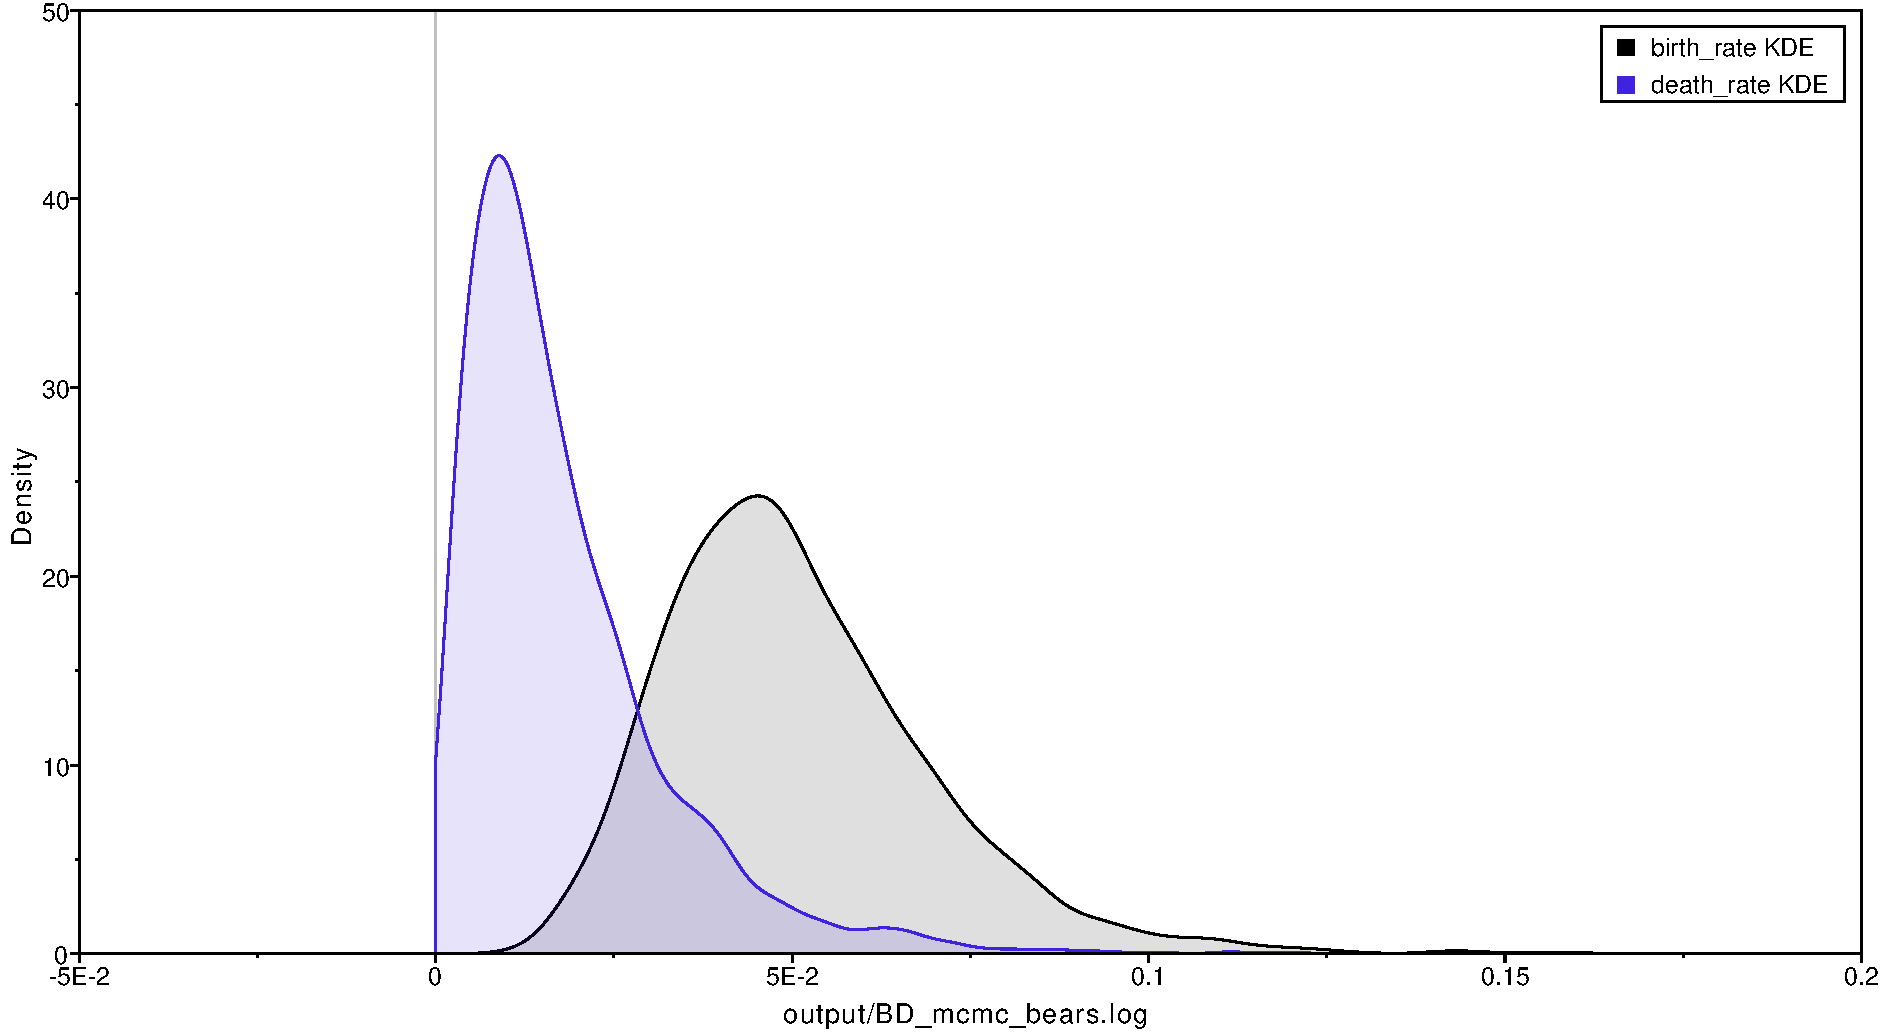
\includegraphics[width=4in]{figures/div_tracer.pdf}}
\caption{\small The marginal densities of \cl{birth\_rate} and \cl{death\_rate} estimated under the birth-death model in \RevBayes.}
\label{tracerMarg}
\end{figure}

\exs{Visualize the MCMC samples of the birth rate and death rate parameters in Tracer.}

\bigskip
\section*{Useful Links}

\begin{itemize}
\item RevBayes: \href{https://github.com/revbayes/revbayes}{https://github.com/revbayes/revbayes} \\ \vspace{-7mm}
\item TreePar: \href{http://cran.r-project.org/web/packages/TreePar/index.html}{http://cran.r-project.org/web/packages/TreePar/index.html} \\ \vspace{-7mm}
\item Tree Thinkers: \href{http://treethinkers.org/}{http://treethinkers.org} \\ \vspace{-7mm}
\end{itemize}

Questions about this tutorial can be directed to: \\\vspace{-10mm}
\begin{itemize}
\item Tracy Heath (email: \href{mailto:tracyh@berkeley.edu}{tracyh@berkeley.edu}) \\\vspace{-8mm}
\item Tanja Stadler (email: \href{mailto:tanja.stadler@bsse.ethz.ch}{tanja.stadler@bsse.ethz.ch}) \\\vspace{-8mm} 
\item Sebastian H\"{o}hna (email: \href{mailto:sebastian.hoehna@gmail.com}{sebastian.hoehna@gmail.com})
\end{itemize}



\newrefsection
\chapter{Gene tree - Species tree estimation}


\section{Overview: Gene tree-species tree models}

Ever since Zuckerkandl and Pauling \citep{Zuckerkandl1965a}, people have recognised that phylogenies reconstructed from homologous gene sequences could differ from species phylogenies.
As molecular sequences accumulated, the link between gene trees and species trees started to be modelled. 
The first models were based on parsimony, and aimed for instance at reconciling a gene tree with a species tree by minimizing the number of events of gene duplication and gene loss. 
In the past dozen years, probabilistic models have been proposed to reconstruct gene trees and species trees in a rigorous statistical framework.
Models and algorithms have quickly grown in complexity, to model biological processes with increasing realism, to accommodate several processes at the same time, or to handle genome-scale data sets.
In this overview we will not detail these models, and we invite the interested reader to take a look at recent reviews (e.g. \citep{Szollosi28072014}).

\subsection{Processes of discord}
There are several reasons why a gene tree may differ from a species tree. 
Of course, a gene tree may differ from the species tree just because a mistake was made during the analysis of the gene sequences, at any point in a pipeline going from the sequencing itself to the tree reconstruction.
Such a mistake would produce an incorrect gene tree.
Here we do not mean this kind of discord, but rather discord that has comes from a real biological process that builds true gene histories that differ from true species histories.
These processes include gene duplication, gene loss, gene transfer (used loosely here to also include reticulation, hybridization between species), and incomplete lineage sorting (Fig. \ref{fig1}). 
Incomplete lineage sorting will be discussed in more details in the following subsection.

\begin{figure}[h!]
\centering
\fbox{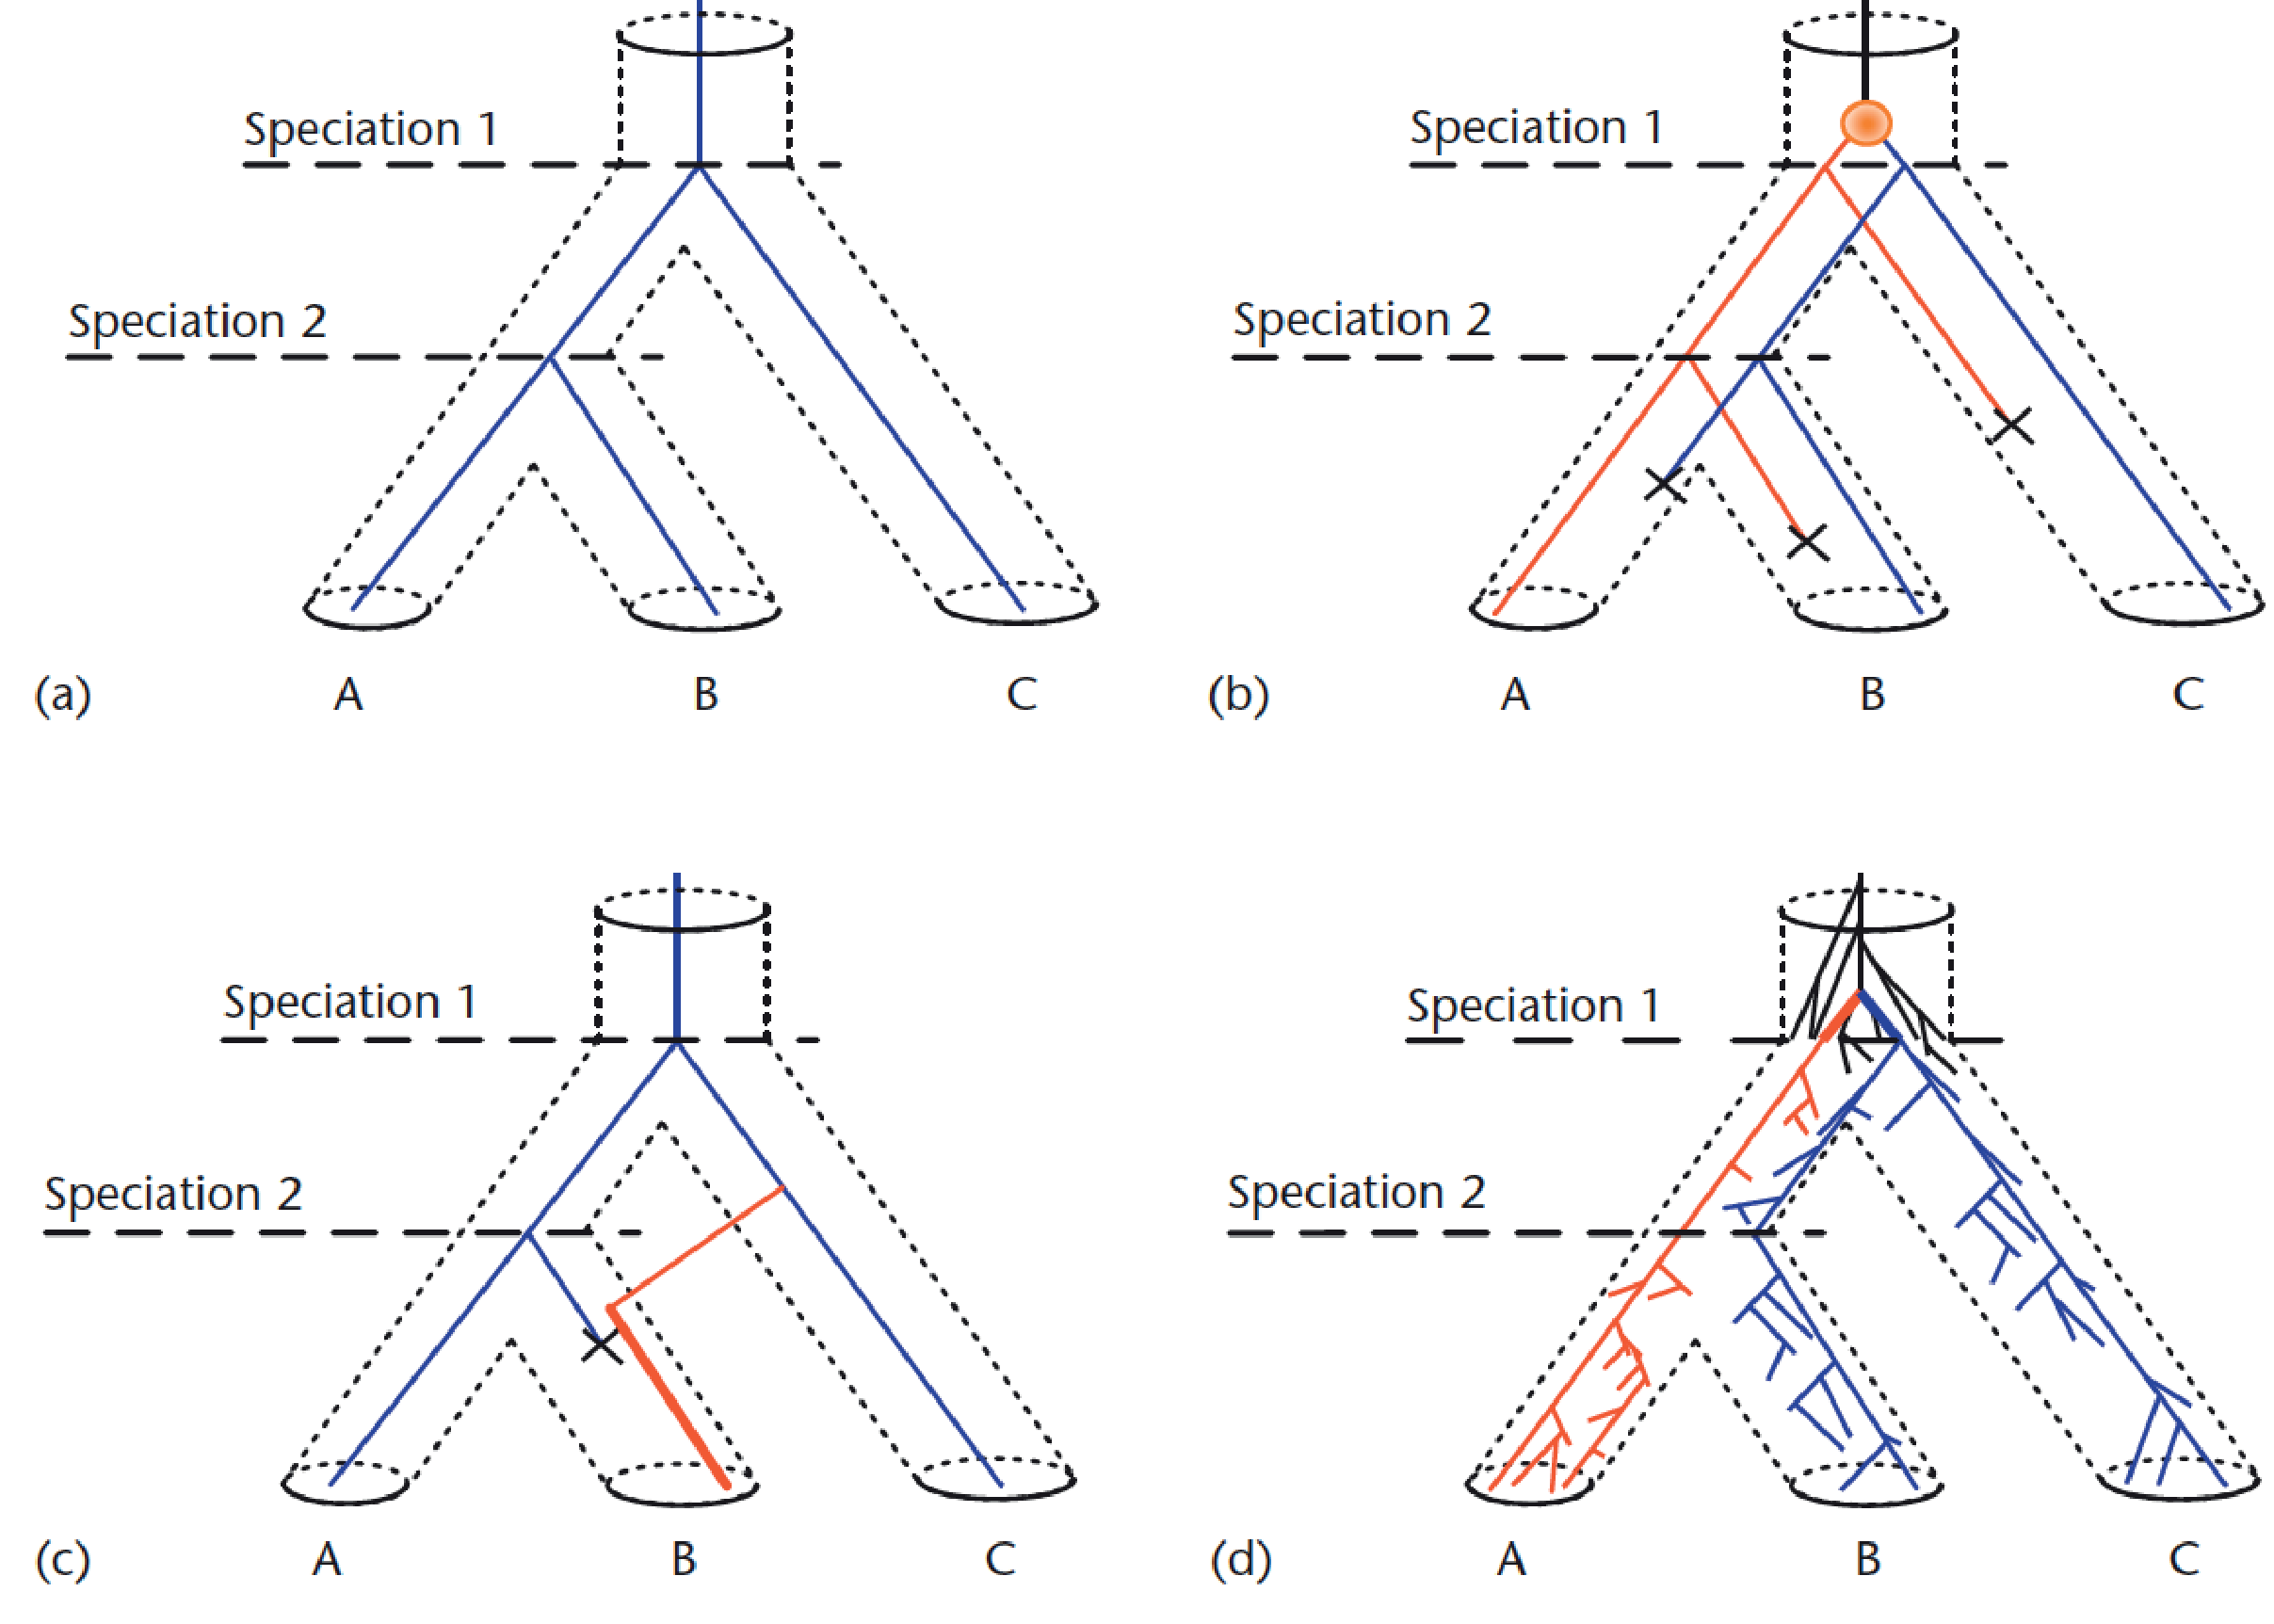
\includegraphics[width=5.8in,angle=0]{RB_GTST_Tutorial/figures/DupTransILS.pdf}}
\caption{\small The processes of discord. The species tree is represented as a tubular structure. Gene trees are blue and red lines running along the species trees. a) A gene tree that perfectly matches the species tree. b) The gene tree and the species tree differ because of gene duplications and losses. c)  The gene tree and the species tree differ because of gene transfer and gene loss. d)  The gene tree and the species tree differ because of incomplete lineage sorting.   [Replicated from Fig.~2 in \citet{Boussau2009}.]}
\label{fig1}
\end{figure}

Fig. \ref{fig1} suggests that for all processes the gene tree can be seen as the product of a branching process operating inside the species tree.
As a consequence, all processes are modelled as some type of birth-death process.
For duplication/loss models, birth correspond to gene duplication events, and death to gene loss events.
Transfers can be added to the model by introducing another type of birth, with a child lineage appearing in another branch of the species tree.
Incomplete lineage sorting is also modelled with a birth-death type of model, the coalescent.
All these models can be made heterogeneous, by allowing different sets of parameters for different branches of the species tree.
This is useful to model differences in rates of duplication, loss or transfer among species, or to model different effective population sizes in a species tree.
In RevBayes so far only models of incomplete lineage sorting have been implemented (models of duplication and loss and transfer will soon be added).
Thanks to RevBayes modular design, there is quite a lot of flexibility in specifying the model, for instance by allowing different parameters to different branches of the species tree, and the gene tree-species tree model could be combined to other types of models, for instance models of trait evolution.


\subsection{Gene tree discordance is a problem for species tree reconstruction}
There are several approaches to species tree reconstruction: concatenation and supertree approaches, which have been used for quite some time now, and more recently methods that rely on gene tree-species tree models.\begin{enumerate}
\item Concatenation simply consists in taking all gene alignments, concatenating them into one super alignment, and then analyzing it as if it were a single gene sequence.
Its main assumption is therefore that all sites of all genes have evolved according to the same species tree.
This assumption is not correct because all the processes of discord presented above conspire to make gene trees different from the species tree.
In practice, this matters: for instance, one can prove that in the presence of incomplete lineage sorting, in some particular area of the parameter space, concatenation will return an incorrect species tree.
Another example might be found in prokaryotic phylogenetics, where the quest for a tree of life has been very frustrating, to the point that many doubt that one could find a meaningful species tree representing vertical descent.
Recent models incorporating lateral gene transfer allow tackling this question in a more principled way.
\item Supertree approaches differ from concatenation notably by discarding sequence information once individual gene trees have been built.
They combine individual gene trees to obtain a species tree.
Most supertree methods are not based on an explicit model of the processes causing discordance between gene trees and species tree (although there are exceptions, notably modelling incomplete lineage sorting, see below).
Instead, they aim at finding a tree that would best describe the distribution of gene trees, according to some fairly arbitrary criterion.
In practice, these methods have been found to provide reasonable results in many cases, but in simulations are less accurate than concatenation.
\item Methods that rely on gene tree-species tree models appear very promising as they explicitly model the processes of discord, and can be combined with a model of sequence evolution, models of the co-evolution between gene trees, models of trait evolution... 
\end{enumerate}


\subsection{Modelling incomplete lineage sorting: the multispecies coalescent}
Incomplete lineage sorting is a population-level process.
In a species, at a given time, there are several alleles for a given locus in the genome.
These alleles have their own history, they diverged from each other at various times in the past.
This history can differ from the species history, because several alleles can persist through a speciation event, and because, short of selective effects, the sorting of alleles during a speciation event is random and can result in a tree that differs from the species tree (Fig. \ref{fig1}d).
In all cases, incongruence between the gene tree and the species tree occurs when alleles persist over the course of several speciation events.
When reconstructing a gene tree, one therefore gets the history of the alleles that have been sampled (at best), not necessarily the history of the species. 

In 2003, Rannala and Yang proposed a powerful way to model the sorting of alleles along a phylogeny of several species \citep{Rannala2003a}, the multispecies coalescent (Fig. \ref{fig2}).
This model is at the origin of most model-based approaches to reconstruct gene and species trees \citep{Edwards2007,Heled2010}.
The multispecies coalescent appropriately models the evolution of a population of alleles along a species tree.
Along the species tree, it allows different branch lengths, in units of time, and also allows different effective population sizes.
Computing the probability of a gene tree given a species tree and other parameters is quite easy.
Bascially it works by cutting the gene tree into independent species-specific subtrees, computing probabilities for each of those subtrees, and combining them all at the end to get the probability of the gene tree according to the multispecies coalescent, given the current parameter values.
Cutting the gene tree into species-specific subtrees is quite easy, because we can use the dates of speciation events to know what's before and after speciation events. 
The resulting subtrees are represented with the grey boxes in Fig. \ref{fig2}.
In this figure, each subtree corresponds to one particular population, either extant or ancestral.
Inside each subtree, given its length, the effective population size, and dates of coalescence (alleles splitting), the coalescent model provides simple formulas for computing the probability of the gene subtree given other parameters.
These subtree probabilities are then multiplied to get the gene tree probability given current parameter values.
 
Two parameters associated to branches of the species tree have a direct impact on the expected amount of gene tree-species tree incongruence:
\begin{itemize}
\item \textbf{Time between speciations.} The more a branch length increases, the more the pool of alleles is expected to change.
Alleles are therefore less likely to persist for several speciation events if the branches between these speciation events are long.
\item \textbf{Effective population size between speciations.} In populations with small effective population sizes, chance events can cause large shifts in allele frequencies, and possibly disappearance of alleles, irrespective of the fitness of this allele. 
In large populations, because an allele is likely carried by a large number of individuals, its disappearance is less likely, the population of alleles is more stable.
Alleles are therefore less likely to persist for several speciation events if the branches between these speciation events are characterised by small effective population sizes.
\end{itemize}
Overall, larger amounts of gene tree-species tree incongruence are expected in phylogenies characterised by short branches with large population sizes. 
A corollary of that is that larger amounts of gene tree-gene tree incongruence are expected as well. 
To measure the susceptibility of species phylogenies to generate incomplete lineage sorting, the concept of \emph{coalescent time units} has been introduced.
Coalescent time units are obtained when branch length $\lambda$ is divided by effective population size $N_e$.
As a consequence, in a species tree whose branches are expressed in coalescent time units, a branch length of $1~coalescent~time~unit $ means a branch length of $N_e~generations$. 
Once branch lengths on the species tree are measured in coalescent time units, it becomes easy to spot species trees that generate a lot of incongruence: those are short trees.

\begin{figure}[h!]
\centering
\fbox{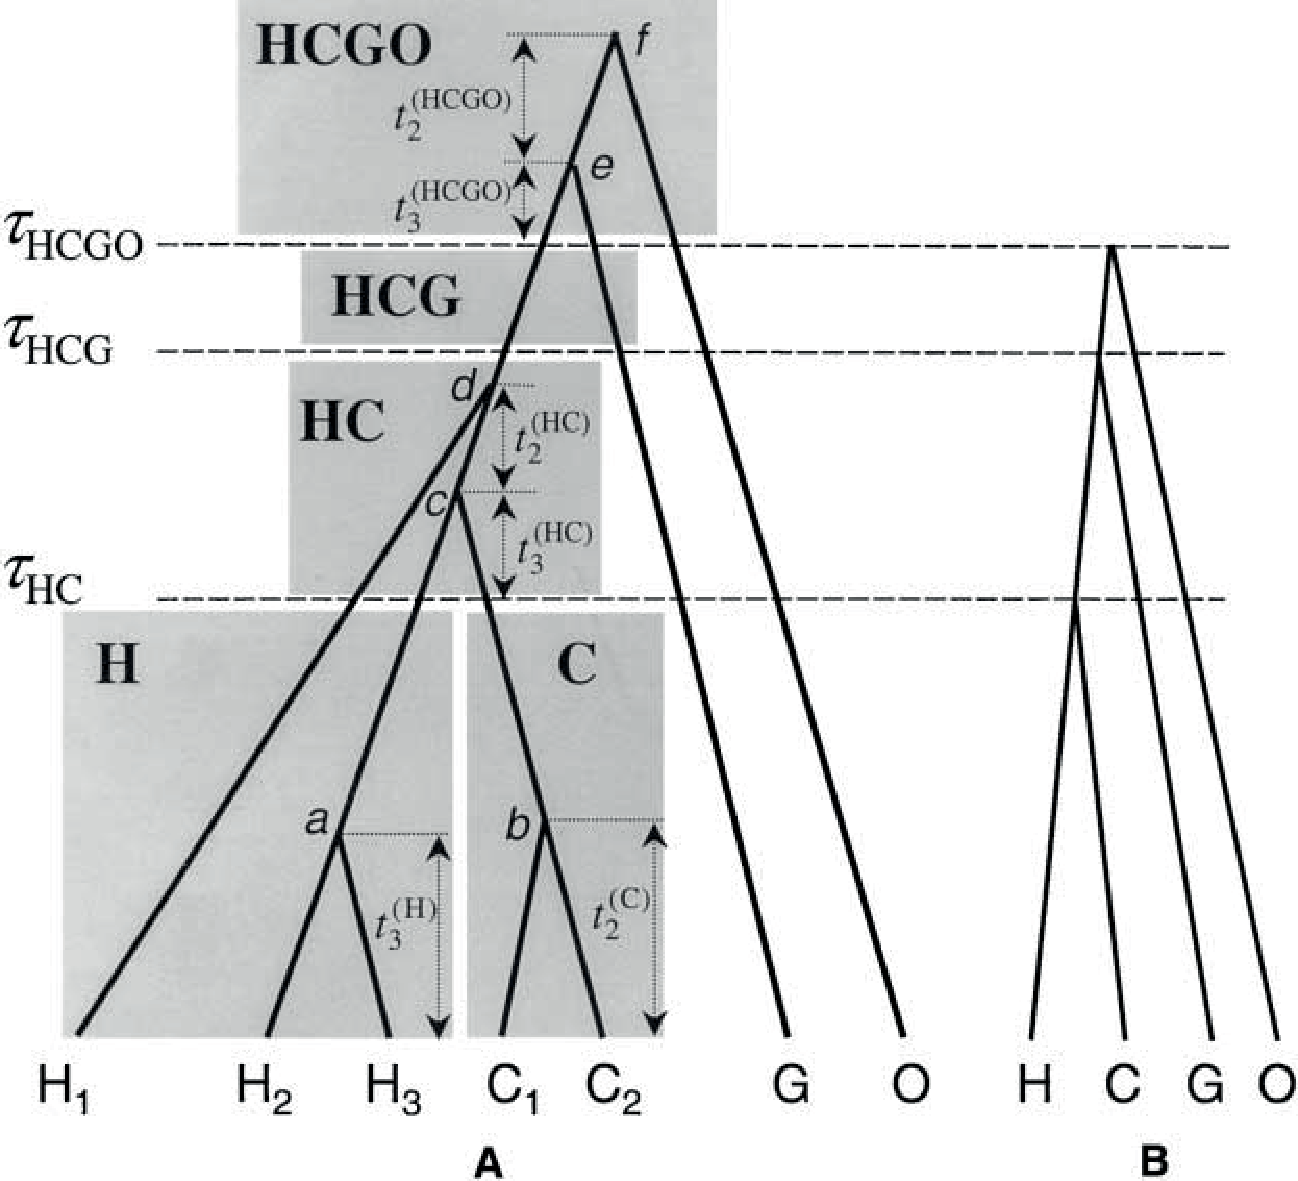
\includegraphics[width=5.8in,angle=0]{RB_GTST_Tutorial/figures/RannalaYang.pdf}}
\caption{\small The multispecies coalescent. A) A gene tree, including 3 human alleles, 2 Chimp alleles, one Gorilla allele, and one Orang-outan allele. $\tau$ parameters are speciation times, $t$ parameters are divergence time in the gene tree, the grey squares represent the ancestral populations, with their respeciive sizes.  B) The corresponding species tree. In this model, the speciation times define minimal boundaries for allele divergence times. [Replicated from Fig.~1 in \citet{Rannala2003a}.]}
\label{fig2}
\end{figure}

\vspace{20mm}

{\begin{framed}
\begin{center}
The exercises assume you have a working installation of RevBayes.
The first exercise aims at understanding the impact of the parameters of the multispecies coalescent.
The other exercises will introduce methods to reconstruct species trees and gene trees using the multispecies coalescent or closely-related models.
Scripts are all placed in {\footnotesize \emph{$tutorials/RB\_GeneTreeSpeciesTree\_Tutorial/RB\_GeneTreeSpeciesTree\_tutorial\_files/RevBayes\_scripts/$}}, in five folders. 
\emph{It is highly recommended to start RevBayes from each of these folders when doing the exercises.}
\end{center}
\end{framed}}
\vspace{5mm}

{\begin{framed}

\begin{center}
\emph{First RevBayes exercise: simulating gene trees under the multispecies coalescent}
\end{center}
\begin{enumerate}
\item Open RevBayes
\item Let's simulate a species tree with 10 taxa, 10 gene trees, 5 alleles per species (feel free to change these values).
{\tt \begin{snugshade*}
\begin{lstlisting}
n_species <- 10
n_genes <- 10
n_alleles <- 5

# Species names
for (i in 1:n_species) {
	s_names[i] <- "Species_"+i
}
\end{lstlisting}
\end{snugshade*}}
\item We simulate a species tree topology according to a birth-death process with arbitrary parameter values (similar to \citet{Leache2011}):
{\tt \begin{snugshade*}
\begin{lstlisting}
speciation ~ dnExp(10.0)
extinction ~ dnExp(10.0)
tree_height ~ dnUniform(0,1.0)
speciation.setValue(2)
extinction.setValue(0.3)
tree_height.setValue(0.8)
speciesTree ~ dnBDP(lambda=speciation, mu=extinction, origin=tree_height, nTaxa=n_species, names=s_names)
\end{lstlisting}
\end{snugshade*}}
\item Then we can use the multispecies coalescent model to generate gene trees. These can be examined using Figtree or NJplot or any other tree viewer, but we can also directly compute symmetric differences between these from RevBayes. First, we simulate a set of gene trees, using a single effective population size for all branches, and after having constructed a map between species names and gene names:
{\tt \begin{snugshade*}
\begin{lstlisting}
# Build the mapping between sequence names and species names.
for (i in 1:n_species) {
	for (j in 1:n_alleles) {
		taxa[(i-1)*n_alleles+j] <- taxon(taxonName=s_names[i]+"_"+j, speciesName=s_names[i])
	}
}
# Set the effective population size
Ne ~ dnGamma(shape=0.1,rate=0.1)
Ne.setValue(0.004)
# Simulate gene trees
for (i in 1:n_genes) {
   # The gene tree from the multispecies coalescent process
   # Note that if Ne had been a vector of effective population sizes instead of a single value, 
   # allowing 1 parameter per branch of the species tree, the same line would work.
   geneTrees[i] ~ dnCoalMultiSpeciesConst(speciesTree=speciesTree, Ne=Ne, taxa=taxa)
}
\end{lstlisting}
\end{snugshade*}}

We write the data to file,  in the "dataFolder" directory.
{\tt \begin{snugshade*}
\begin{lstlisting}

# We need to save the species tree and the gene trees
write(speciesTree, filename=dataFolder+"speciesTree")

# Saving the gene trees
for (i in 1:(n_genes)) {
	write(geneTrees[i], filename=dataFolder+"geneTree_"+i+".tree")
}

\end{lstlisting}
\end{snugshade*}}


\item We can compute symmetric differences between all these gene trees. The symmetric difference between two trees is the total number of partitions found in one tree but not in the other one. In our case, the maximal difference is as follows:
{\tt \begin{snugshade*}
\begin{lstlisting}
maxDiff <- 2 * (n_species*n_alleles - 2)
\end{lstlisting}
\end{snugshade*}}
\item That will give us a reference for comparing with the values we get on our gene trees. We can build a function for computing all pairwise symmetric differences between our gene trees, and getting the mean. Caveat: in the current state of the Rev language, we have to use variable names that have never been used before in the workspace (hence the use of "k" and "l" for loop indices instead of "i" and "j" that have been used before. Alternatively we could have done a "clear(i)" and a "clear(j)" if we really wanted to use these variable names). 

{\tt \begin{snugshade*}
\begin{lstlisting}
function RealPos symDiffVector ( TimeTree[] vec ) {
	ndiff <- 1
	for (k in 1:(vec.size()-1)) {
		for (l in (k+1):vec.size()) {
			diff[ndiff]<-symDiff (vec[k], vec[l])
			ndiff <- ndiff+1
		}
	}
	return (mean(diff))
}


#We can then use this function on our gene trees:
symDiffVector(geneTrees)
\end{lstlisting}
\end{snugshade*}}
\item Now to get a sense of how population size and branch lengths alter the gene tree distribution, we can relaunch the multispecies coalescent simulation (step 4) and look at the resulting gene trees after having rescaled the species tree or changed the effective population size. To do these little changes: 
 {\tt \begin{snugshade*}
\begin{lstlisting}
# Changing Ne: 
Ne.setValue(0.08)
#Rescaling the species tree:
speciesTree.rescale(0.1)
\end{lstlisting}
\end{snugshade*}}
\end{enumerate}
\emph{Using the functions above, it is possible to look at the species tree in coalescent time units (which is very convenient). How would you do that?}

\emph{Do these observations seem coherent with the multispecies coalescent presentation above?}
\end{framed}}



\bigskip
\section{Alternatives to the multispecies coalescent model}
\subsection{Strengths and weaknesses of the multispecies coalescent}

The multispecies coalescent model is an elegant model. 
As we have seen above, we can easily simulate data under this model.
Inference using this model, combined with a model of sequence evolution, is also possible, and when it works, is very informative.
Not only can we get a dated species tree and dated gene trees from the multispecies coalescent, we can also get extant and ancestral effective population sizes \citep{Edwards2007,Heled2010}.
However inferring many parameters is difficult, and convergence can be difficult to reach with such models.
In particular, the strong interdependence that exists between the gene trees and the species tree makes it easy for algorithms to fall into local maxima.
As a consequence, there are ongoing efforts to develop methods for which inference would be easier, albeit at the cost of approximations and simplifications.

\subsection{Alternatives to the multispecies coalescent}
An easy way to simplify the problem is to consider that parts of it are already solved.
For instance, several approaches assume that rooted gene trees are available.
The problem then becomes markedly easier, but inference is then highly dependent on the quality of the input gene trees. 
Often, such methods also make other simplifying assumptions, and e.g. do not try to estimate separately time and effective population sizes, but instead directly work with coalescent time units.
These methods usually are much faster than the multispecies coalescent, should be more robust against local maxima, but are less ambitious about the amount of information they can get from the data, and are can be sensitive to the quality of the input gene trees.

Another approach is to use methods that mathematically bypass estimating gene trees altogether.
To our knowledge, there are three such approaches: SNAPP \citep{Bryant2012}, POMO \citep{DeMaio2013}, and SVDQuartets \citep{Chifman2014}.
They differ in the way the algorithms work, but they are all based on the same idea, which is integrating out gene trees.
To achieve that they extend the model of sequence evolution, which usually models substitution events, to also model population-level processes.
In RevBayes, so far only the POMO model has been implemented and will be discussed in the following part.

\subsection{The POMO model}
POMO models allele frequency changes along with mutations with a single transition matrix.
It extends the usual $4\times4$ DNA substitution matrix to incorporate polymorphic states.
In doing so, it makes a first important approximation: it only considers biallelic states.
For instance, it considers sites at which either an A or a C is found in a population, but it won't consider sites at which 3 different states, e.g. A, C, T, are observed in a population.
Then it makes a second approximation, which introduces a single virtual population size in lieu of the branchwise effective population sizes.
This virtual population size is not inferred, but is fixed to some low number.
In practice, \citet{DeMaio2013} consider that a virtual population size of 10 individuals should produce good results.
This virtual population size directly constrains the types of polymorphic states that can be considered.
With 10 individuals for instance, only frequencies such as $(100\%A)$, $(10\%A, 90\%C)$, $(20\%A, 80\%C)$, $(30\%A, 70\%C)$, ..., $(90\%A, 10\%C)$, $(100\%C)$ can be considered.
The POMO matrix models transitions among all these states, polymorphic ones as well as monomorphic ones, and has a size that depends on the virtual population size.
For instance, with a virtual population size of 10 individuals, the POMO square matrix contains $58$ rows: 4 monomorphic states, plus 6 types of biallelic states ($AC, AG, AT, CG, CT, GT$) times 9 frequencies.
Additional assumptions of the POMO model include total independence among sites (no linkage among sites), and absence of mutations in biallelic states: transitions among biallelic states or from biallelic states to monoallelic states only occur through population-level changes in allele frequencies, not through mutation of one allele into another.
Mutations only occur to transit from a monoallelic state to a biallelic state.

The POMO model therefore makes several approximations to avoid estimating gene trees.
Fewer parameters need to be estimated, as neither gene trees nor population sizes are estimated, but other parameters can be introduced into the model.
For instance \citet{DeMaio2013} estimate 4 base fitness parameters, which they use to model GC-biased gene conversion, which tends to increase the GC content of recombining sequences.
In the RevBayes implementation of POMO, base fitnesses can be estimated as well.

\bigskip
\section{Inference using the multispecies coalescent, the POMO model, and basic concatenation}
In this section we will perform inference using the multispecies coalescent, the POMO model, and concatenation.
Depending on your machine and on the size of the data, successful inference may take some time.
If this tutorial is done in a classroom environment, it may be wise to convene with friends that one tries the multispecies coalescent model while another one tries the POMO model, and the third one tries the concatenation approach, and that results will be shared.
In case you want to compare the results between machines or between RevBayes sessions, you have to make sure that you are using the same random seed in all sessions. This is easily done by setting the seed using 
 {\tt \begin{snugshade*}
\begin{lstlisting}
seed(x, y)
\end{lstlisting}
\end{snugshade*}}
where $x$ and $y$ are two integer numbers of your choice.

First we will simulate data, and then we will perform inference using the three different approaches.

%%%%%%%%%%%%%%%%%%%%%%%%%%%%%%%%%%%%%%%%%%%
%%%%%%%%%%%%%%%%%%%%%%%%%%%%%%%%%%%%%%%%%%%
%%%%%%%%%%%%%%%%%%%%%%%%%%%%%%%%%%%%%%%%%%%
\subsection{Simulating data}
We are going to do inference on simulated data, as produced during the previous section.
However in addition to the species tree and the gene trees, we will be producing sequence data.
Below is the RevBayes code necessary to simulate all the data.
As before, parameters of the simulation can be changed as seems fit, but here we chose parameters that resemble \citet{Leache2011}.

{\begin{framed}
\begin{center}
\emph{WARNING: The following script may be less up to date than the simulation scripts named "UnderstandingMultiSpeciesCoalescent/MultiSpeciesCoalescentSimulatingTreesAndAlignments.Rev".}
\end{center}
\end{framed}}
\vspace{5mm}


{\begin{framed}
First we can set the folder in which we will save the output of our work.
 {\tt \begin{snugshade*}
\begin{lstlisting}
dataFolder<-"/PATH/TO/A/FOLDER/WHERE/TO/SAVE/THE/OUTPUT"
setwd(dataFolder)
\end{lstlisting}
\end{snugshade*}}

Let's simulate a species tree with 6 taxa, 10 gene trees, 5 alleles per species, and along each gene tree one gene alignment 200 bases long.
It's a small data set, designed for manageable inference during a tutorial, but patient users may want to simulate a larger data set.

 {\tt \begin{snugshade*}
\begin{lstlisting}
n_species <- 10
n_genes <- 10
n_alleles <- 5
n_sites <- 100
n_branches <- 2 * n_species - 3 # number of branches in a rooted tree
\end{lstlisting}
\end{snugshade*}}

The species-tree birth-death model:

 {\tt \begin{snugshade*}
\begin{lstlisting}
# Species names
for (i in 1:n_species) {
	s_names[i] <- "Species_"+i
}
speciation ~ dnExp(10.0)
extinction ~ dnExp(10.0)
tree_height ~ dnUniform(0,1.0)
speciation.setValue(2)
extinction.setValue(0.3)
tree_height.setValue(0.008)
# Species tree from birth-death process
speciesTree ~ dnBDP(lambda=speciation, mu=extinction, origin=tree_height, nTaxa=n_species, names=s_names)
# Making a backup for future reference:
trueSpeciesTree <- speciesTree
\end{lstlisting}
\end{snugshade*}}

The gene-tree multispecies coalescent model
 {\tt \begin{snugshade*}
\begin{lstlisting}
# Build the mapping between sequence names and species names.
for (i in 1:n_species) {
	for (j in 1:n_alleles) {
		taxa[(i-1)*n_alleles+j] <- taxon(taxonName=s_names[i]+"_"+j, speciesName=s_names[i])
	}
}
# Set the effective population size
Ne ~ dnGamma(shape=0.5,rate=0.5)
Ne.setValue(0.004)
# Simulate gene trees
for (i in 1:n_genes) {
   # The gene tree from the multispecies coalescent process
   # Note that if Ne had been a vector of effective population sizes, 
   # allowing 1 parameter per branch of the species tree, the same line would work.
   geneTrees[i] ~ dnCoalMultiSpeciesConst(speciesTree=speciesTree, Ne=Ne, taxa=taxa)
}
# Making a backup for future reference:
trueGeneTrees <- geneTrees
trueNe <- Ne
\end{lstlisting}
\end{snugshade*}}

Substitution models will all be based on the GTR model. However, the parameters of the models change from one gene family to the next.
 {\tt \begin{snugshade*}
\begin{lstlisting}
for (i in 1:n_genes) {
  er_prior[i] <- v(1,1,1,1,1,1)
  er[i] ~ dnDirichlet(er_prior[i])
  sf_prior[i] <- v(1,1,1,1)
  sf[i] ~ dnDirichlet(sf_prior[i])
  Q[i] := fnGTR(er[i],sf[i]) 
}
# Making a backup for future reference:
for (i in 1:n_genes) {
	trueEr[i] <- er[i]
	trueSf[i] <- sf[i]
}
\end{lstlisting}
\end{snugshade*}}

Then we assume a strict clock Model, but of course we could assume a relaxed clock.
Each gene family can have its own rate of evolution, drawn from an exponential distribution.
 {\tt \begin{snugshade*}
\begin{lstlisting}
for (i in 1:n_genes) {
  familyRates[i] ~ dnExp(1.0)
}
# Making a backup for future reference:
for (i in 1:n_genes) {
  trueFamilyRates[i] <- familyRates[i] 
}
\end{lstlisting}
\end{snugshade*}}

We add a model of among-site rate variation, handled by a discretized Gamma distribution, one for each gene family:

 {\tt \begin{snugshade*}
\begin{lstlisting}
for (i in 1:n_genes) {
  shape_prior[i] <- 0.05 
  shape[i] ~ dnExponential( shape_prior[i] )
  norm_gamma_rates[i] := fnDiscretizeGamma( shape[i], shape[i], 4, false )
}
\end{lstlisting}
\end{snugshade*}}

Finally we link it all using the PhyloCTMC model, which simulates gene alignments:

 {\tt \begin{snugshade*}
\begin{lstlisting}
for (i in 1:n_genes) {
  alns[i] ~ dnPhyloCTMC(tree=geneTrees[i], Q=Q[i],  branchRates=familyRates[i], siteRates=norm_gamma_rates[i], nSites=n_sites, type="DNA")
}
\end{lstlisting}
\end{snugshade*}}
We can then save the simulated data to the folder chosen at the beginning of this script.
We need to save the species tree, the gene trees, and the gene alignments

 {\tt \begin{snugshade*}
\begin{lstlisting}
write(speciesTree, filename="speciesTree")
for (i in 1:n_genes) {
	write(geneTrees[i], filename="geneTree_"+i)
}
for (i in 1:n_genes) {
	writeFasta(alns[i], filename="alignment_"+i+".fasta")
}
\end{lstlisting}
\end{snugshade*}}
\end{framed}}

%%%%%%%%%%%%%%%%%%%%%%%%%%%%%%%%%%%%%%%%%%%
%%%%%%%%%%%%%%%%%%%%%%%%%%%%%%%%%%%%%%%%%%%
%%%%%%%%%%%%%%%%%%%%%%%%%%%%%%%%%%%%%%%%%%%
\subsection{Inference using the multispecies coalescent }
{\begin{framed}
\begin{center}
\emph{WARNING: The following script may be less up to date than the simulation script named "MultiSpeciesCoalescentWithSequences/MultiSpeciesCoalescentWithSequencesMCMC.Rev".}
In the following we perform inference from the alignments, but we could also do inference directly from the gene trees, as can be seen in the script "MultiSpeciesCoalescent/MultiSpeciesCoalescentMCMC.Rev".
\end{center}
\end{framed}}
\vspace{5mm}


Now that we have simulated data, we can run inference under the multispecies coalescent, using the sequences as input data.

{\begin{framed}
First we clamp the alignments:
{\tt \begin{snugshade*}
\begin{lstlisting}
for (i in 1:n_genes) {
	alns[i].clamp(alns[i])
}
\end{lstlisting}
\end{snugshade*}}

Then we change the starting values, because we want to start from random values, not the values used in the simulation.

{\tt \begin{snugshade*}
\begin{lstlisting}
# Redrawing the parameters of the birth-death process:
speciation.redraw()
extinction.redraw()
tree_height.redraw()
# Redrawing the species tree:
speciesTree.redraw()
# Redrawing the parameter Ne:
Ne.redraw()
# Redrawing the gene trees:
for (i in 1:n_genes) {
   geneTrees[i].redraw()
}
# Redrawing the parameters of the substitution models:
for (i in 1:n_genes) {
  er[i].redraw()
  sf[i].redraw()
}
# Idem for the family-wise rates of sequence evolution:
for (i in 1:n_genes) {
  familyRates[i].redraw()
}
# Idem for the family-wise across-site rate variation parameters:
for (i in 1:n_genes) {
  shape[i].redraw()
}
\end{lstlisting}
\end{snugshade*}}

We need to set up moves for the birth-death parameters, the species tree topology, the gene tree topologies, the parameter Ne, the parameters of the substitution models, the rates on the gene trees.

{\tt \begin{snugshade*}
\begin{lstlisting}
moveIndex <- 0
# moves for the birth-death parameters
moves[moveIndex++] <- mvScale(speciation,1,true,1.0) # In the revLanguage, table indices start at 1
moves[moveIndex++] <- mvScale(extinction,1,true,1.0)
moves[moveIndex++] <- mvSlide(tree_height,delta=1.0,true,2.0)
# moves on the tree topology and node ages
moves[moveIndex++] <- mvNNI(speciesTree, 1.0)
moves[moveIndex++] <- mvFNPR(speciesTree, 1.0)
moves[moveIndex++] <- mvSubtreeScale(speciesTree, 5.0)
moves[moveIndex++] <- mvTreeScale(speciesTree, delta=1.0, tune=true, weight=3.0)
moves[moveIndex++] <- mvNodeTimeSlideUniform(speciesTree, 10.0)
moves[moveIndex++] <- mvRootTimeSlide(speciesTree, 1.0, true, 3.0)
# moves on the gene tree topologies and node ages
for (i in 1:n_genes) {
   moves[moveIndex++] <- mvNNI(geneTrees[i], 1.0)
   moves[moveIndex++] <- mvFNPR(geneTrees[i], 1.0)
   moves[moveIndex++] <- mvSubtreeScale(geneTrees[i], 5.0)
   moves[moveIndex++] <- mvTreeScale(geneTrees[i], delta=1.0, tune=true, weight=3.0)
   moves[moveIndex++] <- mvNodeTimeSlideUniform(geneTrees[i], 10.0)
   moves[moveIndex++] <- mvRootTimeSlide(geneTrees[i], 1.0, true, 3.0)
}
# move on Ne, the effective population size
moves[moveIndex++] <- mvScale(Ne,1,true,1.0)
# moves on the parameters of the substitution models
for (i in 1:n_genes) {
  moves[moveIndex++] <- mvSimplexElementScale(er[i], alpha=10, tune=true, weight=3) 
  moves[moveIndex++] <- mvSimplexElementScale(sf[i], alpha=10, tune=true, weight=2) 
}
# moves on the family-wise rates
for (i in 1:n_genes) {
  moves[moveIndex++] <- mvScale(familyRates[i], lambda=0.8, tune=true, weight=3.0)
}
# moves on the across-sites rate variation parameters:
for (i in 1:n_genes) {
  moves[moveIndex++] <- mvScale(shape[i], lambda=0.8, tune=true, weight=3.0)
}
\end{lstlisting}
\end{snugshade*}}

Then we define a few monitors to keep track of how things go. 
First, basic monitors:
{\tt \begin{snugshade*}
\begin{lstlisting}
mntrIndex <- 0
# One monitor to backup the parameters, in case we want to stop and restart the analysis:
monitors[mntrIndex++] <- mnModel(filename="multispeciesCoalescent_clock.log",printgen=10, separator = "	")
# One monitor to print the species trees sampled in the course of the MCMC:
monitors[mntrIndex++] <- mnFile(filename="multispeciesCoalescent_clock_species.trees",printgen=10, separator = "	", speciesTree)
# One monitor for each gene family tree:
for (i in 1:n_genes) {
   monitors[mntrIndex++] <- mnFile(filename="multispeciesCoalescent_clock_gene_"+ i +".trees",printgen=10, separator = "	", geneTrees[i])
}
\end{lstlisting}
\end{snugshade*}}
We will also compare our reconstructed parameters (trees or other variables) to the true values that were used in the simulation.
First, examining the species tree and the gene trees.
{\tt \begin{snugshade*}
\begin{lstlisting}
distSpeciesTree := symDiff (trueSpeciesTree, speciesTree)
for (i in 1:n_genes) {
	distGeneTree[i] := symDiff (trueGeneTrees[i], geneTrees[i])
}
# We get one average value for all gene trees:
meanDistGeneTree := mean(distGeneTree)
\end{lstlisting}
\end{snugshade*}}

We can also look at the values of some other variables:
{\tt \begin{snugshade*}
\begin{lstlisting}
# For Ne:
distNe := Ne - trueNe
# For equilibrium values of the GTR matrices, we want one index of how far we are.
# To achieve this we need to write some functions:
clear(i)
distEqFreq := diffVectorsOfVectors(trueSf, sf)	
function RealPos diffVectors ( Real[] xvec, Real[] yvec ) { 
	DI <- 0.0
	for (i in 1:xvec.size()) {
		DI <- DI + (xvec[i] - yvec[i])*(xvec[i] - yvec[i])
	}
	return DI
}
function RealPos diffVectorsOfVectors ( Real[][] xvecvec, Real[][] yvecvec ) { 
	DA <- 0.0
	for (i in 1:xvecvec.size()) {
		DA <- DA + diffVectors(xvecvec[i], yvecvec[i])
	}
	return DA
}		
function RealPos diffVectorsOfVectors ( Simplex[] xvecvec, Simplex[] yvecvec ) { 
	DA <- 0.0
	for (i in 1:xvecvec.size()) {
		DA <- DA + diffVectors(xvecvec[i], yvecvec[i])
	}
	return xvecvec[2]
}
# Same thing for exchangeability parameters:
distExchange := diffVectorsOfVectors(trueEr, er)
monitors[mntrIndex++] <- mnScreen(printgen=10, distExchange)
# Same thing for the family-wise rates
distRates := diffVectors(trueFamilyRates, familyRates)
monitors[mntrIndex++] <- mnScreen(printgen=10, distRates)
# We can use one monitor that will output on the screen one parameter, Ne, distNe, distSpeciesTree, meanDistGeneTree, and distEqFreq:
monitors[mntrIndex++] <- mnScreen(printgen=10, Ne, distNe, distSpeciesTree, meanDistGeneTree, distEqFreq)
# We could do similar things for the few remaining parameters, but really I think that's enough.
\end{lstlisting}
\end{snugshade*}}

We then define our model and the mcmc object. We can use any node of our model as a handle, here we choose to use the species tree.
{\tt \begin{snugshade*}
\begin{lstlisting}
mymodel <- model(speciesTree)
# We create the MCMC object
mymcmc <- mcmc(mymodel, monitors, moves)
\end{lstlisting}
\end{snugshade*}}

We finally launch the analysis.
{\tt \begin{snugshade*}
\begin{lstlisting}
# If we want to specify the amount of burnin:
# mymcmc.burnin(generations=200,tuningInterval=100)
mymcmc.run(generations=400)

\end{lstlisting}
\end{snugshade*}}


After the analysis, we analyze the output. We analyze the tree trace as saved in one of the output files.
{\tt \begin{snugshade*}
\begin{lstlisting}
# Let us start by reading in the tree trace
 treetrace <- readTreeTrace("multispeciesCoalescent_clock_species.trees")
# and get the summary of the tree trace
 treetrace.summarize()

# We output the Maximum A Posteriori tree
 mapTree(treetrace,"primates_clock_MAP.tre")

\end{lstlisting}
\end{snugshade*}}

Of course, we could do the same analysis with each of the gene trees, possibly using a "for" loop in the rev language.

\end{framed}}

%%%%%%%%%%%%%%%%%%%%%%%%%%%%%%%%%%%%%%%%%%%
%%%%%%%%%%%%%%%%%%%%%%%%%%%%%%%%%%%%%%%%%%%
%%%%%%%%%%%%%%%%%%%%%%%%%%%%%%%%%%%%%%%%%%%
\subsection{Inference using the POMO model }

{\begin{framed}
\begin{center}
\emph{WARNING: The following script may be less up to date than the simulation script named "MultiSpeciesCoalescentAndPomo/MultiSpeciesCoalescentPomoMCMC.Rev".}
\end{center}
\end{framed}}
\vspace{5mm}


We run the POMO model on the same data set simulated under the multispecies coalescent.
 {\begin{framed}
 First, we need to prepare the data for analysis using POMO: concatenating the alignments, then transforming the state space from 4 bases to the POMO state space.
 We arbitrarily decide to use a virtual population size of size 10, as suggested in \citet{DeMaio2013}.
 {\tt \begin{snugshade*}
\begin{lstlisting}
# First, concatenating the alignments:
concatenate<-alns[1]
for (i in 2:n_genes) {
	concatenate <- concatenate + alns[i]
}

virtual_population_size <- 10

# Now, we need to convert the DNA alignment into an alignment in the correct POMO state space.

pomo_concatenate <- pomoStateConvert(concatenate, virtual_population_size, taxa)
concatenate_n_sites <- pomo_concatenate.nchar()[1]
\end{lstlisting}
\end{snugshade*}}
Now we have the data for doing inference using the POMO model.
To define a POMO model, one needs several components.
First, one needs to define a transition matrix for DNA mutations.
Here we are going to use a GTR matrix. 

 {\tt \begin{snugshade*}
\begin{lstlisting}


er_prior <- v(1,1,1,1,1,1)
er ~ dnDirichlet(er_prior)

sf_prior <- v(1,1,1,1)
sf ~ dnDirichlet(sf_prior)

Q := fnGTR(er,sf) 
\end{lstlisting}
\end{snugshade*}}

Second, one can have different fitnesses for A, C, G, T. 
Here, we are going to assume that all 4 bases have the same fitness.

 {\tt \begin{snugshade*}
\begin{lstlisting}
base_fitnesses <- v(1, 1, 1, 1)
\end{lstlisting}
\end{snugshade*}}
Now we have all the elements to build a POMO matrix to model the evolution of a population of alleles along a species tree.
 {\tt \begin{snugshade*}
\begin{lstlisting}
P := fnPomo(Q, base_fitnesses, virtual_population_size)
\end{lstlisting}
\end{snugshade*}}

We also need to define root frequencies for all the states.
To do that we need two variables:

 {\tt \begin{snugshade*}
\begin{lstlisting}
# First, the proportion of polymorphic sites at the root
root_polymorphism_proportion ~ dnBeta(alpha=1,beta=1)

# Second, one needs the root frequencies (we could use those of the GTR matrix but choose to have a non-stationary model):
root_base_frequencies ~ dnDirichlet(sf_prior)
\end{lstlisting}
\end{snugshade*}}

Now we have all the elements to construct root frequencies for all the states:
 {\tt \begin{snugshade*}
\begin{lstlisting}

root_frequencies := pomoRF (root_base_frequencies, root_polymorphism_proportion, Q, virtual_population_size)
#simplex_root_frequencies := simplex(root_frequencies[1], root_frequencies[2], root_frequencies[3], root_frequencies[4])

\end{lstlisting}
\end{snugshade*}}

Adding an across site rate variation model, the usual Gamma distribution discretized in 4 categories:
 {\tt \begin{snugshade*}
\begin{lstlisting}

shape_prior <- 0.05 
shape ~ dnExponential( shape_prior )
norm_gamma_rates := fnDiscretizeGamma( shape, shape, 4, false )

# We do not assume variation among branches in rates
branch_rates <- 1.0

# We do not assume a proportion of invariant
p_inv ~ dnBeta(alpha=1,beta=1)
p_inv.setValue(0.000001)
\end{lstlisting}
\end{snugshade*}}

Combining it all with the PhyloCTMC Model and clamp the model to the data:
 {\tt \begin{snugshade*}
\begin{lstlisting}

aln ~ dnPhyloCTMC(tree=speciesTree, Q=P, rootFreq=root_frequencies, branchRates=branch_rates, siteRates=norm_gamma_rates, pInv=p_inv, nSites=concatenate_n_sites, type="Standard")

aln.clamp(pomo_concatenate)
\end{lstlisting}
\end{snugshade*}}

Changing the starting values, we want to start from random values, not the values used in the simulation:

 {\tt \begin{snugshade*}
\begin{lstlisting}

# Redrawing the parameters of the birth-death process:
speciation.redraw()
extinction.redraw()
tree_height.redraw()

# Redrawing the species tree:
speciesTree.redraw()


\end{lstlisting}
\end{snugshade*}}


Then we need to set up moves for the birth-death parameters, the species tree topology, the gene tree topologies, the parameter Ne, the parameters of the substitution models, the rates on the gene trees.
 {\tt \begin{snugshade*}
\begin{lstlisting}

moveIndex <- 0

# moves for the birth-death parameters
moves[moveIndex++] <- mvScale(speciation,1,true,1.0) # In the revLanguage, table indices start at 1
moves[moveIndex++] <- mvScale(extinction,1,true,1.0)
moves[moveIndex++] <- mvSlide(tree_height,delta=1.0,true,2.0)


# moves on the tree topology and node ages
moves[moveIndex++] <- mvNNI(speciesTree, 1.0)
moves[moveIndex++] <- mvFNPR(speciesTree, 1.0)
moves[moveIndex++] <- mvSubtreeScale(speciesTree, 5.0)
moves[moveIndex++] <- mvTreeScale(speciesTree, delta=1.0, tune=true, weight=3.0)
moves[moveIndex++] <- mvNodeTimeSlideUniform(speciesTree, 10.0)
moves[moveIndex++] <- mvRootTimeSlide(speciesTree, 1.0, true, 3.0)

# moves on the parameters of the substitution model
moves[moveIndex++] <- mvSimplexElementScale(er, alpha=10, tune=true, weight=3) 
moves[moveIndex++] <- mvSimplexElementScale(sf, alpha=10, tune=true, weight=2) 

# moves on the 4 fitness values
# SH: These are not stochastic nodes, so moves cannot operate on them!
#moves[moveIndex++] <- mvScale(base_fitnesses[1],1,true,1.0)
#moves[moveIndex++] <- mvScale(base_fitnesses[2],1,true,1.0)
#moves[moveIndex++] <- mvScale(base_fitnesses[3],1,true,1.0)
#moves[moveIndex++] <- mvScale(base_fitnesses[4],1,true,1.0)

# moves on the parameters of the root frequencies
moves[moveIndex++] <- mvSimplexElementScale(root_base_frequencies, alpha=10, tune=true, weight=3) 
#moves[moveIndex++] <- mvScale(root_polymorphism_proportion, lambda=10, tune=true, weight=2) 
moves[moveIndex++] <- mvSlide(root_polymorphism_proportion, delta=10, tune=true, weight=2) 

# moves on the across-sites rate variation parameter:
moves[moveIndex++] <- mvScale(shape, lambda=0.8, tune=true, weight=3.0)
\end{lstlisting}
\end{snugshade*}}

Then we define a few monitors to keep track of how things go:
 {\tt \begin{snugshade*}
\begin{lstlisting}
mntrIndex <- 0

# One monitor to backup the parameters, in case we want to stop and restart the analysis:
monitors[mntrIndex++] <- mnModel(filename="pomo_clock.log",printgen=10, separator = "	")

# One monitor to print the species trees sampled in the course of the MCMC:
monitors[mntrIndex++] <- mnFile(filename="pomo_clock_species.trees",printgen=10, separator = "	", speciesTree)

# We also want to monitor how far we are from the true values, which we have because we rely on simulations.
# First, we can compute the distance between the reconstructed and the true species tree:
distSpeciesTree := symDiff (trueSpeciesTree, speciesTree)


# We can use one monitor that will output on the screen one parameter, Ne, distNe, distSpeciesTree, meanDistGeneTree, and distEqFreq:
monitors[mntrIndex++] <- mnScreen(printgen=10, distSpeciesTree)
\end{lstlisting}
\end{snugshade*}}
We define our model:
 {\tt \begin{snugshade*}
\begin{lstlisting}
# First we need to get rid of several variables that are not part of the Pomo model.
clear(alns)
clear(geneTrees)
clear(Ne)
clear(familyRates)
clear(trueEr)
clear(trueFamilyRates)
clear(trueGeneTrees)
clear(trueNe)
clear(trueSf)

# We can use any node of our model as a handle, here we choose to use the species tree.
 
mymodel <- model(speciesTree)
\end{lstlisting}
\end{snugshade*}}

We create and run the MCMC object

 {\tt \begin{snugshade*}
\begin{lstlisting}
mymcmc <- mcmc(mymodel, monitors, moves)
# mymcmc.burnin(generations=200,tuningInterval=100)
mymcmc.run(generations=40000)
\end{lstlisting}
\end{snugshade*}}
 \end{framed}}

\subsection{Inference using basic concatenation }

{\begin{framed}
\begin{center}
\emph{WARNING: The following script may be less up to date than the simulation scripts named "MultiSpeciesCoalescentAndConcatenation/MultiSpeciesCoalescentConcatenationMCMC.Rev".}
\end{center}
\end{framed}}
\vspace{5mm}
We can also concatenate all alignments and run a partitioned GTR model on it.


 {\begin{framed}
 {\tt \begin{snugshade*}
\begin{lstlisting}

# Birth-Death process priors.
speciation ~ dnExp(10.0)
extinction ~ dnExp(10.0)
tree_height ~ dnUniform(0.0,100.0)
speciation.setValue(2)
extinction.setValue(0.3)

# Species tree from birth-death process
#We assume 1000,000 generations
speciesTree ~ dnBDP(lambda=speciation, mu=extinction, rootAge=tree_height, nTaxa=n_species, names=s_names)
\end{lstlisting}
\end{snugshade*}}
Second, one needs to define a transition matrix for DNA mutations, and we use a GTR matrix for that.

 {\tt \begin{snugshade*}
\begin{lstlisting}
er_prior <- v(1,1,1,1,1,1)
er ~ dnDirichlet(er_prior)

sf_prior <- v(1,1,1,1)
sf ~ dnDirichlet(sf_prior)

Q := fnGTR(er,sf) 
\end{lstlisting}
\end{snugshade*}}

Adding an across site rate variation model, the usual Gamma distribution discretized in 4 categories.
 {\tt \begin{snugshade*}
\begin{lstlisting}
shape_prior <- 0.05 
shape ~ dnExponential( shape_prior )
norm_gamma_rates := fnDiscretizeGamma( shape, shape, 4, false )

# We do not assume variation among branches in rates
branch_rates <- 1.0

# We do not assume a proportion of invariant
p_inv ~ dnBeta(alpha=1,beta=1)
p_inv.setValue(0.000001)
\end{lstlisting}
\end{snugshade*}}

To link all the parts of the model together we use the phyloCTMC object and clamp it to the concatenate.

 {\tt \begin{snugshade*}
\begin{lstlisting}


aln ~ dnPhyloCTMC(tree=speciesTree, Q=Q, branchRates=branch_rates, siteRates=norm_gamma_rates, pInv=p_inv, type="DNA")

aln.clamp( concatenate )
\end{lstlisting}
\end{snugshade*}}

Then we define the moves.

 {\tt \begin{snugshade*}
\begin{lstlisting}

moveIndex <- 0

# moves for the birth-death parameters
moves[moveIndex++] <- mvScale(speciation,lambda=1,tune=true,weight=1.0) # In the revLanguage, table indices start at 1
moves[moveIndex++] <- mvScale(extinction,1,true,1.0)
moves[moveIndex++] <- mvSlide(tree_height,delta=1.0,true,2.0)

# moves on the tree topology and node ages
moves[moveIndex++] <- mvNNI(speciesTree, 2.0)
moves[moveIndex++] <- mvNarrow(speciesTree, 5.0)
moves[moveIndex++] <- mvFNPR(speciesTree, 2.0)
moves[moveIndex++] <- mvSubtreeScale(speciesTree, 5.0)
moves[moveIndex++] <- mvTreeScale(speciesTree, tree_height, delta=1.0, tune=true, weight=3.0)
moves[moveIndex++] <- mvNodeTimeSlideUniform(speciesTree, 10.0)

# moves on the parameters of the substitution model
moves[moveIndex++] <- mvSimplexElementScale(er, alpha=10, tune=true, weight=3) 
moves[moveIndex++] <- mvSimplexElementScale(sf, alpha=10, tune=true, weight=2) 

# moves on the across-sites rate variation parameter:
moves[moveIndex++] <- mvScale(shape, lambda=0.8, tune=true, weight=3.0)
\end{lstlisting}
\end{snugshade*}}

We define a few monitors to keep track of how things go.
 {\tt \begin{snugshade*}
\begin{lstlisting}

mntrIndex <- 0

# One monitor to backup the parameters, in case we want to stop and restart the analysis:
monitors[mntrIndex++] <- mnModel(filename=dataFolder+"concatenation_clock.log",printgen=10, separator = "	")

# One monitor to print the species trees sampled in the course of the MCMC:
monitors[mntrIndex++] <- mnFile(filename=dataFolder+"concatenation_clock_species.trees",printgen=10, separator = "	", speciesTree)

# We also want to monitor how far we are from the true values, which we have because we rely on simulations.
# First, we can compute the distance between the reconstructed and the true species tree:
distSpeciesTree := symDiff (trueSpeciesTree, speciesTree)


# We can use one monitor that will output on the screen one parameter, Ne, distNe, distSpeciesTree:
monitors[mntrIndex++] <- mnScreen(printgen=10, distSpeciesTree)
	
\end{lstlisting}
\end{snugshade*}}
We define the model and launch the MCMC.

 {\tt \begin{snugshade*}
\begin{lstlisting}
mymodel <- model(speciesTree)

# We create the MCMC object
mymcmc <- mcmc(mymodel, monitors, moves)

#mymcmc.burnin(generations=200,tuningInterval=100)
mymcmc.run(generations=4000)


\end{lstlisting}
\end{snugshade*}}

 \end{framed}}

\bigskip


\section{Batch Mode}

If you wish to run these exercises in batch mode, the files are provided for you. 

You can carry out these batch commands by providing the file name when you execute the \cl{rb} binary in your unix terminal (this will overwrite all of your existing run files).
\exs{\cl{\$ rb NameOfTheFile.Rev}}


\section{Things to think about}
How did the different methods perform? 
Did you expect to see these differences?
It has been shown that the concatenation approach could be inconsistent under some conditions of population size and of divergence times \citep{Degnan2006}. 
Do you find that concatenation performs worse that its competitors?
Which models seem to "mix" better?
In particular, does the full multispecies coalescent mix well?
Why can we expect this model in particular would have difficulties mixing?


\bigskip
\section{Useful Links}

\begin{itemize}
\item RevBayes: \href{https://github.com/revbayes/code}{https://github.com/revbayes/code} \\ \vspace{-7mm}
\item Tree Thinkers: \href{http://treethinkers.org/}{http://treethinkers.org} \\ \vspace{-7mm}
\item NJplot, a lightweight tree plotting program: \href{http://doua.prabi.fr/software/njplot}{http://doua.prabi.fr/software/njplot} \\ \vspace{-7mm}
\item Seaview, a program to handle alignments and trees: \href{http://doua.prabi.fr/software/seaview}{http://doua.prabi.fr/software/seaview} \\ \vspace{-7mm}

\end{itemize}

Questions about this tutorial can be directed to: \\\vspace{-10mm}
\begin{itemize}
\item Bastien Boussau (email: \href{mailto:boussau@gmail.com}{boussau@gmail.com}) \\\vspace{-8mm}
\item Sebastian H\"{o}hna (email: \href{mailto:sebastian.hoehna@gmail.com}{sebastian.hoehna@gmail.com})
\end{itemize}

\href{http://creativecommons.org/licenses/by/4.0/}{
\includegraphics[scale=0.8]{shared_figures/ccby.eps}}This tutorial was written by \href{http://phylo.bio.ku.edu/content/tracy-heath}{Bastien Boussau}; licensed under a \href{http://creativecommons.org/licenses/by/4.0/}{Creative Commons Attribution 4.0 International License}. 

Version dated: \today


\bibliographystyle{mbe}
\bibliography{bib_tex/master_refs}

%\nocite{sukumaran10,rannala96,robert02,rodrigue08,ronquist09,Rubinstein1981,simon01,Smith1993,Suchard2005,verdinelli95,wong08,Yang2007,Yang2005,yang97b}
%\newpage

%%%%%%%%%%%%%%%%%%%%%%%%%%%%%%%%%%%%
%  REFERENCES  
%%%%%%%%%%%%%%%%%%%%%%%%%%%%%%%%%%%%

%{\renewcommand{\bibsection}{\section*{Relevant References}}


%\bibliography{bib_tex/biblio.bib}





\newrefsection
\chapter{Biogeography}

\section{Introduction}

This lab describes how to perform Bayesian inference of historical biogeography using RevBayes. The analysis jointly infers the posterior range evolution parameters and ancestral ranges using the data augmentation approach described in \citet{landis13}.
To examine the posterior, we'll use Python scripts, Tracer by Andrew Rambaut, to summarize MCMC output files, and Phylowood, a Javascript web service that animates and filters phylogenetic biogeography reconstructions \citep{landis14}.


\subsection*{\textbf{Outline}}
\begin{tabular}{ll}
{\bf I. Introduction} & \\
& a) Workspace setup \\
& b) Range evolution models and data augmentation \\
{\bf II. DEC in RevBayes} & \\
& a) Tree, range, and geographic input \\
& b) DEC as a graphical model \\
& c) Monitors, moves, and MCMC \\
& d) Model selection with Bayes factors \\
{\bf III. Output and Analysis} & \\
& a) MCMC output in Tracer \\
& b) Ancestral range output \\
& c) Animate ancestral ranges \\
\end{tabular}

%\noindent \\ \impmark These little arrows indicate lines containing key information to progress through the lab. The rest of the text gives context for why we're taking these steps or what to make of results.

\subsection{Handy links for this lab}

\begin{tabular}{ll}
RevBayes & \url{https://github.com/revbayes/revbayes} \\
Lab zip file & \href{https://github.com/revbayes/revbayes/raw/development/tutorials/RB\_Biogeography\_tutorial/RB\_biogeo\_files.zip}{{\tt https://github.com/revbayes/revbayes/.../RB\_biogeo\_files.zip}} \\
Phylowood software & \url{http://mlandis.github.io/phylowood} \\
Phylowood manual & \url{https://github.com/mlandis/phylowood/wiki} \\
Tracer & \url{http://tree.bio.ed.ac.uk/software/tracer}
%DendroPy manual & \url{http://pythonhosted.org/DendroPy/} \\
%matplotlib manual & \url{http://matplotlib.org/} \\
%NumPy manual & \url{http://www.numpy.org/}

\end{tabular}

\subsection{Setting up your workspace}

The practical part of the lab will analyze a small dataset of 19 taxa distributed over 4 biogeographic areas.
Parts of the lab will require entering terminal commands, which will assume you are using the Unix shell \texttt{bash}.
Just ask for help if the commands don't seem to work.

%\noindent \\ \impmark Portions of this lab require Python is installed. No packages are needed.

%\noindent \\ \impmark This tutorial will assume you have successfully installed RevBayes and can be called from your current working directory.

%\noindent \\ \impmark Download and unzip the lab zip file, {\tt RB\_biogeo\_files.zip}.


%%%%%%%%%%%%%%%%
%%%%%%%%%%%%%%%%
\section{Model and method}

This section contains a brief description of the data, model, parameters, and method used in BayArea.

First, we define the range for taxon $i$ as the bit vector $X_i$, where $X_{i,j} = 1$ if the taxon is present in area $j$ and $X_{i,j} = 0$ if the taxon is absent.
Each taxon range is a bit vector of length $N$ areas.
For example, if taxon $B$ is present only in areas 2 and 3 out of $N=3$ areas, its range is represented as $X_B = (0,1,1)$, which is translated to the bit string $X_B=011$ for short.
The data matrix, $\textbf{X}$, is analogous to a multiple sequence alignment where each element in the data matrix reports a discrete value for a homologous character shared by all taxa at column $j$.

Next, we need a model of range evolution.
Since we have discrete characters we'll use the continuous-time Markov chain, which allows us to compute transition probability of a character changing from $i$ to $j$ in time $t$ through matrix exponentiation
\[
\mathbf{P}_{i,j}(t) = \left[ \exp \left\lbrace \mathbf{Q}t \right\rbrace \right]_{i,j},
\]
where $\textbf{Q}$ is the instantaneous rate matrix defining the rates of change between all pairs of characters, and $\textbf{P}$ is the transition probability rate matrix.
This technique of matrix exponentiation is powerful because it integrates over all possible scenarios of character transitions that could occur during $t$ so long as the chain begins in state $i$ and ends in state $j$.

We can then encode range evolution events into the allowed character transitions of $\textbf{Q}$ and parameterize the events so that we may infer their relative importance to generating our observed ranges.
We'll take a simple model of range expansion (e.g. $011 \rightarrow 111$) and range contraction (e.g. $011 \rightarrow 001$).
(Range expansion may also be referred to as dispersal or area gain and range contraction as extirpation or area loss.)
The rates in the transition matrix for three areas might appear as

\[
\textbf{Q} = 
	\begin{array}{r|cccccccc}
		& 000 & 001 & 010 & 011 & 100 & 101 & 110 & 111 \\
		\hline
		000 & - & 0 & 0 & 0 & 0 & 0 & 0 & 0 \\
		001 & \lambda_0 & - & 0 & \lambda_1 & 0 & \lambda_1 & 0 & 0 \\
		010 & \lambda_0 & 0 & - & \lambda_1 & 0 & 0 & \lambda_1 & 0 \\
		011 & 0 & \lambda_0 & \lambda_0 & - & 0 & 0 & 0 & \lambda_1 \\
		100 & \lambda_0 & 0 & 0 & 0 & - & \lambda_1 & \lambda_1 & 0 \\
		101 & 0 & \lambda_0 & 0 & 0 & \lambda_0 & - & 0 & \lambda_1 \\
		110 & 0 & 0 & \lambda_0 & 0 & \lambda_0 & 0 & - & \lambda_1 \\
		111 & 0 & 0 & 0 & \lambda_0 & 0 & \lambda_0 & \lambda_0 & - \\								
	\end{array},
\]
where $\lambda_1$ and $\lambda_0$ are the rates of area gain and loss, respectively.
This matrix can be represented compactly as the rate function
\[
q^{(a)}_{\textbf{y},\textbf{z}} =
\begin{cases}
\lambda_0 & \text{if $z_a=0$}  \\
\lambda_1 & \text{if $z_a=1$} \\
0 & \text{\textbf{y} and \textbf{z} differ in more than one area}
\end{cases}.
\]

where $\textbf{y}$ and $\textbf{z}$ are the ``from'' and ``to'' ranges and $a$ is the area that changes.
For example, $q^{(1)}_{011,111}$ is the rate of range expansion for $011 \rightarrow 111$ to gain area $1$.
Note the rate of more than one event occurring simultaneously is zero, so a range must expand twice by one area in order to expand by two areas.
This model is analogous to the Jukes-Cantor model for three independent characters with binary states, except the all-zero ``null range'' is forbidden.

Lastly, we may reasonably expect that a range expansion event into an area depends on which nearby areas are currently inhabited, which imposes non-independence between characters.
The transition rate might then appear as
\[
q^{(a)}_{\textbf{y},\textbf{z}} =
\begin{cases}
\lambda_0 & \text{if $z_a=0$}  \\
\lambda_1 \eta(\textbf{y}, \textbf{z}, a, \beta) & \text{if $z_a=1$} \\
0 & \mathbf{y} = 00...0 \\
0 & \text{\textbf{y} and \textbf{z} differ in more than one area}
\end{cases}.
\]

For this tutorial, you can take $\eta(\cdot)$ to adjust the rate of range expansion into area $a$ by considering how close it is to the current range, $\textbf{y}$ relative to the closeness of all other areas unoccupied by the taxon.
The $\beta$ parameter rescales the importance of geographic distance between two areas by a power law.
Importantly, $\eta(\cdot) = 1$ when $\beta=0$, meaning geographic distance between areas is irrelevant.
Moreover, when $\beta > 0$, $\eta(\cdot) < 1$ when area $a$ is relatively distant and $\eta(\cdot) > 1$ when area $a$ is relatively close.

In addition to dispersal and extinction, the DEC model allows cladogenic range evolution events.
For each internal node in the tree, one of four cladogenic events can occur: narrow sympatry, subset sympatry, allopatry, and wide sympatry.
Say the range of a species approaching an internal node, i.e. that is about to speciate, is 1000.
Since the species range is size one, this always results in narrow sympatry, where both daughter lineages inherit the ancestral species range.
Now suppose the ancestral range is 1110.
Under subset sympatric cladogenesis, one lineage identically inherits the ancestral species range, 1110, while the other lineage inherits only a single area, e.g. 0100.
Under allopatric cladogenesis, the ancestral range is split evenly among daughter lineages, e.g. one lineage may inherit 1100 and the other inherit 0010.
Both daughter lineages inherit the entire ancestral species range following widespread sympatric cladogenic events.
For a general description of state transitions for cladogenic events, see \citet{matzke13}.

The DEC model ignores speciation events hidden by extinction or incomplete taxon sampling and assigns equal probabilities to all cladogenic event types.
Since a range of size zero typically means the species is exinct, the probability of cladogenic events would ideally be linked to a birth-death process, as it is in the GeoSSE model \citep{goldberg11}.
Unfortunately, since this sort of model scales poorly, DEC models remain the only option when the geography has more than two or three areas.


\begin{figure}[H]
\centering
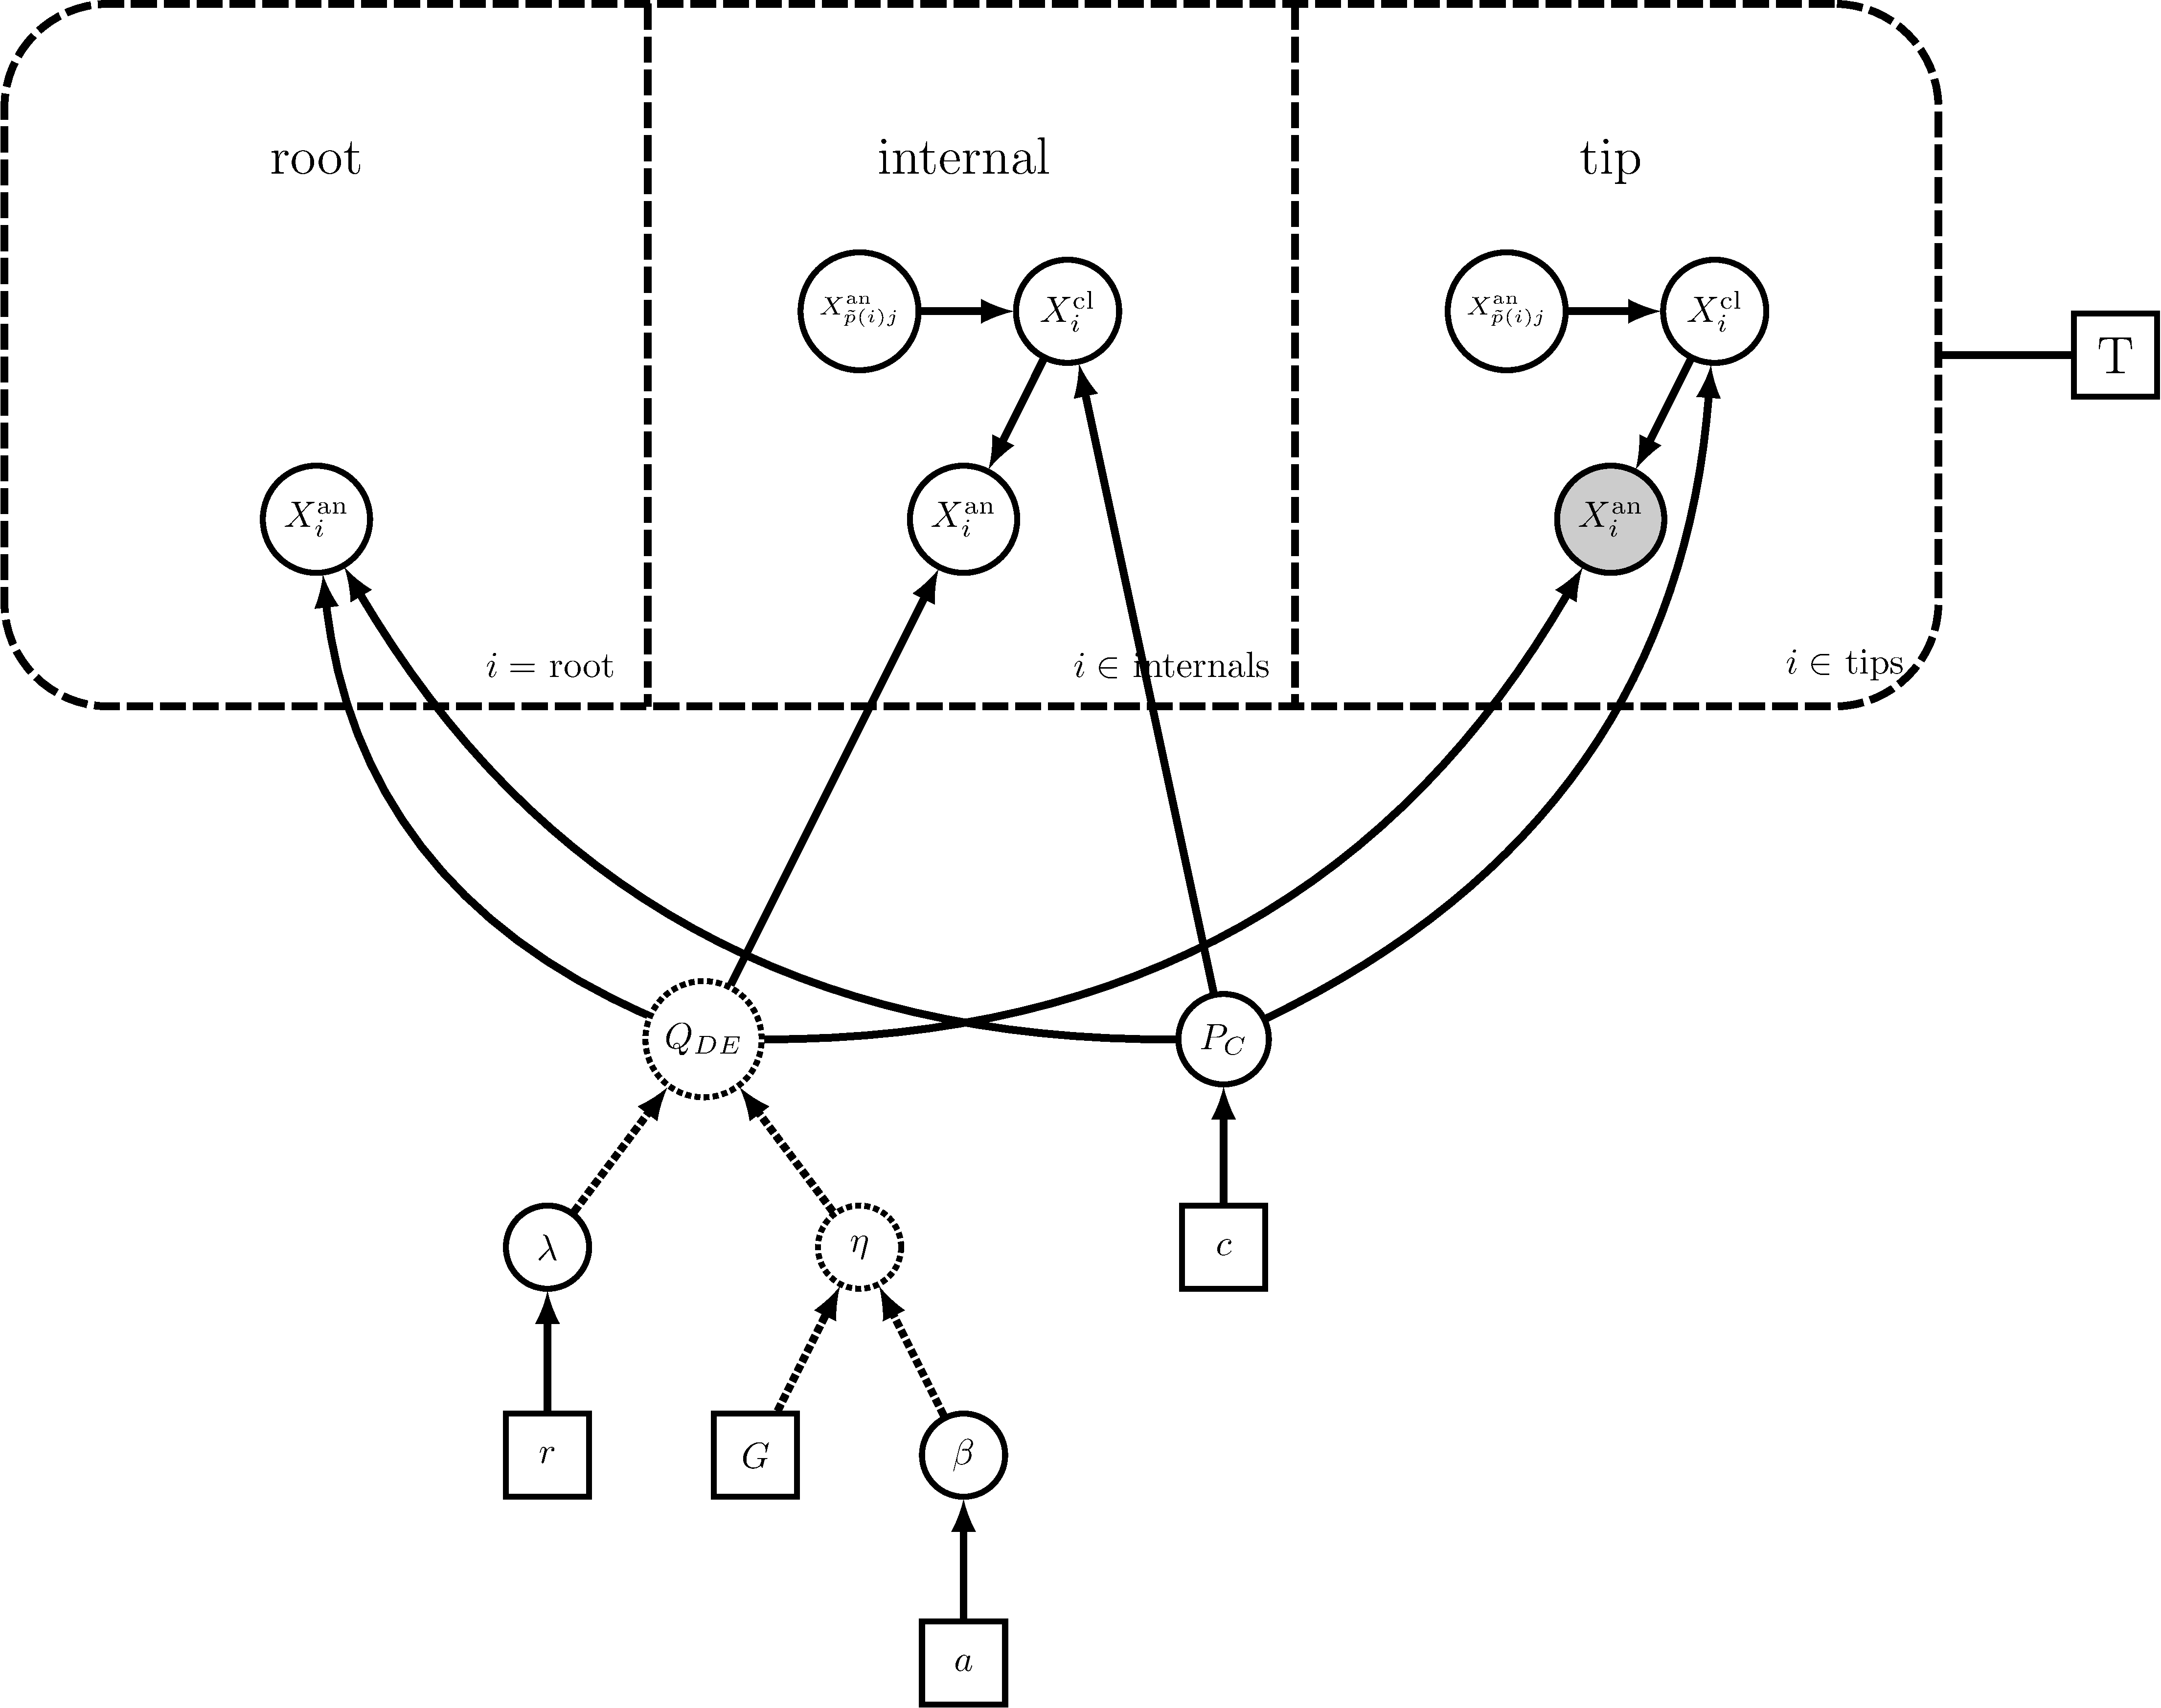
\includegraphics[width=5in]{../RB_Biogeography_Tutorial/figures/bg_dec_dag}
\caption{Graphical model of DEC. The tree plate's topology is fixed by $T$, where each internal node has both an anagenic and cladogenic random variable ($X_i^{\text{an}}$ and $X_i^{\text{cl}}$, resp.) that represents an ancestral species before and after it speciated. Anagenic change is modeled by a continuous time Markov process, where $Q_{DE}$ is the instantaneous rate matrix of area gain and loss, as parameterized by $\lambda$. The geographic distance rate modifier function, $\eta$, takes in the geographical distances and strata as $G$, and the distance power parameter, $\beta$. Cladogenic change is modeled by $P_C$, a Dirichlet-distributed simplex with a flat prior.}
\end{figure}

Let's consider what happens to the size of \textbf{Q} when the number of areas, $N$, becomes large.
For three areas, \textbf{Q} is size $8 \times 8$.
For ten areas, \textbf{Q} is size $1024 \times 1024$, which approaches the largest size matrix that can be exponentiated in a practical amount of time.
This is problematic, meaning we need an alternative method to integrate over historical range evolution events.

You may wonder why matrix exponentiation works fine for molecular substitution models and large multiple sequence alignments.
Molecular substitution models typically assume each site in the multiple sequence alignment evolves independently, which may be justified because recombination degrades linkage disequilibrium over geological timescales.
Conveniently, this keeps \textbf{Q} small even for datasets with many sites.

Remember matrix exponentiation integrates over all \textit{unobserved} transition events during time $t$.
The likelihood of beginning in character $i$ and ending in character $j$ can be computed easily when the explicit series of event types and times are known.
While we will never know the exact history of events, we can use stochastic mapping in conjunction with Markov chain Monte Carlo (MCMC) to repeatedly sample range evolution histories that are consistent with the ranges observed in the study taxa at the tips of the phylogeny.
This technique is an adaptation of the data-augmented phylogenetic method first described by \citet{robinson03}, and was first applied to tertiary structure-dependent evolution of protein-coding nucleotide sequences.

This is the strategy we will use to infer the posterior distribution approximated is 
\newline{Prob$\left( \textbf{X}_{aug}, \theta \mid \textbf{X}_{obs}, T, M \right)$}, where $\textbf{X}_{obs}$ is the range data observed at the tips, $\textbf{X}_{aug}$ is the distribution of ancestral range reconstructions over the phylogeny, $T$, where $\textbf{X}_{aug}$ is inferred jointly with the parameters, $\theta$, assuming the range evolution model, $M$, that describes $\textbf{Q}$ above.
Ancestral range reconstructions are often of primary interest in phylogenetic biogeographic analyses, which are generated with support values as a by-product of the MCMC analysis.

The rest of this tutorial will describe how to assemble the input, run the analysis, assess the output, and visualize the results.

\newpage

%%%%%%%%%%%%%%%%
%%%%%%%%%%%%%%%%
\section{Input}

For this tutorial, we'll use a dataset for 19 species of $Psychotria$ whose range spans the Hawaiian archipelago.
The dataset was originally reported in \citet{nepokroeff03} and analyzed using the maximum likelihood method, LAGRANGE, by \citet{ree08}.
We'll use this dataset for three reasons.
First, it is relatively small, meaning we can produce results quickly.
Second, the Hawaiian archipelago can be broken into naturally discrete areas and has a well-characterized geographical history that is uncomplicated to model.
Third, it has previously been analyzed, which provides some basis for comparison to other methods.
To simplify things, this model will assume we live in a gentler world where presence-absence characters are known without error.

For larger datasets to play with, see {\tt input/sim\_aus\_50tip\_33area.*} for a simulated model where all cladogenic events were sympatric (wide and narrow only). 

\subsection{Nexus file}

The data file contains a matrix of binary characters corresponding to the observed ranges of the study taxa.

%\noindent \\ \impmark  Open the file \texttt{examples/psychotria\_range.txt}.

\begin{framed}
\begin{lstlisting}
#NEXUS

begin data;
  dimensions ntax=19 nchar=4;
  format datatype=standard symbols = "01";
  matrix
    P_mariniana_Kokee2  1000
    P_mariniana_Oahu    0100
    ...
    P_hexandra_Oahu     0100
  ;
end;

Begin trees;
	TREE tree1 = ((((((((P_hawaiiensis_WaikamoiL1:0.9656850499,
	P_mauiensis_Eke:0.9656850499):0.7086257935,(P_fauriei2:1.23
	0218511,P_hathewayi_1:1.230218511):0.4440923324):0.17671155
	...
	89):0.4630447802,P_hexandra_Oahu:2.826939991):2.372081244);
End;
\end{lstlisting}
\end{framed}

Range data is stored in standard Nexus format.
In the {\tt data} block, the first line gives the dimensions of the data matrix and the second line indicates we will be using binary characters.
The four characters correspond to areas defined by the geography file (next subsection).
Rows in the {\tt matrix} block correspond to taxa and their range data, while columns give in which areas each taxon is present (1) or absent (0).
For example, taxon {\tt P\_hexandra\_Oahu} is present only in area 2.

The {\tt trees} block gives the tree describing the shared ancestry of the study species.
Because range evolution occurs in units of geological time, the analysis in this tutorial requires a high-quality time-calibrated phylogeny.
This typically requires a multiple sequence alignment over several loci plus fossils for calibration.
Since this data availability is often the limiting factor for which taxa to include for your analysis, it is best to produce the phylogeny first.
Only afterwards should you begin assembling data for your data matrix.
If your phylogeny cannot be calibrated (e.g. it has no fossils) your best alternative is to proceed with a time tree resulting from a divergence time estimation analysis.
For this tutorial, the phylogeny is assumed to contain no uncertainty.

\subsection{Atlas file}

The geography used in this tutorial represents the Hawaiian archipelago.
Beneath Hawaii, currently the largest and youngest island, is a volcanic hotspot that periodically creates new islands.
The ages of these islands are fairly well known, meaning we can model range availability as a function of time.
Following \citet{ree08}, we will lump groups of smaller islands into single areas to simplify the analysis, leaving us with four areas: Hawaii (H), Oahu (O), Maui (M; this includes Molokai and Lanai), and Kauai (K; this includes Niihau).
These areas are modeled have arisen 0.5, 1.9, 3.7, and 5.5 million years ago, respectively.

Although the model will use discrete-state biogeographic ranges, geographical area is naturally continuous.
This means we must impose some discretization upon the geography to designate a set of biogeographically meaningful characters called areas.
Different methods use different criteria for this discretization, so it is best to perform the discretization yourself rather than blindly using the discretization given from a previous study or method (but do blindly use the dataset included in this tutorial).
Some geographies have natural discretizations: for instance, the Hawaiian archipelago forms naturally discrete areas on the basis of islands.
For many geographies, however, it may unclear how to perform this discretization.
Much like morphological analyses, you might choose to choose areas based on expert opinion, based on some model, or using some ``naive'' uniform discretization.
This procedure is not part of the tutorial, but you should be aware that area definitions are not always obvious or objective.


\newpage

%\noindent \\ \impmark  Open the file \texttt{examples/hawaii\_dynamic.atlas.txt}.

\begin{framed}
%\begin{lstlisting}[basicstyle=\tiny \listingsfont, columns=texcl]
\begin{lstlisting}
{
	"name":"HawaiianArchipelago5my",
	"epochs": [
		{
			"name":"epoch1",
			"start_age":100.0,
			"end_age":3.7,
			"areas":
			[{ "name":"Kauai",  "latitude":19.5667, "longitude": -155.5000, "dispersalValues": [ 1,0,0,0 ] },
			{ "name": "Oahu",   "latitude":19.5667, "longitude": -155.5000, "dispersalValues": [ 0,0,0,0 ] },
			{ "name": "Maui",   "latitude":19.5667, "longitude": -155.5000, "dispersalValues": [ 0,0,0,0 ] },
			{ "name": "Hawaii", "latitude":19.5667, "longitude": -155.5000, "dispersalValues": [ 0,0,0,0 ] }]
		},
		{
			"name":"epoch2",
			...
		},
		{
			"name":"epoch3",
			...
		},
		{
			"name":"epoch4",
			"start_age":0.5,
			"end_age":0.0,
			"areas":
			[{ "name":"Kauai",  "latitude":22.0833, "longitude": -159.5000, "dispersalValues": [ 1,1,1,1 ] },
			{ "name": "Oahu",   "latitude":21.4722, "longitude": -157.9772, "dispersalValues": [ 1,1,1,1 ] },
			{ "name": "Maui",   "latitude":20.8000, "longitude": -156.3333, "dispersalValues": [ 1,1,1,1 ] },
			{ "name": "Hawaii", "latitude":19.5667, "longitude": -155.5000, "dispersalValues": [ 1,1,1,1 ] }]
		}
	]
}
\end{lstlisting}
\end{framed}

This is called the Atlas file, which uses a file format called JSON.
JSON is a lightweight format used to assign values to variables in a hierarchical manner.
There are three main tiers to the hierarchy in the Atlas file: the atlas, the epoch, and the area.
In the lowest tier, each area corresponds to a character in the model and is assigned it's own properties.
In the middle tier, each epoch contains the set of homologous areas (characters) that may be part of a species' range, but importantly the properties of these areas may take on different values during different intervals of time, as given by the {\tt start\_age} and {\tt end\_age} variables.
Because the tree and range evolution model also operate on units of geological time, the rates of area gain and loss can condition on areas' properties as a function of time.
Sometimes these models are called stratified models or epochal models.
Finally, the atlas contains the array of epochs in the highest tier.

Each area is assigned a {\tt latitude} and {\tt longitude} to represent its geographical coordinates, ideally the area's centroid.
If a centroid does not represent the distance between areas, splitting the area into multiple smaller areas is reasonable.
The data augmentation approach used in this analysis allows you to use more areas as desired, whereas matrix exponentiation methods are limited to approximately ten areas.
The distance between any two areas' coordinates inform to distance-dependent dispersal parameter ($\beta$ from the $\eta(\cdot)$ function) for range expansion events, so coordinates roughly close to the center of the area suffice.
Here, the {\tt latitude} and {\tt longitude} change in each of the four epochs, where they begin at the current location of Hawaii and drift northwesterly until they reach their current positions.

In addition, each area is marked as habitable or not using the {\tt dispersalValues} array.
The elements in the array correspond to the other areas defined in the analysis.
For example, in {\tt epoch1}, Kauai's {\tt dispersalValues} is equal to {\tt [ 1,0,0,0 ]}, which indicates Kauai exists at that point in time but it is not in contact with any other areas, i.e. the range in that area cannot expand into other areas.
The {\tt dispersalValues} for Oahu, Maui, and Hawaii are all equal to {\tt [ 0,0,0,0 ]}, meaning no species may be present in that area during the time interval of {\t epoch1} during ages from 10.0 to 3.7. In contrast, {\tt epoch4}, from ages 0.5 to the present, range expansions may occur between any pair of areas and any area may be included in a species' range.

\section{RevBayes Analysis}

There are six major parts to the analysis.

First, we need to read in the input files and assign analysis settings.
Second, we need to construct our model.
Third, we need to assign moves and monitors to our model parameters for use with Markov chain Monte Carlo (MCMC).
Fourth, we will run an MCMC analysis assuming a complex model.
Fifth, we will compare the complex model with a simple model using Bayes factors.
Finally, we'll analyze our MCMC output.

\subsection{Analysis settings}

\setlength{\parindent}{0pt}

%\noindent \\ \impmark Open the RevBayes console

\begin{snugshade}
\begin{lstlisting}
$ revbayes
\end{lstlisting}
\end{snugshade}

First, we'll assign all our input files to {\tt String} variables.
\begin{snugshade}
\begin{lstlisting}
RevBayes > in_fp   <- "./input/"
RevBayes > data_fn <- "psychotria_range.nex"
RevBayes > area_fn <- "hawaii_dynamic.atlas.txt"
RevBayes > out_fp  <- "./output/"
RevBayes > out_str <- "bg_2rate"
\end{lstlisting}
\end{snugshade}

Then we'll create our range data, tree, and atlas objects

\begin{snugshade}
\begin{lstlisting}
RevBayes > data  <- readDiscreteCharacterData(in_fp + data_fn)
RevBayes > tree  <- readTrees(in_fp + data_fn)[1]
RevBayes > atlas <- readAtlas(in_fp + area_fn)
\end{lstlisting}
\end{snugshade}

%Verify the data and tree share the same number of taxa and the data and atlas share the same number of characters
%
%\begin{snugshade}
%\begin{lstlisting}
%RevBayes > data.ntaxa() == tree.ntips()
%   true
%RevBayes > data.nchar() == atlas.nareas()
%   true
%\end{lstlisting}
%\end{snugshade}


\subsection{Creating the model}

Here, we will compose our rate matrix, {\bf Q}, parameterized by the transition rates, $\lambda$, and the distance dependent dispersal power parameter, $\beta$.

First, for $\lambda$, we will create a vector of two rates, where {\tt glr[1]} corresponds to the rate of area loss (local extinction) and {\tt glr[2]} corresponds to the rate of area gain (dispersal).
Each rate will be drawn from an exponential distribution with rate 10.0 (mean 0.1).
Because our tree is in units of millions of years, this means our prior expectation is that any given species undergoes one dispersal or extinction event per area per ten million years.

To introduce this to the model, type
\begin{snugshade}
\begin{lstlisting}
RevBayes > for (i in 1:2) glr[i] ~ dnExponential(10.0)
\end{lstlisting}
\end{snugshade}

Next, we will create {\tt dp}, which determines the importance of geographical distance to dispersal.
Remember that values of $\beta$ far from zero means distance is important.
So, if we we assign a prior that pulls $\beta$ towards zero, then posterior values of $\beta$ far from zero indicate the range data are informative of the importance of distance to dispersal.
We'll use an exponential distribution with rate 10.0 (mean 0.1) as a prior for {\tt dp}.

We will also create a deterministic node to modify the rate of dispersal between areas by evaluating {\tt dp} and {\tt atlas}.
This node is determined by the function {\tt fnBiogeoGRM}, where GRM stands for ``geographical rate modifier'', and plays the role of the $\eta(\cdot)$ rate-modifier function mentioned earlier.
We will tell the {\tt fnBiogeoGRM} function to modify dispersal rates based on distances and whether or not the area exists during an epoch.

\begin{snugshade}
\begin{lstlisting}
RevBayes > dp ~ dnExponential(10.0)
RevBayes > grm := fnBiogeoGRM(atlas=atlas, distancePower=dp, useAvailable=true, useDistance=true)
\end{lstlisting}
\end{snugshade}

Now we need a deterministic node to represent the rate matrix, {\bf Q}.
To determine the value of this node, we'll use the function {\tt fnBiogeoDE} to assign our model parameters to transition rates as described in the introduction.
As input, we'll pass our gain and loss rates, {\tt glr}, and our geographical rate modifier, {\tt grm}.
In addition, we'll inform the function of the number of areas in our analysis and whether we will allow species to be absent in all areas (i.e. have the null range).

\begin{snugshade}
\begin{lstlisting}
RevBayes > Q := fnBiogeoDE(gainLossRates=glr, geoRateMod=grm, numAreas=4, forbidExtinction=true)
\end{lstlisting}
\end{snugshade}

To extract information for the frequencies of different cladogenic event types, we will create a Dirichlet-distributed stochastic node.
The simplex is over three events, subset sympatry (index 0), allopatry (index 1), and widespread sympatry (index 2), but not over narrow sympatry whose range size is one.
The prior parameter {\tt [1,1,1]} is known as a flat prior, meaning all event types are expected to occur at equal frequency.
If there is information in the data of a dominant cladogenic mode of range evolution, the posterior simplex values in {\tt csf} will reflect this.

\begin{snugshade}
\begin{lstlisting}
RevBayes > csf ~ dnDirichlet([1,1,1])
\end{lstlisting}
\end{snugshade}

For the model's final node, we create the stochastic node for the continuous-time Markov chain (CTMC).
This node's distribution is {\tt dnPhyloDACTMC} where {\tt DA} indicates the CTMC uses data-augmentation to compute the likelihood rather than Felsenstein's pruning algorithm.
To create the distribution, we must pass it our {\tt tree} and {\tt Q} objects, but additionally inform the distribution that it will be using a biogeographic model, that it will introduce the simple cladogenic range evolution events described in \citet{ree08} ({\tt useCladogenesis=true}), and that it will assign zero probability to a transition away from the null range state.

\begin{snugshade}
\begin{lstlisting}
RevBayes > M ~ dnPhyloDACTMC(tree=tree, Q=Q, C=csf, type="biogeo", forbidExtinction=true, useCladogenesis=true)
\end{lstlisting}
\end{snugshade}

So we may evaluate the graphical model's likelihood, we tell the CTMC to observe the {\tt data} object, which will prime the model with data-augmented character histories.
Now {\tt M} has a defined likelihood value.
\begin{snugshade}
\begin{lstlisting}
RevBayes > M.clamp(data)
RevBayes > M.lnProb
   -56.0288
\end{lstlisting}
\end{snugshade}

Finally, we encapsulate our graphical model into a {\tt Model} object, which can learn the model's structure and dependencies from any model parameter.
\begin{snugshade}
\begin{lstlisting}
RevBayes > my_model <- model(glr)
\end{lstlisting}
\end{snugshade}

\subsection{Running an MCMC analysis}

Now that we have our {\tt Model} object, we can soon run an MCMC analysis.
Remember that MCMC approximates the posterior distribution by repeatedly proposing new model parameter values, accepting or rejecting those new parameter values based on the model likelihood (and on biases in the proposal distribution), then reporting the sampled parameter values.

First, let's assign moves to our model parameters.
These parameters are all supported for real positive values, which is appropriate for use with scale-multipler proposal, {\tt mvScale()}.
To inspect our model parameter types and the proposal argument types, enter

\begin{snugshade}
\begin{lstlisting}
RevBayes > type(dp)
   RealPos
RevBayes > type(glr)
   RealPos[]
RevBayes > mvScale
   Move_Scale function (RealPos x, RealPos lambda, Bool tune, RealPos weight)
\end{lstlisting}
\end{snugshade}

The arguments for {\tt mvScale} are fairly typical as far as RevBayes {\tt Move} objects go: {\tt x} is the stochastic node the {\tt Move} will update, {\tt lambda} is proportional to how radically different proposed parameter values will tend to be, {\tt tune} allows {\tt lambda} to be adjusted automatically as the MCMC runs, and {\tt weight} tells the MCMC how many times to perform the {\tt Move} during a single MCMC generation (e.g., {\tt weight=2.0)} means each generation will call that {\tt Move} for the parameter {\tt x} twice).


\begin{snugshade}
\begin{lstlisting}
RevBayes > moves[1] <- mvScale(x=glr[1], lambda=0.5, tune=false, weight=5.0)
RevBayes > moves[2] <- mvScale(x=glr[2], lambda=0.5, tune=false, weight=5.0)
RevBayes > moves[3] <- mvScale(x=dp, 	 lambda=0.5, tune=false, weight=5.0)
RevBayes > moves[4] <- mvSimplexElementScale(csf, alpha=10.0, tune=false, weight=4.0)
\end{lstlisting}
\end{snugshade}

In addition to proposing new model parameter values, we must also propose new data-augmented states and events to properly integrate over the space of possible range histories.
The major challenge to sampling character histories is ensuring the character histories are consistent with the observations at the tip of the tree.
The proposals in this tutorial use \citet{nielsen02}'s rejection sampling algorithm, with some modifications to account for cladogenic events and epoch-based rate matrices.

The basic idea is simple.
Each time a character history proposal is called, it selects a node at random from the tree.
Path history proposals ({\tt mvPathCHRS()}) propose a new character history for the lineage leading to that node.
Node history proposals ({\tt mvNodeCHRS()}) propose a new character history for the node and for the three lineages incident to that node.
The character history proposal also samples some number of areas to update, ranging from one to all of the areas.
Once the new character history is proposed, the likelihood of the model is evaluated and the MCMC accepts or rejects the new state according to e.g. the Metropolis-Hastings algorithm.

Because these {\tt Move} objects update the character histories stored in the data-augmented CTMC node, e.g. {\tt M},
they require access to a {\tt TimeTree} object to know which lineages are sisters and whether the lineages span various epochs, and a {\tt RateMap\_Biogeography} object to propose new character histories.
The {\tt lambda} argument gives what proportion of areas' character histories to update.
Here, if {\tt lambda=0.2}, then the proposal will redraw character histories for each area with probability 0.2 (in addition to one random area with probability 1).
Below, we use two moves of each type with {\tt lambda=0.2} and {\tt lambda=1.0} for partial and full character history updates, respectively.
Indicating {\tt type="biogeo"} informs the {\tt Move} object to be aware of special character history constraints, such as cladogenic events and forbidden null ranges.
The {\tt weight} parameter should be assigned a value proportional to the number of nodes in the analysis to ensure proper mixing.

Let's create the character history moves as follows.

\begin{snugshade}
\begin{lstlisting}
RevBayes > n_nodes  <- tree.nnodes()
RevBayes > moves[5] <- mvNodeCHRS(ctmc=M, qmap=Q, tree=tree, lambda=0.2, type="biogeo", weight=2.0*n_nodes)
RevBayes > moves[6] <- mvPathCHRS(ctmc=M, qmap=Q, tree=tree, lambda=0.2, type="biogeo", weight=2.0*n_nodes)
RevBayes > moves[7] <- mvNodeCHRS(ctmc=M, qmap=Q, tree=tree, lambda=1.0, type="biogeo", weight=n_nodes)
RevBayes > moves[8] <- mvPathCHRS(ctmc=M, qmap=Q, tree=tree, lambda=1.0, type="biogeo", weight=n_nodes)
\end{lstlisting}
\end{snugshade}

Now that we have moves for all our parameters and the character histories, we'll proceed with assigning {\tt Monitor} objects to record their values.
The first two {\tt Monitor} objects are fairly standard and found in most RevBayes MCMC analyses.
{\tt mnScreen} reports the values for any nodes assigned to {\tt RevObject ...} every {\tt printgen} generations to the terminal screen.
{\tt mnModel} reports the values for all nodes in the {\tt Model} object every {\tt printgen} generations to the file assigned to {\tt filename}, which is delimited by the {\tt separator} character.

\begin{snugshade}
\begin{lstlisting}
RevBayes > mnScreen
   Mntr_Screen function (RevObject ..., Natural printgen, Bool posterior, Bool
   likelihood, Bool prior)
RevBayes > monitors[1] <- mnScreen(printgen=10, glr, dp, csf)
RevBayes > mnModel
   Mntr_Model function (String filename, Natural printgen, String separator,
   Bool posterior, Bool likelihood, Bool prior, Bool append, Bool
   stochasticOnly)
RevBayes > monitors[2] <- mnModel(filename=out_fp+params_fn, printgen=10)
\end{lstlisting}
\end{snugshade}

Like any parameter, we can sample the augmented range histories from the MCMC to approximate the posterior distribution of range histories.
This is statistically equivalent to generating ancestral state reconstructions from a posterior distribution via stochastic mapping.
We will extract these reconstructions using special monitors designed for the {\tt dnPhyloDACTMC} distribution.

Next, we will create {\tt Mntr\_CharacterHistoryNewickFile} objects to record the sampled character history states for each node in the tree.
This {\tt Monitor} has two {\tt style} options: {\tt counts} reports the number of gains and losses per branch in a tab-delimited Tracer-readable format;  {\tt events} reports richer information of what happens along a branch, anagenically and cladogenically, using an extended Newick format.
How to read these file formats will be discussed in more detail in Section \ref{sec:posterior}.

\begin{snugshade}
\begin{lstlisting}
RevBayes > mnCharHistoryNewick
   Mntr_CharacterHistoryNewickFile function (String filename,
   AbstractCharacterData ctmc, TimeTree tree, Natural printgen, String
   separator, Bool posterior, Bool likelihood, Bool prior, Bool append, String
   style = events|counts
   , String type = biogeo
   )
RevBayes > monitors[3] <- mnCharHistoryNewick(filename=fp+out_str+".events.txt", ctmc=M, tree=tree, printgen=100, style="events")
RevBayes > monitors[4] <- mnCharHistoryNewick(filename=fp+out_str+".counts.txt", ctmc=M, tree=tree, printgen=100, style="counts")
\end{lstlisting}
\end{snugshade}

As our last monitor, the {\tt Mntr\_CharacterHistoryNhxFile} records character history values throughout the MCMC analysis, then stores some simple posterior summary statistics as a Nexus file.
These summary statistics could be computed from the previously mentioned {\tt Monitor} output files, but {\tt mnCharHistoryNhx} provides a simple way to produce Phylowood-compatible files.
We will also discuss this file's format in more detail later in the tutorial.

\begin{snugshade}
\begin{lstlisting}
RevBayes > mnCharHistoryNhx
   Mntr_CharacterHistoryNhxFile function (String filename, AbstractCharacterData
   ctmc, TimeTree tree, RlAtlas atlas, Natural samplegen, Natural maxgen,
   Probability burnin, String separator, Bool posterior, Bool likelihood, Bool
   prior, String type = biogeo
   )
RevBayes > monitors[5] <- mnCharHistoryNhx(filename=fp+out_str+".nhx.txt", ctmc=M, tree=tree, atlas=atlas, samplegen=100, maxgen=25000, burnin=0.2)
\end{lstlisting}
\end{snugshade}

Before we run the MCMC, we'd like to get the node index of the ancestor 
When analysing the output, we'll take some special interest in the branch for the most recent common ancestor of {\it P. kaduana} and {\it P. hatheway}.
We will identify this lineage by its index, 23, which is meaningful only for a fixed tree topology,
\begin{snugshade}
\begin{lstlisting}
RevBayes > names = tree.names()
RevBayes > names[15]
   P_kaduana_PuuKukuiAS
RevBayes > names[16]
   P_hathewayi_1
RevBayes > mrcaIndex(tree=tree,clade=clade(names[15],names[16]))
   23
\end{lstlisting}
\end{snugshade}


\subsection{Running an MCMC analysis}

Now all that's left is to configure and run our MCMC analysis.
For this, we create an {\tt Mcmc} object, which we give our {\tt Move} vector, our {\tt Monitor} vector, and our {\tt Model object}

\begin{snugshade}
\begin{lstlisting}
RevBayes > mcmc
   MCMC function (Model model, Monitor[] monitors, Move[] moves, String
   moveschedule = sequential|random|single
   )
RevBayes > my_mcmc <- mcmc(my_model, monitors, moves)
\end{lstlisting}
\end{snugshade}

MCMC typically requires some period of burn-in before it reaches stationarity, i.e. from a random starting point, it takes some time for the chain to produce valid samples from the posterior distribution.
By running {\tt burnin()}, we tell the {\tt Mcmc} object to propose and reject new states but {\it not} to record anything to file.
After burn-in is complete, we call {\tt run()}, where we begin recording valid posterior samples under our model.

\begin{snugshade}
\begin{lstlisting}
RevBayes > my_mcmc.burnin(generations=1000, tuningInterval=50)
RevBayes > my_mcmc.run(generations=25000)
\end{lstlisting}
\end{snugshade}

Everything we've done is contained in the file {\tt biogeography\_DEC\_2rate.Rev}.
You can modify this file as you like then re-run the analysis by typing

\begin{snugshade}
\begin{lstlisting}
RevBayes > source("./scripts/biogeography_DEC_2rate.Rev")
\end{lstlisting}
\end{snugshade}

\subsection{Model selection using Bayes factors}

Bayes factors (BFs) are used to select which of two models better describes the observed data, $\mathbf{X}_{obs}$, and are computed as the ratio of marginal likelihoods for those two models.
One might prefer to analytically compute the marginal likelihood, but it's the same intractable quantity we intentionally avoid computing when using MCMC in a Bayesian context.
Instead, we must estimate the marginal likelihood from our posterior distribution samples.
Here, we will use thermodynamic integration \citep{lartillot06} and stepping-stone approximation \citep{xie10}.
The exact details of these techniques will not be covered here, but there is an important practical point to mention: both methods rely on computing a number of ``power posterior'' distributions.
Computing more power posteriors increases the marginal likelihood estimator's accuracy at the cost of computational time.

Moving on, we'll compute the Bayes factor to compare a simple one-rate model, which asserts the rate of area gain and loss are always equal, to a two-rate model which allows these rates to vary independently.
Rather than specifying the model manually, we will load (source) the model definition from a file then enter the commands to compute its marginal likelihood.
For faster results, we will use two separate RevBayes sessions, one for each model.
For each session, the power posterior analysis run for 1000 generations during burn-in then 1000 generations per each of 30 power posterior categories.

First session:
\begin{snugshade}
\begin{lstlisting}
RevBayes > source("./scripts/biogeography_DEC_1rate.Rev")
RevBayes > pp_fn <- out_fp + out_str + ".pp.txt"
RevBayes > pow_p <- powerPosterior(my_model, moves, pp_fn, cats=30) 
RevBayes > pow_p.burnin(generations=1000,tuningInterval=100)
RevBayes > pow_p.run(generations=5000)
\end{lstlisting}
\end{snugshade}

Second session:
\begin{snugshade}
\begin{lstlisting}
RevBayes > source("./scripts/biogeography_DEC_2rate.Rev")
RevBayes > pp_fn <- out_fp + out_str + ".pp.txt"
RevBayes > pow_p <- powerPosterior(my_model, moves, pp_fn, cats=30) 
RevBayes > pow_p.burnin(generations=1000,tuningInterval=100)
RevBayes > pow_p.run(generations=5000)  
\end{lstlisting}
\end{snugshade}

Each power posterior analysis will write their contents to the file given in {\tt pp\_fn}.
These files are {\tt bg\_1rate.pp.txt} and {\tt bg\_2rate.pp.txt} for the simple and complex models, respectively.
This may take a few minutes.
When complete, the power posterior files may then be used to compute marginal likelihoods.
For example, from the RevBayes session analyzing the simple one-rate model

\begin{snugshade}
\begin{lstlisting}
RevBayes > ss <- steppingStoneSampler(file=pp_fn)
RevBayes > ss.marginal() 
RevBayes > ps <- pathSampler(file=pp_fn)
RevBayes > ps.marginal() 
\end{lstlisting}
\end{snugshade}

For a given model, the path sampling and stepping stone sampling methods should produce similar marginal likelihood estimates.
Values should be within one log likelihood unit of one another.
If the values are extremely different, this may indicate {\tt powerPosterior} should be re-run with a larger number of {\tt cats}.
We chose {\tt cats=30} which should suffice, and we see no problem.
Then from the complex two-rate model RevBayes session using the same commands as above.
Finally, we can compute the Bayes factor, which is simply the ratio of marginal likelihoods.

\begin{snugshade}
\begin{lstlisting}
RevBayes > exp(-51.7202)/exp(-52.3158)
   1.81412
\end{lstlisting}
\end{snugshade}

A value of one would mean both models had equal marginal likelihoods.
A value less than one would indicate the first model, the simple model, had a larger marginal likelihood, and was therefore favored by model testing.
But that's not the case, the value is greater than one, and the complex two-rate model is favored.
Similar to frequentist interpretations of significance for p-values, there is no universal and objective criterion of significance with Bayes factors, but most would agree a factor of 1.8 (or 1.0/1.8) indicates weak support for one model over the other.

\section{Output}

\subsection{Sampled parameters from {\tt ScreenMonitor}}

The {\tt mnScreen} monitor reports model parameter values to the screen, where each row corresponds to the current accepted MCMC state, and each column reports some model feature, such as the model likelihood or a parameter value.
Every 20 iterations, this monitor re-prints the column headers.

\begin{snugshade}
%\begin{lstlisting}[basicstyle=\tiny \listingsfont, columns=texcl]
\begin{lstlisting}
RevBayes > my_mcmc.run(generations=25000)

Running MCMC simulation for 25000 iterations
The simulator uses 8 different moves in a random
move schedule with 241 moves per iteration

Iteration   |   Posterior  |          dp  |      glr[1]  |      glr[2]  |      csf[1]  |      csf[2]  |      csf[3]
-------------------------------------------------------------------------------------------------------------------
0           |    -51.3307  |   0.0570518  |    0.175137  |   0.0580957  |    0.330891  |    0.255308  |    0.413801
10          |    -54.4257  |   0.0416423  |    0.166936  |    0.178402  |   0.0549136  |    0.148854  |    0.796233
20          |    -58.0696  |   0.0991853  |    0.136495  |    0.122135  |    0.308418  |    0.448892  |    0.242689
30          |    -46.5049  |     0.10676  |   0.0958918  |   0.0959592  |    0.543837  |    0.363871  |   0.0922922
40          |    -42.8697  |    0.173549  |    0.158565  |   0.0662419  |    0.569416  |    0.126439  |    0.304145
50          |    -43.5319  |    0.117868  |    0.196497  |   0.0523307  |    0.440269  |    0.257171  |     0.30256

...
\end{lstlisting}
\end{snugshade}

For the complex 2-rate model, our model parameters are {\tt dp}, the distance power parameter, and the rates of area loss and gain, {\tt glr[1]} and {\tt glr[2]}, respectively, and the frequencies for subset sympatry, allopatry, and widespread sympatry {\tt csf[1]}, {\tt csf[2]}, and {\tt csf[3]}, respectively. 
If you notice the value of some parameter is rarely updated from iteration to iteration, the MCMC is probably mixing poorly therefore it's not generating samples from the posterior distribution (the MCMC's stationary distribution).
In this case, you may want to re-run the analysis with different arguments for the {\tt Move} object assigned to that parameter.

\subsection{Sampled parameters from {\tt ModelMonitor}}

This tab-delimited file contains parameter samples from the posterior distribution.
As with the {\tt ScreenMonitor}, columns are model or parameter values and rows are MCMC cycles.

\begin{framed}
%\begin{lstlisting}[basicstyle=\tiny \listingsfont, columns=texcl]
\begin{lstlisting}
Iteration  Posterior  Likelihood    Prior  glr[1]  glr[2]  dp  csf[1]  csf[2]  csf[3]
0           -51.3307    -56.0288  4.69806  0.175137  0.0580957  0.057051  0.330891  0.255308  0.413801
10          -54.4257    -58.1568  3.73110  0.166936  0.1784020  0.041642  0.054913  0.148854  0.796233
20          -58.0696    -62.0923  4.02274  0.136495  0.1221350  0.099185  0.308418  0.448892  0.242689
30          -46.5049    -51.1197  4.61480  0.095891  0.0959592  0.106760  0.543837  0.363871  0.092292
40          -42.8697    -46.4870  3.61735  0.158565  0.0662419  0.173549  0.569416  0.126439  0.304145
50          -43.5319    -47.4659  3.93394  0.196497  0.0523307  0.117868  0.440269  0.257171  0.302560

...
\end{lstlisting}
\end{framed}

%\noindent \\ \impmark Open Tracer, select the fields for the posterior probability and area gain rate, {\tt glr[2]}, then click the Joint-Marginal tab.

\begin{figure}[H]
\centering
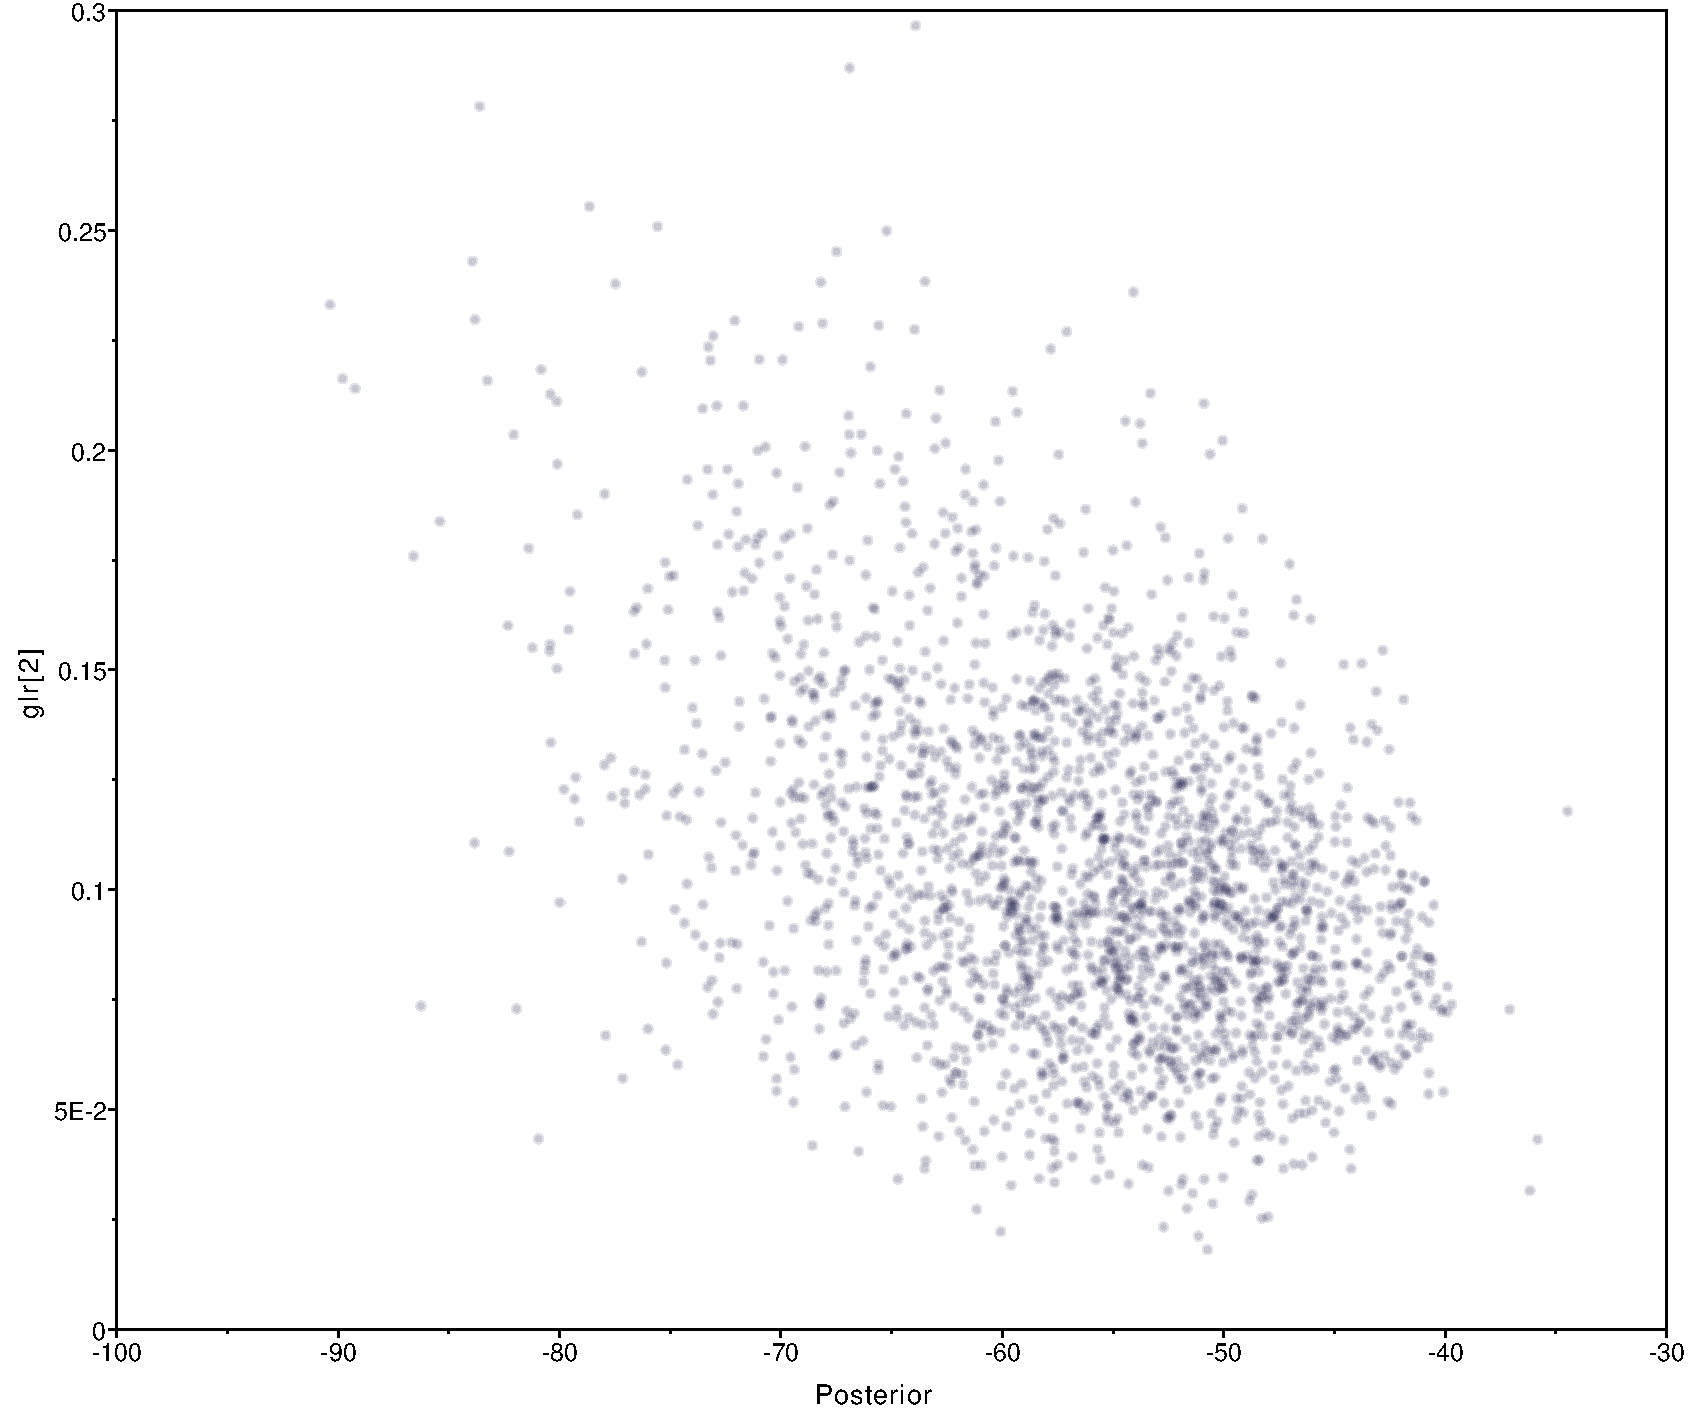
\includegraphics[width=3in]{../RB_Biogeography_Tutorial/figures/joint_rgain_posterior}
\caption{Joint-marginal distribution of posterior and area gain rate, $\lambda_1$.}
\end{figure}

Here, we see a strong negative correlation between the posterior probability and the area gain rate, which is expected.
Next, click the Estimates tab then select the three {\tt csf} parameters.

\begin{figure}[H]
\centering
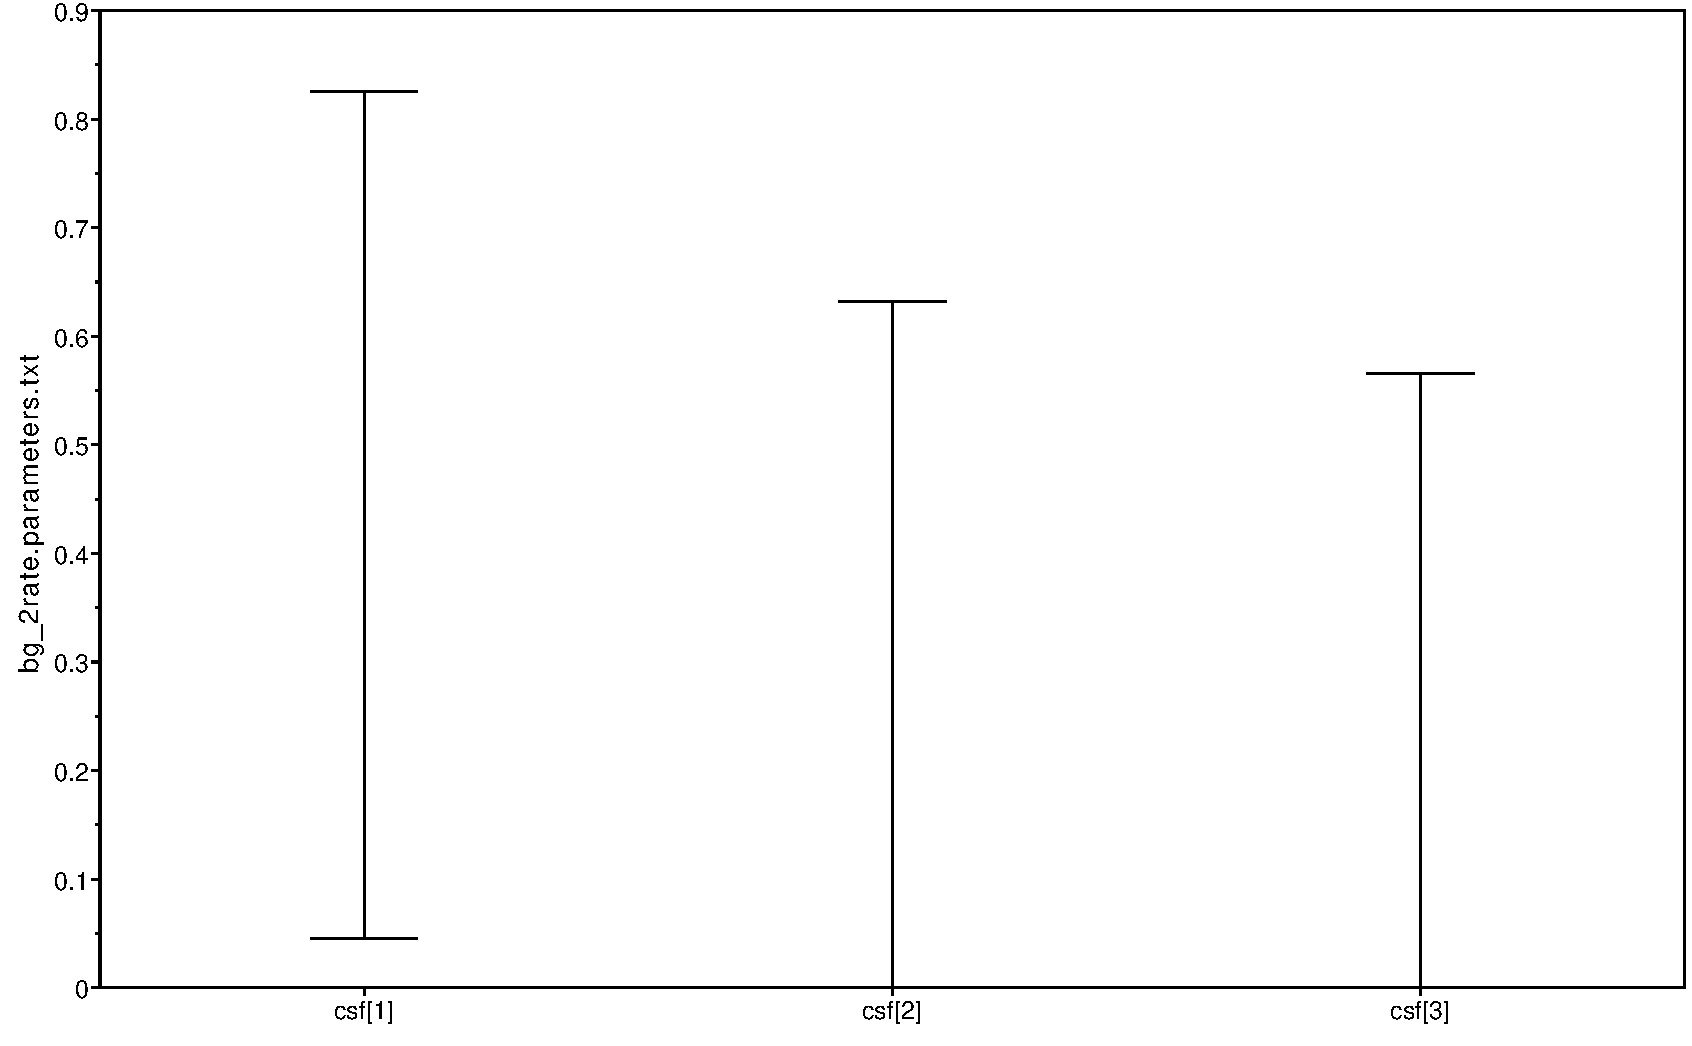
\includegraphics[width=3in]{../RB_Biogeography_Tutorial/figures/clado_freq_posterior}
\caption{Mean values for the cladogenic state frequency simplex, where {\tt csf[1]}, {\tt csf[2]}, and {\tt csf[3]} correspond to subset sympatry, allopatry, and wide sympatry whose mean posterior values are 0.45, 0.30, and 0.25, respectively.}
\end{figure}


\subsection{Biogeographic event counts from {\tt mnCharHistoryNewick}}

Recording stochastic mappings in a Tracer-compatible format requires some summarization.
This monitor generates a tab-delimited file where the number of events of each type for each branch is recorded.

%\noindent \\ \impmark Open {\tt ./output/bg\_2rate.counts.txt} in a text editor.

\begin{framed}
%\begin{lstlisting}[basicstyle=\tiny \listingsfont, columns=texcl]
\begin{lstlisting}
Iteration  Posterior  Likelihood    Prior	t_s0	t_s1	t_c0	t_c1	t_c2	t_c3	b0_s0	b0_s1	b0_c	...
0           -51.3307    -56.0288  4.69806	9	9	18	0	0	0	1	1	0	...	
10          -54.4257    -58.1568  3.73110	9	10	17	0	0	1	1	1	0	...
20          -58.0696    -62.0923  4.02274	11	9	15	2	1	0	2	1	1	...
30          -46.5049    -51.1197  4.61480	8	8	18	0	0	0	1	1	0	...
40          -42.8697    -46.4870  3.61735	7	7	18	0	0	0	1	1	0	...
50          -43.5319    -47.4659  3.93394	7	7	18	0	0	0	1	1	0	...
...
\end{lstlisting}
\end{framed}

For example, {\tt b2\_s1} gives the number of areas that are gained for the branch leading to the node indexed 2.
{\tt b2\_c} gives the cladogenic event type that gives rise to the node indexed 2, where narrow sympatry, subset sympatry, allopatry, and widespread sympatry are recorded as {\tt 0}, {\tt 1}, {\tt 2}, and {\tt 3}, respectively. The columns {\tt t\_s0} and {\tt t\_s1} give the sum of events over all branches. {\tt t\_c0}, {\tt t\_c1}, and {\tt t\_c2} give the total number of narrow sympatric, subset sympatric, allopatric, and widespread sympatric cladogenic events over the entire tree.

Because the expected number of gain events should be proportional to the area gain rate, we expect to see the same negative correlation between posterior probability and number of events as we did with the posterior and rate in the {\tt parameters.txt} file.

Open Tracer, select the fields for the posterior probability and the number of gained areas over the tree, {\tt t1}, then click the Joint-Marginal tab.

\begin{figure}[H]
\centering
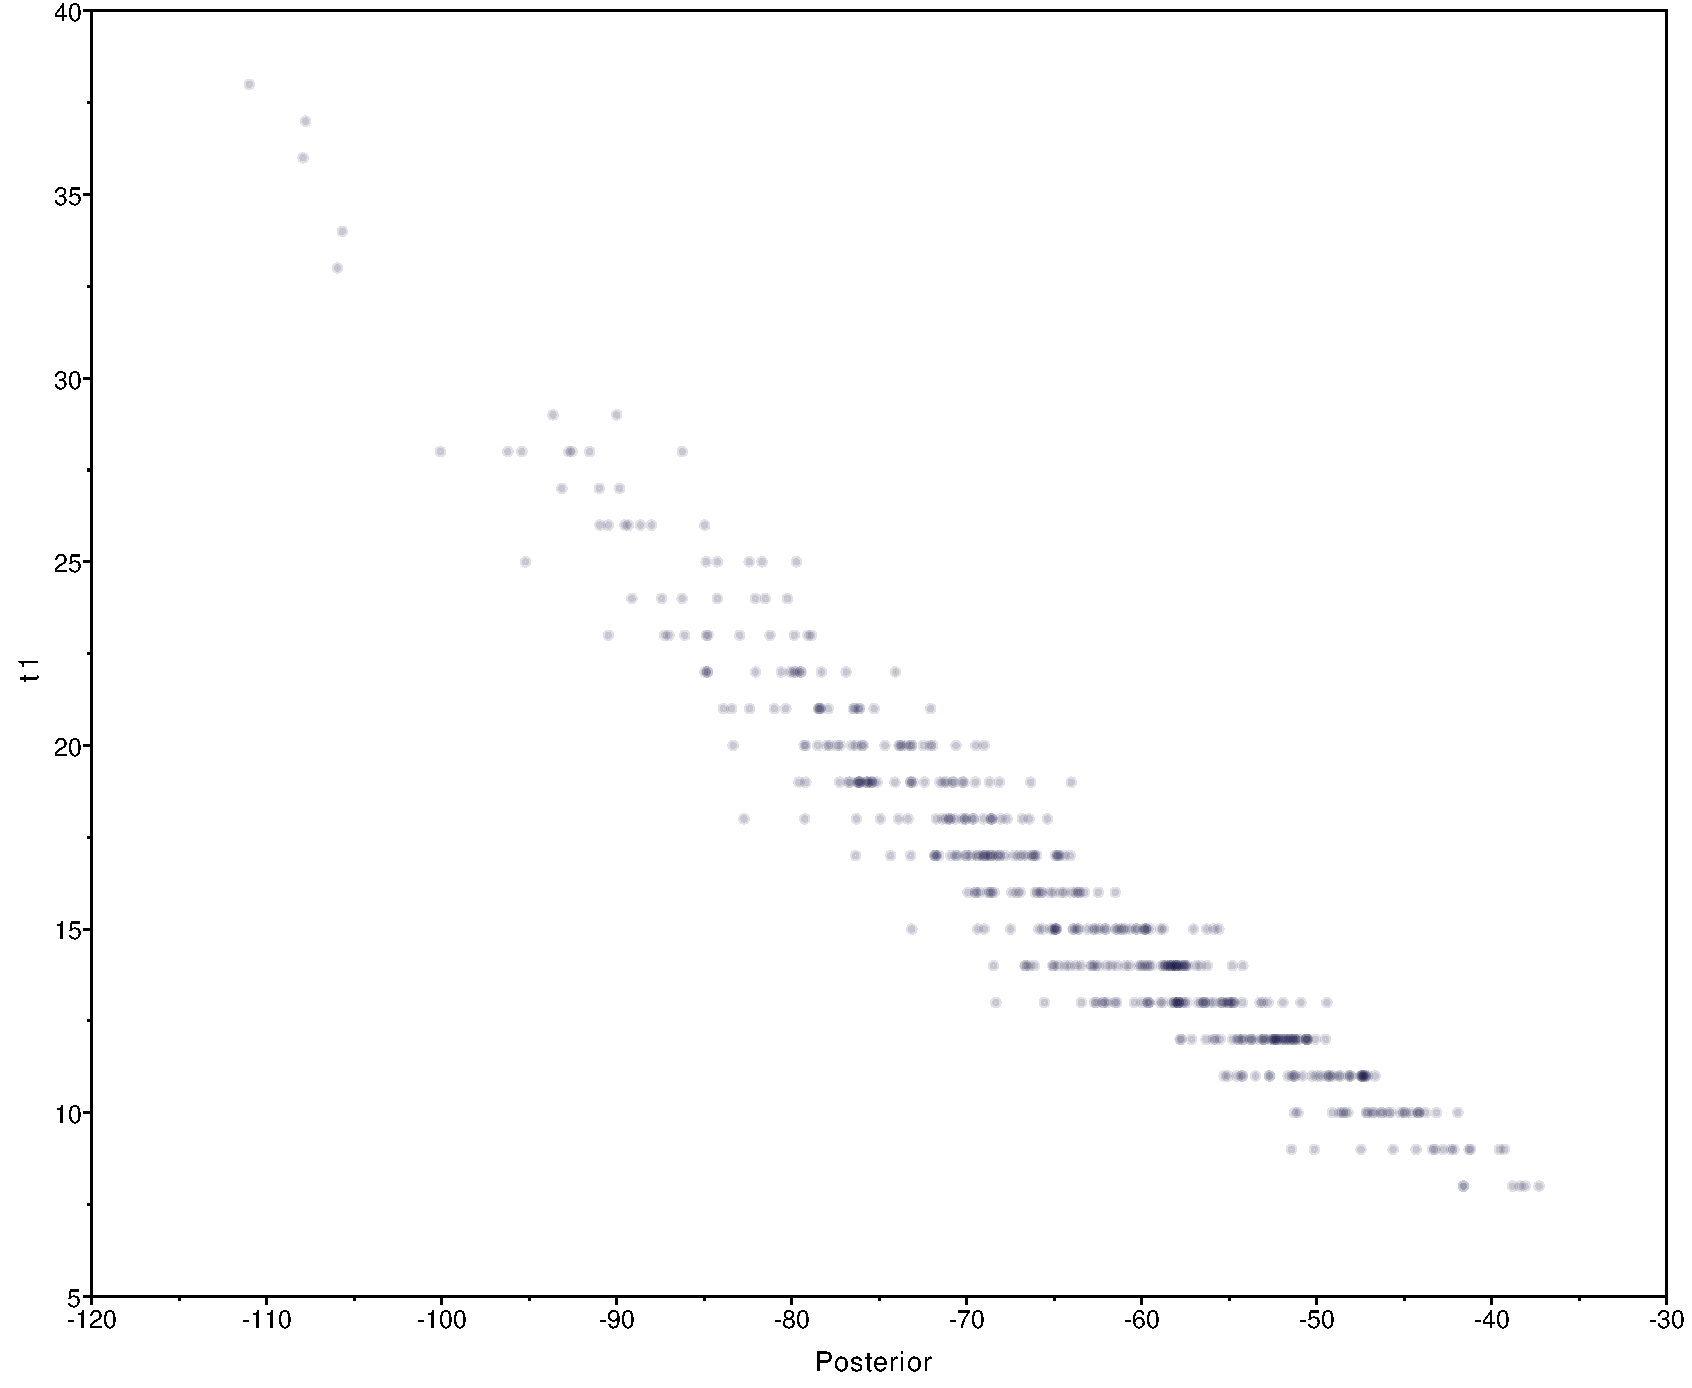
\includegraphics[width=3in]{../RB_Biogeography_Tutorial/figures/joint_ngain_posterior}
\caption{Joint-marginal distribution of posterior and number dispersal events summed over the tree.}
\end{figure}

One interesting facet of this output is there are never fewer than six events.
In fact, since we assume a stratified geography and that only one event may occur per instant, it is impossible to describe the data we see at the tips with fewer than six gain events.
That is, six gain events is part of the maximum parsimony solution.

\subsection{Biogeographic event histories from {\tt mnCharHistoryNewick}}

For more detailed data exploration, this analysis also provides annotated Newick strings with the complete character mappings for the tree.

%\noindent \\ \impmark Open {\tt ./output/bg\_2rate.events.txt} in a text editor.

\begin{framed}
%\begin{lstlisting}[basicstyle=\tiny \listingsfont, columns=texcl]
\begin{lstlisting}
Iteration  Posterior  Likelihood  Prior  Tree
Iteration	Posterior	Likelihood	Prior	Tree
0	-51.3307	-56.0288	4.69806	((((((((P_hawaiiensis_WaikamoiL1[&index=18;nd=0010;pa=0010;ev={}]:0.96 ...
10	-54.4257	-58.1568	3.7311	((((((((P_hawaiiensis_WaikamoiL1[&index=18;nd=0010;pa=0010;ev={}]:0.96 ...
20	-58.0696	-62.0923	4.02274	((((((((P_hawaiiensis_WaikamoiL1[&index=18;nd=0010;pa=0010;ev={}]:0.96 ...
30	-46.5049	-51.1197	4.6148	((((((((P_hawaiiensis_WaikamoiL1[&index=18;nd=0010;pa=0010;ev={}]:0.96 ...
40	-42.8697	-46.4870	3.61735	((((((((P_hawaiiensis_WaikamoiL1[&index=18;nd=0010;pa=0010;ev={}]:0.96 ...
50	-43.5319	-47.4659	3.93394	((((((((P_hawaiiensis_WaikamoiL1[&index=18;nd=0010;pa=0010;ev={}]:0.96 ...

...
\end{lstlisting}
\end{framed}

Each iteration records the data-augmented character history (stochastic mapping) using metadata labels, which, for an internal node, looks like

\begin{snugshade}
\begin{lstlisting}
[&index=23;nd=0110;pa=0010;ch0=0010;ch1=0110;cs=s;bn=16;ev={{t:0.2513,a:1.1195,s:1,i:1}}
\end{lstlisting}
\end{snugshade}

{\tt index=23} indicates this branch leads to the node indexed 23.
The branch began in the ancestral state {\tt pa=0100} and terminated in the state {\tt nd=0110}.
Since this node is not a tip node, it represents a speciation event, so the daughter ranges are also given, {\tt ch0=0010} and {\tt ch1=0110}.
The cladogenic state for this speciation event was subset sympatric, {\tt cs=s}, rather than sympatric (wide or narrow; {\tt w} or  {\tt n}) or allopatric ({\tt a}).
Anagenic dispersal and extinction events occurring along the lineage leading to node 19 are recorded in {\tt events}, where each event has a time (relative to the absolute branch length), absolute age, state (into), and character index ({\tt t}, {\tt a}, {\tt s}, {\tt i}, resp.).
For this posterior sample of the character history for the branch leading to node 22, the species range expanded into Oahu at age 1.1195.

To manipulate this data format, we'll use Python scripts. Below are a few examples of interesting posterior features.

%\noindent \\ \impmark  Open a Python console and read in the events.

\begin{snugshade}
\begin{lstlisting}
> cd scripts
> python27

...

>>> from bg_parse import *
>>> dd=get_events(fn="../output/bg_2rate.events")
\end{lstlisting}
\end{snugshade}

By default, {\tt get\_events()} extracts a dictionary where each node index maps to a branch's character history as reported in {\tt ./input/bg\_2rate.events.txt}. 
Each branch is a dictionary whose keys are various parts of the MCMC state and whose values the MCMC samples.
\begin{snugshade}
\begin{lstlisting}
>>> dd[23].keys()
['ch1', 'iteration', 'bn', 'nd', 'ch0', 'prior', 'posterior', 'cs', 'ev', 'likelihood']
>>> dd[23]['posterior'][0:5]
[-48.6952, -60.1832, -53.2286, -57.5778, -53.4633]
\end{lstlisting}
\end{snugshade}

To get the $n=1$ highest-valued sample for a branch by its posterior value
\begin{snugshade}
\begin{lstlisting}
>>> get_best(dd[23],n=1,p='posterior')
{'prior': [4.48225], 'iteration': [14890], 'bn': [22], 'nd': [[0, 1, 1, 0]], 'ch0': [[0, 1, 1, 0]], 'ch1': [[0, 0, 1, 0]], 'posterior': [-34.7139], 'pa': [[0, 1, 0, 0]], 'cs': ['subset_sympatry'], 'ev': [[{'age': 1.5637, 'state': 1, 'idx': 2, 'time': 0.8611}]], 'likelihood': [-39.1962]}
\end{lstlisting}
\end{snugshade}

To get the probability that area $i$ and area $j$ are both part of the species range as the branch for node 23 terminates, just before the speciation event
\begin{snugshade}
\begin{lstlisting}
>>> get_area_pair(dd[23])
[[0.0816, 0.0188, 0.0628, 0.0000],
 [0.0188, 0.7081, 0.4390, 0.0000],
 [0.0628, 0.4390, 0.7141, 0.0000],
 [0.0000, 0.0000, 0.0000, 0.0000]]
\end{lstlisting}
\end{snugshade}
showing area 3 was occupied nearly with probability 0.71 and both areas 2 and 3 were occupied with probability 0.44.
Note, Hawaii was submerged until approximately 0.5 million years ago, and thus the probability of being in that area is 0.0.

If the range is size one during a speciation event, the cladogenic event state is always narrow sympatric, {\tt `narrow\_sympatry'}.
But given the opportunity for non-sympatric events, i.e. that the range is larger than size one, we can get the probability of cladogenic state using
For the probability for cladogenic event state given the range was larger than size one
\begin{snugshade}
\begin{lstlisting}
>>> get_clado_state(dd[23])
{'allopatry': 0.0224, 'subset_sympatry': 0.1463, 'widespread_sympatry': 0.3183, 'narrow_sympatry': 0.5130}
>>> get_clado_state(dd[23],minSize=2)
{'allopatry': 0.0460, 'subset_sympatry': 0.3005, 'widespread_sympatry': 0.6535, 'narrow_sympatry': 0.0000}
>>> get_clado_state(get_best(dd[23],n=100),minSize=2)
{'allopatry': 0.1290, 'subset_sympatry': 0.6774, 'widespread_sympatry': 0.1936, 'narrow_sympatry': 0.0000}
\end{lstlisting}
\end{snugshade}

Depending on your question, different aspects of the posterior cladogenic state will interest you.
Narrow sympatry is the favored ancestral state, but wide sympatry is favored for ranges of size $n>1$.
However, when we look at the 100 most probable samples, subset sympatry becomes most favored.

More script functions are found in {\tt ./scripts/bg\_parse.py}.

\subsection{New Hampshire extended format file (\texttt{./output/bg\_2rate.nhx})}

Because this data is very high-dimensional, we'll use an external data exploration tool to look at range evolution.

This file summarizes the input and output from a BayArea analysis using NEXUS format containing a New Hampshire eXtended (NHX) tree string.
NHX allows you to annotate nodes in a Newick string with meta-information, which BayArea uses to report the probabilities in the \texttt{my\_run.area\_probs.txt} file.
The \texttt{geo} block gives the geographical latitudes and longitudes for the areas in the order they are reported as probabilities.
Like the \texttt{my\_run.area\_probs.txt} file, this file is not written until the analysis is complete.
This annotation is used for the two visualization programs covered in the next section, Phylowood and BayArea-Fig.
The anatomy of the Phylowood and BayArea-Fig settings blocks will also be explained there.

\section{Visualization}

Here we'll explore two options for visualizing ancestral range reconstructions.
I'll walk you through some of the basic functionality, but feel free to play around as you like.

\subsection{Phylowood}

Phylowood generates interactive animations to explore biogeographic reconstructions.

%\noindent \\ \impmark Open \texttt{http://mlandis.github.io/phylowood}.

%\noindent \\ \impmark Drag and drop \texttt{./output/bg\_2rate.nhx.txt} into the text field.

\begin{figure}[H]
\centering
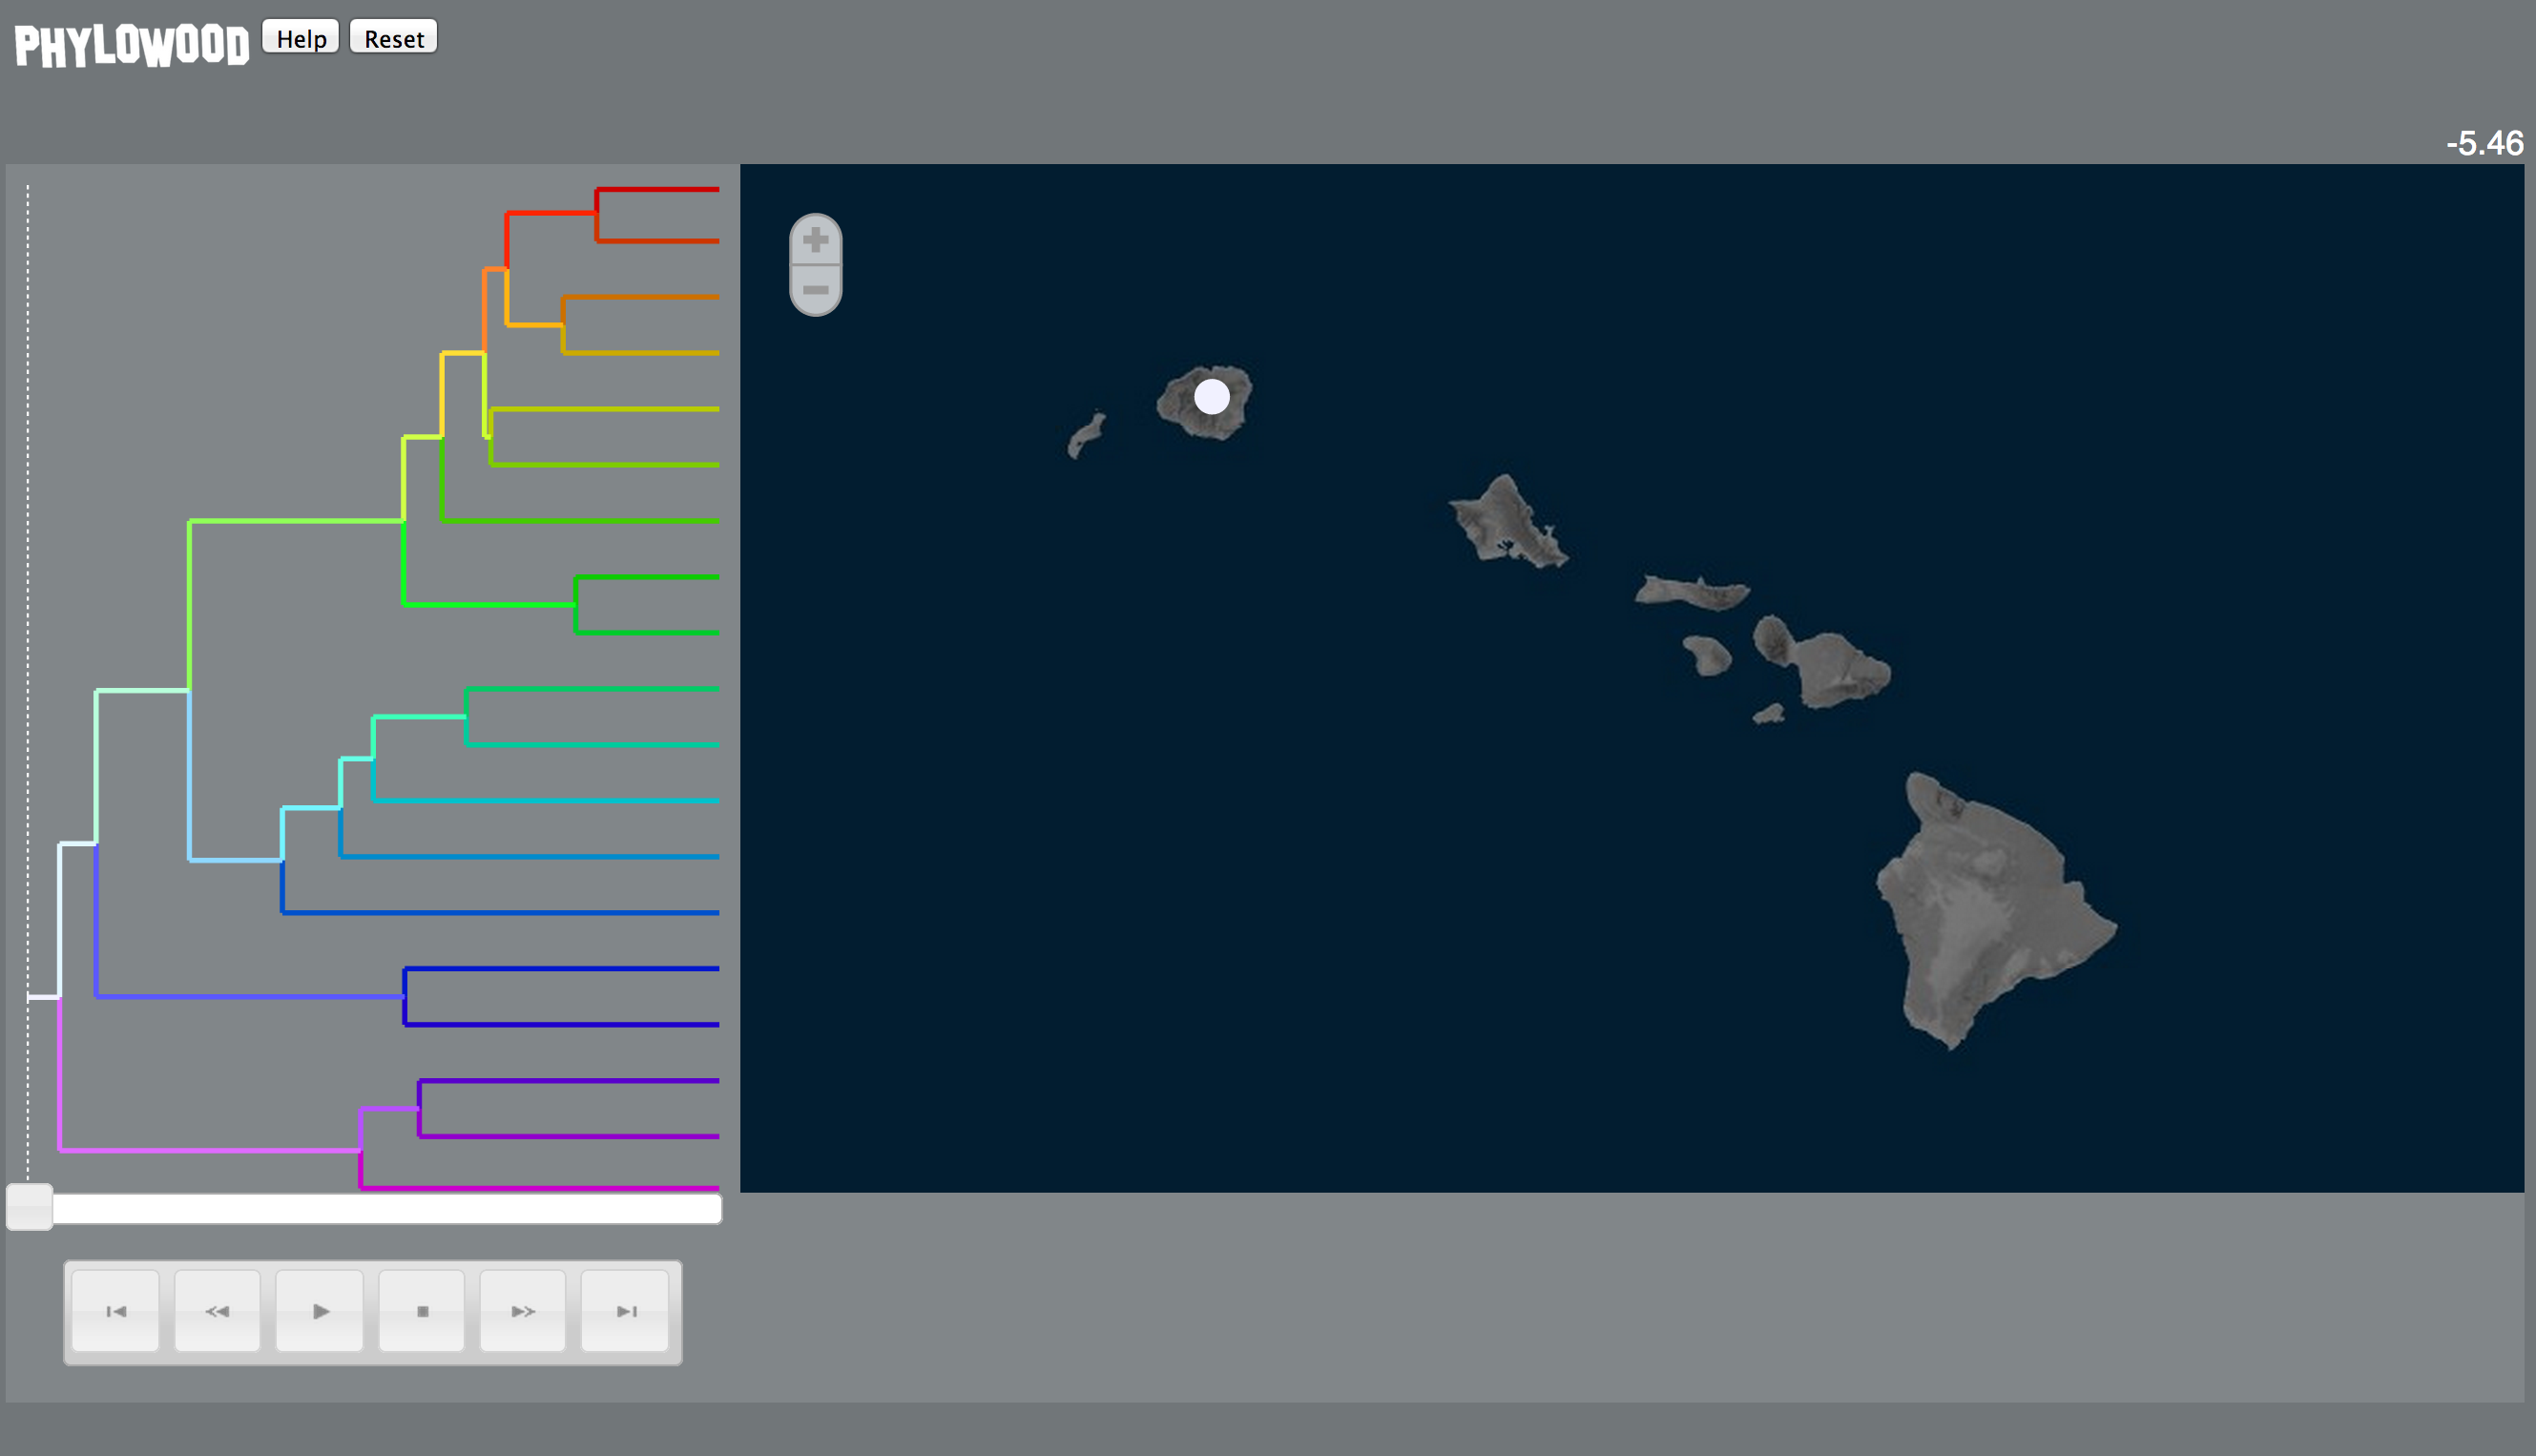
\includegraphics[width=4in]{../RB_Biogeography_Tutorial/figures/phw_mrca}
\caption{Phylowood frame showing posterior ancestral range of root node.}
\end{figure}

%\noindent \\ \impmark Click the Play button to view the animation. \\

There are three control panels to help you filter data: the media panel, the map panel, and the phylogeny panel.
The media buttons correspond to Beginning, Slow/Rewind, Play, Stop, Fast Forward, Ending (from left to right).
The animation will play the timeframe corresponding to the slider.

%\noindent \\ \impmark Drag the slider to the right (the present).

\begin{figure}[H]
\centering
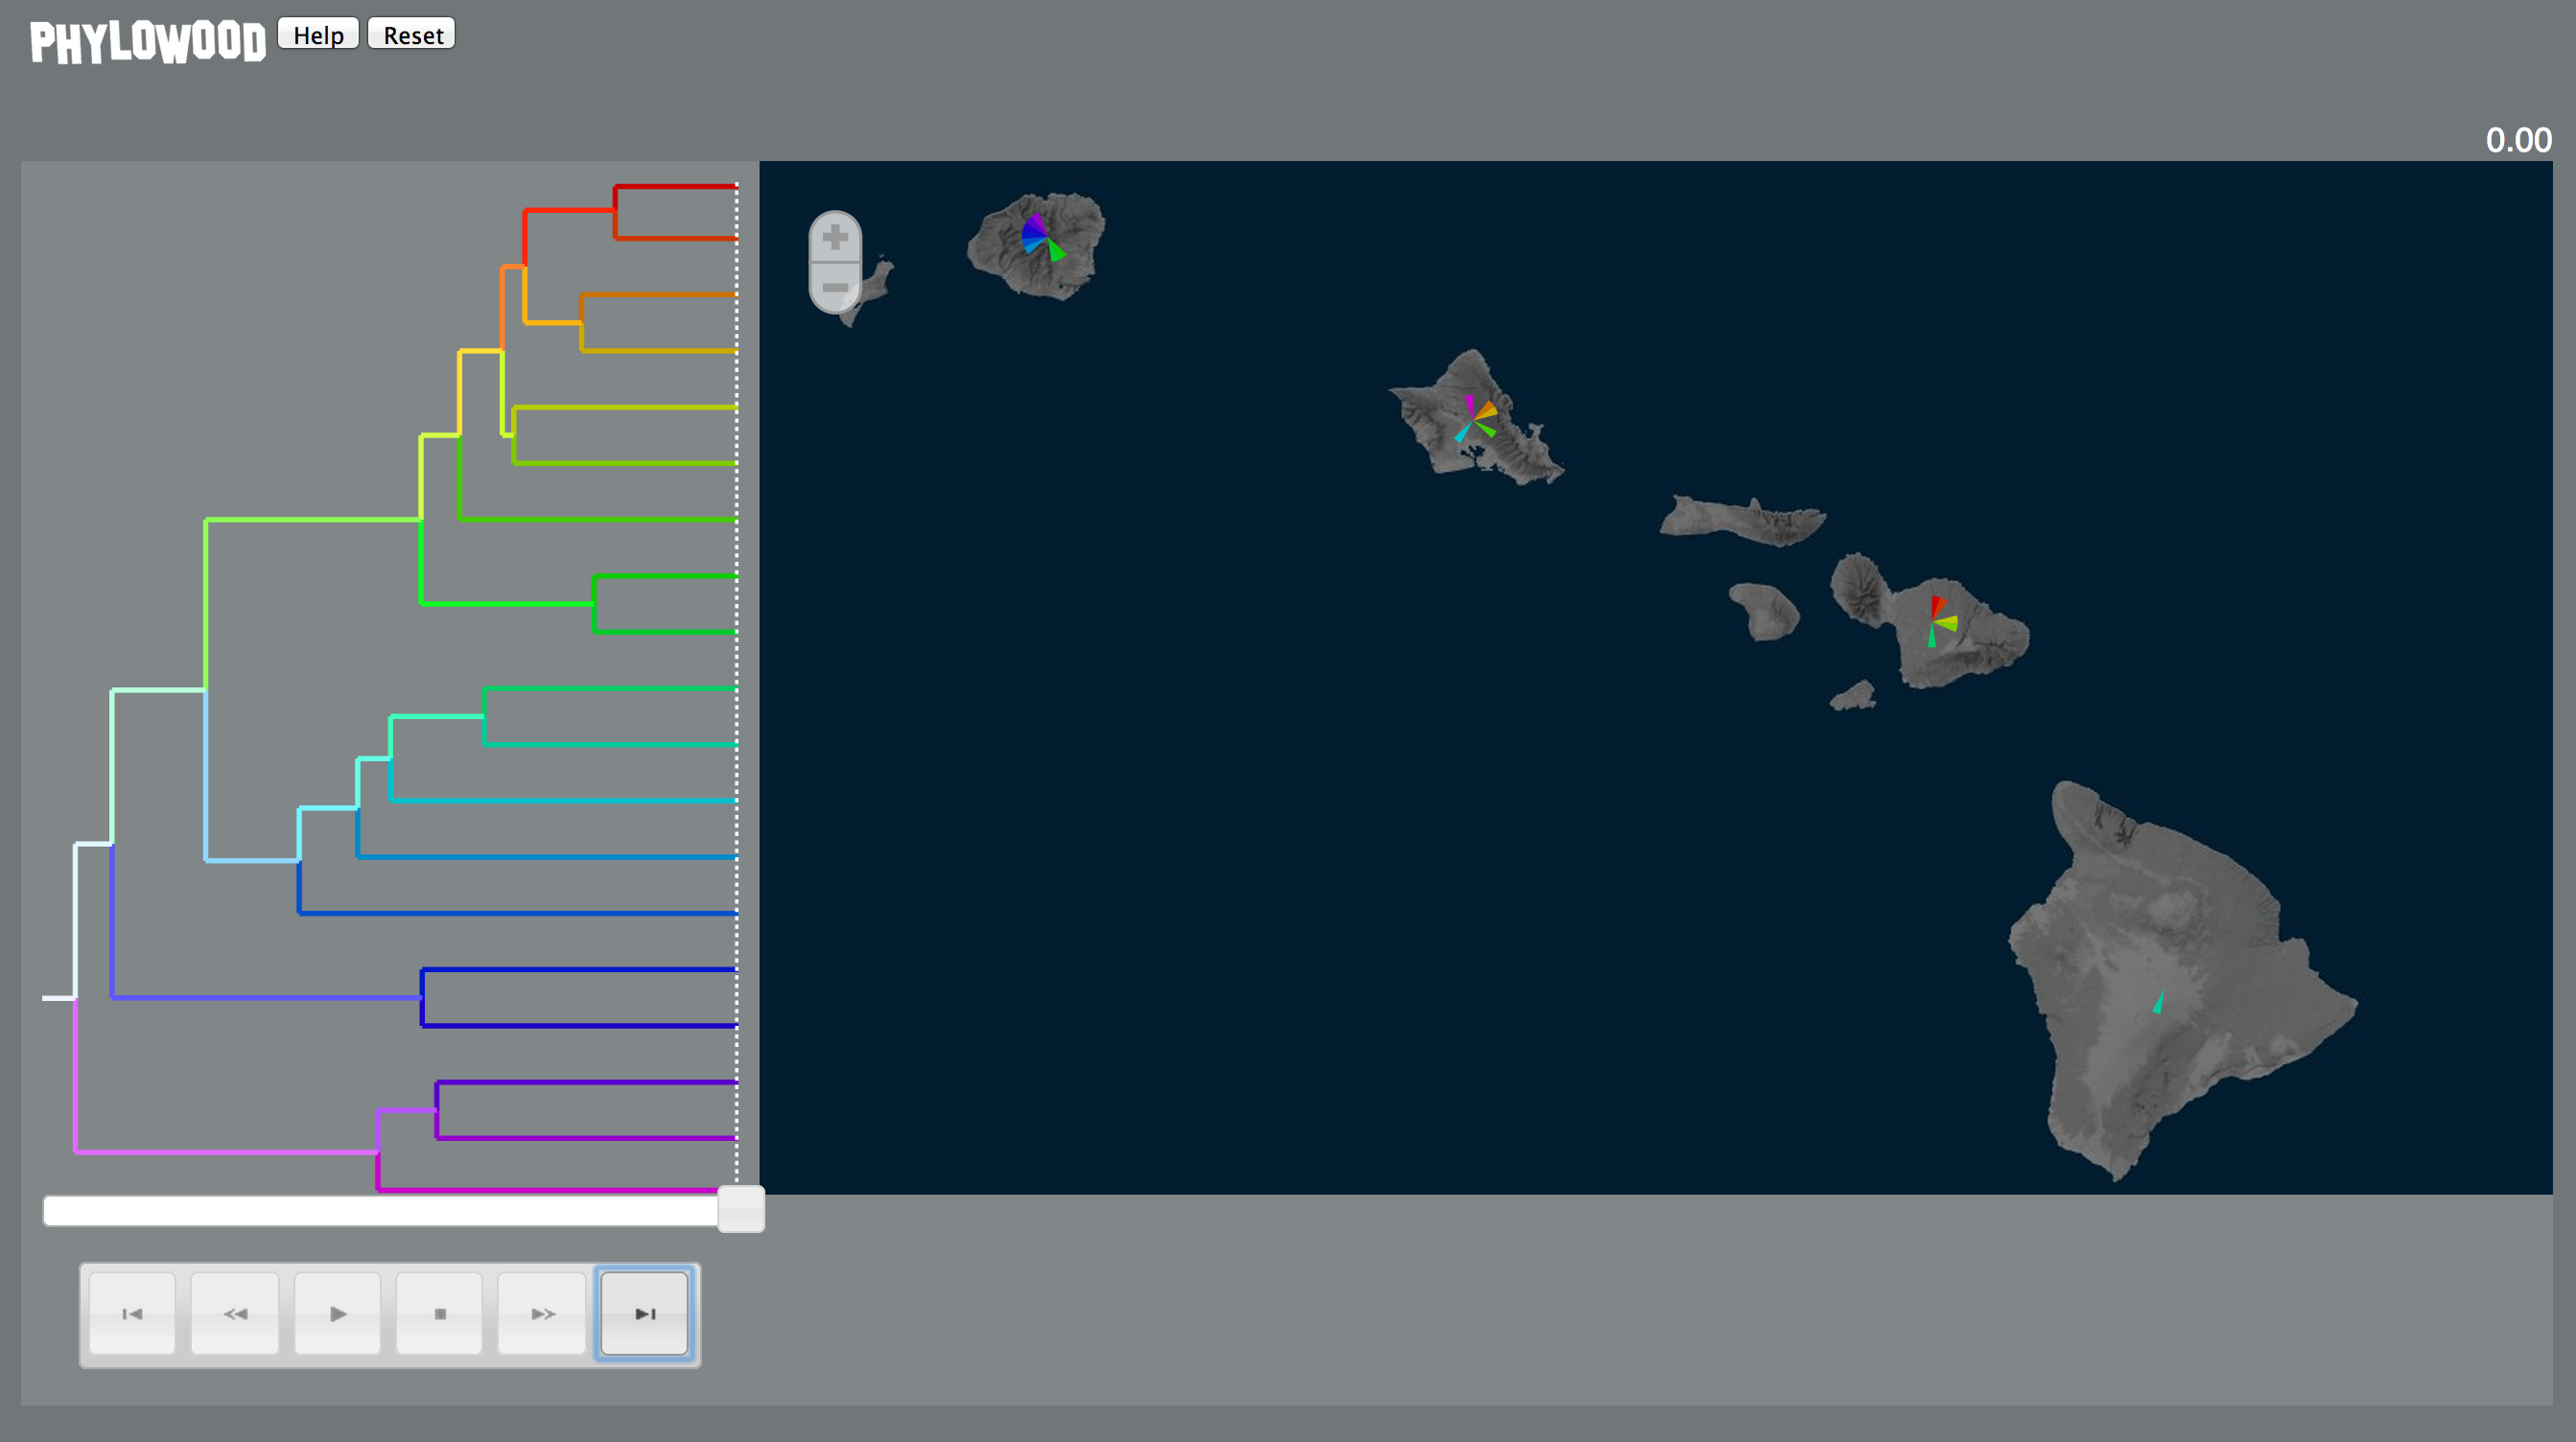
\includegraphics[width=4in]{../RB_Biogeography_Tutorial/figures/phw_all}
\caption{Phylowood frame showing distribution of extant taxon ranges.}
\end{figure}

%\noindent \\ \impmark Pan and zoom around the map.\\

Marker colors correspond to the phylogenetic lineages in the phylogeny panel.
Markers are split into slices and (loosely) sorted phylogenetically, so nearby slices are generally closely related.
At divergence events, a marker's radius is proportional to the marginal posterior probability the node was present in the area at that time.
Between divergence events, marker's radius is simply an interpolation of the values at the two endpoints.
Some information about geological constraints and cladogenic events is lost.

%\noindent \\ \impmark Mouseover an area to learn which lineage it belongs to and its presence probability. \\

Since it's difficult to see how specific clades evolve with so many taxa, Phylowood offers two ways to filter taxa from the animation.
We call the set of a lineage, all its ancestral lineages towards the root, and all descendant lineages a phylogenetic heritage.
The root's heritage is the entire clade.
A leaf node's heritage is a path from the tip to the root.

%\noindent \\ \impmark Mouseover a lineage to temporarily highlight the lineage's heritage. Remove the mouseover to remove the highlight effect. \\

The highlight effect is temporary and quickly allows you to single out lineages of interest during animation.
Phylowood also offers a masking effect that persists until an unmask command is issued.

%\noindent \\ \impmark Double-click the white root branch to mask the root node's heritage (all lineages). Single click a lineage to unmask that lineage's heritage. \\

\begin{figure}[H]
\centering
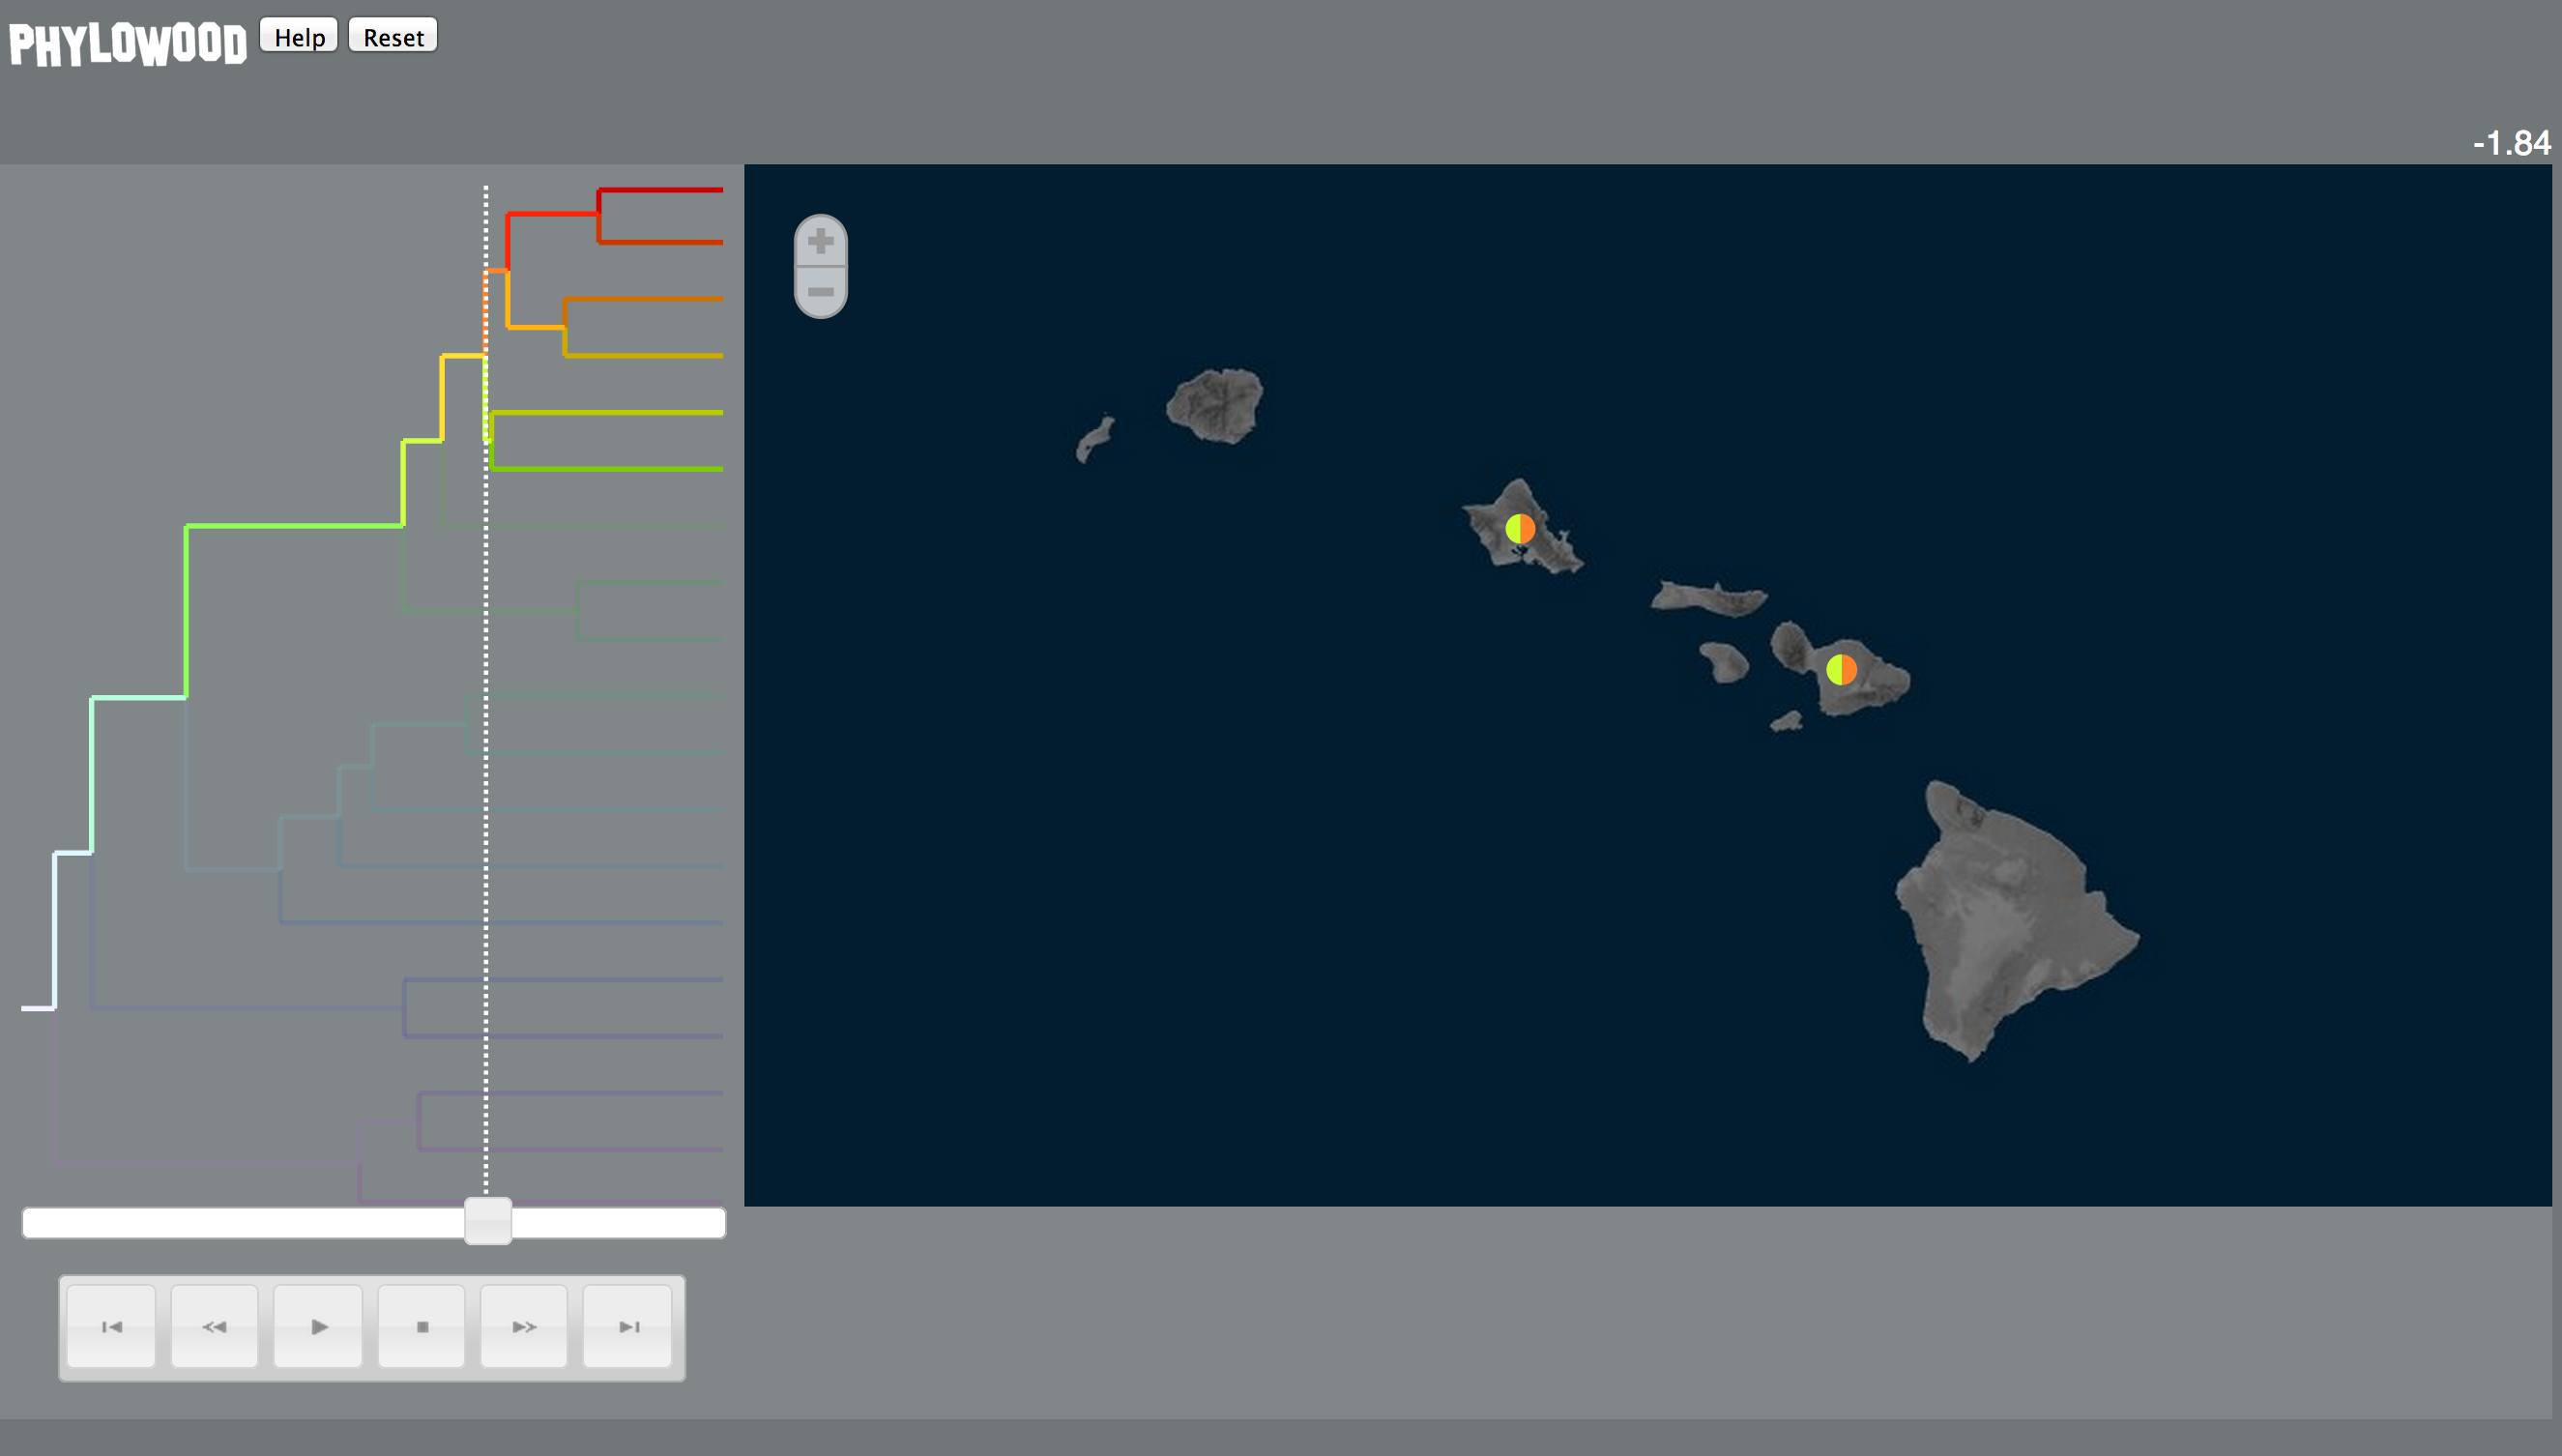
\includegraphics[width=4in]{../RB_Biogeography_Tutorial/figures/phw_br23}
\caption{Phylowood frame highlighting the posterior range for the most recent common ancestor of {\it P. mauiensis} and {\it P. hawaiiensis}.}
\end{figure}

Now that the masking effects are in place, you're free to interact with other map components.
In addition, the area of marker sizes is only distributed among unmasked lineages.

%\noindent \\ \impmark Visit \texttt{https://github.com/mlandis/phylowood/wiki} to learn more about Phylowood.

%\bibliography{bayes}




\newrefsection
\chapter{Phylogenetic Comparative Analyses: Continuous Trait Evolution}
\section{Introduction}

The subject of the comparative method is the analysis of trait evolution at the macroevolutionary scale.
In a comparative context, many different questions can be addressed: tempo and mode of evolution, correlated evolution of multiple quantitative traits, trends and bursts, changes in evolutionary mode correlated with major key innovations in some groups, etc \citep[see][for a good introduction]{Harvey:1991p899}.

In order to correctly formalize comparative questions, the underlying phylogeny should always be explicitly accounted for. This point is clearly illustrated, in particular, by the independent contrast method \citep{Felsenstein:1985p686}. Practically speaking, the phylogeny and the divergence times are usually first estimated using a separate phylogenetic reconstruction software. In a second step, this time-calibrated phylogeny is used as an input to the comparative method.
Doing this, however, raises a certain number of methodological problems:
\begin{itemize}
\item
the uncertainty about the phylogeny (and about divergence times) is ignored
\item
the traits themselves may have something to say about the phylogeny
\item
the rate of substitution, and more generally the parameters of the substitution process, can also be seen as quantitative traits, amenable to a comparative analysis.
\end{itemize}
All these points are not easily formalized in the context of the step-wise approach mentioned above.
Instead, what all this suggests is that phylogenetic reconstruction, molecular dating and the comparative method should all be considered jointly, in the context of one single overarching probabilistic model.

Thanks to its modular structure, RevBayes represents a natural framework for attempting this integration.
The aim of the present tutorial is to guide you through a series of examples where this integration is achieved, step by step.
It can also be considered as an example of the more general perspective of \emph{integrative modeling}, which can be recruited in many other contexts.

\section{Data and files}

In the \cl{data} folder, you will find the following files
\begin{itemize}
\item
\cl{plac40lhtlog.nex}: 3 life-history traits (age at sexual maturity, body mass, maximum recorded lifespan) for 40 placental mammals \citep[taken from the Anage database,][]{deMagalhaes:2009p991}. The traits have been log-transformed.
\item
\cl{plac40\_4fold.nex}: an alignment made of a concatenation of 17 nuclear genes in 40 placental mammals \citep[from][]{Lartillot:2012be}, with only the four-fold degenerate third coding positions.
\item
\cl{chronoplac40.tree}: a time-calibrated phylogeny, which has been obtained by running another software program \citep[PhyloBayes,][]{Lartillot:2009p884}.
On the cluster, and if you are logged under an X-terminal, you can visualize this tree using the \cl{njplot} command:
\\
\cl{njplot chronoplac40.tree}
\item
\cl{archaeaRNA.nex}: an alignment of rRNA sequences of 33 archaeal species.
\item
\cl{archaeaTemp.nex}: optimal growth temperatures for the 33 archaeal species.
\end{itemize}

\section{Univariate Brownian evolution of quantitative traits}

\label{univariate}

As a first preliminary exercise, we wish to reconstruct the evolution of body mass in placental mammals and, in particular, estimate the body mass of their last common ancestor.
For this, we will assume that the logarithm of body mass follows a simple univariate Brownian motion along the phylogeny.
In a first step, we will ignore phylogenetic uncertainty:
thus, we will assume that the Brownian process describing body mass evolution runs along a fixed time-calibrated phylogeny (with fixed divergence times), such as specified in the file \cl{chronoplac40.tree}.

You may want to take the time to visualize the tree given in \cl{chronoplac40.tree} as well as the matrix of quantitative traits specified by the \cl{plac40lhtlog.nex} file, before going into the modeling work described below.

\subsection{The model and the priors}

A univariate Brownian motion $x(t)$ is parameterized by its starting value at the root of the phylogeny $x(0)$ and a rate parameter $\sigma$. This rate parameter tunes the amplitude of the variation per unit of time. Specifically, along a given time interval $(0,T)$, the value of $X$ at time $T$ is normally distributed, with mean $x(0)$ and variance $\sigma^2 T$:
\begin{eqnarray*}
x(T) &\sim& \text{Normal} \left( x(0), \sigma^2 T \right).
\end{eqnarray*}

Concerning $\sigma$, we can formalize the idea that we are ignorant about the \emph{scale} (the order of magnitude) of this parameter by using a log-uniform prior:
\begin{eqnarray*}
\sigma &\sim& \frac{1}{\sigma}.
\end{eqnarray*}

Concerning the initial value $x(0)$ of the Brownian process at the root of the phylogeny,
the current version of RevBayes only implements a uniform prior.
This is done by default (no need to explicitly define it).

Finally, the tree topology $\psi$ is, as mentioned above, fixed to some externally given phylogeny.
The entire model is now specified: tree $\psi$, variance $\sigma$ and Brownian process $x(t)$:
\begin{eqnarray*}
\sigma &\sim& \frac{1}{\sigma},
\\
x(0) &\sim& \text{Uniform},
\\
x(t) \mid \Psi, \sigma &\sim& \text{Brownian} \left( x(0), \, \psi, \, \sigma \right).
\end{eqnarray*}
Conditioning the model on empirical data by clamping $x(t)$ at the tips of the phylogeny, we can then run a MCMC to sample from the joint posterior distribution on $\sigma$ and $x$. Once this is done, we can obtain posterior means, medians or credible intervals for the value of body mass or other life-history traits for specific ancestors.


\subsection{Programming the model in RevBayes}

In \cl{tutorials/NESCent/RevBayes\_scripts/}, you will find a script called \cl{placentaliaMass.Rev}.
This script implements the univariate Brownian model described above. Instead of re-typing the content of script entirely in the context of an interactive \cl{RevBayes} session, you can instead run the script directly, by first going to the \cl{tutorials/NESCent/} folder and then giving the script as an argument to the \cl{RevBayes} program:
\\
\cl{RevBayes RevBayes\_scripts/placentaliaMass.Rev}.

This script essentially reformulates what has been explained in the last subsection, now in the Rev language:
\begin{itemize}
\item
load trait data:
\\
\cl{contData <- readCharacterData("data/plac40lhtlog.nex")}
\item
load the time-tree from file:
\\
\cl{treeArray <- readTrees("data/chronoplac40.tree"
\\
psi <- treeArray[1]
}
\item
define $\sigma$, with a truncated log-uniform prior:
\\
\cl{sigma $\sim$ \text{dnLogUniform}(min=0.001,max=1000)}
\\
to accelerate convergence, it can be useful to force initialization of $\sigma$ to a small value:
\\
\cl{sigma.setValue(0.1)}
\item
define the multivariate Brownian process, which we will call \cl{logmass}:
\\
\cl{logmass $\sim$ dnBrownian(psi,sigma)}
\item
condition the Brownian model on empirically observed values for body mass in extant taxa.
Here, we need to specify that body mass is the second column of the dataset:
\\
\cl{
logmass.clampAt(contData,2)
}
\end{itemize}
The model is now entirely specified. We can define the moves on its parameters:
\begin{itemize}
\item
initialize a running index for storing moves:
\\
\cl{index <- 1}
\item
push a scaling move on $\sigma$:
\\
\cl{
moves[index] <- mvScale(sigma, lambda=2.0, tune=true, weight=3.0)
\\
index <- index + 1
}
\item
a sliding move on the Brownian process
\\
\cl{
moves[index] <- mvRealNodeValTreeSliding(process=logmass, lambda=10, tune=true, weight=100)
\\
index <- index + 1
}
\item
a global translation move on the Brownian process:
\\
\cl{
moves[index] <- mvRealNodeValTreeTranslation(process=logmass,lambda=1,
\\
tune=true,weight=1)
\\
index <- index + 1
}
\item
before creating the model, we define summary statistics, to be monitored during the MCMC: the mean and the standard deviation of the trait across the tree:
\\
\cl{
meanlogmass := logmass.mean()
\\
stdevlogmass := logmass.stdev()
}
\item
as well as the value of the log of body mass for the root:
\\
\cl{
rootlogmass := logmass.rootVal()
}
\item
now, create the model
\\
\cl{
mymodel <- model(sigma)
}
\item
make a screen monitor that tracks the summary statistics of interest:
\\
\cl{
monitors[1] <- mnScreen(printgen=10, sigma, rootlogmass, meanlogmass, stdevlogmass)
}
\item
a file monitor that does the same thing, but directly into a file:
\\
\cl{
monitors[2] <- mnFile(filename="output/placmass.trace", printgen=10, separator = "       ", sigma, rootlogmass, meanlogmass, stdevlogmass)
}
\item
a file monitor for the ancestral reconstruction of traits along the entire tree (in newick format):
\\
\cl{
monitors[3] <- mnFile(filename="output/placmass.logmass", printgen=10, separator = "       ", logmass)
}
\item
and a general model monitor:
\\
\cl{
monitors[4] <- mnModel(filename="output/placmass.log", printgen=10, separator = " ")
}
\end{itemize}
We can finally create a mcmc, and run it for a good 100 000 cycles:
\\
\cl{
mymcmc <- mcmc(mymodel, monitors, moves)
\\
mymcmc.burnin(generations=100,tuningInterval=100)
\\
mymcmc.run(100000)
}

\subsection*{Exercises}

\begin{itemize}
\item
run the model, check convergence and obtain a sample from the posterior distribution
\item
using \cl{Tracer}, visualize the posterior distribution on ancestral placental body mass
\item
calculate the 95\% credible interval for ancestral body mass
\item
calculate the 95\% credible interval for the rate of evolution of the log of body mass ($\sigma$)
\end{itemize}



\section{Correlated evolution of multiple traits}
\label{multivariate}

Next, we would like to estimate the correlation between the $K=3$ life-history traits given in the \cl{plac40lhtlog.nex} file, while properly taking into account phylogenetic inertia. 
To do so, we will assume that the traits jointly evolve along the phylogeny as a \emph{multivariate} Brownian process.
We will estimate the \emph{covariance matrix} of this process and assess the empirical support in favor of positive or negative correlations between pairs of traits in terms of posterior probabilities of having positive or negative entries in this covariance matrix.
At this stage of the tutorial, we will again ignore phylogenetic uncertainty.

\subsection{The model and the priors}

A multivariate Brownian process $X(t)$, of dimension $K$ (here $K=3$),
is entirely parameterized by its starting value ($X(0)$ at the root of the phylogeny, which a vector of dimension $K$) and a $K \times K$ symmetric positive matrix (the covariance matrix), which we will call $\Sigma$.
A positive entry between two traits, say $\Sigma_{12} > 0$, means that when trait 1 increases, trait 2 also tends to increase. Conversely, a negative entry means that the two traits tend to undergo variation in opposite directions.
As for the diagonal entries (e.g. $\Sigma_{11}$), they represent the variance per unit of time (i.e. the rate of evolution) of each trait considered marginally,
thus very much like $\sigma^2$ (\emph{not} $\sigma$) in the univariate model of the previous section.

On $\Sigma$, we will assume an inverse-Wishart prior:
\begin{eqnarray*}
\Sigma &\sim& W^{-1}(\Sigma_0, d),
\end{eqnarray*}
where $\Sigma_0$ is a multiple of the identity matrix (i.e. $\Sigma_0 = \kappa I_K$), for some positive real number $\kappa$.
Using a prior centered on a diagonal matrix means that we want to be indifferent with respect to either positive or negative correlations among traits. As for the parameter $\kappa$, it will set the amplitude of the variation per unit of time of the traits. Since we have no idea about the scale of this parameter, we can use a log-uniform prior:
\begin{eqnarray*}
\kappa &\sim& \frac{1}{\kappa}.
\end{eqnarray*}
This completes our model:
\begin{eqnarray*}
\kappa &\sim& \frac{1}{\kappa},
\\
\Sigma \mid \kappa &\sim& W^{-1}(\Sigma_0 = \kappa I_K , \, d = K+2),
\\
X(0) &\sim& \text{Uniform},
\\
X(t) \mid X(0), \Psi, \Sigma &\sim& \text{Brownian}(X(0), \, \psi, \, \Sigma).
\end{eqnarray*}
As in the univariate case, we can then clamp $X$ at the tips of the phylogeny and sample from the joint distribution over the parameters of the model by MCMC.
Once this is done, we can estimate marginal posterior probabilities (e.g. for positive or negative covariance among traits) and infer ancestral traits.

\subsection*{Programming the model in RevBayes}

You may find it convenient to program this multivariate model by first duplicating the script of the univariate model:
\\
\cl{cp placentaliaMass.Rev placentaliaTraits.Rev}
\\
Then, you can edit the new script, \cl{placentaliaTraits.Rev}, and introduce the modifications that would change the univariate model
into its multivariate counterpart.

In the following, only those aspects of the multivariate model that differ from the univariate case are outlined.
Essentially, instead of a univariate Brownian motion parameterized by a scalar parameter, you now need to:
\begin{itemize}
\item
define $\kappa$:
\\
\cl{kappa $\sim$ \text{dnLogUniform}(min=0.001,max=1000)}
\item
define the number of degrees of freedom as $d = K+2$:
\\
\cl{df <- nTraits+2}
\item
define the covariance matrix $\Sigma$ as inverse Wishart:
\\
\cl{Sigma $\sim$ dnInvWishart(dim=nTraits, kappa=kappa, df=df)}
\item
define the multivariate Brownian process:
\\
\cl{X $\sim$ dnBrownianMultiVariate(psi,Sigma)}
\item
condition the Brownian model on quantitative trait data.
This needs to be done separately for each trait:
\\
\cl{
for (i in 1:nTraits)    \{
        X.clampAt(contData,i,i)
\}
}
\\
Here, we give twice the index \cl{i} to the \cl{clampAt} function: the first corresponds to the entry of the Brownian process, and the second one to the column of the data matrix. In some cases (as we will see below), the Brownian process and the data matrix may not be of same dimension, and therefore, it will be useful to be able to specify arbitrary maps between them.
\end{itemize}
The model is now entirely specified. We can define the moves on its parameters.
\begin{itemize}
\item
initialize a running index for storing moves:
\\
\cl{index <- 1}
\item
push a scaling move on $\kappa$:
\\
\cl{
moves[index] <- mvScale(kappa, lambda=2.0, tune=true, weight=3.0)
\\
index <- index + 1
}
\item
a sliding move on the Brownian process
\\
\cl{
moves[index] <- mvMultivariateRealNodeValTreeSliding(process=X, lambda=10,
\\
tune=true,weight=100)
\\
index <- index + 1
}
\item
a global translation move on the Brownian process (component-wise, that is, a random global translation across the entire phylogeny is applied to one trait taken at random):
\\
\cl{
moves[index] <- mvMultivariateRealNodeValTreeTranslation(process=X, lambda=1,
\\
tune=true, weight=1)
\\
index <- index + 1
}
\item
finally, a conjugate Gibbs move for $\Sigma$: as it turns out, conditional on $\kappa$ and the Brownian process $X$, it is possible to directly resample $\Sigma$ from its conditional posterior distribution \citep{Lartillot:2011p55}. In RevBayes, this is implemented as follows:
\\
\cl{
moves[index] <- mvConjugateInverseWishartBrownian(sigma=Sigma, process=X,
\\
kappa=kappa, df=df, weight=1)
\\
index <- index + 1
}
\end{itemize}
Before creating the model, we need to define a few summary statistics, which we want to track during MCMC, either to monitor convergence or for obtaining interesting outputs.
First, suppose you are specifically interested in the covariance and the correlation coefficient associated with the joint variation of body-size (trait 2) and longevity (trait 3). You may also be interested in the \emph{partial} correlation coefficient between body mass and longevity, i.e. while controlling for variation in age at sexual maturity. These three quantities can be singled out and named as follows:
\begin{itemize}
\item
the covariance:
\\
\cl{
cov23 := Sigma.covariance(2,3)
}
\item
the correlation coefficient:
\\
\cl{
cor23 := Sigma.correlation(2,3)
}
\item
the variance per unit of time of, say, log body mass, which is given by the diagonal entry:
\\
\cl{
var2 := Sigma.covariance(2,2)
}
\item
we can also get all correlation coefficients into a single vector (you can skip this part during the session and leave it as  homework):
\begin{verbatim}
# initialize a running index
corrindex <- 1
# loop over all pairs of traits
for (i in 1:(nTraits-1))    {
    for (j in (i+1):nTraits) {
        correl[corrindex] := Sigma.correlation(i,j)
        corrindex <- corrindex + 1
    }
}
\end{verbatim}
\item
we could be interested in tracking several summary statistics also for the Brownian motion, in particular the mean along the tree, separately for each trait:
\begin{verbatim}
for (i in 1:nTraits)    {
        meanX[i] := X.mean(i)
}
\end{verbatim}
\end{itemize}
After creating the model, all these new variables (\cl{cor12}, \cl{correl}, \cl{meanX}, etc) can be monitored, along with the other parameters of the model:
\begin{itemize}
\item
create the model
\\
\cl{
mymodel <- model(kappa)
}
\item
make a screen monitor that tracks correlation coefficients and mean Brownian values:
\\
\cl{
monitors[1] <- mnScreen(printgen=10, correl, meanX)
}
\item
a file monitor that does the same thing, but directly into a file:
\\
\cl{
monitors[2] <- mnFile(filename="output/plactraits.trace", printgen=10, separator = "       ", correl, meanX)
}
\item
a file monitor for $\Sigma$:
\\
\cl{
monitors[3] <- mnFile(filename="output/plactraits.cov", printgen=10, separator = "  ", Sigma)
}
\item
a file monitor for the ancestral reconstruction of traits:
\\
\cl{
monitors[4] <- mnFile(filename="output/plactraits.traits", printgen=10, separator = "       ", X)
}
\item
and a general model monitor:
\\
\cl{
monitors[5] <- mnModel(filename="output/plactraits.log", printgen=10, separator = " ")
}
\end{itemize}
We can finally create the mcmc and run it:
\\
\cl{
mymcmc <- mcmc(mymodel, monitors, moves)
\\
mymcmc.burnin(generations=100,tuningInterval=100)
\\
mymcmc.run(100000)
}

\subsection*{Exercises}

\begin{itemize}
\item
using \cl{Tracer}, visualize the posterior distribution on the correlation coefficient between mass and longevity.
\item
estimate the posterior mean, median and 95\% credible interval for this correlation coefficient.
\item
does the credible inrerval overlap 0? What does that say about the empirical support for the correlation between body mass and longevity?
\item
what proportion of the variation in longevity among placental mammals is explained by body mass?
\end{itemize}


\section{Accounting for uncertainty in divergence times}

Starting from the model implemented in the last section, we now want to account for phylogenetic uncertainty. As first pointed out by \cite{Huelsenbeck:2003p999}, this can easily be done in a Bayesian framework, through the use of a joint model combining sequence data and quantitative traits. Specifically:
\begin{itemize}
\item
two data sets are loaded: one for sequence data and one for quantitative traits
\item
a tree is defined (here, with a uniform prior, but this could be a birth death or anything else)
\item
a Brownian model is defined over the tree (just as described in the previous section)
\item
the Brownian model is conditioned on the quantitative trait data
\item
a substitution model is defined over the same tree
\item
the substitution model is conditioned on the molecular sequence data.
\end{itemize}
Instead of remaining fixed to a pre-defined value,
the tree should now be moved during the MCMC.
%If the sequence data are sufficiently informative, they will induce a relatively well-focussed posterior distribution
%over the tree.
%The uncertainty about correlation parameters
%will then be automatically integrated over this posterior distribution.
Ideally, we would like to move both the toplogy and the divergence times.
Mixing over tree topologies under a Brownian model is relatively challenging, however
(it works, but it requires rather long MCMC runs).
For that reason, in the following, we will mix over divergence times only,
under the constraint of a fixed tree topology.
The features of the model that would need to be modified in order to also mix over topologies
will nevertheless be indicated. You may want try them after the workshop.

\subsection{Programming the model in RevBayes}

Implementing this joint model in RevBayes is just a matter of
adding the following features to the model defined in the previous section
(after duplicating the script):
\begin{itemize}
\item
instead of having a fixed tree, we should now define a \cl{random} tree. We could use a birth death prior, whose speciation and extinction rates are themselves endowed with some diffuse exponential prior:
\\
\cl{
speciation $\sim$ dnExp(0.1)
\\
extinction $\sim$ dnExp(0.1)
\\
sampling\_fraction := 0.01  \, \, \,    \# 40 out of the $\sim$4000 placental mammals
\\
psi $\sim$ dnBDP(lambda=speciation, mu=extinction, rho=sampling\_fraction, rootAge=1.0, nTaxa=nTaxa, names=names)
}
\item
we still want to work on a fixed, pre-specified, tree topology (thus, the birth-death prior will be used here only for averaging over uncertainty about divergence times):
\\
\cl{
treeArray <- readTrees("data/chronoplac40.tree")
\\
fixedTree <- treeArray[1]
\\
psi.setValue(fixedTree)
}
\item
create a substitution model, just like what you probably did in previous sessions. In a first step, you can use a simple GTR model, without any rate variation, neither among sites nor among branches.
\item
load the sequence data matrix specified in \cl{data/plac40\_4fold.nex} and condition (or clamp) the substitution model to this dataset.
\item
in the moves section, you should add moves for divergence times:
\\
\cl{
moves[index] <- mvSubtreeScale(psi, weight=5.0)
\\
index <- index + 1
\\
moves[index] <- mvNodeTimeSlideUniform(psi, weight=10.0)
\\
index <- index + 1
}
\item
you would add topology moves here (again, only in a second step):
\\
\cl{
moves[index] <- mvNNI(psi, weight=5.0)
\\
index <- index + 1
\\
moves[index] <- mvFNPR(psi, weight=5.0)
\\
index <- index + 1
}
\item
finally, you should add moves for the parameters of the substitution model.
\end{itemize}
Note that, here, we do not have included any fossil information: we are merely doing \emph{relative} dating. We will see at the end of this tutorial how fossil information can be integrated.

Write this model and make sure that it runs when you give it to \cl{RevBayes}. Once this is the case, don't spend too much time analyzing the results and quickly turn to the model introduced in the next section.

\section{Autocorrelated relaxed molecular clock}

In the previous model, no consideration was given to the problem of rate variation among lineages --
we bluntly used a strict clock. This is of course problematic, in particular at the phylogenetic scale considered here (placental mammals), where we know that there is substantial rate variation. In addition, we know that substitution rates across branches are \emph{auto-correlated} in the present case: typically, entire orders, such as rodents, are fast evolving, whereas other orders like Cetartiodactyla are slowly evolving. In other words, nearby lineages along the phylogeny tend to be characterized by similar substitution rates.

You have perhaps already seen an autocorrelated relaxed clock model in the molecular dating session (ACLN). You could easily recruit it in the present context (a good exercise to try after the workshop: modify the model suggested in the previous section so as to replace the strict clock by the ACLN model).

Here, however, we will derive the autocorrelated clock in a slightly different way. This derivation will be less straightforward, but more useful for what we want to do next.
Specifically, we will first model the logarithm of the instant substitution rate as a Brownian motion, just like we did for body mass in section \ref{univariate}. Then, we will exponentiate this Brownian process and take branch-specific averages, which we will finally plug into the substitution model as the \cl{branchRates} argument.

\subsection{Programming the model in RevBayes}

Compared to the model described in the last section, you should:
\begin{itemize}
\item
delete the \cl{clockRate} variable
\item
based on what you have done with body mass in section \ref{univariate}, you should be able to create a univariate Brownian process, which you could call \cl{lograte}
\item
you can then exponentiate and average this Brownian process over branches using \cl{expBranchTree}:
\\
\cl{branchrates := expBranchTree(tree=psi, process=lograte)}
\item
plug these rates into the substModel object, as the branchRates parameter vector.
\item
condition the model on the sequence and trait data and run the program.
\end{itemize}
Again, write this model by duplicating and adapting the last script that you have written. Make sure that the model runs when given to \cl{RevBayes}, before turning to the next model now introduced.

\section{Rates, dates and traits}

We have just seen that the logarithm of the substitution rate can be seen as a quantitative trait. But then, this raises one further obvious question: why considering the substitution rate and the quantitative traits as separate Brownian motions? Why not instead considering them as a joint multivariate Brownian process? Doing so would have one major advantage: the correlated evolution of rates and traits will be automatically estimated, as a by-product of the model.

To do so, we just need to define a multivariate Brownian process of dimension 4.
By convention, we will consider that the first dimension of this process
corresponds to the log of the substitution rate,
while the other 3 dimensions of the process (2 to 4) will map to the quantitative traits defined by the data matrix
\citep{Lartillot:2011p55}.

\subsection{Programming the model in RevBayes}

You now have all the tools to implement this model entirely by yourself, except for one little detail: you now need to exponentiate one specific component of a multivariate process (as opposed to exponentiating a univariate process, as we did in the previous section). Thus, assuming that \cl{X} is your 4-dimensional process, you need to tell the \cl{expBranchTree} function that you want to exponentiate the first component of the process (with the \cl{traitIndex=1} option):
\\
\cl{branchrates := expBranchTree(tree=psi, process=x, traitIndex=1)}
\\
Also, be careful with the mapping of the quantitative traits: you need to map trait $i$ to entry $i+1$ of the Brownian process:
\\
\cl{
for (i in 1:nTraits)    \{
        X.clampAt(contData,i+1,i)
\}
}
\\



\subsection{Exercises}

\begin{itemize}
\item
write the model and run it on the placental example
\item
investigate the correlation between substitution rate and life-history traits
\item
multiple regression: controlling for body mass, do you still get some support for a correlation between longevity and substitution rate variation?
\item
conversely, controlling for longevity, do you get supported correlations of the substitution rate and body mass (or with age at sexual maturity?)
\item
compare the credible interval obtained here for the body mass of the last common ancestor of placentals with what was obtained in the very first model (section \ref{univariate}).
\end{itemize}

\section{A comparative analysis of variation in GC content}

Apart from the overall substitution rate, any other aspect of the substitution process (transition-transversion ratio, dN/dS, equilbirium frequencies, etc) could in principle display variation among lineages. These various aspects of the substitution  process could therefore be modeled exactly like the substitution rate, i.e. as Brownian processes -- or as components of a multivariate Brownian process.
In this section, we will focus on compositional variation, and more particularly variation in equilibirium GC content between species.
%, or better, as components of a single large multivariate Brownian process that would combine together substitution parameters and quantitative traits such as body mass.
%In some sense, we will integrate together non-homogeneous models of sequence evolution and trait evoluiton, essentially by formalizing non-homogeneous models of sequence evolution as a particular application of the comparative method

We first start with a simple T92 model of sequence evolution:
\begin{eqnarray*}
Q &=& 
\left( \begin{array}{r|rrrrr}
&A&C&G&T\\
\hline
A&- &  \frac{\gamma}{2}  & \kappa \, \frac{\gamma}{2} &  \frac{1 - \gamma}{2} \\
\\
C& \frac{1 - \gamma}{2} & - & \frac{\gamma}{2} & \kappa \, \frac{1 - \gamma}{2}  \\
\\
G&\kappa \, \frac{1 - \gamma}{2}  &  \frac{\gamma}{2}  & - & \frac{1 - \gamma}{2}  \\
\\
T& \frac{1 - \gamma}{2} & \kappa \, \frac{\gamma}{2}  &  \frac{\gamma}{2}  & -
\end{array} \right)
\end{eqnarray*}
The model has two parameters: the transition-transversion rate $\kappa$ and the equilbrium GC content $\gamma$. In the following, we will assume that $\kappa$ is constant across the tree (although unknown, and thus endowed with a diffuse prior). In contrast, $\gamma$ will be allowed to vary among lineages, jointly with the overall substitution rate.
Technically, since $\gamma$ is strictly between 0 and 1, its log-it transform $\ln \frac{\gamma}{1 - \gamma}$ will range over the entire real line. Therefore, we could propose that the log-it transform of $\gamma$ evolves according to a Brownian motion.

Putting everything together, we will therefore propose a multivariate Brownian motion $X(t)$, of dimension $K+2$, where $K$ is the number of quantitative traits, and such that:
\begin{eqnarray*}
X_1(t) &=& \ln r(t)
\\
X_2(t) &=& \ln \frac{\Gamma(t)}{1 - \Gamma(t)}
\\
k=1..K, \quad X_{k+2}(t) &=& \ln C_k(t)
\end{eqnarray*}
where $r(t)$ is the instant substitution rate and $\gamma(t)$ the instant equilibrium GC composition
and $C_k(t)$ is the $k$th. quantitative trait.
Equivalently, we may re-write this as follows:
\begin{eqnarray*}
r(t) &=& e^{X_1(t)}
\\
\gamma(t) &=& \frac{e^{X_2(t)}}{1 + e^{X_2(t)}}
\\
\ldots
\end{eqnarray*}
In other words, the instant rate of substitution $r(t)$ is the exponential of the first component $X_1(t)$ of the Brownian process (as above), while the instant equilbirium GC $\gamma(t)$ is the \emph{hyperbolic tangent} of the second component $X_2(t)$ of the Brownian process.

There is a slight complication here: in a non-homogeneous model, independently of the rate matrices across branches, we also need to specify the nucleotide frequencies from which the sequence at the root of the tree is sampled. We will call this frequency vector $\pi$, and we will put a Dirichlet prior on $\pi$.

This model has been described in \cite{Lartillot:OUn7WLs9}.

\subsection*{Programming the model in RevBayes}

Assuming that \cl{X} is the multivariate Brownian process:
\begin{itemize}
\item
as above, define the branch rates as the exponential of the first component:
\\
\cl{branchrates := expBranchTree(tree=psi, process=X, traitIndex=1)}
\item
define the branch equilibrium GC as the hyperbolic tangent of the second component:
\\
\cl{branchGC := tanhBranchTree(tree=psi, process=X, traitIndex=2)}
\item
for $k=1..K$, map trait $k$ onto entry $k+2$ of $X$:
\\
\cl{
for (k in 1:nTraits)    \{
        X.clampAt(contData,k+2,k)
\}
}
\item
define the transition-transversion ratio; usually, this ratio is of the order of 1-10, so we will use an exponential prior of mean 10:
\\
\cl{tstv $\sim$ dnExp(0.1)}
\item
define a vector of branch-specific T92 substitution matrices:
\\
\cl{branchMatrices := t92GCBranchTree(tree=psi,branchGC=branchGC,tstv=tstv)}
\item
create a Dirichlet-distributed vector of equilbirium frequencies over nucleotides:
\\
\cl{
bf <- v(1,1,1,1)
\\
pi $\sim$ dnDirichlet(bf)
}
\item
finally, create the substitution model:
\\
\cl{
seq $\sim$ dnPhyloCTMC(tree=psi, Q=branchMatrices, rootFrequencies=pi,
\\
branchRates=branchrates, nSites=nSites, type="DNA")
}
\end{itemize}

\subsection*{Exercises}

\begin{itemize}
\item
program the model in RevBayes
\item
run the model on the placental dataset
\item
investigate the correlation between GC and body mass
\item
how do you explain these correlations?
\item
run the model on the archaeal rRNA dataset \cl{archaea.nex}, using temperature as the trait. In that case, no phylogeny is provided, so you may try to run the model without any constraint on the topology.
\item
assess the correlation between GC and temperature
\item
how much of the variation in GC is explained by temperature?
\item
what could be the underlying biological cause?
\end{itemize}


\section{Towards integrative macro-evolution modeling}

The modeling approach proposed above is just one example of the integration of multiple domains of macroevolutionary studies that could be done with RevBayes.
In the following, we outline some possible extensions or variations, based on the integrative modeling philosophy.

\subsection{Using fossil data}

Fossils have much to say about several aspects of the models and questions we have considered thus far.
They represent a valuable source of information about divergence times but also about ancestral traits.
In particular, fossil calibrations could be used in the context of each of the models that have been considered in sections 3 to 6, thus allowing us to do not just relative, but absolute, dating. In principle, most of the approaches that you have seen during the dating session of the workshop could be adapted to the present situation. It is just a matter of gathering the relevant information about mammalian fossils.

More ambitiously, the \emph{total evidence dating} method \citep{Ronquist:2012ea} could be extended so as to now include, not just discrete morphological characters, but also quantitative traits, for both extant and extinct taxa. Morphological characters would be modeled using discrete $M_k$ models, while quantitative traits would be described by multivariate Brownian processes, just as in the previous sections.

\subsection{Beyond Brownian models}

Throughout this tutorial, we have exclusively considered undirected Brownian models.
However, many other models could be used,
and this,
both for quantitative traits and for substitution rates or substitution parameters.
Right now, there are at least two other models available in RevBayes:
the Brownian model with systematic trend and the Ornstein-Uhlenbeck process.

One possible application of the Brownian model with trend would be to test for the existence of a systematic trend in increasing body size (i.e. Cope's rule) during animal, vertebrate or mammalian evolution \citep{Alroy:1998p270}. Note, however, that systematic trends cannot be estimated using only extant taxa (at least using purely anagenetic processes of evolution, such as considered here): the model would not be identifiable.
If we have fossil data, on the other hand, we can estimate a trend:
the model will then essentially rely on the average-mass-through-time distribution across the entire geological range.

Technically, to model body size evolution with drift, we would just need to:
\begin{itemize}
\item
define a drift parameter, with a diffuse prior centered on 0:
\\
\cl{
copestrend $\sim$ dnNorm(0,10)
}
\item
create a (univariate) Brownian motion with drift:
\\
\cl{logmass $\sim$ dnBrownian(psi,sigma,drift=copestrend)}
\item
move the trend parameter during the MCMC, using a regular sliding move:
\\
\cl{moves[index] <- mvSlide(copestrend, delta=2.0, tune=true, weight=3.0)
\\
index <- index + 1}
\end{itemize}
After running the model, the posterior distribution on Cope's trend parameter can be visualized and quantified, and the empirical support in favor of Cope's rule can be assessed by estimating the posterior probability that this trend parameter is positive.




%\printbibliography[heading=relevref]


\end{document}
